\documentclass[11pt]{article}
\usepackage[utf8]{inputenc}
\usepackage[T1]{fontenc}
\usepackage{lmodern,microtype}
\usepackage[margin=2.5cm]{geometry}
\usepackage{amsmath,amssymb,amsthm}
\usepackage{longtable,booktabs,seqsplit}
\usepackage{xurl}
\usepackage{tikz,pgfplots}
\pgfplotsset{compat=1.16}
\usetikzlibrary{positioning}
\usepackage[colorlinks=true,linkcolor=blue,urlcolor=blue,citecolor=blue]{hyperref}
\newtheorem{theorem}{Theorem}
\newtheorem{lemma}[theorem]{Lemma}
\newtheorem{proposition}[theorem]{Proposition}
\newtheorem{corollary}[theorem]{Corollary}
\theoremstyle{definition}
\newtheorem{definition}[theorem]{Definition}
\newtheorem{example}[theorem]{Example}
\theoremstyle{remark}
\newtheorem{remark}[theorem]{Remark}
\newcommand{\oeis}[1]{\href{https://oeis.org/#1}{#1}}
\title{Finite certificates for eventually regular elementary cellular automata, with proofs of 575 conjectures from the OEIS}
\author{Francisco J. Mu\~noz\\ \small Departamento de Matem\'atica Aplicada, Universidad Polit\'ecnica de Madrid, 28040 Madrid, Spain\\ \small ORCID \href{https://orcid.org/0000-0002-0874-6275}{0000-0002-0874-6275}\quad \href{mailto:fcomunoz@alumnos.upm.es}{\texttt{fcomunoz@alumnos.upm.es}}}
\date{\today}
\begin{document}
\maketitle
\begin{abstract}
When can a regularity observed in finitely many steps of a discrete dynamical system be turned into a proof of its behaviour at all times, and then into proofs of exact arithmetic identities? We answer this question for elementary cellular automata (ECA) started from a single ON cell, by means of finite certificates whose sufficiency is proved once and for all. The On-Line Encyclopedia of Integer Sequences contains several hundred conjectured formulas for sequences attached to the 256 elementary cellular automata (ECA) started from a single ON cell: decimal and binary encodings of the rows, numbers of ON and OFF cells, their running totals, and the centre column. Most were proposed by Colin Barker in 2015--2019 as empirical linear recurrences and rational generating functions. We prove a ``pumping'' lemma for radius-one cellular automata and deduce a finite certificate criterion: if a finite list of words satisfies a small number of explicitly checkable identities, then every row of the space-time diagram, from some time on, has the shape $A\,B^m\,C\,D^m\,E$. From such a certificate every one of the nine derived sequences satisfies an explicit linear recurrence with constant coefficients, and any conjectured recurrence, rational generating function or exponential-polynomial closed form can then be confirmed or refuted by a finite computation with a proven bound. Applying this to the 640 conjecture statements we extracted from the 260 OEIS entries in this family, we obtain certificates for 86 of the 91 rules involved, prove 575 statements (covering 246 sequences, 205 of them completely), and show that 15 statements are false as written; for 14 of these we determine the exact range of validity. All computations are exact; the code, the certificates and the outcome of every check are publicly archived and can be re-run with a single command.
\end{abstract}

\section{Introduction}

\paragraph{The question.} Computer experiments routinely reveal regularities in discrete dynamical systems: after a transient, a pattern seems to repeat, a statistic seems to satisfy a linear recurrence. Turning such observations into theorems requires two steps of a different nature. First, a \emph{dynamical} step: the regularity seen up to some time must be shown to persist forever. Second, an \emph{arithmetic} step: the persistent structure must be translated into exact identities for the numbers one actually records, such as the value of a row read in base~$2$ or~$10$. This paper gives a complete answer to both steps for a natural class of systems. Its main contribution is a \emph{certification method}: a finite object, the certificate, which can be checked exactly in a fraction of a second and which, by a theorem proved once and for all, implies the behaviour of the system at all times and every identity of a prescribed kind. The 575 OEIS conjectures settled below are the application that motivated the method and that shows its reach.

\paragraph{Motivation.} Elementary cellular automata (ECA) started from a single ON cell are the standard test-bed for the study of how complex behaviour emerges from simple local rules~\cite{wolfram}. Wolfram's informal classification separates the rules whose space-time diagrams become uniform or periodic, those that are nested, and those that look random. For rules of the first kind one expects, but rarely proves, that every natural statistic of the evolution is a C-finite sequence, i.e.\ a sequence satisfying a linear recurrence with constant coefficients. The OEIS~\cite{oeis} turns this expectation into several hundred concrete conjectures. Proving them is therefore more than bookkeeping: it amounts to showing, rule by rule, that the space-time diagram has a rigid repetitive structure for all times, and to understanding exactly how such a structure is reflected in arithmetic statistics such as the binary value of a row.

\paragraph{The conjectures.} Using the official data export of the OEIS (snapshot of 25 November 2026, commit \texttt{be2f360}, 401{,}974 entries) we extracted every line of the comment, formula and extension fields containing the word ``conjecture''. There are 27{,}776 such lines, in 21{,}086 entries. A large and very homogeneous subfamily concerns ECA started from one ON cell. For a rule $\rho\in\{0,\dots,255\}$ the OEIS typically contains up to nine sequences:
\begin{enumerate}
\item the $n$-th row read as a binary number (``decimal representation of the $n$-th iteration''),
\item the same row written with the digits $0,1$ in base ten (``binary representation''),
\item the numbers of ON and of OFF cells in the $n$-th row, and their running totals after $n$ iterations,
\item the centre column, and the centre column read as a binary number, or with its digits written in base ten.
\end{enumerate}
For most of these sequences Colin Barker proposed, in 2015--2016 and again in 2019, empirical linear recurrences and rational generating functions. Later contributors (notably K.~V.~Keller, Jr., M.~F.~Hasler, W.~I.~Hurt, M.~De Vlieger and S.~Spezia) added conjectured closed forms. In June 2022 N.~J.~A.~Sloane removed from more than forty of these entries ``an unjustified claim that Colin Barker's conjectures are correct''. The conjectures therefore remain open in the OEIS.

\paragraph{Prior work.} Table~\ref{tab:prior} lists all previous results on this family that we could find, in the OEIS itself and in the literature up to November 2026. Two OEIS entries record that Barker's formulas were ``confirmed'' by later explicit formulas (Rules 203 and 217), without a proof in the entry. In 2026 formal Lean proofs were announced for three individual rules, each by a rule-specific argument~\cite{omega,omega54,blair}. The benchmark of Adamczewski~\cite{adamczewski}, built on OEIS conjectures formalised in Lean by Tsoukalas et al., contains one entry of the family (Rule~167), proved there; this rule is outside the scope of our method. Rule-specific proofs, formal or not, require a new argument for each rule and each statistic. The method of this paper replaces them by one theorem and one finite check per rule, applies uniformly to 86 rules and nine statistics, and also detects and corrects false statements. We know of no previous uniform treatment of the family.

\begin{table}[ht]\centering\small
\begin{tabular}{p{1.1cm}p{3.1cm}p{5.2cm}p{4.6cm}}\toprule
rule & entries & previous result (type of proof) & this paper\\\midrule
23 & \oeis{A266437}--\oeis{A266440} & A266437 only: Lean, rule-specific~\cite{blair} & 11 statements proved in 4 entries\\
54 & \oeis{A259661}, \oeis{A265225} & Lean, rule-specific~\cite{omega54} & 6 proved, 1 not covered\\
201 & \oeis{A267680}, \oeis{A267681} & Lean, rule-specific~\cite{omega} & 4 proved, 1 not covered\\
203 & \oeis{A267684}, \oeis{A267685} & OEIS notes (Keller 2022, Chandler 2025): ``confirmed'' by explicit formulas & formulas no longer flagged as conjectures\\
217 & \oeis{A267811} & OEIS note (Chandler 2025) & 2 proved in A267811--A267812\\
167 & \oeis{A267581} & Lean, AI-generated~\cite{adamczewski} & no certificate\\
other 85 & 247 entries & none known & 552 statements proved\\\bottomrule
\end{tabular}
\caption{Previous results on the family and comparison with this paper. Our counts refer to the statements still flagged as conjectures in the OEIS snapshot.}\label{tab:prior}
\end{table}

\paragraph{Main results.} Theorem~\ref{thm:cert} states that a valid certificate (Definition~\ref{def:cert}), consisting of a bounded number of words satisfying four identities (C1)--(C4), forces every row of the space-time diagram, from some explicit time on, to have the shape $A_r\,B_r^m\,C_r\,D_r^m\,E_r$ (Figure~\ref{fig:spacetime}). Proposition~\ref{prop:ann} converts this shape into explicit annihilating polynomials and thresholds for nine arithmetic statistics. Lemma~\ref{lem:fin} turns any conjectured linear recurrence, rational generating function or exponential-polynomial closed form into a finite check with a proven bound. Together they give a procedure that, for each certified rule, proves or refutes every statement of these three kinds. Section~\ref{sec:search} describes how certificates are found and how robust the search is.

\paragraph{Method and logical structure.} The paper is a piece of computer-assisted proof in discrete mathematics, organised as follows:
\begin{center}
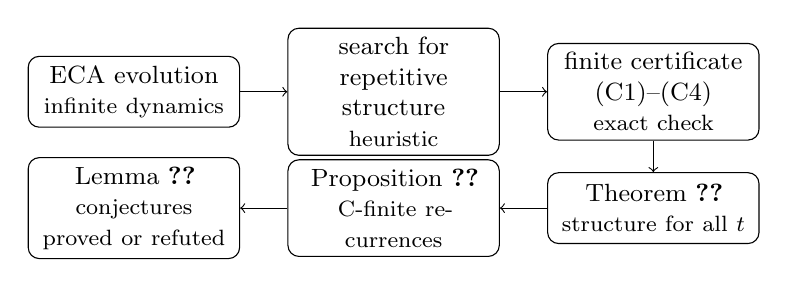
\begin{tikzpicture}[node distance=4mm and 6mm, box/.style={draw,rounded corners,align=center,font=\small,minimum height=9mm,text width=2.45cm}]
\node[box] (a) {ECA evolution\\ \footnotesize infinite dynamics};
\node[box,right=of a] (b) {search for repetitive structure\\ \footnotesize heuristic};
\node[box,right=of b] (c) {finite certificate (C1)--(C4)\\ \footnotesize exact check};
\node[box,below=of c] (d) {Theorem~\ref{thm:cert}\\ \footnotesize structure for all $t$};
\node[box,left=of d] (e) {Proposition~\ref{prop:ann}\\ \footnotesize C-finite recurrences};
\node[box,left=of e] (f) {Lemma~\ref{lem:fin}\\ \footnotesize conjectures proved or refuted};
\draw[->] (a)--(b); \draw[->] (b)--(c); \draw[->] (c)--(d); \draw[->] (d)--(e); \draw[->] (e)--(f);
\end{tikzpicture}
\end{center}
Computation is used only to \emph{find} certificates and to perform finitely many exact checks whose sufficiency is proved. The search itself plays no role in the proofs.

\paragraph{Results.} The outcome is summarised in Table~\ref{tab:summary} and Figure~\ref{fig:bars}.

\begin{table}[ht]\centering
\begin{tabular}{lr}\toprule
OEIS entries in the family with at least one conjecture & 260\\
distinct rules involved & 91\\
rules for which a valid certificate was found & 86\\
conjecture statements extracted & 640\\
\quad proved (Section~\ref{sec:results}, Appendix~\ref{app:proved}) & 575\\
\quad false as stated (Section~\ref{sec:false}) & 15\\
\quad rules without certificate (Rules 129, 137, 167, 169, 182) & 15\\
\quad statements in a format not covered (Appendix~\ref{app:other}) & 35\\
entries with at least one statement proved & 246\\
entries all of whose conjectures are now proved & 205\\\bottomrule
\end{tabular}
\caption{Summary.}\label{tab:summary}
\end{table}

\begin{figure}[ht]\centering
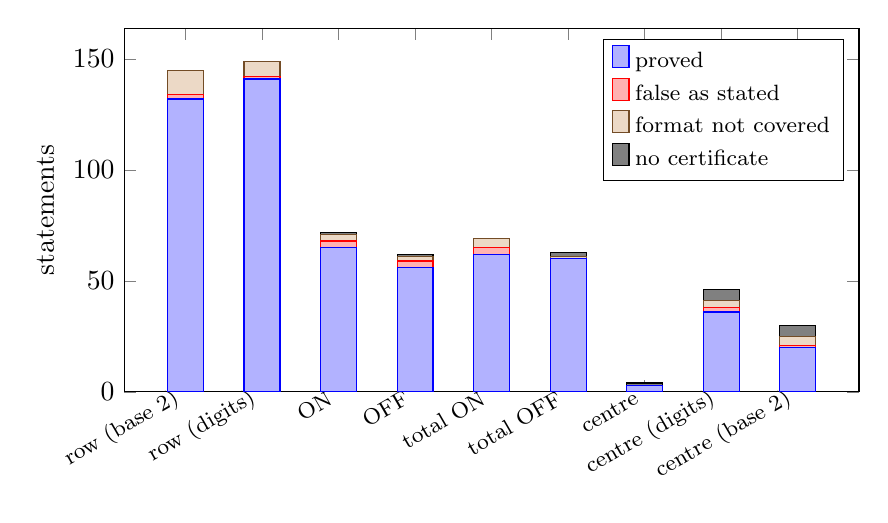
\begin{tikzpicture}
\begin{axis}[ybar stacked, bar width=13pt, width=0.9\textwidth, height=6.2cm,
  symbolic x coords={dec,bin,on,off,ton,toff,mid,mbin,mdec}, xtick=data,
  xticklabels={row (base 2),row (digits),ON,OFF,total ON,total OFF,centre,centre (digits),centre (base 2)},
  x tick label style={rotate=30,anchor=east,font=\footnotesize}, ylabel={statements}, ymin=0,
  legend style={at={(0.98,0.97)},anchor=north east,font=\footnotesize}, legend cell align=left]
\addplot coordinates {(dec,132) (bin,141) (on,65) (off,56) (ton,62) (toff,60) (mid,3) (mbin,36) (mdec,20)};
\addplot coordinates {(dec,2) (bin,1) (on,3) (off,3) (ton,3) (toff,0) (mid,0) (mbin,2) (mdec,1)};
\addplot coordinates {(dec,11) (bin,7) (on,3) (off,2) (ton,4) (toff,1) (mid,0) (mbin,3) (mdec,4)};
\addplot coordinates {(dec,0) (bin,0) (on,1) (off,1) (ton,0) (toff,2) (mid,1) (mbin,5) (mdec,5)};

\legend{proved,false as stated,format not covered,no certificate}
\end{axis}
\end{tikzpicture}
\caption{The 640 statements by type of sequence and outcome.}\label{fig:bars}
\end{figure}

\section{Setting}

Let $f=f_\rho:\{0,1\}^3\to\{0,1\}$ be the local rule, $f(a,b,c)=\lfloor \rho/2^{4a+2b+c}\rfloor \bmod 2$. A configuration is a map $c:\mathbb Z\to\{0,1\}$ and the global map is $F(c)(i)=f(c(i-1),c(i),c(i+1))$. We start from $c_0=\mathbf 1_{\{0\}}$ and put $c_{t+1}=F(c_t)$.

\paragraph{Background.} Let $b_0=0$ and $b_{t+1}=f(b_t,b_t,b_t)$. By induction on $t$, $c_t(i)=b_t$ for $|i|>t$ (the ``light cone''). For rules with $f(0,0,0)=1$ the background is not $0$. The OEIS sequences use the true infinite evolution, and so do we. The sequence $(b_t)$ is periodic from $t=1$ on, with period $1$ or $2$.

\paragraph{Row words.} We encode time $t$ by the word $W_t=c_t(-t-1)\,c_t(-t)\cdots c_t(t+1)\in\{0,1\}^{2t+3}$. Positions in a word are counted from $0$. The first and last letters of $W_t$ equal $b_t$. For a word $W=w_1\cdots w_\ell$ and $b\in\{0,1\}$ put
\[
\Phi_b(W)=b'\,\bigl(f(w_{i-1},w_i,w_{i+1})\bigr)_{i=1}^{\ell}\,b',\qquad b'=f(b,b,b),\quad w_0=w_{\ell+1}=b.
\]
Then $W_{t+1}=\Phi_{b_t}(W_t)$, because the cells $\pm(t+2)$ at time $t+1$ only see background cells.

\paragraph{The nine sequences.} Let $V_t$ be $W_t$ with its first and last letters removed (the cells $-t,\dots,t$). Then the sequences of the family are: $\mathrm{val}_2(V_t)$; $\mathrm{val}_{10}(V_t)$; the number $|V_t|_1$ of ON cells and $2t+1-|V_t|_1$; their partial sums $\sum_{k\le t}$; the centre cell $c_t(0)$, which is the letter of $W_t$ in position $t+1$; and $\sum_{k\le t}c_k(0)\beta^{t-k}$ with $\beta\in\{2,10\}$. Here
\[
\mathrm{val}_\beta(w_1\cdots w_\ell)=\sum_{i=1}^{\ell} w_i\,\beta^{\ell-i},
\]
so that \emph{the exponent attached to a letter is the number of letters to its right}. With these definitions our program reproduces exactly all terms shown in the data fields of the 260 entries.

\section{A pumping lemma and certificates}

For a word $X=x_1\cdots x_\ell$ ($\ell\ge1$) define its \emph{cyclic image} $\widetilde X=(f(x_{i-1},x_i,x_{i+1}))_{i=1}^{\ell}$, with indices modulo $\ell$, and its rotation $\mathrm{rot}_o(X)=x_{o+1}\cdots x_\ell\, x_1\cdots x_o$ ($0\le o<\ell$).

\begin{lemma}[Insertion lemma]\label{lem:ins}
Let $W=P\,B\,B\,Q\,D\,D\,R$ and $W'=P\,B\,B\,B\,Q\,D\,D\,D\,R$, with $B,D$ nonempty. Then, for any $b$, $\Phi_b(W')$ is obtained from $\Phi_b(W)$ by inserting $\widetilde B$ immediately after its first $|P|+|B|+1$ letters, and inserting $\widetilde D$ immediately before its last $|R|+|D|+1$ letters.
\end{lemma}
\begin{proof}
$W'$ arises from $W$ by inserting a copy of $B$ between the two copies of $B$ and a copy of $D$ between the two copies of $D$. Each letter of $\Phi_b(W)$ other than the two boundary letters $b'$ is $f$ applied to a window of three consecutive letters of $bWb$. Every letter of $W$ keeps, in $W'$, the same left and right neighbours. The only letters whose neighbours could change are the last letter of the first $B$ (its right neighbour was the first letter of $B$ and is again the first letter of the inserted $B$), the first letter of the second $B$ (its left neighbour was, and still is, the last letter of a copy of $B$), and the analogous letters around $D$. Hence the images of the old letters are unchanged and keep their order. The letters of the inserted copy of $B$ have as neighbours letters of $BBB$ in the cyclic pattern, so their images form $\widetilde B$; likewise for $D$. Because of the leading letter $b'$, the inserted block follows the first $|P|+|B|+1$ letters of $\Phi_b(W')$; symmetrically on the right.
\end{proof}

\begin{figure}[ht]\centering
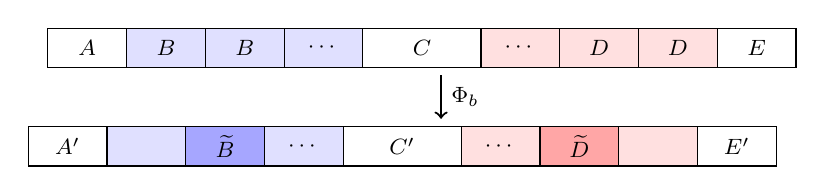
\begin{tikzpicture}[x=5mm,y=5mm,font=\footnotesize]
\tikzset{w/.style={draw,minimum height=5mm,inner sep=1pt,anchor=west}}
\node[w,minimum width=10mm] at (0,2) (A) {$A$};
\node[w,minimum width=10mm,fill=blue!12] at (2,2) {$B$};
\node[w,minimum width=10mm,fill=blue!12] at (4,2) {$B$};
\node[w,minimum width=10mm,fill=blue!12] at (6,2) {$\cdots$};
\node[w,minimum width=15mm] at (8,2) {$C$};
\node[w,minimum width=10mm,fill=red!12] at (11,2) {$\cdots$};
\node[w,minimum width=10mm,fill=red!12] at (13,2) {$D$};
\node[w,minimum width=10mm,fill=red!12] at (15,2) {$D$};
\node[w,minimum width=10mm] at (17,2) {$E$};
\draw[->,thick] (10,1.3)--(10,0.2) node[midway,right]{$\Phi_b$};
\node[w,minimum width=10mm] at (-0.5,-0.5) {$A'$};
\node[w,minimum width=10mm,fill=blue!12] at (1.5,-0.5) {};
\node[w,minimum width=10mm,fill=blue!35] at (3.5,-0.5) {$\widetilde B$};
\node[w,minimum width=10mm,fill=blue!12] at (5.5,-0.5) {$\cdots$};
\node[w,minimum width=15mm] at (7.5,-0.5) {$C'$};
\node[w,minimum width=10mm,fill=red!12] at (10.5,-0.5) {$\cdots$};
\node[w,minimum width=10mm,fill=red!35] at (12.5,-0.5) {$\widetilde D$};
\node[w,minimum width=10mm,fill=red!12] at (14.5,-0.5) {};
\node[w,minimum width=10mm] at (16.5,-0.5) {$E'$};
\end{tikzpicture}
\caption{Lemma~\ref{lem:ins}: one more copy of $B$ (resp.\ $D$) in the row produces one more copy of $\widetilde B$ (resp.\ $\widetilde D$) at a fixed distance from the left (resp.\ right) end of the next row. In a valid certificate $\widetilde B$ and $\widetilde D$ are rotations of the blocks of the next row, so the next row has the same shape, with the exponent $m$ preserved.}\label{fig:ins}
\end{figure}

\begin{definition}[Certificate]\label{def:cert}
A \emph{certificate} for rule $\rho$ consists of integers $p\ge1$, $t_0\ge0$, $\ell_B,\ell_D\ge1$ with $\ell_B+\ell_D=2p$, and words $A_r,B_r,C_r,D_r,E_r$ $(0\le r<p)$ with $|A_r|,|E_r|\ge1$, $|B_r|=\ell_B$, $|D_r|=\ell_D$. Write $\Omega(r,m)=A_rB_r^mC_rD_r^mE_r$. For $r<p-1$ put $(r',\delta)=(r+1,0)$, and for $r=p-1$ put $(r',\delta)=(0,1)$. The certificate is \emph{valid} if
\begin{enumerate}
\item[(C1)] $W_{t_0+2p}=\Omega(0,2)$;
\item[(C2)] $b_{t_0+r+pm}=b_{t_0+r+2p}$ for $2\le m\le 5$ and all $r$;
\item[(C3)] for every $r$, with $b=b_{t_0+r+2p}$: $\Phi_b(\Omega(r,2))=\Omega(r',2+\delta)$;
\item[(C4)] for every $r$, putting $o=|A_r|+\ell_B+1-|A_{r'}|$ and $o'=|E_r|+\ell_D+1-|E_{r'}|$: $0\le o\le(2+\delta)\ell_B$, $0\le o'\le(2+\delta)\ell_D$, $\widetilde{B_r}=\mathrm{rot}_{o\bmod \ell_B}(B_{r'})$, $\widetilde{D_r}=\mathrm{rot}_{(-o')\bmod \ell_D}(D_{r'})$, and $|A_r|+\ell_B+1\le |\Omega(r',2+\delta)|-(|E_r|+\ell_D+1)$.
\end{enumerate}
\end{definition}

\begin{theorem}\label{thm:cert}
If rule $\rho$ has a valid certificate, then $W_{t_0+r+pm}=\Omega(r,m)$ for all $0\le r<p$ and all $m\ge2$. In particular, for $t\ge T:=t_0+2p$ every row has the shape $A\,B^m\,C\,D^m\,E$ described by the certificate.
\end{theorem}
\begin{proof}
Since $(b_t)_{t\ge1}$ has period dividing $2$, (C2) implies that $b_{t_0+r+pm}$ does not depend on $m\ge2$. We show by induction along $t=t_0+r+pm$ ($m\ge2$) that $W_t=\Omega(r,m)$. The base $t=t_0+2p$ is (C1). Assume $W_t=\Omega(r,m)$ with $m\ge2$. For $k\ge2$, $\Omega(r,k+1)$ arises from $\Omega(r,k)$ by inserting a copy of $B_r$ between the first two copies and a copy of $D_r$ between the last two, so Lemma~\ref{lem:ins} applies with $P=A_r$, $R=E_r$. Applying it $m-2$ times, $\Phi_b(\Omega(r,m))$ equals $\Phi_b(\Omega(r,2))$ with $m-2$ copies of $\widetilde{B_r}$ inserted after the first $|A_r|+\ell_B+1$ letters and $m-2$ copies of $\widetilde{D_r}$ inserted before the last $|E_r|+\ell_D+1$ letters. The two insertion points do not cross, by the last condition of (C4). By (C3), $\Phi_b(\Omega(r,2))=\Omega(r',2+\delta)$. In $\Omega(r',k)$ the left insertion point lies at offset $o$ inside (or at an end of) the run $B_{r'}^k$. Inserting there the word $\mathrm{rot}_{o\bmod\ell_B}(B_{r'})$ turns $B_{r'}^k$ into $B_{r'}^{k+1}$ and leaves the prefix unchanged, so repeated insertions at the same place are possible. The same holds on the right for $D_{r'}$, with the suffix unchanged. By (C4) and induction on the number of insertions, $\Phi_b(\Omega(r,m))=\Omega(r',m+\delta)$. Since $W_{t+1}=\Phi_{b_t}(W_t)$ and $t+1=t_0+r'+p(m+\delta)$, this is the claim for $t+1$.
\end{proof}

\begin{figure}[ht]\centering
\scalebox{0.9}{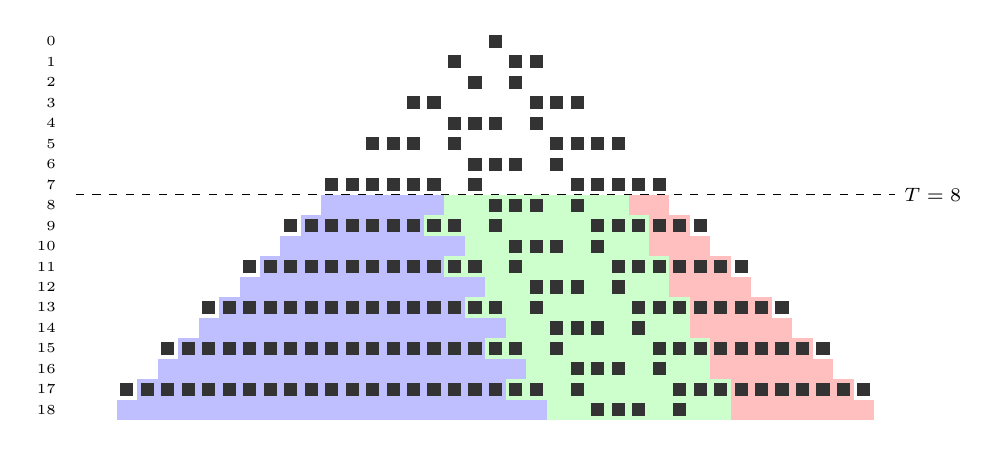
\begin{tikzpicture}[x=2.6mm,y=-2.6mm]
\fill[black!80] (0.18,0.18) rectangle (0.82,0.82);
\node[anchor=east,font=\tiny] at (-20.5,0.5) {0};
\fill[black!80] (-1.82,1.18) rectangle (-1.1800000000000002,1.8199999999999998);
\fill[black!80] (1.18,1.18) rectangle (1.8199999999999998,1.8199999999999998);
\fill[black!80] (2.18,1.18) rectangle (2.82,1.8199999999999998);
\node[anchor=east,font=\tiny] at (-20.5,1.5) {1};
\fill[black!80] (-0.8200000000000001,2.18) rectangle (-0.18000000000000005,2.82);
\fill[black!80] (1.18,2.18) rectangle (1.8199999999999998,2.82);
\node[anchor=east,font=\tiny] at (-20.5,2.5) {2};
\fill[black!80] (-3.82,3.18) rectangle (-3.18,3.82);
\fill[black!80] (-2.82,3.18) rectangle (-2.18,3.82);
\fill[black!80] (2.18,3.18) rectangle (2.82,3.82);
\fill[black!80] (3.18,3.18) rectangle (3.82,3.82);
\fill[black!80] (4.18,3.18) rectangle (4.82,3.82);
\node[anchor=east,font=\tiny] at (-20.5,3.5) {3};
\fill[black!80] (-1.82,4.18) rectangle (-1.1800000000000002,4.82);
\fill[black!80] (-0.8200000000000001,4.18) rectangle (-0.18000000000000005,4.82);
\fill[black!80] (0.18,4.18) rectangle (0.82,4.82);
\fill[black!80] (2.18,4.18) rectangle (2.82,4.82);
\node[anchor=east,font=\tiny] at (-20.5,4.5) {4};
\fill[black!80] (-5.82,5.18) rectangle (-5.18,5.82);
\fill[black!80] (-4.82,5.18) rectangle (-4.18,5.82);
\fill[black!80] (-3.82,5.18) rectangle (-3.18,5.82);
\fill[black!80] (-1.82,5.18) rectangle (-1.1800000000000002,5.82);
\fill[black!80] (3.18,5.18) rectangle (3.82,5.82);
\fill[black!80] (4.18,5.18) rectangle (4.82,5.82);
\fill[black!80] (5.18,5.18) rectangle (5.82,5.82);
\fill[black!80] (6.18,5.18) rectangle (6.82,5.82);
\node[anchor=east,font=\tiny] at (-20.5,5.5) {5};
\fill[black!80] (-0.8200000000000001,6.18) rectangle (-0.18000000000000005,6.82);
\fill[black!80] (0.18,6.18) rectangle (0.82,6.82);
\fill[black!80] (1.18,6.18) rectangle (1.8199999999999998,6.82);
\fill[black!80] (3.18,6.18) rectangle (3.82,6.82);
\node[anchor=east,font=\tiny] at (-20.5,6.5) {6};
\fill[black!80] (-7.82,7.18) rectangle (-7.18,7.82);
\fill[black!80] (-6.82,7.18) rectangle (-6.18,7.82);
\fill[black!80] (-5.82,7.18) rectangle (-5.18,7.82);
\fill[black!80] (-4.82,7.18) rectangle (-4.18,7.82);
\fill[black!80] (-3.82,7.18) rectangle (-3.18,7.82);
\fill[black!80] (-2.82,7.18) rectangle (-2.18,7.82);
\fill[black!80] (-0.8200000000000001,7.18) rectangle (-0.18000000000000005,7.82);
\fill[black!80] (4.18,7.18) rectangle (4.82,7.82);
\fill[black!80] (5.18,7.18) rectangle (5.82,7.82);
\fill[black!80] (6.18,7.18) rectangle (6.82,7.82);
\fill[black!80] (7.18,7.18) rectangle (7.82,7.82);
\fill[black!80] (8.18,7.18) rectangle (8.82,7.82);
\node[anchor=east,font=\tiny] at (-20.5,7.5) {7};
\fill[blue!25] (-8,8) rectangle (-2,9);
\fill[red!25] (7,8) rectangle (9,9);
\fill[green!20] (-2,8) rectangle (7,9);
\fill[black!80] (0.18,8.18) rectangle (0.82,8.82);
\fill[black!80] (1.18,8.18) rectangle (1.8199999999999998,8.82);
\fill[black!80] (2.18,8.18) rectangle (2.82,8.82);
\fill[black!80] (4.18,8.18) rectangle (4.82,8.82);
\node[anchor=east,font=\tiny] at (-20.5,8.5) {8};
\fill[blue!25] (-9,9) rectangle (-3,10);
\fill[red!25] (8,9) rectangle (10,10);
\fill[green!20] (-3,9) rectangle (8,10);
\fill[black!80] (-9.82,9.18) rectangle (-9.18,9.82);
\fill[black!80] (-8.82,9.18) rectangle (-8.18,9.82);
\fill[black!80] (-7.82,9.18) rectangle (-7.18,9.82);
\fill[black!80] (-6.82,9.18) rectangle (-6.18,9.82);
\fill[black!80] (-5.82,9.18) rectangle (-5.18,9.82);
\fill[black!80] (-4.82,9.18) rectangle (-4.18,9.82);
\fill[black!80] (-3.82,9.18) rectangle (-3.18,9.82);
\fill[black!80] (-2.82,9.18) rectangle (-2.18,9.82);
\fill[black!80] (-1.82,9.18) rectangle (-1.1800000000000002,9.82);
\fill[black!80] (0.18,9.18) rectangle (0.82,9.82);
\fill[black!80] (5.18,9.18) rectangle (5.82,9.82);
\fill[black!80] (6.18,9.18) rectangle (6.82,9.82);
\fill[black!80] (7.18,9.18) rectangle (7.82,9.82);
\fill[black!80] (8.18,9.18) rectangle (8.82,9.82);
\fill[black!80] (9.18,9.18) rectangle (9.82,9.82);
\fill[black!80] (10.18,9.18) rectangle (10.82,9.82);
\node[anchor=east,font=\tiny] at (-20.5,9.5) {9};
\fill[blue!25] (-10,10) rectangle (-1,11);
\fill[red!25] (8,10) rectangle (11,11);
\fill[green!20] (-1,10) rectangle (8,11);
\fill[black!80] (1.18,10.18) rectangle (1.8199999999999998,10.82);
\fill[black!80] (2.18,10.18) rectangle (2.82,10.82);
\fill[black!80] (3.18,10.18) rectangle (3.82,10.82);
\fill[black!80] (5.18,10.18) rectangle (5.82,10.82);
\node[anchor=east,font=\tiny] at (-20.5,10.5) {10};
\fill[blue!25] (-11,11) rectangle (-2,12);
\fill[red!25] (9,11) rectangle (12,12);
\fill[green!20] (-2,11) rectangle (9,12);
\fill[black!80] (-11.82,11.18) rectangle (-11.18,11.82);
\fill[black!80] (-10.82,11.18) rectangle (-10.18,11.82);
\fill[black!80] (-9.82,11.18) rectangle (-9.18,11.82);
\fill[black!80] (-8.82,11.18) rectangle (-8.18,11.82);
\fill[black!80] (-7.82,11.18) rectangle (-7.18,11.82);
\fill[black!80] (-6.82,11.18) rectangle (-6.18,11.82);
\fill[black!80] (-5.82,11.18) rectangle (-5.18,11.82);
\fill[black!80] (-4.82,11.18) rectangle (-4.18,11.82);
\fill[black!80] (-3.82,11.18) rectangle (-3.18,11.82);
\fill[black!80] (-2.82,11.18) rectangle (-2.18,11.82);
\fill[black!80] (-1.82,11.18) rectangle (-1.1800000000000002,11.82);
\fill[black!80] (-0.8200000000000001,11.18) rectangle (-0.18000000000000005,11.82);
\fill[black!80] (1.18,11.18) rectangle (1.8199999999999998,11.82);
\fill[black!80] (6.18,11.18) rectangle (6.82,11.82);
\fill[black!80] (7.18,11.18) rectangle (7.82,11.82);
\fill[black!80] (8.18,11.18) rectangle (8.82,11.82);
\fill[black!80] (9.18,11.18) rectangle (9.82,11.82);
\fill[black!80] (10.18,11.18) rectangle (10.82,11.82);
\fill[black!80] (11.18,11.18) rectangle (11.82,11.82);
\fill[black!80] (12.18,11.18) rectangle (12.82,11.82);
\node[anchor=east,font=\tiny] at (-20.5,11.5) {11};
\fill[blue!25] (-12,12) rectangle (0,13);
\fill[red!25] (9,12) rectangle (13,13);
\fill[green!20] (0,12) rectangle (9,13);
\fill[black!80] (2.18,12.18) rectangle (2.82,12.82);
\fill[black!80] (3.18,12.18) rectangle (3.82,12.82);
\fill[black!80] (4.18,12.18) rectangle (4.82,12.82);
\fill[black!80] (6.18,12.18) rectangle (6.82,12.82);
\node[anchor=east,font=\tiny] at (-20.5,12.5) {12};
\fill[blue!25] (-13,13) rectangle (-1,14);
\fill[red!25] (10,13) rectangle (14,14);
\fill[green!20] (-1,13) rectangle (10,14);
\fill[black!80] (-13.82,13.18) rectangle (-13.18,13.82);
\fill[black!80] (-12.82,13.18) rectangle (-12.18,13.82);
\fill[black!80] (-11.82,13.18) rectangle (-11.18,13.82);
\fill[black!80] (-10.82,13.18) rectangle (-10.18,13.82);
\fill[black!80] (-9.82,13.18) rectangle (-9.18,13.82);
\fill[black!80] (-8.82,13.18) rectangle (-8.18,13.82);
\fill[black!80] (-7.82,13.18) rectangle (-7.18,13.82);
\fill[black!80] (-6.82,13.18) rectangle (-6.18,13.82);
\fill[black!80] (-5.82,13.18) rectangle (-5.18,13.82);
\fill[black!80] (-4.82,13.18) rectangle (-4.18,13.82);
\fill[black!80] (-3.82,13.18) rectangle (-3.18,13.82);
\fill[black!80] (-2.82,13.18) rectangle (-2.18,13.82);
\fill[black!80] (-1.82,13.18) rectangle (-1.1800000000000002,13.82);
\fill[black!80] (-0.8200000000000001,13.18) rectangle (-0.18000000000000005,13.82);
\fill[black!80] (0.18,13.18) rectangle (0.82,13.82);
\fill[black!80] (2.18,13.18) rectangle (2.82,13.82);
\fill[black!80] (7.18,13.18) rectangle (7.82,13.82);
\fill[black!80] (8.18,13.18) rectangle (8.82,13.82);
\fill[black!80] (9.18,13.18) rectangle (9.82,13.82);
\fill[black!80] (10.18,13.18) rectangle (10.82,13.82);
\fill[black!80] (11.18,13.18) rectangle (11.82,13.82);
\fill[black!80] (12.18,13.18) rectangle (12.82,13.82);
\fill[black!80] (13.18,13.18) rectangle (13.82,13.82);
\fill[black!80] (14.18,13.18) rectangle (14.82,13.82);
\node[anchor=east,font=\tiny] at (-20.5,13.5) {13};
\fill[blue!25] (-14,14) rectangle (1,15);
\fill[red!25] (10,14) rectangle (15,15);
\fill[green!20] (1,14) rectangle (10,15);
\fill[black!80] (3.18,14.18) rectangle (3.82,14.82);
\fill[black!80] (4.18,14.18) rectangle (4.82,14.82);
\fill[black!80] (5.18,14.18) rectangle (5.82,14.82);
\fill[black!80] (7.18,14.18) rectangle (7.82,14.82);
\node[anchor=east,font=\tiny] at (-20.5,14.5) {14};
\fill[blue!25] (-15,15) rectangle (0,16);
\fill[red!25] (11,15) rectangle (16,16);
\fill[green!20] (0,15) rectangle (11,16);
\fill[black!80] (-15.82,15.18) rectangle (-15.18,15.82);
\fill[black!80] (-14.82,15.18) rectangle (-14.18,15.82);
\fill[black!80] (-13.82,15.18) rectangle (-13.18,15.82);
\fill[black!80] (-12.82,15.18) rectangle (-12.18,15.82);
\fill[black!80] (-11.82,15.18) rectangle (-11.18,15.82);
\fill[black!80] (-10.82,15.18) rectangle (-10.18,15.82);
\fill[black!80] (-9.82,15.18) rectangle (-9.18,15.82);
\fill[black!80] (-8.82,15.18) rectangle (-8.18,15.82);
\fill[black!80] (-7.82,15.18) rectangle (-7.18,15.82);
\fill[black!80] (-6.82,15.18) rectangle (-6.18,15.82);
\fill[black!80] (-5.82,15.18) rectangle (-5.18,15.82);
\fill[black!80] (-4.82,15.18) rectangle (-4.18,15.82);
\fill[black!80] (-3.82,15.18) rectangle (-3.18,15.82);
\fill[black!80] (-2.82,15.18) rectangle (-2.18,15.82);
\fill[black!80] (-1.82,15.18) rectangle (-1.1800000000000002,15.82);
\fill[black!80] (-0.8200000000000001,15.18) rectangle (-0.18000000000000005,15.82);
\fill[black!80] (0.18,15.18) rectangle (0.82,15.82);
\fill[black!80] (1.18,15.18) rectangle (1.8199999999999998,15.82);
\fill[black!80] (3.18,15.18) rectangle (3.82,15.82);
\fill[black!80] (8.18,15.18) rectangle (8.82,15.82);
\fill[black!80] (9.18,15.18) rectangle (9.82,15.82);
\fill[black!80] (10.18,15.18) rectangle (10.82,15.82);
\fill[black!80] (11.18,15.18) rectangle (11.82,15.82);
\fill[black!80] (12.18,15.18) rectangle (12.82,15.82);
\fill[black!80] (13.18,15.18) rectangle (13.82,15.82);
\fill[black!80] (14.18,15.18) rectangle (14.82,15.82);
\fill[black!80] (15.18,15.18) rectangle (15.82,15.82);
\fill[black!80] (16.18,15.18) rectangle (16.82,15.82);
\node[anchor=east,font=\tiny] at (-20.5,15.5) {15};
\fill[blue!25] (-16,16) rectangle (2,17);
\fill[red!25] (11,16) rectangle (17,17);
\fill[green!20] (2,16) rectangle (11,17);
\fill[black!80] (4.18,16.18) rectangle (4.82,16.82);
\fill[black!80] (5.18,16.18) rectangle (5.82,16.82);
\fill[black!80] (6.18,16.18) rectangle (6.82,16.82);
\fill[black!80] (8.18,16.18) rectangle (8.82,16.82);
\node[anchor=east,font=\tiny] at (-20.5,16.5) {16};
\fill[blue!25] (-17,17) rectangle (1,18);
\fill[red!25] (12,17) rectangle (18,18);
\fill[green!20] (1,17) rectangle (12,18);
\fill[black!80] (-17.82,17.18) rectangle (-17.18,17.82);
\fill[black!80] (-16.82,17.18) rectangle (-16.18,17.82);
\fill[black!80] (-15.82,17.18) rectangle (-15.18,17.82);
\fill[black!80] (-14.82,17.18) rectangle (-14.18,17.82);
\fill[black!80] (-13.82,17.18) rectangle (-13.18,17.82);
\fill[black!80] (-12.82,17.18) rectangle (-12.18,17.82);
\fill[black!80] (-11.82,17.18) rectangle (-11.18,17.82);
\fill[black!80] (-10.82,17.18) rectangle (-10.18,17.82);
\fill[black!80] (-9.82,17.18) rectangle (-9.18,17.82);
\fill[black!80] (-8.82,17.18) rectangle (-8.18,17.82);
\fill[black!80] (-7.82,17.18) rectangle (-7.18,17.82);
\fill[black!80] (-6.82,17.18) rectangle (-6.18,17.82);
\fill[black!80] (-5.82,17.18) rectangle (-5.18,17.82);
\fill[black!80] (-4.82,17.18) rectangle (-4.18,17.82);
\fill[black!80] (-3.82,17.18) rectangle (-3.18,17.82);
\fill[black!80] (-2.82,17.18) rectangle (-2.18,17.82);
\fill[black!80] (-1.82,17.18) rectangle (-1.1800000000000002,17.82);
\fill[black!80] (-0.8200000000000001,17.18) rectangle (-0.18000000000000005,17.82);
\fill[black!80] (0.18,17.18) rectangle (0.82,17.82);
\fill[black!80] (1.18,17.18) rectangle (1.8199999999999998,17.82);
\fill[black!80] (2.18,17.18) rectangle (2.82,17.82);
\fill[black!80] (4.18,17.18) rectangle (4.82,17.82);
\fill[black!80] (9.18,17.18) rectangle (9.82,17.82);
\fill[black!80] (10.18,17.18) rectangle (10.82,17.82);
\fill[black!80] (11.18,17.18) rectangle (11.82,17.82);
\fill[black!80] (12.18,17.18) rectangle (12.82,17.82);
\fill[black!80] (13.18,17.18) rectangle (13.82,17.82);
\fill[black!80] (14.18,17.18) rectangle (14.82,17.82);
\fill[black!80] (15.18,17.18) rectangle (15.82,17.82);
\fill[black!80] (16.18,17.18) rectangle (16.82,17.82);
\fill[black!80] (17.18,17.18) rectangle (17.82,17.82);
\fill[black!80] (18.18,17.18) rectangle (18.82,17.82);
\node[anchor=east,font=\tiny] at (-20.5,17.5) {17};
\fill[blue!25] (-18,18) rectangle (3,19);
\fill[red!25] (12,18) rectangle (19,19);
\fill[green!20] (3,18) rectangle (12,19);
\fill[black!80] (5.18,18.18) rectangle (5.82,18.82);
\fill[black!80] (6.18,18.18) rectangle (6.82,18.82);
\fill[black!80] (7.18,18.18) rectangle (7.82,18.82);
\fill[black!80] (9.18,18.18) rectangle (9.82,18.82);
\node[anchor=east,font=\tiny] at (-20.5,18.5) {18};
\draw[dashed] (-20,8) -- (20,8) node[right,font=\scriptsize]{$T=8$};
\end{tikzpicture}}
\caption{Rule 25, $t\le 18$. A valid certificate has $p=2$, $t_0=4$, $\ell_B=3$, $\ell_D=1$, so the structure is guaranteed from $T=8$ on (dashed line). For $t\ge T$ the run $B_r^m$ is shaded blue, $C_r$ green and the run $D_r^m$ red; black squares are ON cells. For instance $W_{5+2m}=1\,(111)^m\,11010000111\,(1)^m\,1$ for $m\ge2$. The pattern drifts to the right, because the left run grows three cells every two steps and the right run only one.}\label{fig:spacetime}
\end{figure}

\begin{remark}[Boundary cases in (C1)--(C4)]\label{rem:edge}
(i) Blocks of length one are allowed: if $\ell_B=1$ the inserted letter has two neighbours equal to itself, and $\widetilde B=f(x,x,x)$. (ii) The offsets $o=0$ and $o=(2+\delta)\ell_B$ are allowed: they mean that the insertion happens exactly at the beginning or at the end of the run $B_{r'}^{2+\delta}$. In both cases inserting $\mathrm{rot}_{o\bmod\ell_B}(B_{r'})=B_{r'}$ again yields a run of the same block, so the argument of Theorem~\ref{thm:cert} applies verbatim. (iii) $C_r$ may be empty; then the two runs are adjacent, and the last condition of (C4) still guarantees that the left insertion point does not lie to the right of the right one, so that the two insertions commute. (iv) The requirement $|A_r|,|E_r|\ge1$ ensures that the first and last letters of $W_t$, which are background letters, are never inside a run; it is used in Proposition~\ref{prop:ann} to pass from $W_t$ to $V_t$. (v) In (C2) four values of $m$ suffice, because $(b_t)_{t\ge1}$ has period $1$ or $2$ and $t_0+r+2p\ge1$. (vi) Conditions (C3) and (C4) involve only $\Omega(r,2)$ and $\Omega(r',2+\delta)$, words of length at most $|W_{t_0+3p}|$, so validity is a finite check, which takes milliseconds.
\end{remark}

\section{The certificate search}\label{sec:search}

\paragraph{Algorithm.} For a given rule we simulate $W_t$ for $t\le t_0^{\max}+8p^{\max}+5$ and enumerate, in this order, $p=1,2,\dots,p^{\max}$, then $t_0=0,1,\dots,t_0^{\max}-1$, then $\ell_B=p$ followed by the other values $1\le\ell_B<2p$. For each choice and each residue $r$ we look for the shortest $A_r$ and then the shortest $E_r$ such that the rows $W_{t_0+r+pm}$, $2\le m\le 6$, all have the form $A_rB_r^mC_rD_r^mE_r$ with $|B_r|=\ell_B$, $|D_r|=2p-\ell_B$; the words are read off $W_{t_0+r+2p}$. The first candidate that passes (C1)--(C4) is returned. For a row of length $n$ the inner search costs $O(n^2)$ comparisons of words of length $O(n)$, so the total cost is polynomial and modest: the default search over all 91 rules takes 69 seconds on a single core of a standard machine, at most 12 seconds for a single rule, about two thirds of it spent on the five rules for which none is found.

\paragraph{Choice of the limits.} We used $p^{\max}=12$ and $t_0^{\max}=40$. The bound on $t_0$ is generous, and the bound on $p$ is the smallest one that certifies every rule we could certify: the smallest period of a valid certificate is $p=1$ for 25 rules, $p=2$ for 49 rules, $p=4$ for 10 rules, $p=12$ for 2 rules, and the smallest $t_0$ for that period is at most 5. Rules 109 and 131 need $p=12$, so a smaller bound would leave them out. Enlarging the limits does not change the outcome for the five rules without certificate: with $p^{\max}=24$ and $t_0^{\max}=80$ the search, run for 38 minutes in total, finds no certificate for any of them. This is expected: Rules 129, 137, 167, 169 and 182 have nested (Sierpi\'nski-like) or irregular space-time diagrams, in which the length of the non-periodic part appears to grow without bound. We therefore expect that no certificate of the shape $AB^mCD^mE$ exists for them, for any $p$ and $t_0$, but we have not proved this.

\paragraph{Alternative certificates and robustness.} Certificates are not unique. In practice, when $(p,t_0,\dots)$ is valid, one also finds valid certificates with period $kp$ or with a larger $t_0$. Within the limits $p\le12$, $t_0<40$, every certified rule has many valid certificates (between 39 and 5760, counting each choice of $(p,t_0,\ell_B)$ once); for instance, the valid periods of Rule~37 are $p\in\{2,4,6,8,10,12\}$. Different valid certificates for the same rule describe the same rows (Theorem~\ref{thm:cert} determines $W_t$), hence give the same sequences; they may give different annihilating polynomials, but every conclusion drawn from Lemma~\ref{lem:fin} is a statement about the sequence and does not depend on the certificate used. The search depends on implementation choices (the order of enumeration, the preference for short $A_r$ and $E_r$, the range $2\le m\le6$ used to read candidates), but only through \emph{which} certificate is found, never through the validity of the conclusions, which rests on the exact check of (C1)--(C4) alone.


\section{Linear recurrences for the nine sequences}

Let $S$ denote the forward shift, $(Su)(t)=u(t+1)$. For a polynomial $P(S)=\sum_i \pi_iS^i$ we say that $P$ \emph{annihilates $u$ from $N$ on} if $\sum_i\pi_iu(t+i)=0$ for all $t\ge N$. Throughout this section we fix a valid certificate and put
\[
T=t_0+2p,\qquad L=\max_r|A_rB_rC_rD_rE_r|,\qquad
\pi=\begin{cases}p,&\ell_B=p,\\ p\,\ell_B\ell_D,&\ell_B\ne p,\end{cases}\qquad
N_{\mathrm c}=t_0+p\,(L+t_0+p+4).
\]
For $t\ge T$ we write $t=t_0+r+pm$ with $0\le r<p$ and $m\ge2$. Note that $t\mapsto t+p$ corresponds to $m\mapsto m+1$ with $r$ fixed, so that, for a constant $\lambda$, $(S^p-\lambda)$ annihilates from $T$ on any sequence equal to $\gamma_r\lambda^m$ on each residue class.

\begin{proposition}\label{prop:ann}
Let $\beta\in\{2,10\}$.
\begin{enumerate}
\item $\mathrm{val}_\beta(V_t)$ is annihilated from $T$ on by $(S^p-1)(S^p-\beta^{\ell_D})(S^p-\beta^{2p})$.
\item The numbers of ON cells and of OFF cells in $V_t$ are annihilated from $T$ on by $(S^p-1)^2$, and their running totals by $(S-1)(S^p-1)^2$.
\item The centre cell $c_t(0)$ is annihilated from $N_{\mathrm c}$ on by $S^\pi-1$, and $\sum_{k\le t}c_k(0)\beta^{t-k}$ by $(S^\pi-1)(S-\beta)$.
\end{enumerate}
\end{proposition}

\begin{proof}
Fix $r$ and $m\ge 2$. By Theorem~\ref{thm:cert}, $V_t=A'\,B^m\,C\,D^m\,E'$, where $B=B_r$, $C=C_r$, $D=D_r$, and $A'$ (resp.\ $E'$) is $A_r$ without its first letter (resp.\ $E_r$ without its last letter). Put $c=|C|$ and $e=|E'|$.

\emph{(1)} For words $X_1,\dots,X_k$ we have $\mathrm{val}_\beta(X_1\cdots X_k)=\sum_{i}\mathrm{val}_\beta(X_i)\,\beta^{|X_{i+1}\cdots X_k|}$, and $\mathrm{val}_\beta(X^m)=\mathrm{val}_\beta(X)\,\frac{\beta^{m|X|}-1}{\beta^{|X|}-1}$. Applying this to the five factors of $V_t$, and recording for each factor the number of letters to its right,
\begin{align*}
\mathrm{val}_\beta(V_t)
&=\mathrm{val}_\beta(A')\,\beta^{m\ell_B+c+m\ell_D+e}
+\mathrm{val}_\beta(B)\,\frac{\beta^{m\ell_B}-1}{\beta^{\ell_B}-1}\,\beta^{c+m\ell_D+e}
+\mathrm{val}_\beta(C)\,\beta^{m\ell_D+e}\\
&\quad+\mathrm{val}_\beta(D)\,\frac{\beta^{m\ell_D}-1}{\beta^{\ell_D}-1}\,\beta^{e}
+\mathrm{val}_\beta(E').
\end{align*}
The second summand equals $\frac{\mathrm{val}_\beta(B)\beta^{c+e}}{\beta^{\ell_B}-1}\bigl(\beta^{m(\ell_B+\ell_D)}-\beta^{m\ell_D}\bigr)$. Using $\ell_B+\ell_D=2p$ we obtain
\[
\mathrm{val}_\beta(V_t)=\gamma_{r,0}+\gamma_{r,1}\,\bigl(\beta^{\ell_D}\bigr)^m+\gamma_{r,2}\,\bigl(\beta^{2p}\bigr)^m
\]
with rational constants $\gamma_{r,i}$ depending only on $r$. Each factor $S^p-\lambda$, $\lambda\in\{1,\beta^{\ell_D},\beta^{2p}\}$, kills the corresponding term, and the three factors commute, which proves (1).

\begin{remark}\label{rem:lD}
The middle root is $\beta^{\ell_D}$, not $\beta^{\ell_B}$. The digits of the $B$-run lie to the left of the whole $D$-run, so every letter of $B^m$ carries the factor $\beta^{m\ell_D}$; the growth of the $B$-run itself only appears combined with it, as $\beta^{m(\ell_B+\ell_D)}$. A term $\beta^{m\ell_B}$ would appear if the rows were read from right to left. When $\ell_B=\ell_D=p$ (73 of the 86 certified rules) the two expressions coincide. For the 13 rules with $\ell_B\neq\ell_D$, the polynomial with $\beta^{\ell_B}$ in place of $\beta^{\ell_D}$ indeed fails to annihilate the sequence in 22 of the 26 cases (rule, base); this is checked by the accompanying code. Independently of the proof above, the code also confirms the three statements of the proposition numerically for all certified rules and all nine sequences on $300$ consecutive values of $t$ beyond the threshold ($232{,}200$ identities, no exception).
\end{remark}

\emph{(2)} $|V_t|_1=|A'CE'|_1+m\,(|B|_1+|D|_1)$ is affine in $m$, and so is $2t+1-|V_t|_1=2(t_0+r+pm)+1-|V_t|_1$. Since $(S^p-1)^2$ kills every sequence of the form $\gamma+\gamma'm$ on each residue class, both counts are annihilated from $T$ on. If $\tau(t)=\sum_{k\le t}\nu(k)$ is a running total, then $(S-1)\tau(t)=\nu(t+1)$, hence $(S^p-1)^2(S-1)\tau(t)=\bigl((S^p-1)^2\nu\bigr)(t+1)=0$ for $t+1\ge T$, in particular for $t\ge T$.

\emph{(3)} The centre cell is the letter of $W_t=\Omega(r,m)$ in position $j=t+1=t_0+r+1+pm$. In $\Omega(r,m)$ the $B$-run occupies the positions $[\,|A_r|,\,|A_r|+m\ell_B)$, then $C_r$ follows, then the $D$-run occupies $[\,|A_r|+m\ell_B+c,\ |A_r|+m\ell_B+c+m\ell_D)$. Put $\kappa=t_0+r+1-|A_r|$, so that $1-L\le\kappa\le t_0+p$, and let $\varepsilon(m)=j-(|A_r|+m\ell_B)=\kappa+m(p-\ell_B)$ be the offset of the centre from the beginning of $C_r$. Let $m_1=L+t_0+p+1$. We show that for $m\ge m_1$ the centre lies in a region determined by $r$ alone, at an offset that is constant, or periodic in $m$, modulo the length of the repeated block.

\emph{Case $\ell_B=p$.} Then $\varepsilon=\kappa$ does not depend on $m$. If $0\le\kappa<c$, the centre is the letter of $C_r$ in position $\kappa$. If $\kappa<0$, then $j-|A_r|=\kappa+mp\ge 1-L+m\ge0$ and $j<|A_r|+m\ell_B$, so the centre is the letter of $B_r$ in position $(\kappa+mp)\bmod p=\kappa\bmod p$. If $\kappa\ge c$, then $0\le\kappa-c\le t_0+p-1<mp=m\ell_D$, so the centre is the letter of $D_r$ in position $(\kappa-c)\bmod p$. In all three cases $c_t(0)$ depends only on $r$.

\emph{Case $\ell_B<p$.} Then $\varepsilon(m)\ge\kappa+m=t_0+r+1-|A_r|+m\ge c$, because $m\ge L\ge|A_r|+|C_r|$, and $\varepsilon(m)-c<m\ell_D$ because $\varepsilon(m)-c-m\ell_D=\kappa-c-mp\le t_0+p-1-mp<0$. So the centre lies in the $D$-run, and it is the letter of $D_r$ in position $(\kappa-c+m(p-\ell_B))\bmod\ell_D$, which is periodic in $m$ with period dividing $\ell_D$.

\emph{Case $\ell_B>p$.} Then $j-|A_r|=\kappa+mp\ge 1-L+m\ge0$ and $j-|A_r|-m\ell_B=\kappa-m(\ell_B-p)\le t_0+p-m<0$. So the centre lies in the $B$-run and is the letter of $B_r$ in position $(\kappa+mp)\bmod\ell_B$, which is periodic in $m$ with period dividing $\ell_B$.

Consequently, if $m\ge m_1$ then $c_{t+\pi}(0)=c_t(0)$, where $t\mapsto t+\pi$ means $m\mapsto m+\pi/p$ ($\pi/p$ equals $1$ or $\ell_B\ell_D$). If $t\ge N_{\mathrm c}=t_0+p(m_1+3)$, then $pm=t-t_0-r>p(m_1+2)$, so $m\ge m_1$. Hence $S^\pi-1$ annihilates $c_t(0)$ from $N_{\mathrm c}$ on. Finally, if $\mu(t)=\sum_{k\le t}c_k(0)\beta^{t-k}$, then $(S-\beta)\mu(t)=c_{t+1}(0)$, so $(S^\pi-1)(S-\beta)$ annihilates $\mu$ from $N_{\mathrm c}-1$ on, a fortiori from $N_{\mathrm c}$ on.
\end{proof}

All these polynomials are monic and have nonzero constant term. The code uses exactly these polynomials and thresholds (function \texttt{annihilator} in \texttt{verify.py}).

\section{Finite verification of conjectured formulas}

\begin{lemma}\label{lem:fin}
Let $P$ be monic of degree $d_P$ with $P(0)\ne0$, annihilating $a$ from $N$ on. In each part, $n_0$ (or $k_0$) denotes the first index from which the statement is claimed; it is never smaller than the OEIS offset.
\begin{enumerate}
\item[(a)] \emph{Recurrences.} Let $q_1,\dots,q_d$ be constants, $d\ge1$, and $n_0\ge d$. Put $n_1=\max(n_0,N+d)$. If
\[ a(n)=\textstyle\sum_{j=1}^{d}q_ja(n-j)\qquad\text{for } n_0\le n\le n_1+d_P-1, \]
then the same identity holds for all $n\ge n_0$.
\item[(b)] \emph{Generating functions.} Let $G=U/Q$ with polynomials $U,Q$, $Q(0)\ne0$, $d_U=\deg U$, $d=\deg Q$, and write $G=\sum_{n\ge0}v(n)x^n$. Assume $N\ge n_0$, where $n_0$ is the offset. Put $t_1=\max(d_U+1,N+d)$. If $v(n)=0$ for $0\le n<n_0$ and $v(n)=a(n)$ for $n_0\le n\le t_1+d_P-1$, then $G=\sum_{n\ge n_0}a(n)x^n$.
\item[(c)] \emph{Closed forms on a residue class.} Let $q\ge1$, $0\le s<q$, and let $e(k)$ be an exponential polynomial annihilated (for all $k$) by a polynomial $R$ of degree $d_R$. Put $u(k)=a(qk+s)$, $P_q(y)=\mathrm{Res}_z\bigl(P(z),\,y-z^q\bigr)$, $k_N=\min\{k:qk+s\ge N\}$ and let $k_0$ be the first $k$ for which the statement is claimed. If $u(k)=e(k)$ for $k_0\le k\le \max(k_0,k_N)+\deg P_q+d_R-1$, then $u(k)=e(k)$ for all $k\ge k_0$.
\end{enumerate}
\end{lemma}

\begin{proof}
(a) Put $w(n)=a(n)-\sum_jq_ja(n-j)$ for $n\ge n_0$. Since shift operators commute, $\sum_i\pi_iw(n+i)=\bigl(P(S)a\bigr)(n)-\sum_jq_j\bigl(P(S)a\bigr)(n-j)=0$ whenever $n-d\ge N$. So $P$ annihilates $w$ from $N+d$ on. By hypothesis $w$ vanishes on the $d_P$ consecutive indices $n_1,\dots,n_1+d_P-1$; since $P$ is monic, $w(n+d_P)=-\sum_{i<d_P}\pi_iw(n+i)$, so $w(n)=0$ for all $n\ge n_1$. For $n_0\le n<n_1$ it vanishes by hypothesis.

(b) Comparing coefficients in $QG=U$ gives $\sum_{j=0}^dQ_jv(n-j)=0$ for $n>d_U$ (with $v(n)=0$ for $n<0$). Let $\epsilon(n)=a(n)-v(n)$ for $n\ge n_0$ and $\epsilon(n)=0$ for $n<n_0$; by hypothesis $\epsilon$ vanishes on $[0,t_1+d_P-1]$. For $n\ge t_1$ we have $n-d\ge N\ge n_0$, so $w(n):=\sum_jQ_j\epsilon(n-j)=\sum_jQ_ja(n-j)$, which is annihilated by $P$ from $N+d$ on as in (a). Since $w$ vanishes on $[t_1,t_1+d_P-1]$, it vanishes for all $n\ge t_1$. As $Q_0=Q(0)\ne0$, $\epsilon(n)=-Q_0^{-1}\sum_{j\ge1}Q_j\epsilon(n-j)$ for $n\ge t_1$, and induction from the vanishing of $\epsilon$ on $[t_1-d,t_1-1]$ gives $\epsilon\equiv0$.

(c) Because $P$ is monic with $P(0)\ne0$ and annihilates $a$ from $N$ on, for $t\ge N$ we can write $a(t)=\sum_i g_i(t)\rho_i^t$, where the $\rho_i$ are the roots of $P$ and the $g_i$ are polynomials of degree less than the multiplicity of $\rho_i$. Hence, for $k\ge k_N$, $u(k)=\sum_ig_i(qk+s)\rho_i^s(\rho_i^q)^k$, which is annihilated by $\prod_i(y-\rho_i^q)^{\mathrm{mult}(\rho_i)}=\pm P_q(y)$ (for monic $P$, $\mathrm{Res}_z(P(z),y-z^q)=\pm\prod_{P(\rho)=0}(y-\rho^q)$ with multiplicity). Then $u-e$ is annihilated from $k_N$ on by $P_qR$, of degree $\deg P_q+d_R$, and we conclude as in (a).
\end{proof}

\paragraph{How the lemma is applied.} All verifications use exact integer and rational arithmetic (Python integers and SymPy~\cite{sympy}). The code checks a range of indices that contains the one required by Lemma~\ref{lem:fin}; it is larger by $d+2$, which does no harm. For (c), the polynomial $R$ is built from the exponential terms of $e$, and the identity $R(S)e=0$ is verified symbolically before it is used. Closed forms involving $(-1)^n$, $i^n$, $\lfloor n/2\rfloor$ or parity conditions are split into residue classes modulo $2$ or $4$, where they become exponential polynomials; $\lfloor qk+\sigma\rfloor$ with $q\in\mathbb Z$ and $\sigma\in\mathbb Q$ is replaced by $qk+\lfloor\sigma\rfloor$. In every proved recurrence the starting index satisfies $n_0\ge$ offset $+\,d$, so no term before the offset is involved. Statements containing $\lfloor\cdot\rfloor$ of non-polynomial quantities, references to other A-numbers, or exponential generating functions are not handled (Appendix~\ref{app:other}).

\begin{example}[Thresholds in practice]
For Rule~37 the certificate of Example~\ref{ex:37} below has $p=2$, $t_0=2$, $\ell_B=\ell_D=2$ and $L=13$. For the centre column written in base ten (\oeis{A266592}), Proposition~\ref{prop:ann}(3) gives $P(S)=(S^2-1)(S-10)$, so $d_P=3$, and $N_{\mathrm c}=t_0+p(L+t_0+p+4)=44$. Barker's recurrence $a(n)=10a(n-1)+a(n-2)-10a(n-3)$ for $n>3$ has $d=3$ and $n_0=4$. Lemma~\ref{lem:fin}(a) gives $n_1=\max(4,44+3)=47$, and requires the identity for $4\le n\le 49$; the code checks $4\le n\le 55$. The threshold $N_{\mathrm c}$ is far from optimal (the centre column is in fact periodic from $t=2$), but optimality is irrelevant: any valid threshold gives a proof, and a larger one only costs a few more terms.
\end{example}

\begin{example}[Rule 175, \oeis{A262779}]
Here $p=1$, $t_0=1$ and $W_{1+m}=1110\,1^m\,1\,1^m\,1$ for $m\ge 2$ (in fact for $m\ge0$). Indeed (C3) reads $\Phi_1(1110\,11\,1\,11\,1)=1110\,111\,1\,111\,1$, and $\widetilde{1}=f(1,1,1)=1$. Hence $V_t=110\,1^{2t-2}$ for $t\ge1$, and its binary-digit encoding is $a(t)=110\cdot10^{2t-2}+\frac{10^{2t-2}-1}{9}$, which gives at once Barker's $a(n)=101a(n-1)-100a(n-2)$ ($n>2$) and the generating function $(1+9x+x^2)/((1-x)(1-100x))$.
\end{example}

\begin{example}[Rule 37]\label{ex:37}
A certificate is $p=2$, $t_0=2$, $W_{2+2m}=0\,(00)^m\,01110\,(00)^m\,0$, $W_{3+2m}=1\,(11)^m\,1000001\,(11)^m\,1$. The centre column is therefore $1,1,1,0,1,0,1,\dots$ (period two from $t=2$), which proves the conjectures of \oeis{A266592} and the related entries.
\end{example}

\section{Results}\label{sec:results}

Table~\ref{tab:cert} lists, for each rule with a valid certificate, its parameters and the number of conjecture statements proved. The full list of the 575 proved statements, with their OEIS authorship, is in Appendix~\ref{app:proved}. Of them, 548 are due to C.~Barker and 22 to K.~V.~Keller, Jr. As a sanity check, not needed for the proofs, the predicted rows agree with direct simulation up to $t=400$ for all 86 certified rules.

\begin{table}[ht]\centering\footnotesize\setlength{\tabcolsep}{4pt}
\begin{tabular}{rrrrrrr|rrrrrrr}\toprule
rule & $p$ & $t_0$ & $\ell_B$ & $\ell_D$ & $L$ & pr. & rule & $p$ & $t_0$ & $\ell_B$ & $\ell_D$ & $L$ & pr.\\\midrule
1 & 2 & 0 & 2 & 2 & 9 & 11 & 123 & 2 & 1 & 2 & 2 & 11 & 13 \\
3 & 2 & 0 & 3 & 1 & 9 & 4 & 125 & 2 & 3 & 2 & 2 & 15 & 4 \\
7 & 2 & 0 & 2 & 2 & 9 & 14 & 131 & 12 & 1 & 12 & 12 & 51 & 8 \\
9 & 2 & 2 & 2 & 2 & 13 & 12 & 133 & 2 & 2 & 2 & 2 & 13 & 16 \\
11 & 2 & 1 & 2 & 2 & 11 & 12 & 139 & 1 & 1 & 1 & 1 & 7 & 2 \\
13 & 2 & 0 & 2 & 2 & 9 & 8 & 141 & 2 & 1 & 2 & 2 & 11 & 9 \\
15 & 2 & 0 & 2 & 2 & 9 & 5 & 143 & 1 & 2 & 1 & 1 & 9 & 8 \\
20 & 2 & 0 & 2 & 2 & 9 & 3 & 155 & 2 & 1 & 2 & 2 & 11 & 5 \\
23 & 2 & 0 & 2 & 2 & 9 & 11 & 157 & 2 & 0 & 2 & 2 & 9 & 5 \\
25 & 2 & 4 & 3 & 1 & 17 & 19 & 158 & 4 & 0 & 4 & 4 & 17 & 6 \\
27 & 2 & 0 & 3 & 1 & 9 & 6 & 163 & 2 & 1 & 2 & 2 & 11 & 3 \\
29 & 2 & 0 & 2 & 2 & 9 & 4 & 173 & 1 & 0 & 1 & 1 & 5 & 4 \\
37 & 2 & 2 & 2 & 2 & 13 & 20 & 175 & 1 & 1 & 1 & 1 & 7 & 5 \\
39 & 2 & 0 & 3 & 1 & 9 & 4 & 177 & 2 & 1 & 2 & 2 & 11 & 2 \\
41 & 4 & 0 & 4 & 4 & 17 & 16 & 185 & 1 & 1 & 1 & 1 & 7 & 4 \\
47 & 2 & 1 & 2 & 2 & 11 & 20 & 187 & 1 & 1 & 1 & 1 & 7 & 4 \\
51 & 2 & 0 & 2 & 2 & 9 & 6 & 188 & 4 & 0 & 4 & 4 & 17 & 11 \\
53 & 2 & 0 & 1 & 3 & 9 & 4 & 197 & 2 & 1 & 2 & 2 & 11 & 5 \\
54 & 4 & 0 & 4 & 4 & 17 & 6 & 199 & 2 & 0 & 2 & 2 & 9 & 4 \\
59 & 2 & 1 & 3 & 1 & 11 & 12 & 201 & 2 & 1 & 2 & 2 & 11 & 4 \\
61 & 2 & 3 & 1 & 3 & 15 & 19 & 203 & 1 & 0 & 1 & 1 & 5 & 0 \\
67 & 2 & 4 & 1 & 3 & 17 & 5 & 205 & 1 & 1 & 1 & 1 & 7 & 2 \\
69 & 2 & 0 & 2 & 2 & 9 & 5 & 207 & 1 & 1 & 1 & 1 & 7 & 4 \\
70 & 2 & 0 & 2 & 2 & 9 & 5 & 209 & 1 & 1 & 1 & 1 & 7 & 2 \\
71 & 2 & 0 & 2 & 2 & 9 & 4 & 211 & 2 & 1 & 2 & 2 & 11 & 4 \\
77 & 2 & 0 & 2 & 2 & 9 & 5 & 213 & 1 & 2 & 1 & 1 & 9 & 5 \\
78 & 2 & 1 & 2 & 2 & 11 & 5 & 214 & 4 & 0 & 4 & 4 & 17 & 4 \\
79 & 2 & 0 & 2 & 2 & 9 & 6 & 217 & 1 & 0 & 1 & 1 & 5 & 2 \\
81 & 2 & 1 & 2 & 2 & 11 & 3 & 221 & 1 & 1 & 1 & 1 & 7 & 4 \\
83 & 2 & 0 & 1 & 3 & 9 & 4 & 227 & 1 & 1 & 1 & 1 & 7 & 5 \\
85 & 2 & 0 & 2 & 2 & 9 & 5 & 229 & 1 & 0 & 1 & 1 & 5 & 5 \\
91 & 2 & 1 & 2 & 2 & 11 & 22 & 230 & 4 & 0 & 4 & 4 & 17 & 4 \\
92 & 2 & 1 & 2 & 2 & 11 & 6 & 231 & 1 & 0 & 1 & 1 & 5 & 2 \\
93 & 2 & 0 & 2 & 2 & 9 & 4 & 233 & 1 & 2 & 1 & 1 & 9 & 11 \\
94 & 2 & 2 & 2 & 2 & 13 & 9 & 235 & 1 & 1 & 1 & 1 & 7 & 5 \\
97 & 4 & 0 & 4 & 4 & 17 & 4 & 237 & 1 & 0 & 1 & 1 & 5 & 6 \\
103 & 2 & 3 & 3 & 1 & 15 & 2 & 239 & 1 & 0 & 1 & 1 & 5 & 4 \\
107 & 4 & 5 & 1 & 7 & 27 & 15 & 243 & 1 & 1 & 1 & 1 & 7 & 4 \\
109 & 12 & 1 & 12 & 12 & 51 & 12 & 245 & 1 & 1 & 1 & 1 & 7 & 4 \\
111 & 2 & 3 & 2 & 2 & 15 & 13 & 246 & 4 & 0 & 4 & 4 & 17 & 4 \\
115 & 2 & 1 & 1 & 3 & 11 & 3 & 249 & 1 & 1 & 1 & 1 & 7 & 4 \\
117 & 2 & 1 & 2 & 2 & 11 & 3 & 251 & 1 & 0 & 1 & 1 & 5 & 4 \\
121 & 4 & 5 & 5 & 3 & 27 & 4 & 253 & 1 & 0 & 1 & 1 & 5 & 4 \\
\bottomrule\end{tabular}
\caption{The 86 certificates: period $p$, start $t_0$, block lengths $\ell_B,\ell_D$, $L=\max_r|A_rB_rC_rD_rE_r|$, and the number of statements proved for the rule (``pr.''). The words themselves are in \texttt{results/certificates.json}.}\label{tab:cert}
\end{table}

\section{Statements that are false as written}\label{sec:false}

Fifteen statements fail. In fourteen cases the formula is eventually correct but the stated range of validity is too large; we give the first counterexample and the exact range, proved with Lemma~\ref{lem:fin}. In one case (\oeis{A265382}) the stated recurrence is not satisfied on any range $n\ge n_0$. It is probably a misprint, since the generating function and the closed forms given in the same entry are correct (they are among the proved statements).

\begin{longtable}{p{1.4cm}p{0.8cm}p{6.3cm}p{1.4cm}p{4cm}}
\caption{False statements.}\label{tab:false}\\
\toprule A-number & rule & statement & first failure & correct range\\\midrule\endfirsthead
\toprule A-number & rule & statement & first failure & correct range\\\midrule\endhead
A265283 & 94 & \texttt{a(n)\allowbreak{} \allowbreak{}=\allowbreak{} \allowbreak{}a(n-\allowbreak{}1)\allowbreak{} \allowbreak{}+\allowbreak{} \allowbreak{}a(n-\allowbreak{}2)\allowbreak{} \allowbreak{}-\allowbreak{} \allowbreak{}a(n-\allowbreak{}3)\allowbreak{} \allowbreak{}for \allowbreak{}n>2.} & $n=4$ & holds exactly for n>=5 \\
A265382 & 158 & \texttt{a(n)\allowbreak{} \allowbreak{}=\allowbreak{} \allowbreak{}2*\allowbreak{}a(n-\allowbreak{}1)\allowbreak{} \allowbreak{}-\allowbreak{} \allowbreak{}2*\allowbreak{}a(n-\allowbreak{}2)\allowbreak{} \allowbreak{}-\allowbreak{} \allowbreak{}a(n-\allowbreak{}3)\allowbreak{} \allowbreak{}+\allowbreak{} \allowbreak{}a(n-\allowbreak{}4)\allowbreak{} \allowbreak{}for \allowbreak{}n>4.} & $n=5$ & does not hold for any range n>=n0 \\
A266221 & 7 & \texttt{a(n)\allowbreak{} \allowbreak{}=\allowbreak{} \allowbreak{}1/\allowbreak{}2*\allowbreak{}(n+\allowbreak{}1)\allowbreak{}*\allowbreak{}(n-\allowbreak{}(-\allowbreak{}1)\allowbreak{}\^{}n+\allowbreak{}1)\allowbreak{}.} & $n=0$ & holds for n>=1 \\
A266595 & 37 & \texttt{a(n)\allowbreak{} \allowbreak{}=\allowbreak{} \allowbreak{}2*\allowbreak{}a(n-\allowbreak{}2)\allowbreak{}-\allowbreak{}a(n-\allowbreak{}4)\allowbreak{} \allowbreak{}for \allowbreak{}n>4.} & $n=5$ & holds exactly for n>=6 \\
A266612 & 41 & \texttt{a(n)\allowbreak{} \allowbreak{}=\allowbreak{} \allowbreak{}10*\allowbreak{}a(n-\allowbreak{}1)\allowbreak{}+\allowbreak{}a(n-\allowbreak{}2)\allowbreak{}-\allowbreak{}10*\allowbreak{}a(n-\allowbreak{}3)\allowbreak{} \allowbreak{}for \allowbreak{}n>2.} & $n=4$ & holds exactly for n>=6 \\
A266794 & 61 & \texttt{a(n)\allowbreak{} \allowbreak{}=\allowbreak{} \allowbreak{}2*\allowbreak{}a(n-\allowbreak{}2)\allowbreak{}-\allowbreak{}a(n-\allowbreak{}4)\allowbreak{} \allowbreak{}for \allowbreak{}n>7.} & $n=8$ & holds exactly for n>=9 \\
A266839 & 67 & \texttt{Conjecture: \allowbreak{}a(n)\allowbreak{} \allowbreak{}=\allowbreak{} \allowbreak{}2*\allowbreak{}4\^{}n \allowbreak{}-\allowbreak{} \allowbreak{}61*\allowbreak{}8\^{}floor(n/\allowbreak{}2)\allowbreak{}/\allowbreak{}16 \allowbreak{}-\allowbreak{} \allowbreak{}1 \allowbreak{}for \allowbreak{}odd \allowbreak{}n \allowbreak{}> \allowbreak{}2; \allowbreak{}a(n)\allowbreak{} \allowbreak{}=\allowbreak{} \allowbreak{}23*\allowbreak{}8\^{}(n/\allowbreak{}2)\allowbreak{}/\allowbreak{}16 \allowbreak{}for \allowbreak{}even \allowbreak{}n \allowbreak{}> \allowbreak{}3.} & $n=3$ & holds for n>=4 \\
A267156 & 107 & \texttt{a(n)\allowbreak{} \allowbreak{}=\allowbreak{} \allowbreak{}10*\allowbreak{}a(n-\allowbreak{}1)\allowbreak{}+\allowbreak{}a(n-\allowbreak{}2)\allowbreak{}-\allowbreak{}10*\allowbreak{}a(n-\allowbreak{}3)\allowbreak{} \allowbreak{}for \allowbreak{}n>4.} & $n=10$ & holds exactly for n>=11 \\
A267157 & 107 & \texttt{a(n)\allowbreak{} \allowbreak{}=\allowbreak{} \allowbreak{}2*\allowbreak{}a(n-\allowbreak{}1)\allowbreak{}+\allowbreak{}a(n-\allowbreak{}2)\allowbreak{}-\allowbreak{}2*\allowbreak{}a(n-\allowbreak{}3)\allowbreak{} \allowbreak{}for \allowbreak{}n>4.} & $n=10$ & holds exactly for n>=11 \\
A267160 & 107 & \texttt{a(n)\allowbreak{} \allowbreak{}=\allowbreak{} \allowbreak{}a(n-\allowbreak{}2)\allowbreak{}+\allowbreak{}a(n-\allowbreak{}4)\allowbreak{}-\allowbreak{}a(n-\allowbreak{}6)\allowbreak{} \allowbreak{}for \allowbreak{}n>11.} & $n=12$ & holds exactly for n>=13 \\
A267873 & 235 & \texttt{a(n)\allowbreak{} \allowbreak{}=\allowbreak{} \allowbreak{}2*\allowbreak{}a(n-\allowbreak{}1)\allowbreak{}-\allowbreak{}a(n-\allowbreak{}2)\allowbreak{} \allowbreak{}for \allowbreak{}n>2.} & $n=4$ & holds exactly for n>=5 \\
A267876 & 233 & \texttt{a(n)\allowbreak{} \allowbreak{}=\allowbreak{} \allowbreak{}101*\allowbreak{}a(n-\allowbreak{}1)\allowbreak{}-\allowbreak{}100*\allowbreak{}a(n-\allowbreak{}2)\allowbreak{} \allowbreak{}for \allowbreak{}n>3.} & $n=5$ & holds exactly for n>=6 \\
A267877 & 233 & \texttt{a(n)\allowbreak{} \allowbreak{}=\allowbreak{} \allowbreak{}5*\allowbreak{}a(n-\allowbreak{}1)\allowbreak{}-\allowbreak{}4*\allowbreak{}a(n-\allowbreak{}2)\allowbreak{} \allowbreak{}for \allowbreak{}n>3.} & $n=5$ & holds exactly for n>=6 \\
A267881 & 233 & \texttt{a(n)\allowbreak{} \allowbreak{}=\allowbreak{} \allowbreak{}2*\allowbreak{}a(n-\allowbreak{}1)\allowbreak{}-\allowbreak{}a(n-\allowbreak{}2)\allowbreak{} \allowbreak{}for \allowbreak{}n>2.} & $n=5$ & holds exactly for n>=6 \\
A267882 & 233 & \texttt{a(n)\allowbreak{} \allowbreak{}=\allowbreak{} \allowbreak{}3*\allowbreak{}a(n-\allowbreak{}1)\allowbreak{}-\allowbreak{}3*\allowbreak{}a(n-\allowbreak{}2)\allowbreak{}+\allowbreak{}a(n-\allowbreak{}3)\allowbreak{} \allowbreak{}for \allowbreak{}n>2.} & $n=5$ & holds exactly for n>=6 \\
\bottomrule
\end{longtable}
For \oeis{A266839} the failure concerns only the first clause, which holds for odd $n\ge5$; the second clause holds as stated.

\section{Summary of outcomes}\label{sec:outcomes}

We keep three situations strictly apart.

\paragraph{1. Proved.} 575 statements, listed in Appendix~\ref{app:proved}, are proved: for each of them a valid certificate exists and the finite check of Lemma~\ref{lem:fin} succeeded. They cover 246 entries, and for 205 entries all conjectures still flagged in the OEIS are now proved.

\paragraph{2. Refuted, with correction.} 15 statements are false as written (Table~\ref{tab:false}). For each we give the first counterexample. For 14 of them we prove the exact range of validity; for \oeis{A265382} the stated recurrence holds on no range $n\ge n_0$.

\paragraph{3. Not settled by this method.} 50 statements are neither proved nor refuted here, and nothing in this paper suggests that they are false. They fall into two groups. (a) 15 statements concern Rules 129, 137, 167, 169 and 182, for which no certificate exists (Section~\ref{sec:search}). For two of them other information is available: A267581 (Rule 167) was proved in Lean~\cite{adamczewski}, and for \oeis{A267514} (Rule 137) R.~J.~Mathar observed in the OEIS that the conjectured recurrence fails from $a(62)$ on. (b) 35 statements concern certified rules but are written in a format outside Lemma~\ref{lem:fin}: floors of exponential expressions, exponential generating functions, identities with other A-numbers, or verbal descriptions (Appendix~\ref{app:other}). For these, the sequence is known exactly by our results, but we have not carried out the additional argument each one would need.

\paragraph{Outlook.} Natural extensions are certificates with more than two growing runs, and nested certificates for Sierpi\'nski-like rules, where the relevant statistics are no longer C-finite but $k$-regular. The same two-step scheme (dynamical certificate, then arithmetic translation) should apply to other one-dimensional systems with local rules, such as cellular automata with larger radius or alphabet.

\section*{Code and data availability}
All material is in the accompanying repository \texttt{eca-oeis-proofs} [repository link and Zenodo DOI to be added on archiving]. Its structure is:
\begin{itemize}
\item \texttt{src/}: the code, about 600 lines of Python. \texttt{ca.py} contains the simulation, the candidate search and the check of (C1)--(C4) (\texttt{prove\_structure}); \texttt{verify.py} contains the polynomials and thresholds of Proposition~\ref{prop:ann} (\texttt{annihilator}) and the checks of Lemma~\ref{lem:fin} (\texttt{check\_rec}, \texttt{check\_gf}, \texttt{check\_closed}); \texttt{run\_all.py} runs everything.
\item \texttt{data/}: the 260 OEIS entries used, unchanged, from the OEIS data export at commit \texttt{be2f360122f661bddebad22b15440935d21ac598} (25 November 2026), and the list of all 27{,}776 conjecture lines of the OEIS.
\item \texttt{results/}: the 86 certificates (\texttt{certificates.json}), the 640 statements with the outcome of every check, the annihilator and threshold used (\texttt{claims.json}), the counts of this paper (\texttt{summary.json}) and the search statistics of Section~\ref{sec:search}.
\item \texttt{tests/}: a short test suite (simulation against OEIS data, validity of the stored certificates, rejection of a corrupted certificate, acceptance and rejection of known true and false statements).
\end{itemize}
The command \texttt{python reproduce.py} regenerates all results, tables and figures, runs the tests and rebuilds this paper, in about three minutes on a single core of a standard machine (Python~3.13, SymPy~1.14).

\section*{Statement on the use of generative AI}
The author used Claude Opus~5.5 (Anthropic), through the Claude Code agent, in November 2026. It was used to download and parse the OEIS data export, to write the Python code for simulation, certificate search and verification, to run the computations, and to draft the text of the paper, including the proofs. It was used because the work involves hundreds of individual statements and a large amount of routine code, which would otherwise have taken much longer to write and check. The mathematical arguments (Lemma~\ref{lem:ins}, Theorem~\ref{thm:cert}, Proposition~\ref{prop:ann}, Lemma~\ref{lem:fin}) are short and stated so that they can be checked by hand; every individual claim rests on exact computations that are publicly available and reproducible. The author has checked all the proofs and the code. The author takes full responsibility for the content of the paper. The AI tool is not an author.

\section*{Disclosure statement}
The author reports there are no competing interests to declare.

\begin{thebibliography}{9}
\bibitem{oeis} OEIS Foundation Inc., The On-Line Encyclopedia of Integer Sequences, \url{https://oeis.org}; data export \url{https://github.com/oeis/oeisdata}, commit \texttt{be2f360}, 2026-11-25.
\bibitem{wolfram} S.~Wolfram, \emph{A New Kind of Science}, Wolfram Media, 2002.
\bibitem{adamczewski} T.~Adamczewski, OEIS Open: How many conjectures can language models turn into theorems?, arXiv:2608.11941 [cs.AI], 2026.
\bibitem{omega} The Omega Institute, Lean formalisation of OEIS A267680/A267681 (Rule 201), GitHub issue the-omega-institute/trureturing\#11102, 2026.
\bibitem{omega54} The Omega Institute, Lean formalisation of OEIS A259661, A118109, A265225 (Rule 54), GitHub issue the-omega-institute/trureturing\#11145, 2026.
\bibitem{blair} D.~Blair, Rule 23 ON-cell count (OEIS A266437), Lean proof and preprint, GitHub derekblair/math-proofs, pull request \#38, 2026.
\bibitem{sympy} A.~Meurer et al., SymPy: symbolic computing in Python, \emph{PeerJ Comput.\ Sci.} 3 (2017), e103.
\end{thebibliography}

\appendix
\section{The 575 proved statements}\label{app:proved}
{\small
\begin{longtable}{p{1.3cm}p{0.7cm}p{2.4cm}p{2.3cm}p{7.3cm}}
\toprule A-number & rule & sequence & author & statement\\\midrule\endhead
A259661 & 54 & centre col., digits & Colin Barker & \texttt{a(n)\allowbreak{} \allowbreak{}=\allowbreak{} \allowbreak{}11*\allowbreak{}a(n-\allowbreak{}1)\allowbreak{} \allowbreak{}-\allowbreak{} \allowbreak{}11*\allowbreak{}a(n-\allowbreak{}2)\allowbreak{} \allowbreak{}+\allowbreak{} \allowbreak{}11*\allowbreak{}a(n-\allowbreak{}3)\allowbreak{} \allowbreak{}-\allowbreak{} \allowbreak{}10*\allowbreak{}a(n-\allowbreak{}4)\allowbreak{} \allowbreak{}for \allowbreak{}n>3.} \\
A259661 & 54 & centre col., digits & Colin Barker & \texttt{G.f.: \allowbreak{}1 \allowbreak{}/\allowbreak{} \allowbreak{}((1-\allowbreak{}x)\allowbreak{}*\allowbreak{}(1-\allowbreak{}10*\allowbreak{}x)\allowbreak{}*\allowbreak{}(1+\allowbreak{}x\^{}2)\allowbreak{})\allowbreak{}.} \\
A262779 & 175 & row, binary digits & Colin Barker & \texttt{a(n)\allowbreak{} \allowbreak{}=\allowbreak{} \allowbreak{}101*\allowbreak{}a(n-\allowbreak{}1)\allowbreak{}-\allowbreak{}100*\allowbreak{}a(n-\allowbreak{}2)\allowbreak{} \allowbreak{}for \allowbreak{}n>2.} \\
A262779 & 175 & row, binary digits & Colin Barker & \texttt{G.f.: \allowbreak{}(1+\allowbreak{}9*\allowbreak{}x+\allowbreak{}x\^{}2)\allowbreak{} \allowbreak{}/\allowbreak{} \allowbreak{}((1-\allowbreak{}x)\allowbreak{}*\allowbreak{}(1-\allowbreak{}100*\allowbreak{}x)\allowbreak{})\allowbreak{}.} \\
A263244 & 155 & row, binary digits & Colin Barker & \texttt{a(n)\allowbreak{} \allowbreak{}=\allowbreak{} \allowbreak{}a(n-\allowbreak{}1)\allowbreak{}+\allowbreak{}10000*\allowbreak{}a(n-\allowbreak{}2)\allowbreak{}-\allowbreak{}10000*\allowbreak{}a(n-\allowbreak{}3)\allowbreak{} \allowbreak{}for \allowbreak{}n>3.} \\
A263244 & 155 & row, binary digits & Colin Barker & \texttt{G.f.: \allowbreak{}(1+\allowbreak{}100*\allowbreak{}x-\allowbreak{}90*\allowbreak{}x\^{}2+\allowbreak{}1100*\allowbreak{}x\^{}3)\allowbreak{} \allowbreak{}/\allowbreak{} \allowbreak{}((1-\allowbreak{}x)\allowbreak{}*\allowbreak{}(1-\allowbreak{}100*\allowbreak{}x)\allowbreak{}*\allowbreak{}(1+\allowbreak{}100*\allowbreak{}x)\allowbreak{})\allowbreak{}.} \\
A263245 & 155 & row, base 2 & Colin Barker & \texttt{a(n)\allowbreak{} \allowbreak{}=\allowbreak{} \allowbreak{}a(n-\allowbreak{}1)\allowbreak{}+\allowbreak{}16*\allowbreak{}a(n-\allowbreak{}2)\allowbreak{}-\allowbreak{}16*\allowbreak{}a(n-\allowbreak{}3)\allowbreak{} \allowbreak{}for \allowbreak{}n>3.} \\
A263245 & 155 & row, base 2 & Colin Barker & \texttt{G.f.: \allowbreak{}(1+\allowbreak{}4*\allowbreak{}x-\allowbreak{}2*\allowbreak{}x\^{}2+\allowbreak{}12*\allowbreak{}x\^{}3)\allowbreak{} \allowbreak{}/\allowbreak{} \allowbreak{}((1-\allowbreak{}x)\allowbreak{}*\allowbreak{}(1-\allowbreak{}4*\allowbreak{}x)\allowbreak{}*\allowbreak{}(1+\allowbreak{}4*\allowbreak{}x)\allowbreak{})\allowbreak{}.} \\
A263245 & 155 & row, base 2 & Karl V. Keller, Jr. & \texttt{Conjecture: \allowbreak{}a(n)\allowbreak{} \allowbreak{}=\allowbreak{} \allowbreak{}3*\allowbreak{}4\^{}((n-\allowbreak{}1)\allowbreak{}/\allowbreak{}2)\allowbreak{}*\allowbreak{}2\^{}n \allowbreak{}-\allowbreak{} \allowbreak{}1 \allowbreak{}for \allowbreak{}odd \allowbreak{}n; \allowbreak{}a(n)\allowbreak{} \allowbreak{}=\allowbreak{} \allowbreak{}5*\allowbreak{}4\^{}(n/\allowbreak{}2 \allowbreak{}-\allowbreak{} \allowbreak{}1)\allowbreak{}*\allowbreak{}2\^{}n \allowbreak{}-\allowbreak{} \allowbreak{}1 \allowbreak{}for \allowbreak{}even \allowbreak{}n \allowbreak{}> \allowbreak{}0.} \\
A263805 & 157 & row, binary digits & Colin Barker & \texttt{a(n)\allowbreak{} \allowbreak{}=\allowbreak{} \allowbreak{}11*\allowbreak{}a(n-\allowbreak{}1)\allowbreak{}+\allowbreak{}9990*\allowbreak{}a(n-\allowbreak{}2)\allowbreak{}-\allowbreak{}110000*\allowbreak{}a(n-\allowbreak{}3)\allowbreak{}+\allowbreak{}100000*\allowbreak{}a(n-\allowbreak{}4)\allowbreak{} \allowbreak{}for \allowbreak{}n>4.} \\
A263805 & 157 & row, binary digits & Colin Barker & \texttt{G.f.: \allowbreak{}(1-\allowbreak{}10000*\allowbreak{}x\^{}2+\allowbreak{}100000*\allowbreak{}x\^{}3-\allowbreak{}100000*\allowbreak{}x\^{}4)\allowbreak{} \allowbreak{}/\allowbreak{} \allowbreak{}((1-\allowbreak{}x)\allowbreak{}*\allowbreak{}(1-\allowbreak{}10*\allowbreak{}x)\allowbreak{}*\allowbreak{}(1-\allowbreak{}100*\allowbreak{}x)\allowbreak{}*\allowbreak{}(1+\allowbreak{}100*\allowbreak{}x)\allowbreak{})\allowbreak{}.} \\
A263805 & 157 & row, binary digits & Karl V. Keller, Jr. & \texttt{Conjecture: \allowbreak{}a(n)\allowbreak{} \allowbreak{}=\allowbreak{} \allowbreak{}(10*\allowbreak{}10\^{}n*\allowbreak{}(10\^{}n \allowbreak{}+\allowbreak{} \allowbreak{}1)\allowbreak{}/\allowbreak{}11 \allowbreak{}-\allowbreak{} \allowbreak{}1)\allowbreak{}/\allowbreak{}9 \allowbreak{}for \allowbreak{}odd \allowbreak{}n; \allowbreak{}a(n)\allowbreak{} \allowbreak{}=\allowbreak{} \allowbreak{}(10\^{}n*\allowbreak{}(10\^{}n \allowbreak{}+\allowbreak{} \allowbreak{}10)\allowbreak{}/\allowbreak{}11 \allowbreak{}-\allowbreak{} \allowbreak{}1)\allowbreak{}/\allowbreak{}9 \allowbreak{}for \allowbreak{}even \allowbreak{}n \allowbreak{}> \allowbreak{}0.} \\
A263806 & 157 & row, base 2 & Colin Barker & \texttt{a(n)\allowbreak{} \allowbreak{}=\allowbreak{} \allowbreak{}3*\allowbreak{}a(n-\allowbreak{}1)\allowbreak{}+\allowbreak{}14*\allowbreak{}a(n-\allowbreak{}2)\allowbreak{}-\allowbreak{}48*\allowbreak{}a(n-\allowbreak{}3)\allowbreak{}+\allowbreak{}32*\allowbreak{}a(n-\allowbreak{}4)\allowbreak{} \allowbreak{}for \allowbreak{}n>4.} \\
A263806 & 157 & row, base 2 & Colin Barker & \texttt{G.f.: \allowbreak{}(1-\allowbreak{}16*\allowbreak{}x\^{}2+\allowbreak{}32*\allowbreak{}x\^{}3-\allowbreak{}32*\allowbreak{}x\^{}4)\allowbreak{} \allowbreak{}/\allowbreak{} \allowbreak{}((1-\allowbreak{}x)\allowbreak{}*\allowbreak{}(1-\allowbreak{}2*\allowbreak{}x)\allowbreak{}*\allowbreak{}(1-\allowbreak{}4*\allowbreak{}x)\allowbreak{}*\allowbreak{}(1+\allowbreak{}4*\allowbreak{}x)\allowbreak{})\allowbreak{}.} \\
A265225 & 54 & total ON & Colin Barker & \texttt{a(n)\allowbreak{} \allowbreak{}=\allowbreak{} \allowbreak{}(n+\allowbreak{}1)\allowbreak{}*\allowbreak{}(2*\allowbreak{}n \allowbreak{}-\allowbreak{}(-\allowbreak{}1)\allowbreak{}\^{}n \allowbreak{}+\allowbreak{}5)\allowbreak{}/\allowbreak{}4.} \\
A265225 & 54 & total ON & Colin Barker & \texttt{a(n)\allowbreak{} \allowbreak{}=\allowbreak{} \allowbreak{}a(n-\allowbreak{}1)\allowbreak{} \allowbreak{}+\allowbreak{} \allowbreak{}2*\allowbreak{}a(n-\allowbreak{}2)\allowbreak{} \allowbreak{}-\allowbreak{} \allowbreak{}2*\allowbreak{}a(n-\allowbreak{}3)\allowbreak{} \allowbreak{}-\allowbreak{} \allowbreak{}a(n-\allowbreak{}4)\allowbreak{} \allowbreak{}+\allowbreak{} \allowbreak{}a(n-\allowbreak{}5)\allowbreak{} \allowbreak{}for \allowbreak{}n>4.} \\
A265225 & 54 & total ON & Colin Barker & \texttt{G.f.: \allowbreak{}(1+\allowbreak{}3*\allowbreak{}x)\allowbreak{} \allowbreak{}/\allowbreak{} \allowbreak{}((1-\allowbreak{}x)\allowbreak{}\^{}3*\allowbreak{}(1+\allowbreak{}x)\allowbreak{}\^{}2)\allowbreak{}.} \\
A265225 & 54 & total ON & Wesley Ivan Hurt & \texttt{a(n)\allowbreak{} \allowbreak{}=\allowbreak{} \allowbreak{}n \allowbreak{}+\allowbreak{} \allowbreak{}1 \allowbreak{}+\allowbreak{} \allowbreak{}(n+\allowbreak{}1)\allowbreak{} \allowbreak{}*\allowbreak{} \allowbreak{}floor((n+\allowbreak{}1)\allowbreak{}/\allowbreak{}2)\allowbreak{},\allowbreak{} \allowbreak{}conjectured.} \\
A265283 & 94 & ON in row & Colin Barker & \texttt{a(n)\allowbreak{} \allowbreak{}=\allowbreak{} \allowbreak{}(5-\allowbreak{}(-\allowbreak{}1)\allowbreak{}\^{}n+\allowbreak{}2*\allowbreak{}n)\allowbreak{}/\allowbreak{}2 \allowbreak{}=\allowbreak{} \allowbreak{}A213222(n+\allowbreak{}3)\allowbreak{} \allowbreak{}for \allowbreak{}n>1.} \\
A265283 & 94 & ON in row & Colin Barker & \texttt{a(n)\allowbreak{} \allowbreak{}=\allowbreak{} \allowbreak{}n+\allowbreak{}2 \allowbreak{}for \allowbreak{}n>1 \allowbreak{}and \allowbreak{}even.} \\
A265283 & 94 & ON in row & Colin Barker & \texttt{a(n)\allowbreak{} \allowbreak{}=\allowbreak{} \allowbreak{}n+\allowbreak{}3 \allowbreak{}for \allowbreak{}n>1 \allowbreak{}and \allowbreak{}odd.} \\
A265283 & 94 & ON in row & Colin Barker & \texttt{G.f.: \allowbreak{}(1+\allowbreak{}2*\allowbreak{}x-\allowbreak{}x\^{}4)\allowbreak{} \allowbreak{}/\allowbreak{} \allowbreak{}((1-\allowbreak{}x)\allowbreak{}\^{}2*\allowbreak{}(1+\allowbreak{}x)\allowbreak{})\allowbreak{}.} \\
A265284 & 94 & total ON & Colin Barker & \texttt{a(n)\allowbreak{} \allowbreak{}=\allowbreak{} \allowbreak{}(2*\allowbreak{}n\^{}2+\allowbreak{}12*\allowbreak{}n-\allowbreak{}(-\allowbreak{}1)\allowbreak{}\^{}n+\allowbreak{}1)\allowbreak{}/\allowbreak{}4 \allowbreak{}for \allowbreak{}n>0.} \\
A265284 & 94 & total ON & Colin Barker & \texttt{a(n)\allowbreak{} \allowbreak{}=\allowbreak{} \allowbreak{}(n\^{}2+\allowbreak{}6*\allowbreak{}n)\allowbreak{}/\allowbreak{}2 \allowbreak{}for \allowbreak{}n>1 \allowbreak{}and \allowbreak{}even.} \\
A265284 & 94 & total ON & Colin Barker & \texttt{a(n)\allowbreak{} \allowbreak{}=\allowbreak{} \allowbreak{}(n\^{}2+\allowbreak{}6*\allowbreak{}n+\allowbreak{}1)\allowbreak{}/\allowbreak{}2 \allowbreak{}for \allowbreak{}n \allowbreak{}odd.} \\
A265284 & 94 & total ON & Colin Barker & \texttt{a(n)\allowbreak{} \allowbreak{}=\allowbreak{} \allowbreak{}2*\allowbreak{}a(n-\allowbreak{}1)\allowbreak{} \allowbreak{}-\allowbreak{} \allowbreak{}2*\allowbreak{}a(n-\allowbreak{}3)\allowbreak{} \allowbreak{}+\allowbreak{} \allowbreak{}a(n-\allowbreak{}4)\allowbreak{} \allowbreak{}for \allowbreak{}n>4.} \\
A265284 & 94 & total ON & Colin Barker & \texttt{G.f.: \allowbreak{}(1+\allowbreak{}2*\allowbreak{}x-\allowbreak{}x\^{}4)\allowbreak{} \allowbreak{}/\allowbreak{} \allowbreak{}((1-\allowbreak{}x)\allowbreak{}\^{}3*\allowbreak{}(1+\allowbreak{}x)\allowbreak{})\allowbreak{}.} \\
A265380 & 158 & centre col., digits & Colin Barker & \texttt{a(n)\allowbreak{} \allowbreak{}=\allowbreak{} \allowbreak{}10*\allowbreak{}a(n-\allowbreak{}1)\allowbreak{} \allowbreak{}+\allowbreak{} \allowbreak{}a(n-\allowbreak{}4)\allowbreak{} \allowbreak{}-\allowbreak{} \allowbreak{}10*\allowbreak{}a(n-\allowbreak{}5)\allowbreak{} \allowbreak{}for \allowbreak{}n>4.} \\
A265380 & 158 & centre col., digits & Colin Barker & \texttt{G.f.: \allowbreak{}(1+\allowbreak{}x+\allowbreak{}x\^{}2)\allowbreak{} \allowbreak{}/\allowbreak{} \allowbreak{}((1-\allowbreak{}x)\allowbreak{}*\allowbreak{}(1+\allowbreak{}x)\allowbreak{}*\allowbreak{}(1-\allowbreak{}10*\allowbreak{}x)\allowbreak{}*\allowbreak{}(1+\allowbreak{}x\^{}2)\allowbreak{})\allowbreak{}.} \\
A265382 & 158 & total ON & Colin Barker & \texttt{a(n)\allowbreak{} \allowbreak{}=\allowbreak{} \allowbreak{}1/\allowbreak{}16*\allowbreak{}(10*\allowbreak{}n\^{}2+\allowbreak{}2*\allowbreak{}(-\allowbreak{}1)\allowbreak{}\^{}n*\allowbreak{}n+\allowbreak{}34*\allowbreak{}n-\allowbreak{}3*\allowbreak{}(-\allowbreak{}1)\allowbreak{}\^{}n+\allowbreak{}19)\allowbreak{}.} \\
A265382 & 158 & total ON & Colin Barker & \texttt{a(n)\allowbreak{} \allowbreak{}=\allowbreak{} \allowbreak{}1/\allowbreak{}16*\allowbreak{}(10*\allowbreak{}n\^{}2+\allowbreak{}36*\allowbreak{}n+\allowbreak{}16)\allowbreak{} \allowbreak{}for \allowbreak{}n \allowbreak{}even.} \\
A265382 & 158 & total ON & Colin Barker & \texttt{a(n)\allowbreak{} \allowbreak{}=\allowbreak{} \allowbreak{}1/\allowbreak{}16*\allowbreak{}(10*\allowbreak{}n\^{}2+\allowbreak{}32*\allowbreak{}n+\allowbreak{}22)\allowbreak{} \allowbreak{}for \allowbreak{}n \allowbreak{}odd.} \\
A265382 & 158 & total ON & Colin Barker & \texttt{G.f.: \allowbreak{}(1+\allowbreak{}3*\allowbreak{}x+\allowbreak{}2*\allowbreak{}x\^{}2-\allowbreak{}x\^{}3)\allowbreak{} \allowbreak{}/\allowbreak{} \allowbreak{}((1-\allowbreak{}x)\allowbreak{}\^{}3*\allowbreak{}(1+\allowbreak{}x)\allowbreak{}\^{}2)\allowbreak{}.} \\
A265427 & 188 & row, binary digits & Colin Barker & \texttt{a(n)\allowbreak{} \allowbreak{}=\allowbreak{} \allowbreak{}a(n-\allowbreak{}2)\allowbreak{} \allowbreak{}+\allowbreak{} \allowbreak{}10000*\allowbreak{}a(n-\allowbreak{}4)\allowbreak{} \allowbreak{}-\allowbreak{} \allowbreak{}10000*\allowbreak{}a(n-\allowbreak{}6)\allowbreak{} \allowbreak{}for \allowbreak{}n>5.} \\
A265427 & 188 & row, binary digits & Colin Barker & \texttt{G.f.: \allowbreak{}(1+\allowbreak{}11*\allowbreak{}x+\allowbreak{}100*\allowbreak{}x\^{}2+\allowbreak{}1100*\allowbreak{}x\^{}3+\allowbreak{}1000*\allowbreak{}x\^{}4-\allowbreak{}1000*\allowbreak{}x\^{}5)\allowbreak{} \allowbreak{}/\allowbreak{} \allowbreak{}((1-\allowbreak{}x)\allowbreak{}*\allowbreak{}(1+\allowbreak{}x)\allowbreak{}*\allowbreak{}(1-\allowbreak{}10*\allowbreak{}x)\allowbreak{}*\allowbreak{}(1+\allowbreak{}10*\allowbreak{}x)\allowbreak{}*\allowbreak{}(1+\allowbreak{}100*\allowbreak{}x\^{}2)\allowbreak{})\allowbreak{}.} \\
A265428 & 188 & ON in row & Colin Barker & \texttt{a(n)\allowbreak{} \allowbreak{}=\allowbreak{} \allowbreak{}(1/\allowbreak{}8)\allowbreak{}*\allowbreak{}(6*\allowbreak{}n-\allowbreak{}3*\allowbreak{}(-\allowbreak{}1)\allowbreak{}\^{}n+\allowbreak{}(1-\allowbreak{}i)\allowbreak{}*\allowbreak{}(-\allowbreak{}i)\allowbreak{}\^{}n+\allowbreak{}(1+\allowbreak{}i)\allowbreak{}*\allowbreak{}i\^{}n+\allowbreak{}9)\allowbreak{} \allowbreak{}where \allowbreak{}i \allowbreak{}=\allowbreak{} \allowbreak{}sqrt(-\allowbreak{}1)\allowbreak{}.} \\
A265428 & 188 & ON in row & Colin Barker & \texttt{a(n)\allowbreak{} \allowbreak{}=\allowbreak{} \allowbreak{}a(n-\allowbreak{}1)\allowbreak{} \allowbreak{}+\allowbreak{} \allowbreak{}a(n-\allowbreak{}4)\allowbreak{} \allowbreak{}-\allowbreak{} \allowbreak{}a(n-\allowbreak{}5)\allowbreak{} \allowbreak{}for \allowbreak{}n \allowbreak{}> \allowbreak{}4.} \\
A265429 & 188 & total ON & Colin Barker & \texttt{a(n)\allowbreak{} \allowbreak{}=\allowbreak{} \allowbreak{}(1/\allowbreak{}16)\allowbreak{}*\allowbreak{}(6*\allowbreak{}n\^{}2 \allowbreak{}+\allowbreak{} \allowbreak{}24*\allowbreak{}n \allowbreak{}-\allowbreak{} \allowbreak{}3*\allowbreak{}(-\allowbreak{}1)\allowbreak{}\^{}n \allowbreak{}+\allowbreak{} \allowbreak{}2*\allowbreak{}(-\allowbreak{}i)\allowbreak{}\^{}n \allowbreak{}+\allowbreak{} \allowbreak{}2*\allowbreak{}i\^{}n \allowbreak{}+\allowbreak{} \allowbreak{}15)\allowbreak{} \allowbreak{}where \allowbreak{}i \allowbreak{}=\allowbreak{} \allowbreak{}sqrt(-\allowbreak{}1)\allowbreak{}.} \\
A265429 & 188 & total ON & Colin Barker & \texttt{G.f.: \allowbreak{}(1 \allowbreak{}+\allowbreak{} \allowbreak{}x \allowbreak{}+\allowbreak{} \allowbreak{}2*\allowbreak{}x\^{}3 \allowbreak{}-\allowbreak{} \allowbreak{}x\^{}4)\allowbreak{} \allowbreak{}/\allowbreak{} \allowbreak{}((1-\allowbreak{}x)\allowbreak{}\^{}3*\allowbreak{}(1+\allowbreak{}x)\allowbreak{}*\allowbreak{}(1+\allowbreak{}x\^{}2)\allowbreak{})\allowbreak{}.} \\
A265430 & 188 & OFF in row & Colin Barker & \texttt{a(n)\allowbreak{} \allowbreak{}=\allowbreak{} \allowbreak{}1/\allowbreak{}8*\allowbreak{}(10*\allowbreak{}n+\allowbreak{}3*\allowbreak{}(-\allowbreak{}1)\allowbreak{}\^{}n-\allowbreak{}(1-\allowbreak{}i)\allowbreak{}*\allowbreak{}(-\allowbreak{}i)\allowbreak{}\^{}n-\allowbreak{}(1+\allowbreak{}i)\allowbreak{}*\allowbreak{}i\^{}n-\allowbreak{}1)\allowbreak{} \allowbreak{}where \allowbreak{}i \allowbreak{}=\allowbreak{} \allowbreak{}sqrt(-\allowbreak{}1)\allowbreak{}.} \\
A265430 & 188 & OFF in row & Colin Barker & \texttt{a(n)\allowbreak{} \allowbreak{}=\allowbreak{} \allowbreak{}a(n-\allowbreak{}1)\allowbreak{} \allowbreak{}+\allowbreak{} \allowbreak{}a(n-\allowbreak{}4)\allowbreak{} \allowbreak{}-\allowbreak{} \allowbreak{}a(n-\allowbreak{}5)\allowbreak{} \allowbreak{}for \allowbreak{}n>4.} \\
A265430 & 188 & OFF in row & Colin Barker & \texttt{G.f.: \allowbreak{}x*\allowbreak{}(1+\allowbreak{}2*\allowbreak{}x+\allowbreak{}2*\allowbreak{}x\^{}3)\allowbreak{} \allowbreak{}/\allowbreak{} \allowbreak{}((1-\allowbreak{}x)\allowbreak{}\^{}2*\allowbreak{}(1+\allowbreak{}x)\allowbreak{}*\allowbreak{}(1+\allowbreak{}x\^{}2)\allowbreak{})\allowbreak{}.} \\
A265431 & 188 & total OFF & Colin Barker & \texttt{a(n)\allowbreak{} \allowbreak{}=\allowbreak{} \allowbreak{}1/\allowbreak{}16*\allowbreak{}(10*\allowbreak{}n\^{}2+\allowbreak{}8*\allowbreak{}n+\allowbreak{}3*\allowbreak{}(-\allowbreak{}1)\allowbreak{}\^{}n-\allowbreak{}2*\allowbreak{}(-\allowbreak{}i)\allowbreak{}\^{}n-\allowbreak{}2*\allowbreak{}i\^{}n+\allowbreak{}1)\allowbreak{} \allowbreak{}where \allowbreak{}i \allowbreak{}=\allowbreak{} \allowbreak{}sqrt(-\allowbreak{}1)\allowbreak{}.} \\
A265431 & 188 & total OFF & Colin Barker & \texttt{G.f.: \allowbreak{}x*\allowbreak{}(1+\allowbreak{}2*\allowbreak{}x+\allowbreak{}2*\allowbreak{}x\^{}3)\allowbreak{} \allowbreak{}/\allowbreak{} \allowbreak{}((1-\allowbreak{}x)\allowbreak{}\^{}3*\allowbreak{}(1+\allowbreak{}x)\allowbreak{}*\allowbreak{}(1+\allowbreak{}x\^{}2)\allowbreak{})\allowbreak{}.} \\
A265722 & 1 & ON in row & Colin Barker & \texttt{a(n)\allowbreak{} \allowbreak{}=\allowbreak{} \allowbreak{}1/\allowbreak{}2*\allowbreak{}(-\allowbreak{}2*\allowbreak{}(-\allowbreak{}1)\allowbreak{}\^{}n*\allowbreak{}n+\allowbreak{}2*\allowbreak{}n+\allowbreak{}3*\allowbreak{}(-\allowbreak{}1)\allowbreak{}\^{}n-\allowbreak{}1)\allowbreak{}.} \\
A265722 & 1 & ON in row & Colin Barker & \texttt{a(n)\allowbreak{} \allowbreak{}=\allowbreak{} \allowbreak{}2*\allowbreak{}a(n-\allowbreak{}2)\allowbreak{} \allowbreak{}-\allowbreak{} \allowbreak{}a(n-\allowbreak{}4)\allowbreak{} \allowbreak{}for \allowbreak{}n>3.} \\
A265722 & 1 & ON in row & Colin Barker & \texttt{G.f.: \allowbreak{}(1-\allowbreak{}x\^{}2+\allowbreak{}4*\allowbreak{}x\^{}3)\allowbreak{} \allowbreak{}/\allowbreak{} \allowbreak{}((1-\allowbreak{}x)\allowbreak{}\^{}2*\allowbreak{}(1+\allowbreak{}x)\allowbreak{}\^{}2)\allowbreak{}.} \\
A265723 & 1 & OFF in row & Colin Barker & \texttt{a(n)\allowbreak{} \allowbreak{}=\allowbreak{} \allowbreak{}1/\allowbreak{}2*\allowbreak{}((2*\allowbreak{}(-\allowbreak{}1)\allowbreak{}\^{}n+\allowbreak{}2)\allowbreak{}*\allowbreak{}n-\allowbreak{}3*\allowbreak{}((-\allowbreak{}1)\allowbreak{}\^{}n-\allowbreak{}1)\allowbreak{})\allowbreak{}.} \\
A265723 & 1 & OFF in row & Colin Barker & \texttt{a(n)\allowbreak{} \allowbreak{}=\allowbreak{} \allowbreak{}2*\allowbreak{}a(n-\allowbreak{}2)\allowbreak{} \allowbreak{}-\allowbreak{} \allowbreak{}a(n-\allowbreak{}4)\allowbreak{} \allowbreak{}for \allowbreak{}n>3.} \\
A265723 & 1 & OFF in row & Colin Barker & \texttt{G.f.: \allowbreak{}x*\allowbreak{}(3+\allowbreak{}4*\allowbreak{}x-\allowbreak{}3*\allowbreak{}x\^{}2)\allowbreak{} \allowbreak{}/\allowbreak{} \allowbreak{}((1-\allowbreak{}x)\allowbreak{}\^{}2*\allowbreak{}(1+\allowbreak{}x)\allowbreak{}\^{}2)\allowbreak{}.} \\
A265724 & 1 & total OFF & Colin Barker & \texttt{a(n)\allowbreak{} \allowbreak{}=\allowbreak{} \allowbreak{}1/\allowbreak{}2*\allowbreak{}(n\^{}2+\allowbreak{}(-\allowbreak{}1)\allowbreak{}\^{}n*\allowbreak{}n+\allowbreak{}4*\allowbreak{}n-\allowbreak{}(-\allowbreak{}1)\allowbreak{}\^{}n+\allowbreak{}1)\allowbreak{}.} \\
A265724 & 1 & total OFF & Colin Barker & \texttt{a(n)\allowbreak{} \allowbreak{}=\allowbreak{} \allowbreak{}1/\allowbreak{}2*\allowbreak{}(n\^{}2+\allowbreak{}5*\allowbreak{}n)\allowbreak{} \allowbreak{}for \allowbreak{}n \allowbreak{}even.} \\
A265724 & 1 & total OFF & Colin Barker & \texttt{a(n)\allowbreak{} \allowbreak{}=\allowbreak{} \allowbreak{}1/\allowbreak{}2*\allowbreak{}(n\^{}2+\allowbreak{}3*\allowbreak{}n+\allowbreak{}2)\allowbreak{} \allowbreak{}for \allowbreak{}n \allowbreak{}odd.} \\
A265724 & 1 & total OFF & Colin Barker & \texttt{a(n)\allowbreak{} \allowbreak{}=\allowbreak{} \allowbreak{}a(n-\allowbreak{}1)\allowbreak{} \allowbreak{}+\allowbreak{} \allowbreak{}2*\allowbreak{}a(n-\allowbreak{}2)\allowbreak{} \allowbreak{}-\allowbreak{} \allowbreak{}2*\allowbreak{}a(n-\allowbreak{}3)\allowbreak{} \allowbreak{}-\allowbreak{} \allowbreak{}a(n-\allowbreak{}4)\allowbreak{} \allowbreak{}+\allowbreak{} \allowbreak{}a(n-\allowbreak{}5)\allowbreak{} \allowbreak{}for \allowbreak{}n>4.} \\
A265724 & 1 & total OFF & Colin Barker & \texttt{G.f.: \allowbreak{}x*\allowbreak{}(3+\allowbreak{}4*\allowbreak{}x-\allowbreak{}3*\allowbreak{}x\^{}2)\allowbreak{} \allowbreak{}/\allowbreak{} \allowbreak{}((1-\allowbreak{}x)\allowbreak{}\^{}3*\allowbreak{}(1+\allowbreak{}x)\allowbreak{}\^{}2)\allowbreak{}.} \\
A266072 & 3 & ON in row & Michael De Vlieger & \texttt{Conjectured \allowbreak{}g.f.: \allowbreak{}(1 \allowbreak{}+\allowbreak{} \allowbreak{}x \allowbreak{}-\allowbreak{} \allowbreak{}x\^{}2 \allowbreak{}+\allowbreak{} \allowbreak{}3*\allowbreak{}x\^{}3)\allowbreak{}/\allowbreak{}(-\allowbreak{}1 \allowbreak{}+\allowbreak{} \allowbreak{}x\^{}2)\allowbreak{}\^{}2.} \\
A266072 & 3 & ON in row & Colin Barker & \texttt{a(n)\allowbreak{} \allowbreak{}=\allowbreak{} \allowbreak{}n-\allowbreak{}(-\allowbreak{}1)\allowbreak{}\^{}n*\allowbreak{}(n-\allowbreak{}1)\allowbreak{}.} \\
A266073 & 3 & OFF in row & Colin Barker & \texttt{a(n)\allowbreak{} \allowbreak{}=\allowbreak{} \allowbreak{}(-\allowbreak{}1)\allowbreak{}\^{}n*\allowbreak{}n+\allowbreak{}n-\allowbreak{}(-\allowbreak{}1)\allowbreak{}\^{}n+\allowbreak{}1.} \\
A266073 & 3 & OFF in row & Colin Barker & \texttt{a(n)\allowbreak{} \allowbreak{}=\allowbreak{} \allowbreak{}2*\allowbreak{}a(n-\allowbreak{}2)\allowbreak{} \allowbreak{}-\allowbreak{} \allowbreak{}a(n-\allowbreak{}4)\allowbreak{} \allowbreak{}for \allowbreak{}n>3.} \\
A266219 & 7 & centre col., digits & Colin Barker & \texttt{a(n)\allowbreak{} \allowbreak{}=\allowbreak{} \allowbreak{}1/\allowbreak{}198*\allowbreak{}(-\allowbreak{}9*\allowbreak{}(-\allowbreak{}1)\allowbreak{}\^{}n+\allowbreak{}109*\allowbreak{}2\^{}(n+\allowbreak{}1)\allowbreak{}*\allowbreak{}5\^{}n-\allowbreak{}11)\allowbreak{}.} \\
A266219 & 7 & centre col., digits & Colin Barker & \texttt{a(n)\allowbreak{} \allowbreak{}=\allowbreak{} \allowbreak{}10*\allowbreak{}a(n-\allowbreak{}1)\allowbreak{} \allowbreak{}+\allowbreak{} \allowbreak{}a(n-\allowbreak{}2)\allowbreak{} \allowbreak{}-\allowbreak{} \allowbreak{}10*\allowbreak{}a(n-\allowbreak{}3)\allowbreak{} \allowbreak{}for \allowbreak{}n>2.} \\
A266219 & 7 & centre col., digits & Colin Barker & \texttt{G.f.: \allowbreak{}(1+\allowbreak{}x-\allowbreak{}x\^{}2)\allowbreak{} \allowbreak{}/\allowbreak{} \allowbreak{}((1-\allowbreak{}x)\allowbreak{}*\allowbreak{}(1+\allowbreak{}x)\allowbreak{}*\allowbreak{}(1-\allowbreak{}10*\allowbreak{}x)\allowbreak{})\allowbreak{}.} \\
A266220 & 7 & ON in row & Colin Barker & \texttt{a(n)\allowbreak{} \allowbreak{}=\allowbreak{} \allowbreak{}1/\allowbreak{}2*\allowbreak{}(1-\allowbreak{}(-\allowbreak{}1)\allowbreak{}\^{}n)\allowbreak{}*\allowbreak{}(2*\allowbreak{}n+\allowbreak{}1)\allowbreak{} \allowbreak{}for \allowbreak{}n>1.} \\
A266220 & 7 & ON in row & Colin Barker & \texttt{a(n)\allowbreak{} \allowbreak{}=\allowbreak{} \allowbreak{}2*\allowbreak{}a(n-\allowbreak{}2)\allowbreak{} \allowbreak{}-\allowbreak{} \allowbreak{}a(n-\allowbreak{}4)\allowbreak{} \allowbreak{}for \allowbreak{}n>5.} \\
A266220 & 7 & ON in row & Colin Barker & \texttt{G.f.: \allowbreak{}(1+\allowbreak{}2*\allowbreak{}x-\allowbreak{}2*\allowbreak{}x\^{}2+\allowbreak{}3*\allowbreak{}x\^{}3+\allowbreak{}x\^{}4-\allowbreak{}x\^{}5)\allowbreak{} \allowbreak{}/\allowbreak{} \allowbreak{}((1-\allowbreak{}x)\allowbreak{}\^{}2*\allowbreak{}(1+\allowbreak{}x)\allowbreak{}\^{}2)\allowbreak{}.} \\
A266221 & 7 & total ON & Colin Barker & \texttt{a(n)\allowbreak{} \allowbreak{}=\allowbreak{} \allowbreak{}a(n-\allowbreak{}1)\allowbreak{}+\allowbreak{}2*\allowbreak{}a(n-\allowbreak{}2)\allowbreak{}-\allowbreak{}2*\allowbreak{}a(n-\allowbreak{}3)\allowbreak{}-\allowbreak{}a(n-\allowbreak{}4)\allowbreak{}+\allowbreak{}a(n-\allowbreak{}5)\allowbreak{} \allowbreak{}for \allowbreak{}n>5.} \\
A266221 & 7 & total ON & Colin Barker & \texttt{G.f.: \allowbreak{}(1+\allowbreak{}2*\allowbreak{}x-\allowbreak{}2*\allowbreak{}x\^{}2+\allowbreak{}3*\allowbreak{}x\^{}3+\allowbreak{}x\^{}4-\allowbreak{}x\^{}5)\allowbreak{} \allowbreak{}/\allowbreak{} \allowbreak{}((1-\allowbreak{}x)\allowbreak{}\^{}3*\allowbreak{}(1+\allowbreak{}x)\allowbreak{}\^{}2)\allowbreak{}.} \\
A266222 & 7 & OFF in row & Colin Barker & \texttt{a(n)\allowbreak{} \allowbreak{}=\allowbreak{} \allowbreak{}1/\allowbreak{}2*\allowbreak{}(1+\allowbreak{}(-\allowbreak{}1)\allowbreak{}\^{}n)\allowbreak{}*\allowbreak{}(1+\allowbreak{}2*\allowbreak{}n)\allowbreak{} \allowbreak{}for \allowbreak{}n>1.} \\
A266222 & 7 & OFF in row & Colin Barker & \texttt{a(n)\allowbreak{} \allowbreak{}=\allowbreak{} \allowbreak{}2*\allowbreak{}a(n-\allowbreak{}2)\allowbreak{} \allowbreak{}-\allowbreak{} \allowbreak{}a(n-\allowbreak{}4)\allowbreak{} \allowbreak{}for \allowbreak{}n>5.} \\
A266222 & 7 & OFF in row & Colin Barker & \texttt{G.f.: \allowbreak{}x*\allowbreak{}(1+\allowbreak{}5*\allowbreak{}x-\allowbreak{}2*\allowbreak{}x\^{}2-\allowbreak{}x\^{}3+\allowbreak{}x\^{}4)\allowbreak{} \allowbreak{}/\allowbreak{} \allowbreak{}((1-\allowbreak{}x)\allowbreak{}\^{}2*\allowbreak{}(1+\allowbreak{}x)\allowbreak{}\^{}2)\allowbreak{}.} \\
A266223 & 7 & total OFF & Colin Barker & \texttt{a(n)\allowbreak{} \allowbreak{}=\allowbreak{} \allowbreak{}1/\allowbreak{}2*\allowbreak{}(n+\allowbreak{}1)\allowbreak{}*\allowbreak{}(n+\allowbreak{}(-\allowbreak{}1)\allowbreak{}\^{}n+\allowbreak{}1)\allowbreak{} \allowbreak{}for \allowbreak{}n>0.} \\
A266223 & 7 & total OFF & Colin Barker & \texttt{a(n)\allowbreak{} \allowbreak{}=\allowbreak{} \allowbreak{}a(n-\allowbreak{}1)\allowbreak{}+\allowbreak{}2*\allowbreak{}a(n-\allowbreak{}2)\allowbreak{}-\allowbreak{}2*\allowbreak{}a(n-\allowbreak{}3)\allowbreak{}-\allowbreak{}a(n-\allowbreak{}4)\allowbreak{}+\allowbreak{}a(n-\allowbreak{}5)\allowbreak{} \allowbreak{}for \allowbreak{}n>5.} \\
A266223 & 7 & total OFF & Colin Barker & \texttt{G.f.: \allowbreak{}x*\allowbreak{}(1+\allowbreak{}5*\allowbreak{}x-\allowbreak{}2*\allowbreak{}x\^{}2-\allowbreak{}x\^{}3+\allowbreak{}x\^{}4)\allowbreak{} \allowbreak{}/\allowbreak{} \allowbreak{}((1-\allowbreak{}x)\allowbreak{}\^{}3*\allowbreak{}(1+\allowbreak{}x)\allowbreak{}\^{}2)\allowbreak{}.} \\
A266249 & 9 & ON in row & Colin Barker & \texttt{a(n)\allowbreak{} \allowbreak{}=\allowbreak{} \allowbreak{}(-\allowbreak{}2*\allowbreak{}(-\allowbreak{}1)\allowbreak{}\^{}n*\allowbreak{}n+\allowbreak{}2*\allowbreak{}n+\allowbreak{}9*\allowbreak{}(-\allowbreak{}1)\allowbreak{}\^{}n-\allowbreak{}1)\allowbreak{}/\allowbreak{}2 \allowbreak{}for \allowbreak{}n>3.} \\
A266249 & 9 & ON in row & Colin Barker & \texttt{a(n)\allowbreak{} \allowbreak{}=\allowbreak{} \allowbreak{}2*\allowbreak{}a(n-\allowbreak{}2)\allowbreak{}-\allowbreak{}a(n-\allowbreak{}4)\allowbreak{} \allowbreak{}for \allowbreak{}n>7.} \\
A266249 & 9 & ON in row & Colin Barker & \texttt{G.f.: \allowbreak{}(1+\allowbreak{}2*\allowbreak{}x\^{}3+\allowbreak{}x\^{}4+\allowbreak{}x\^{}5-\allowbreak{}2*\allowbreak{}x\^{}6+\allowbreak{}x\^{}7)\allowbreak{} \allowbreak{}/\allowbreak{} \allowbreak{}((1-\allowbreak{}x)\allowbreak{}\^{}2*\allowbreak{}(1+\allowbreak{}x)\allowbreak{}\^{}2)\allowbreak{}.} \\
A266250 & 9 & total ON & Colin Barker & \texttt{a(n)\allowbreak{} \allowbreak{}=\allowbreak{} \allowbreak{}(n\^{}2-\allowbreak{}(-\allowbreak{}1)\allowbreak{}\^{}n*\allowbreak{}(n-\allowbreak{}4)\allowbreak{}+\allowbreak{}2)\allowbreak{}/\allowbreak{}2 \allowbreak{}for \allowbreak{}n>2.} \\
A266250 & 9 & total ON & Colin Barker & \texttt{a(n)\allowbreak{} \allowbreak{}=\allowbreak{} \allowbreak{}a(n-\allowbreak{}1)\allowbreak{}+\allowbreak{}2*\allowbreak{}a(n-\allowbreak{}2)\allowbreak{}-\allowbreak{}2*\allowbreak{}a(n-\allowbreak{}3)\allowbreak{}-\allowbreak{}a(n-\allowbreak{}4)\allowbreak{}+\allowbreak{}a(n-\allowbreak{}5)\allowbreak{} \allowbreak{}for \allowbreak{}n>7.} \\
A266250 & 9 & total ON & Colin Barker & \texttt{G.f.: \allowbreak{}(1+\allowbreak{}2*\allowbreak{}x\^{}3+\allowbreak{}x\^{}4+\allowbreak{}x\^{}5-\allowbreak{}2*\allowbreak{}x\^{}6+\allowbreak{}x\^{}7)\allowbreak{} \allowbreak{}/\allowbreak{} \allowbreak{}((1-\allowbreak{}x)\allowbreak{}\^{}3*\allowbreak{}(1+\allowbreak{}x)\allowbreak{}\^{}2)\allowbreak{}.} \\
A266251 & 9 & OFF in row & Colin Barker & \texttt{a(n)\allowbreak{} \allowbreak{}=\allowbreak{} \allowbreak{}(2*\allowbreak{}(-\allowbreak{}1)\allowbreak{}\^{}n*\allowbreak{}n+\allowbreak{}2*\allowbreak{}n-\allowbreak{}9*\allowbreak{}(-\allowbreak{}1)\allowbreak{}\^{}n+\allowbreak{}3)\allowbreak{}/\allowbreak{}2 \allowbreak{}for \allowbreak{}n>3.} \\
A266251 & 9 & OFF in row & Colin Barker & \texttt{a(n)\allowbreak{} \allowbreak{}=\allowbreak{} \allowbreak{}2*\allowbreak{}a(n-\allowbreak{}2)\allowbreak{}-\allowbreak{}a(n-\allowbreak{}4)\allowbreak{} \allowbreak{}for \allowbreak{}n>7.} \\
A266251 & 9 & OFF in row & Colin Barker & \texttt{G.f.: \allowbreak{}x*\allowbreak{}(3+\allowbreak{}3*\allowbreak{}x-\allowbreak{}x\^{}2-\allowbreak{}x\^{}3-\allowbreak{}x\^{}4+\allowbreak{}2*\allowbreak{}x\^{}5-\allowbreak{}x\^{}6)\allowbreak{} \allowbreak{}/\allowbreak{} \allowbreak{}((1-\allowbreak{}x)\allowbreak{}\^{}2*\allowbreak{}(1+\allowbreak{}x)\allowbreak{}\^{}2)\allowbreak{}.} \\
A266252 & 9 & total OFF & Colin Barker & \texttt{a(n)\allowbreak{} \allowbreak{}=\allowbreak{} \allowbreak{}((-\allowbreak{}1)\allowbreak{}\^{}n*\allowbreak{}(n-\allowbreak{}4)\allowbreak{}+\allowbreak{}n*\allowbreak{}(n+\allowbreak{}4)\allowbreak{})\allowbreak{}/\allowbreak{}2 \allowbreak{}for \allowbreak{}n>2.} \\
A266252 & 9 & total OFF & Colin Barker & \texttt{a(n)\allowbreak{} \allowbreak{}=\allowbreak{} \allowbreak{}a(n-\allowbreak{}1)\allowbreak{}+\allowbreak{}2*\allowbreak{}a(n-\allowbreak{}2)\allowbreak{}-\allowbreak{}2*\allowbreak{}a(n-\allowbreak{}3)\allowbreak{}-\allowbreak{}a(n-\allowbreak{}4)\allowbreak{}+\allowbreak{}a(n-\allowbreak{}5)\allowbreak{} \allowbreak{}for \allowbreak{}n>7.} \\
A266252 & 9 & total OFF & Colin Barker & \texttt{G.f.: \allowbreak{}x*\allowbreak{}(3+\allowbreak{}3*\allowbreak{}x-\allowbreak{}x\^{}2-\allowbreak{}x\^{}3-\allowbreak{}x\^{}4+\allowbreak{}2*\allowbreak{}x\^{}5-\allowbreak{}x\^{}6)\allowbreak{} \allowbreak{}/\allowbreak{} \allowbreak{}((1-\allowbreak{}x)\allowbreak{}\^{}3*\allowbreak{}(1+\allowbreak{}x)\allowbreak{}\^{}2)\allowbreak{}.} \\
A266256 & 11 & ON in row & Colin Barker & \texttt{a(n)\allowbreak{} \allowbreak{}=\allowbreak{} \allowbreak{}(-\allowbreak{}2*\allowbreak{}((-\allowbreak{}1)\allowbreak{}\^{}n-\allowbreak{}1)\allowbreak{}*\allowbreak{}n+\allowbreak{}3*\allowbreak{}(-\allowbreak{}1)\allowbreak{}\^{}n+\allowbreak{}1)\allowbreak{}/\allowbreak{}2 \allowbreak{}for \allowbreak{}n>0.} \\
A266256 & 11 & ON in row & Colin Barker & \texttt{a(n)\allowbreak{} \allowbreak{}=\allowbreak{} \allowbreak{}2*\allowbreak{}a(n-\allowbreak{}2)\allowbreak{}-\allowbreak{}a(n-\allowbreak{}4)\allowbreak{} \allowbreak{}for \allowbreak{}n>4.} \\
A266256 & 11 & ON in row & Colin Barker & \texttt{G.f.: \allowbreak{}(1+\allowbreak{}x+\allowbreak{}3*\allowbreak{}x\^{}3-\allowbreak{}x\^{}4)\allowbreak{} \allowbreak{}/\allowbreak{} \allowbreak{}((1-\allowbreak{}x)\allowbreak{}\^{}2*\allowbreak{}(1+\allowbreak{}x)\allowbreak{}\^{}2)\allowbreak{}.} \\
A266257 & 11 & total ON & Colin Barker & \texttt{a(n)\allowbreak{} \allowbreak{}=\allowbreak{} \allowbreak{}((n+\allowbreak{}1)\allowbreak{}\^{}2-\allowbreak{}(-\allowbreak{}1)\allowbreak{}\^{}n*\allowbreak{}(n-\allowbreak{}1)\allowbreak{})\allowbreak{}/\allowbreak{}2.} \\
A266257 & 11 & total ON & Colin Barker & \texttt{a(n)\allowbreak{} \allowbreak{}=\allowbreak{} \allowbreak{}a(n-\allowbreak{}1)\allowbreak{}+\allowbreak{}2*\allowbreak{}a(n-\allowbreak{}2)\allowbreak{}-\allowbreak{}2*\allowbreak{}a(n-\allowbreak{}3)\allowbreak{}-\allowbreak{}a(n-\allowbreak{}4)\allowbreak{}+\allowbreak{}a(n-\allowbreak{}5)\allowbreak{} \allowbreak{}for \allowbreak{}n>4.} \\
A266257 & 11 & total ON & Colin Barker & \texttt{G.f.: \allowbreak{}(1+\allowbreak{}x+\allowbreak{}3*\allowbreak{}x\^{}3-\allowbreak{}x\^{}4)\allowbreak{} \allowbreak{}/\allowbreak{} \allowbreak{}((1-\allowbreak{}x)\allowbreak{}\^{}3*\allowbreak{}(1+\allowbreak{}x)\allowbreak{}\^{}2)\allowbreak{}.} \\
A266258 & 11 & OFF in row & Colin Barker & \texttt{a(n)\allowbreak{} \allowbreak{}=\allowbreak{} \allowbreak{}(2*\allowbreak{}(-\allowbreak{}1)\allowbreak{}\^{}n*\allowbreak{}n+\allowbreak{}2*\allowbreak{}n-\allowbreak{}3*\allowbreak{}(-\allowbreak{}1)\allowbreak{}\^{}n+\allowbreak{}1)\allowbreak{}/\allowbreak{}2 \allowbreak{}for \allowbreak{}n>0} \\
A266258 & 11 & OFF in row & Colin Barker & \texttt{a(n)\allowbreak{} \allowbreak{}=\allowbreak{} \allowbreak{}2*\allowbreak{}a(n-\allowbreak{}2)\allowbreak{}-\allowbreak{}a(n-\allowbreak{}4)\allowbreak{} \allowbreak{}for \allowbreak{}n>4.} \\
A266258 & 11 & OFF in row & Colin Barker & \texttt{G.f.: \allowbreak{}x*\allowbreak{}(2+\allowbreak{}3*\allowbreak{}x-\allowbreak{}2*\allowbreak{}x\^{}2+\allowbreak{}x\^{}3)\allowbreak{} \allowbreak{}/\allowbreak{} \allowbreak{}((1-\allowbreak{}x)\allowbreak{}\^{}2*\allowbreak{}(1+\allowbreak{}x)\allowbreak{}\^{}2)\allowbreak{}.} \\
A266259 & 11 & total OFF & Colin Barker & \texttt{a(n)\allowbreak{} \allowbreak{}=\allowbreak{} \allowbreak{}((n+\allowbreak{}1)\allowbreak{}\^{}2+\allowbreak{}(-\allowbreak{}1)\allowbreak{}\^{}n*\allowbreak{}(n-\allowbreak{}1)\allowbreak{})\allowbreak{}/\allowbreak{}2.} \\
A266259 & 11 & total OFF & Colin Barker & \texttt{a(n)\allowbreak{} \allowbreak{}=\allowbreak{} \allowbreak{}a(n-\allowbreak{}1)\allowbreak{}+\allowbreak{}2*\allowbreak{}a(n-\allowbreak{}2)\allowbreak{}-\allowbreak{}2*\allowbreak{}a(n-\allowbreak{}3)\allowbreak{}-\allowbreak{}a(n-\allowbreak{}4)\allowbreak{}+\allowbreak{}a(n-\allowbreak{}5)\allowbreak{} \allowbreak{}for \allowbreak{}n>4.} \\
A266259 & 11 & total OFF & Colin Barker & \texttt{G.f.: \allowbreak{}x*\allowbreak{}(2+\allowbreak{}3*\allowbreak{}x-\allowbreak{}2*\allowbreak{}x\^{}2+\allowbreak{}x\^{}3)\allowbreak{} \allowbreak{}/\allowbreak{} \allowbreak{}((1-\allowbreak{}x)\allowbreak{}\^{}3*\allowbreak{}(1+\allowbreak{}x)\allowbreak{}\^{}2)\allowbreak{}.} \\
A266285 & 13 & ON in row & Colin Barker & \texttt{a(n)\allowbreak{} \allowbreak{}=\allowbreak{} \allowbreak{}((-\allowbreak{}1)\allowbreak{}\^{}n*\allowbreak{}(3-\allowbreak{}2*\allowbreak{}n)\allowbreak{}+\allowbreak{}4*\allowbreak{}n+\allowbreak{}1)\allowbreak{}/\allowbreak{}4.} \\
A266285 & 13 & ON in row & Colin Barker & \texttt{a(n)\allowbreak{} \allowbreak{}=\allowbreak{} \allowbreak{}2*\allowbreak{}a(n-\allowbreak{}2)\allowbreak{}-\allowbreak{}a(n-\allowbreak{}4)\allowbreak{} \allowbreak{}for \allowbreak{}n>3.} \\
A266286 & 13 & OFF in row & Colin Barker & \texttt{a(n)\allowbreak{} \allowbreak{}=\allowbreak{} \allowbreak{}(2*\allowbreak{}((-\allowbreak{}1)\allowbreak{}\^{}n+\allowbreak{}2)\allowbreak{}*\allowbreak{}n-\allowbreak{}3*\allowbreak{}(-\allowbreak{}1)\allowbreak{}\^{}n+\allowbreak{}3)\allowbreak{}/\allowbreak{}4.} \\
A266286 & 13 & OFF in row & Colin Barker & \texttt{a(n)\allowbreak{} \allowbreak{}=\allowbreak{} \allowbreak{}2*\allowbreak{}a(n-\allowbreak{}2)\allowbreak{}-\allowbreak{}a(n-\allowbreak{}4)\allowbreak{} \allowbreak{}for \allowbreak{}n>3.} \\
A266286 & 13 & OFF in row & Colin Barker & \texttt{G.f.: \allowbreak{}x*\allowbreak{}(2+\allowbreak{}3*\allowbreak{}x-\allowbreak{}x\^{}2)\allowbreak{} \allowbreak{}/\allowbreak{} \allowbreak{}((1-\allowbreak{}x)\allowbreak{}\^{}2*\allowbreak{}(1+\allowbreak{}x)\allowbreak{}\^{}2)\allowbreak{}.} \\
A266287 & 13 & total OFF & Colin Barker & \texttt{a(n)\allowbreak{} \allowbreak{}=\allowbreak{} \allowbreak{}(2*\allowbreak{}n\^{}2+\allowbreak{}5*\allowbreak{}n+\allowbreak{}(-\allowbreak{}1)\allowbreak{}\^{}n*\allowbreak{}(n-\allowbreak{}1)\allowbreak{}+\allowbreak{}1)\allowbreak{}/\allowbreak{}4.} \\
A266287 & 13 & total OFF & Colin Barker & \texttt{a(n)\allowbreak{} \allowbreak{}=\allowbreak{} \allowbreak{}a(n-\allowbreak{}1)\allowbreak{}+\allowbreak{}2*\allowbreak{}a(n-\allowbreak{}2)\allowbreak{}-\allowbreak{}2*\allowbreak{}a(n-\allowbreak{}3)\allowbreak{}-\allowbreak{}a(n-\allowbreak{}4)\allowbreak{}+\allowbreak{}a(n-\allowbreak{}5)\allowbreak{} \allowbreak{}for \allowbreak{}n>4.} \\
A266287 & 13 & total OFF & Colin Barker & \texttt{G.f.: \allowbreak{}x*\allowbreak{}(2+\allowbreak{}3*\allowbreak{}x-\allowbreak{}x\^{}2)\allowbreak{} \allowbreak{}/\allowbreak{} \allowbreak{}((1-\allowbreak{}x)\allowbreak{}\^{}3*\allowbreak{}(1+\allowbreak{}x)\allowbreak{}\^{}2)\allowbreak{}.} \\
A266303 & 15 & ON in row & Colin Barker & \texttt{a(n)\allowbreak{} \allowbreak{}=\allowbreak{} \allowbreak{}(1+\allowbreak{}(-\allowbreak{}1)\allowbreak{}\^{}n-\allowbreak{}2*\allowbreak{}(-\allowbreak{}1+\allowbreak{}(-\allowbreak{}1)\allowbreak{}\^{}n)\allowbreak{}*\allowbreak{}n)\allowbreak{}/\allowbreak{}2.} \\
A266303 & 15 & ON in row & Colin Barker & \texttt{a(n)\allowbreak{} \allowbreak{}=\allowbreak{} \allowbreak{}2*\allowbreak{}a(n-\allowbreak{}2)\allowbreak{}-\allowbreak{}a(n-\allowbreak{}4)\allowbreak{} \allowbreak{}for \allowbreak{}n>3.} \\
A266303 & 15 & ON in row & Colin Barker & \texttt{G.f.: \allowbreak{}(1+\allowbreak{}2*\allowbreak{}x-\allowbreak{}x\^{}2+\allowbreak{}2*\allowbreak{}x\^{}3)\allowbreak{} \allowbreak{}/\allowbreak{} \allowbreak{}((1-\allowbreak{}x)\allowbreak{}\^{}2*\allowbreak{}(1+\allowbreak{}x)\allowbreak{}\^{}2)\allowbreak{}.} \\
A266304 & 15 & total OFF & Colin Barker & \texttt{a(n)\allowbreak{} \allowbreak{}=\allowbreak{} \allowbreak{}n*\allowbreak{}(n+\allowbreak{}(-\allowbreak{}1)\allowbreak{}\^{}n+\allowbreak{}2)\allowbreak{}/\allowbreak{}2.} \\
A266304 & 15 & total OFF & Colin Barker & \texttt{a(n)\allowbreak{} \allowbreak{}=\allowbreak{} \allowbreak{}a(n-\allowbreak{}1)\allowbreak{}+\allowbreak{}2*\allowbreak{}a(n-\allowbreak{}2)\allowbreak{}-\allowbreak{}2*\allowbreak{}a(n-\allowbreak{}3)\allowbreak{}-\allowbreak{}a(n-\allowbreak{}4)\allowbreak{}+\allowbreak{}a(n-\allowbreak{}5)\allowbreak{} \allowbreak{}for \allowbreak{}n>4.} \\
A266327 & 20 & row, binary digits & Colin Barker & \texttt{a(n)\allowbreak{} \allowbreak{}=\allowbreak{} \allowbreak{}6-\allowbreak{}5*\allowbreak{}(-\allowbreak{}1)\allowbreak{}\^{}n.} \\
A266327 & 20 & row, binary digits & Colin Barker & \texttt{a(n)\allowbreak{} \allowbreak{}=\allowbreak{} \allowbreak{}a(n-\allowbreak{}2)\allowbreak{} \allowbreak{}for \allowbreak{}n>1.} \\
A266327 & 20 & row, binary digits & Colin Barker & \texttt{G.f.: \allowbreak{}(1+\allowbreak{}11*\allowbreak{}x)\allowbreak{} \allowbreak{}/\allowbreak{} \allowbreak{}((1-\allowbreak{}x)\allowbreak{}*\allowbreak{}(1+\allowbreak{}x)\allowbreak{})\allowbreak{}.} \\
A266437 & 23 & ON in row & Colin Barker & \texttt{a(n)\allowbreak{} \allowbreak{}=\allowbreak{} \allowbreak{}(1-\allowbreak{}(-\allowbreak{}1)\allowbreak{}\^{}n)\allowbreak{}*\allowbreak{}(2*\allowbreak{}n+\allowbreak{}1)\allowbreak{}/\allowbreak{}2 \allowbreak{}for \allowbreak{}n>0.} \\
A266437 & 23 & ON in row & Colin Barker & \texttt{a(n)\allowbreak{} \allowbreak{}=\allowbreak{} \allowbreak{}2*\allowbreak{}a(n-\allowbreak{}2)\allowbreak{}-\allowbreak{}a(n-\allowbreak{}4)\allowbreak{} \allowbreak{}for \allowbreak{}n>4.} \\
A266438 & 23 & total ON & Michael De Vlieger & \texttt{Conjectured \allowbreak{}g.f.: \allowbreak{}(-\allowbreak{}(1 \allowbreak{}+\allowbreak{} \allowbreak{}x)\allowbreak{}\^{}(-\allowbreak{}2)\allowbreak{} \allowbreak{}+\allowbreak{} \allowbreak{}(-\allowbreak{}3 \allowbreak{}+\allowbreak{} \allowbreak{}3*\allowbreak{}x \allowbreak{}-\allowbreak{} \allowbreak{}2*\allowbreak{}x\^{}2)\allowbreak{}/\allowbreak{}(-\allowbreak{}1 \allowbreak{}+\allowbreak{} \allowbreak{}x)\allowbreak{}\^{}3)\allowbreak{}/\allowbreak{}2.} \\
A266438 & 23 & total ON & Colin Barker & \texttt{a(n)\allowbreak{} \allowbreak{}=\allowbreak{} \allowbreak{}(n\^{}2+\allowbreak{}2*\allowbreak{}n-\allowbreak{}(-\allowbreak{}1)\allowbreak{}\^{}n*\allowbreak{}(n+\allowbreak{}1)\allowbreak{}+\allowbreak{}3)\allowbreak{}/\allowbreak{}2.} \\
A266438 & 23 & total ON & Colin Barker & \texttt{a(n)\allowbreak{} \allowbreak{}=\allowbreak{} \allowbreak{}a(n-\allowbreak{}1)\allowbreak{}+\allowbreak{}2*\allowbreak{}a(n-\allowbreak{}2)\allowbreak{}-\allowbreak{}2*\allowbreak{}a(n-\allowbreak{}3)\allowbreak{}-\allowbreak{}a(n-\allowbreak{}4)\allowbreak{}+\allowbreak{}a(n-\allowbreak{}5)\allowbreak{} \allowbreak{}for \allowbreak{}n>4.} \\
A266439 & 23 & OFF in row & Colin Barker & \texttt{a(n)\allowbreak{} \allowbreak{}=\allowbreak{} \allowbreak{}((-\allowbreak{}1)\allowbreak{}\^{}n+\allowbreak{}1)\allowbreak{}*\allowbreak{}(2*\allowbreak{}n+\allowbreak{}1)\allowbreak{}/\allowbreak{}2 \allowbreak{}for \allowbreak{}n>0.} \\
A266439 & 23 & OFF in row & Colin Barker & \texttt{a(n)\allowbreak{} \allowbreak{}=\allowbreak{} \allowbreak{}2*\allowbreak{}a(n-\allowbreak{}2)\allowbreak{}-\allowbreak{}a(n-\allowbreak{}4)\allowbreak{} \allowbreak{}for \allowbreak{}n>4.} \\
A266439 & 23 & OFF in row & Colin Barker & \texttt{G.f.: \allowbreak{}x\^{}2*\allowbreak{}(5-\allowbreak{}x\^{}2)\allowbreak{} \allowbreak{}/\allowbreak{} \allowbreak{}((1-\allowbreak{}x)\allowbreak{}\^{}2*\allowbreak{}(1+\allowbreak{}x)\allowbreak{}\^{}2)\allowbreak{}.} \\
A266440 & 23 & total OFF & Colin Barker & \texttt{a(n)\allowbreak{} \allowbreak{}=\allowbreak{} \allowbreak{}(n\^{}2+\allowbreak{}((-\allowbreak{}1)\allowbreak{}\^{}n+\allowbreak{}2)\allowbreak{}*\allowbreak{}n+\allowbreak{}(-\allowbreak{}1)\allowbreak{}\^{}n-\allowbreak{}1)\allowbreak{}/\allowbreak{}2.} \\
A266440 & 23 & total OFF & Colin Barker & \texttt{a(n)\allowbreak{} \allowbreak{}=\allowbreak{} \allowbreak{}a(n-\allowbreak{}1)\allowbreak{}+\allowbreak{}2*\allowbreak{}a(n-\allowbreak{}2)\allowbreak{}-\allowbreak{}2*\allowbreak{}a(n-\allowbreak{}3)\allowbreak{}-\allowbreak{}a(n-\allowbreak{}4)\allowbreak{}+\allowbreak{}a(n-\allowbreak{}5)\allowbreak{} \allowbreak{}for \allowbreak{}n>4.} \\
A266440 & 23 & total OFF & Colin Barker & \texttt{G.f.: \allowbreak{}x\^{}2*\allowbreak{}(5-\allowbreak{}x\^{}2)\allowbreak{} \allowbreak{}/\allowbreak{} \allowbreak{}((1-\allowbreak{}x)\allowbreak{}\^{}3*\allowbreak{}(1+\allowbreak{}x)\allowbreak{}\^{}2)\allowbreak{}.} \\
A266444 & 25 & centre column & Colin Barker & \texttt{a(n)\allowbreak{} \allowbreak{}=\allowbreak{} \allowbreak{}(1-\allowbreak{}(-\allowbreak{}1)\allowbreak{}\^{}n)\allowbreak{}/\allowbreak{}2 \allowbreak{}for \allowbreak{}n>11.} \\
A266444 & 25 & centre column & Colin Barker & \texttt{a(n)\allowbreak{} \allowbreak{}=\allowbreak{} \allowbreak{}a(n-\allowbreak{}2)\allowbreak{} \allowbreak{}for \allowbreak{}n>13.} \\
A266444 & 25 & centre column & Colin Barker & \texttt{G.f.: \allowbreak{}(1-\allowbreak{}x\^{}2+\allowbreak{}x\^{}4+\allowbreak{}x\^{}9-\allowbreak{}x\^{}10-\allowbreak{}x\^{}11+\allowbreak{}x\^{}13)\allowbreak{} \allowbreak{}/\allowbreak{} \allowbreak{}((1-\allowbreak{}x)\allowbreak{}*\allowbreak{}(1+\allowbreak{}x)\allowbreak{})\allowbreak{}.} \\
A266445 & 25 & centre col., digits & Colin Barker & \texttt{a(n)\allowbreak{} \allowbreak{}=\allowbreak{} \allowbreak{}(-\allowbreak{}9*\allowbreak{}(-\allowbreak{}1)\allowbreak{}\^{}n+\allowbreak{}9901000008901*\allowbreak{}2\^{}(n-\allowbreak{}10)\allowbreak{}*\allowbreak{}5\^{}(n-\allowbreak{}11)\allowbreak{}-\allowbreak{}11)\allowbreak{}/\allowbreak{}198 \allowbreak{}for \allowbreak{}n>10.} \\
A266445 & 25 & centre col., digits & Colin Barker & \texttt{G.f.: \allowbreak{}(1-\allowbreak{}x\^{}2+\allowbreak{}x\^{}4+\allowbreak{}x\^{}9-\allowbreak{}x\^{}10-\allowbreak{}x\^{}11+\allowbreak{}x\^{}13)\allowbreak{} \allowbreak{}/\allowbreak{} \allowbreak{}((1-\allowbreak{}x)\allowbreak{}*\allowbreak{}(1+\allowbreak{}x)\allowbreak{}*\allowbreak{}(1-\allowbreak{}10*\allowbreak{}x)\allowbreak{})\allowbreak{}.} \\
A266446 & 25 & centre col., base 2 & Colin Barker & \texttt{a(n)\allowbreak{} \allowbreak{}=\allowbreak{} \allowbreak{}(-\allowbreak{}(-\allowbreak{}1)\allowbreak{}\^{}n+\allowbreak{}6661*\allowbreak{}2\^{}(n-\allowbreak{}10)\allowbreak{}-\allowbreak{}3)\allowbreak{}/\allowbreak{}6 \allowbreak{}for \allowbreak{}n>10.} \\
A266446 & 25 & centre col., base 2 & Colin Barker & \texttt{G.f.: \allowbreak{}(1-\allowbreak{}x\^{}2+\allowbreak{}x\^{}4+\allowbreak{}x\^{}9-\allowbreak{}x\^{}10-\allowbreak{}x\^{}11+\allowbreak{}x\^{}13)\allowbreak{} \allowbreak{}/\allowbreak{} \allowbreak{}((1-\allowbreak{}x)\allowbreak{}*\allowbreak{}(1+\allowbreak{}x)\allowbreak{}*\allowbreak{}(1-\allowbreak{}2*\allowbreak{}x)\allowbreak{})\allowbreak{}.} \\
A266447 & 25 & ON in row & Colin Barker & \texttt{a(n)\allowbreak{} \allowbreak{}=\allowbreak{} \allowbreak{}n-\allowbreak{}(-\allowbreak{}1)\allowbreak{}\^{}n*\allowbreak{}(n-\allowbreak{}4)\allowbreak{} \allowbreak{}for \allowbreak{}n>3.} \\
A266447 & 25 & ON in row & Colin Barker & \texttt{a(n)\allowbreak{} \allowbreak{}=\allowbreak{} \allowbreak{}2*\allowbreak{}a(n-\allowbreak{}2)\allowbreak{}-\allowbreak{}a(n-\allowbreak{}4)\allowbreak{} \allowbreak{}for \allowbreak{}n>7.} \\
A266447 & 25 & ON in row & Colin Barker & \texttt{G.f.: \allowbreak{}(1+\allowbreak{}x+\allowbreak{}x\^{}3+\allowbreak{}x\^{}4+\allowbreak{}x\^{}5-\allowbreak{}2*\allowbreak{}x\^{}6+\allowbreak{}x\^{}7)\allowbreak{} \allowbreak{}/\allowbreak{} \allowbreak{}((1-\allowbreak{}x)\allowbreak{}\^{}2*\allowbreak{}(1+\allowbreak{}x)\allowbreak{}\^{}2)\allowbreak{}.} \\
A266448 & 25 & total ON & Colin Barker & \texttt{a(n)\allowbreak{} \allowbreak{}=\allowbreak{} \allowbreak{}(2*\allowbreak{}n\^{}2+\allowbreak{}2*\allowbreak{}n+\allowbreak{}(-\allowbreak{}1)\allowbreak{}\^{}n*\allowbreak{}(7-\allowbreak{}2*\allowbreak{}n)\allowbreak{}+\allowbreak{}5)\allowbreak{}/\allowbreak{}4 \allowbreak{}for \allowbreak{}n>2.} \\
A266448 & 25 & total ON & Colin Barker & \texttt{a(n)\allowbreak{} \allowbreak{}=\allowbreak{} \allowbreak{}a(n-\allowbreak{}1)\allowbreak{}+\allowbreak{}2*\allowbreak{}a(n-\allowbreak{}2)\allowbreak{}-\allowbreak{}2*\allowbreak{}a(n-\allowbreak{}3)\allowbreak{}-\allowbreak{}a(n-\allowbreak{}4)\allowbreak{}+\allowbreak{}a(n-\allowbreak{}5)\allowbreak{} \allowbreak{}for \allowbreak{}n>7.} \\
A266448 & 25 & total ON & Colin Barker & \texttt{G.f.: \allowbreak{}(1+\allowbreak{}x+\allowbreak{}x\^{}3+\allowbreak{}x\^{}4+\allowbreak{}x\^{}5-\allowbreak{}2*\allowbreak{}x\^{}6+\allowbreak{}x\^{}7)\allowbreak{} \allowbreak{}/\allowbreak{} \allowbreak{}((1-\allowbreak{}x)\allowbreak{}\^{}3*\allowbreak{}(1+\allowbreak{}x)\allowbreak{}\^{}2)\allowbreak{}.} \\
A266449 & 25 & OFF in row & Colin Barker & \texttt{a(n)\allowbreak{} \allowbreak{}=\allowbreak{} \allowbreak{}(-\allowbreak{}1)\allowbreak{}\^{}n*\allowbreak{}(n-\allowbreak{}4)\allowbreak{}+\allowbreak{}n+\allowbreak{}1 \allowbreak{}for \allowbreak{}n>3.} \\
A266449 & 25 & OFF in row & Colin Barker & \texttt{a(n)\allowbreak{} \allowbreak{}=\allowbreak{} \allowbreak{}2*\allowbreak{}a(n-\allowbreak{}2)\allowbreak{}-\allowbreak{}a(n-\allowbreak{}4)\allowbreak{} \allowbreak{}for \allowbreak{}n>7.} \\
A266449 & 25 & OFF in row & Colin Barker & \texttt{G.f.: \allowbreak{}x*\allowbreak{}(1+\allowbreak{}x-\allowbreak{}x\^{}2)\allowbreak{}*\allowbreak{}(2+\allowbreak{}x+\allowbreak{}x\^{}2-\allowbreak{}x\^{}3+\allowbreak{}x\^{}4)\allowbreak{} \allowbreak{}/\allowbreak{} \allowbreak{}((1-\allowbreak{}x)\allowbreak{}\^{}2*\allowbreak{}(1+\allowbreak{}x)\allowbreak{}\^{}2)\allowbreak{}.} \\
A266450 & 25 & total OFF & Colin Barker & \texttt{a(n)\allowbreak{} \allowbreak{}=\allowbreak{} \allowbreak{}(2*\allowbreak{}n\^{}2+\allowbreak{}2*\allowbreak{}((-\allowbreak{}1)\allowbreak{}\^{}n+\allowbreak{}3)\allowbreak{}*\allowbreak{}n-\allowbreak{}7*\allowbreak{}(-\allowbreak{}1)\allowbreak{}\^{}n-\allowbreak{}1)\allowbreak{}/\allowbreak{}4 \allowbreak{}for \allowbreak{}n>2.} \\
A266450 & 25 & total OFF & Colin Barker & \texttt{a(n)\allowbreak{} \allowbreak{}=\allowbreak{} \allowbreak{}a(n-\allowbreak{}1)\allowbreak{}+\allowbreak{}2*\allowbreak{}a(n-\allowbreak{}2)\allowbreak{}-\allowbreak{}2*\allowbreak{}a(n-\allowbreak{}3)\allowbreak{}-\allowbreak{}a(n-\allowbreak{}4)\allowbreak{}+\allowbreak{}a(n-\allowbreak{}5)\allowbreak{} \allowbreak{}for \allowbreak{}n>7.} \\
A266450 & 25 & total OFF & Colin Barker & \texttt{G.f.: \allowbreak{}x*\allowbreak{}(1+\allowbreak{}x-\allowbreak{}x\^{}2)\allowbreak{}*\allowbreak{}(2+\allowbreak{}x+\allowbreak{}x\^{}2-\allowbreak{}x\^{}3+\allowbreak{}x\^{}4)\allowbreak{} \allowbreak{}/\allowbreak{} \allowbreak{}((1-\allowbreak{}x)\allowbreak{}\^{}3*\allowbreak{}(1+\allowbreak{}x)\allowbreak{}\^{}2)\allowbreak{}.} \\
A266460 & 27 & row, binary digits & Colin Barker & \texttt{a(n)\allowbreak{} \allowbreak{}=\allowbreak{} \allowbreak{}10011*\allowbreak{}a(n-\allowbreak{}2)\allowbreak{}-\allowbreak{}110010*\allowbreak{}a(n-\allowbreak{}4)\allowbreak{}+\allowbreak{}100000*\allowbreak{}a(n-\allowbreak{}6)\allowbreak{} \allowbreak{}for \allowbreak{}n>5.} \\
A266460 & 27 & row, binary digits & Colin Barker & \texttt{G.f.: \allowbreak{}(1+\allowbreak{}101*\allowbreak{}x-\allowbreak{}10001*\allowbreak{}x\^{}2+\allowbreak{}99900*\allowbreak{}x\^{}3+\allowbreak{}10000*\allowbreak{}x\^{}4-\allowbreak{}110000*\allowbreak{}x\^{}5)\allowbreak{} \allowbreak{}/\allowbreak{} \allowbreak{}((1-\allowbreak{}x)\allowbreak{}*\allowbreak{}(1+\allowbreak{}x)\allowbreak{}*\allowbreak{}(1-\allowbreak{}100*\allowbreak{}x)\allowbreak{}*\allowbreak{}(1+\allowbreak{}100*\allowbreak{}x)\allowbreak{}*\allowbreak{}(1-\allowbreak{}10*\allowbreak{}x\^{}2)\allowbreak{})\allowbreak{}.} \\
A266460 & 27 & row, binary digits & Karl V. Keller, Jr. & \texttt{Conjecture: \allowbreak{}a(n)\allowbreak{} \allowbreak{}=\allowbreak{} \allowbreak{}(10*\allowbreak{}(100\^{}n \allowbreak{}-\allowbreak{} \allowbreak{}9*\allowbreak{}10\^{}floor(n/\allowbreak{}2)\allowbreak{})\allowbreak{} \allowbreak{}-\allowbreak{} \allowbreak{}1)\allowbreak{}/\allowbreak{}9 \allowbreak{}for \allowbreak{}odd \allowbreak{}n; \allowbreak{}a(n)\allowbreak{} \allowbreak{}=\allowbreak{} \allowbreak{}10\^{}(n/\allowbreak{}2)\allowbreak{} \allowbreak{}for \allowbreak{}even \allowbreak{}n.} \\
A266461 & 27 & row, base 2 & Colin Barker & \texttt{a(n)\allowbreak{} \allowbreak{}=\allowbreak{} \allowbreak{}19*\allowbreak{}a(n-\allowbreak{}2)\allowbreak{}-\allowbreak{}50*\allowbreak{}a(n-\allowbreak{}4)\allowbreak{}+\allowbreak{}32*\allowbreak{}a(n-\allowbreak{}6)\allowbreak{} \allowbreak{}for \allowbreak{}n>5.} \\
A266461 & 27 & row, base 2 & Colin Barker & \texttt{G.f.: \allowbreak{}(1+\allowbreak{}5*\allowbreak{}x-\allowbreak{}17*\allowbreak{}x\^{}2+\allowbreak{}28*\allowbreak{}x\^{}3+\allowbreak{}16*\allowbreak{}x\^{}4-\allowbreak{}48*\allowbreak{}x\^{}5)\allowbreak{} \allowbreak{}/\allowbreak{} \allowbreak{}((1-\allowbreak{}x)\allowbreak{}*\allowbreak{}(1+\allowbreak{}x)\allowbreak{}*\allowbreak{}(1-\allowbreak{}4*\allowbreak{}x)\allowbreak{}*\allowbreak{}(1+\allowbreak{}4*\allowbreak{}x)\allowbreak{}*\allowbreak{}(1-\allowbreak{}2*\allowbreak{}x\^{}2)\allowbreak{})\allowbreak{}.} \\
A266461 & 27 & row, base 2 & Karl V. Keller, Jr. & \texttt{Conjecture: \allowbreak{}a(n)\allowbreak{} \allowbreak{}=\allowbreak{} \allowbreak{}2*\allowbreak{}(4\^{}n \allowbreak{}-\allowbreak{} \allowbreak{}2\^{}floor(n/\allowbreak{}2)\allowbreak{})\allowbreak{} \allowbreak{}-\allowbreak{} \allowbreak{}1 \allowbreak{}for \allowbreak{}odd \allowbreak{}n; \allowbreak{}a(n)\allowbreak{} \allowbreak{}=\allowbreak{} \allowbreak{}2\^{}(n/\allowbreak{}2)\allowbreak{} \allowbreak{}for \allowbreak{}even \allowbreak{}n.} \\
A266515 & 29 & row, binary digits & Colin Barker & \texttt{a(n)\allowbreak{} \allowbreak{}=\allowbreak{} \allowbreak{}10101*\allowbreak{}a(n-\allowbreak{}2)\allowbreak{}-\allowbreak{}1010100*\allowbreak{}a(n-\allowbreak{}4)\allowbreak{}+\allowbreak{}1000000*\allowbreak{}a(n-\allowbreak{}6)\allowbreak{} \allowbreak{}for \allowbreak{}n>5.} \\
A266515 & 29 & row, binary digits & Colin Barker & \texttt{G.f.: \allowbreak{}(1+\allowbreak{}11*\allowbreak{}x-\allowbreak{}10001*\allowbreak{}x\^{}2+\allowbreak{}990000*\allowbreak{}x\^{}3+\allowbreak{}10000*\allowbreak{}x\^{}4-\allowbreak{}1100000*\allowbreak{}x\^{}5)\allowbreak{} \allowbreak{}/\allowbreak{} \allowbreak{}((1-\allowbreak{}x)\allowbreak{}*\allowbreak{}(1+\allowbreak{}x)\allowbreak{}*\allowbreak{}(1-\allowbreak{}10*\allowbreak{}x)\allowbreak{}*\allowbreak{}(1+\allowbreak{}10*\allowbreak{}x)\allowbreak{}*\allowbreak{}(1-\allowbreak{}100*\allowbreak{}x)\allowbreak{}*\allowbreak{}(1+\allowbreak{}100*\allowbreak{}x)\allowbreak{})\allowbreak{}.} \\
A266515 & 29 & row, binary digits & Karl V. Keller, Jr. & \texttt{Conjecture: \allowbreak{}a(n)\allowbreak{} \allowbreak{}=\allowbreak{} \allowbreak{}(10*\allowbreak{}(100\^{}n \allowbreak{}-\allowbreak{} \allowbreak{}9*\allowbreak{}10\^{}n)\allowbreak{} \allowbreak{}-\allowbreak{} \allowbreak{}1)\allowbreak{}/\allowbreak{}9 \allowbreak{}for \allowbreak{}odd \allowbreak{}n; \allowbreak{}a(n)\allowbreak{} \allowbreak{}=\allowbreak{} \allowbreak{}10\^{}n \allowbreak{}for \allowbreak{}even \allowbreak{}n.} \\
A266516 & 29 & row, base 2 & Karl V. Keller, Jr. & \texttt{Conjecture: \allowbreak{}a(n)\allowbreak{} \allowbreak{}=\allowbreak{} \allowbreak{}2*\allowbreak{}(4\^{}n \allowbreak{}-\allowbreak{} \allowbreak{}2\^{}n)\allowbreak{} \allowbreak{}-\allowbreak{} \allowbreak{}1 \allowbreak{}for \allowbreak{}odd \allowbreak{}n; \allowbreak{}a(n)\allowbreak{} \allowbreak{}=\allowbreak{} \allowbreak{}2\^{}n \allowbreak{}for \allowbreak{}even \allowbreak{}n.} \\
A266589 & 37 & row, binary digits & Colin Barker & \texttt{a(n)\allowbreak{} \allowbreak{}=\allowbreak{} \allowbreak{}10101*\allowbreak{}a(n-\allowbreak{}2)\allowbreak{}-\allowbreak{}1010100*\allowbreak{}a(n-\allowbreak{}4)\allowbreak{}+\allowbreak{}1000000*\allowbreak{}a(n-\allowbreak{}6)\allowbreak{} \allowbreak{}for \allowbreak{}n>7.} \\
A266589 & 37 & row, binary digits & Colin Barker & \texttt{G.f.: \allowbreak{}(1 \allowbreak{}+\allowbreak{}10*\allowbreak{}x \allowbreak{}-\allowbreak{}8991*\allowbreak{}x\^{}2 \allowbreak{}+\allowbreak{}898991*\allowbreak{}x\^{}3 \allowbreak{}-\allowbreak{}10091010*\allowbreak{}x\^{}4 \allowbreak{}+\allowbreak{}1009091010*\allowbreak{}x\^{}5 \allowbreak{}+\allowbreak{}10100000*\allowbreak{}x\^{}6 \allowbreak{}-\allowbreak{}1010100000*\allowbreak{}x\^{}7)\allowbreak{} \allowbreak{}/\allowbreak{} \allowbreak{}((1 \allowbreak{}-\allowbreak{}x)\allowbreak{}*\allowbreak{}(1 \allowbreak{}+\allowbreak{}x)\allowbreak{}*\allowbreak{}(1 \allowbreak{}-\allowbreak{}10*\allowbreak{}x)\allowbreak{}*\allowbreak{}(1 \allowbreak{}+\allowbreak{}10*\allowbreak{}x)\allowbreak{}*\allowbreak{}(1 \allowbreak{}-\allowbreak{}100*\allowbreak{}x)\allowbreak{}*\allowbreak{}(1 \allowbreak{}+\allowbreak{}100*\allowbreak{}x)\allowbreak{})\allowbreak{}.} \\
A266589 & 37 & row, binary digits & Karl V. Keller, Jr. & \texttt{Conjecture: \allowbreak{}a(n)\allowbreak{} \allowbreak{}=\allowbreak{} \allowbreak{}(10*\allowbreak{}100\^{}n \allowbreak{}-\allowbreak{} \allowbreak{}99999*\allowbreak{}10\^{}(n-\allowbreak{}2)\allowbreak{} \allowbreak{}-\allowbreak{} \allowbreak{}1)\allowbreak{}/\allowbreak{}9 \allowbreak{}for \allowbreak{}odd \allowbreak{}n \allowbreak{}> \allowbreak{}1; \allowbreak{}a(n)\allowbreak{} \allowbreak{}=\allowbreak{} \allowbreak{}111*\allowbreak{}10\^{}(n-\allowbreak{}1)\allowbreak{} \allowbreak{}for \allowbreak{}even \allowbreak{}n \allowbreak{}> \allowbreak{}1.} \\
A266590 & 37 & row, base 2 & Colin Barker & \texttt{a(n)\allowbreak{} \allowbreak{}=\allowbreak{} \allowbreak{}21*\allowbreak{}a(n-\allowbreak{}2)\allowbreak{}-\allowbreak{}84*\allowbreak{}a(n-\allowbreak{}4)\allowbreak{}+\allowbreak{}64*\allowbreak{}a(n-\allowbreak{}6)\allowbreak{} \allowbreak{}for \allowbreak{}n>7.} \\
A266590 & 37 & row, base 2 & Colin Barker & \texttt{G.f.: \allowbreak{}(1+\allowbreak{}2*\allowbreak{}x-\allowbreak{}7*\allowbreak{}x\^{}2+\allowbreak{}23*\allowbreak{}x\^{}3-\allowbreak{}154*\allowbreak{}x\^{}4+\allowbreak{}602*\allowbreak{}x\^{}5+\allowbreak{}160*\allowbreak{}x\^{}6-\allowbreak{}672*\allowbreak{}x\^{}7)\allowbreak{} \allowbreak{}/\allowbreak{} \allowbreak{}((1-\allowbreak{}x)\allowbreak{}*\allowbreak{}(1+\allowbreak{}x)\allowbreak{}*\allowbreak{}(1-\allowbreak{}2*\allowbreak{}x)\allowbreak{}*\allowbreak{}(1+\allowbreak{}2*\allowbreak{}x)\allowbreak{}*\allowbreak{}(1-\allowbreak{}4*\allowbreak{}x)\allowbreak{}*\allowbreak{}(1+\allowbreak{}4*\allowbreak{}x)\allowbreak{})\allowbreak{}.} \\
A266590 & 37 & row, base 2 & Karl V. Keller, Jr. & \texttt{Conjecture: \allowbreak{}a(n)\allowbreak{} \allowbreak{}=\allowbreak{} \allowbreak{}2*\allowbreak{}4\^{}n \allowbreak{}-\allowbreak{} \allowbreak{}31*\allowbreak{}2\^{}(n-\allowbreak{}2)\allowbreak{} \allowbreak{}-\allowbreak{} \allowbreak{}1 \allowbreak{}for \allowbreak{}odd \allowbreak{}n \allowbreak{}> \allowbreak{}1; \allowbreak{}a(n)\allowbreak{} \allowbreak{}=\allowbreak{} \allowbreak{}7*\allowbreak{}2\^{}(n-\allowbreak{}1)\allowbreak{} \allowbreak{}for \allowbreak{}even \allowbreak{}n \allowbreak{}> \allowbreak{}1.} \\
A266592 & 37 & centre col., digits & Colin Barker & \texttt{a(n)\allowbreak{} \allowbreak{}=\allowbreak{} \allowbreak{}(45*\allowbreak{}(-\allowbreak{}1)\allowbreak{}\^{}n+\allowbreak{}1099*\allowbreak{}10\^{}n-\allowbreak{}55)\allowbreak{}/\allowbreak{}990 \allowbreak{}for \allowbreak{}n>0.} \\
A266592 & 37 & centre col., digits & Colin Barker & \texttt{a(n)\allowbreak{} \allowbreak{}=\allowbreak{} \allowbreak{}10*\allowbreak{}a(n-\allowbreak{}1)\allowbreak{}+\allowbreak{}a(n-\allowbreak{}2)\allowbreak{}-\allowbreak{}10*\allowbreak{}a(n-\allowbreak{}3)\allowbreak{} \allowbreak{}for \allowbreak{}n>3.} \\
A266592 & 37 & centre col., digits & Colin Barker & \texttt{G.f.: \allowbreak{}(1+\allowbreak{}x-\allowbreak{}x\^{}3)\allowbreak{} \allowbreak{}/\allowbreak{} \allowbreak{}((1-\allowbreak{}x)\allowbreak{}*\allowbreak{}(1+\allowbreak{}x)\allowbreak{}*\allowbreak{}(1-\allowbreak{}10*\allowbreak{}x)\allowbreak{})\allowbreak{}.} \\
A266593 & 37 & ON in row & Colin Barker & \texttt{a(n)\allowbreak{} \allowbreak{}=\allowbreak{} \allowbreak{}(-\allowbreak{}2*\allowbreak{}(-\allowbreak{}1)\allowbreak{}\^{}n*\allowbreak{}n+\allowbreak{}2*\allowbreak{}n+\allowbreak{}7*\allowbreak{}(-\allowbreak{}1)\allowbreak{}\^{}n-\allowbreak{}1)\allowbreak{}/\allowbreak{}2 \allowbreak{}for \allowbreak{}n>1.} \\
A266593 & 37 & ON in row & Colin Barker & \texttt{a(n)\allowbreak{} \allowbreak{}=\allowbreak{} \allowbreak{}2*\allowbreak{}a(n-\allowbreak{}2)\allowbreak{}-\allowbreak{}a(n-\allowbreak{}4)\allowbreak{} \allowbreak{}for \allowbreak{}n>5.} \\
A266593 & 37 & ON in row & Colin Barker & \texttt{G.f.: \allowbreak{}(1+\allowbreak{}x+\allowbreak{}x\^{}2-\allowbreak{}2*\allowbreak{}x\^{}4+\allowbreak{}3*\allowbreak{}x\^{}5)\allowbreak{} \allowbreak{}/\allowbreak{} \allowbreak{}((1-\allowbreak{}x)\allowbreak{}\^{}2*\allowbreak{}(1+\allowbreak{}x)\allowbreak{}\^{}2)\allowbreak{}.} \\
A266594 & 37 & total ON & Colin Barker & \texttt{a(n)\allowbreak{} \allowbreak{}=\allowbreak{} \allowbreak{}(n\^{}2-\allowbreak{}(-\allowbreak{}1)\allowbreak{}\^{}n*\allowbreak{}(n-\allowbreak{}3)\allowbreak{}+\allowbreak{}5)\allowbreak{}/\allowbreak{}2 \allowbreak{}for \allowbreak{}n>0.} \\
A266594 & 37 & total ON & Colin Barker & \texttt{a(n)\allowbreak{} \allowbreak{}=\allowbreak{} \allowbreak{}a(n-\allowbreak{}1)\allowbreak{}+\allowbreak{}2*\allowbreak{}a(n-\allowbreak{}2)\allowbreak{}-\allowbreak{}2*\allowbreak{}a(n-\allowbreak{}3)\allowbreak{}-\allowbreak{}a(n-\allowbreak{}4)\allowbreak{}+\allowbreak{}a(n-\allowbreak{}5)\allowbreak{} \allowbreak{}for \allowbreak{}n>5.} \\
A266594 & 37 & total ON & Colin Barker & \texttt{G.f.: \allowbreak{}(1+\allowbreak{}x+\allowbreak{}x\^{}2-\allowbreak{}2*\allowbreak{}x\^{}4+\allowbreak{}3*\allowbreak{}x\^{}5)\allowbreak{} \allowbreak{}/\allowbreak{} \allowbreak{}((1-\allowbreak{}x)\allowbreak{}\^{}3*\allowbreak{}(1+\allowbreak{}x)\allowbreak{}\^{}2)\allowbreak{}.} \\
A266595 & 37 & OFF in row & Colin Barker & \texttt{a(n)\allowbreak{} \allowbreak{}=\allowbreak{} \allowbreak{}(2*\allowbreak{}(-\allowbreak{}1)\allowbreak{}\^{}n*\allowbreak{}n+\allowbreak{}2*\allowbreak{}n-\allowbreak{}7*\allowbreak{}(-\allowbreak{}1)\allowbreak{}\^{}n+\allowbreak{}3)\allowbreak{}/\allowbreak{}2 \allowbreak{}for \allowbreak{}n>1.} \\
A266595 & 37 & OFF in row & Colin Barker & \texttt{G.f.: \allowbreak{}x*\allowbreak{}(2+\allowbreak{}2*\allowbreak{}x+\allowbreak{}x\^{}2+\allowbreak{}2*\allowbreak{}x\^{}3-\allowbreak{}3*\allowbreak{}x\^{}4)\allowbreak{} \allowbreak{}/\allowbreak{} \allowbreak{}((1-\allowbreak{}x)\allowbreak{}\^{}2*\allowbreak{}(1+\allowbreak{}x)\allowbreak{}\^{}2)\allowbreak{}.} \\
A266596 & 37 & total OFF & Colin Barker & \texttt{a(n)\allowbreak{} \allowbreak{}=\allowbreak{} \allowbreak{}(n\^{}2+\allowbreak{}4*\allowbreak{}n+\allowbreak{}(-\allowbreak{}1)\allowbreak{}\^{}n*\allowbreak{}(n-\allowbreak{}3)\allowbreak{}-\allowbreak{}3)\allowbreak{}/\allowbreak{}2 \allowbreak{}for \allowbreak{}n>0.} \\
A266596 & 37 & total OFF & Colin Barker & \texttt{a(n)\allowbreak{} \allowbreak{}=\allowbreak{} \allowbreak{}a(n-\allowbreak{}1)\allowbreak{}+\allowbreak{}2*\allowbreak{}a(n-\allowbreak{}2)\allowbreak{}-\allowbreak{}2*\allowbreak{}a(n-\allowbreak{}3)\allowbreak{}-\allowbreak{}a(n-\allowbreak{}4)\allowbreak{}+\allowbreak{}a(n-\allowbreak{}5)\allowbreak{} \allowbreak{}for \allowbreak{}n>5.} \\
A266596 & 37 & total OFF & Colin Barker & \texttt{G.f.: \allowbreak{}x*\allowbreak{}(2+\allowbreak{}2*\allowbreak{}x+\allowbreak{}x\^{}2+\allowbreak{}2*\allowbreak{}x\^{}3-\allowbreak{}3*\allowbreak{}x\^{}4)\allowbreak{} \allowbreak{}/\allowbreak{} \allowbreak{}((1-\allowbreak{}x)\allowbreak{}\^{}3*\allowbreak{}(1+\allowbreak{}x)\allowbreak{}\^{}2)\allowbreak{}.} \\
A266606 & 39 & row, binary digits & Colin Barker & \texttt{a(n)\allowbreak{} \allowbreak{}=\allowbreak{} \allowbreak{}10011*\allowbreak{}a(n-\allowbreak{}2)\allowbreak{}-\allowbreak{}110010*\allowbreak{}a(n-\allowbreak{}4)\allowbreak{}+\allowbreak{}100000*\allowbreak{}a(n-\allowbreak{}6)\allowbreak{} \allowbreak{}for \allowbreak{}n>5.} \\
A266606 & 39 & row, binary digits & Colin Barker & \texttt{G.f.: \allowbreak{}(1+\allowbreak{}110*\allowbreak{}x-\allowbreak{}10001*\allowbreak{}x\^{}2+\allowbreak{}9891*\allowbreak{}x\^{}3+\allowbreak{}10000*\allowbreak{}x\^{}4-\allowbreak{}20000*\allowbreak{}x\^{}5)\allowbreak{} \allowbreak{}/\allowbreak{} \allowbreak{}((1-\allowbreak{}x)\allowbreak{}*\allowbreak{}(1+\allowbreak{}x)\allowbreak{}*\allowbreak{}(1-\allowbreak{}100*\allowbreak{}x)\allowbreak{}*\allowbreak{}(1+\allowbreak{}100*\allowbreak{}x)\allowbreak{}*\allowbreak{}(1-\allowbreak{}10*\allowbreak{}x\^{}2)\allowbreak{})\allowbreak{}.} \\
A266607 & 39 & row, base 2 & Colin Barker & \texttt{a(n)\allowbreak{} \allowbreak{}=\allowbreak{} \allowbreak{}19*\allowbreak{}a(n-\allowbreak{}2)\allowbreak{}-\allowbreak{}50*\allowbreak{}a(n-\allowbreak{}4)\allowbreak{}+\allowbreak{}32*\allowbreak{}a(n-\allowbreak{}6)\allowbreak{} \allowbreak{}for \allowbreak{}n>5.} \\
A266607 & 39 & row, base 2 & Colin Barker & \texttt{G.f.: \allowbreak{}(1+\allowbreak{}6*\allowbreak{}x-\allowbreak{}17*\allowbreak{}x\^{}2+\allowbreak{}11*\allowbreak{}x\^{}3+\allowbreak{}16*\allowbreak{}x\^{}4-\allowbreak{}32*\allowbreak{}x\^{}5)\allowbreak{} \allowbreak{}/\allowbreak{} \allowbreak{}((1-\allowbreak{}x)\allowbreak{}*\allowbreak{}(1+\allowbreak{}x)\allowbreak{}*\allowbreak{}(1-\allowbreak{}4*\allowbreak{}x)\allowbreak{}*\allowbreak{}(1+\allowbreak{}4*\allowbreak{}x)\allowbreak{}*\allowbreak{}(1-\allowbreak{}2*\allowbreak{}x\^{}2)\allowbreak{})\allowbreak{}.} \\
A266609 & 41 & row, binary digits & Colin Barker & \texttt{a(n)\allowbreak{} \allowbreak{}=\allowbreak{} \allowbreak{}10000*\allowbreak{}a(n-\allowbreak{}2)\allowbreak{}+\allowbreak{}a(n-\allowbreak{}4)\allowbreak{}-\allowbreak{}10000*\allowbreak{}a(n-\allowbreak{}6)\allowbreak{} \allowbreak{}for \allowbreak{}n>5.} \\
A266609 & 41 & row, binary digits & Colin Barker & \texttt{G.f.: \allowbreak{}(1-\allowbreak{}9899*\allowbreak{}x\^{}2+\allowbreak{}1100100*\allowbreak{}x\^{}3-\allowbreak{}1010000*\allowbreak{}x\^{}4+\allowbreak{}110111000*\allowbreak{}x\^{}5)\allowbreak{} \allowbreak{}/\allowbreak{} \allowbreak{}((1-\allowbreak{}x)\allowbreak{}*\allowbreak{}(1+\allowbreak{}x)\allowbreak{}*\allowbreak{}(1-\allowbreak{}100*\allowbreak{}x)\allowbreak{}*\allowbreak{}(1+\allowbreak{}100*\allowbreak{}x)\allowbreak{}*\allowbreak{}(1+\allowbreak{}x\^{}2)\allowbreak{})\allowbreak{}.} \\
A266610 & 41 & row, base 2 & Colin Barker & \texttt{a(n)\allowbreak{} \allowbreak{}=\allowbreak{} \allowbreak{}16*\allowbreak{}a(n-\allowbreak{}2)\allowbreak{}+\allowbreak{}a(n-\allowbreak{}4)\allowbreak{}-\allowbreak{}16*\allowbreak{}a(n-\allowbreak{}6)\allowbreak{} \allowbreak{}for \allowbreak{}n>5.} \\
A266610 & 41 & row, base 2 & Colin Barker & \texttt{G.f.: \allowbreak{}(1-\allowbreak{}11*\allowbreak{}x\^{}2+\allowbreak{}100*\allowbreak{}x\^{}3-\allowbreak{}80*\allowbreak{}x\^{}4+\allowbreak{}440*\allowbreak{}x\^{}5)\allowbreak{} \allowbreak{}/\allowbreak{} \allowbreak{}((1-\allowbreak{}x)\allowbreak{}*\allowbreak{}(1+\allowbreak{}x)\allowbreak{}*\allowbreak{}(1-\allowbreak{}4*\allowbreak{}x)\allowbreak{}*\allowbreak{}(1+\allowbreak{}4*\allowbreak{}x)\allowbreak{}*\allowbreak{}(1+\allowbreak{}x\^{}2)\allowbreak{})\allowbreak{}.} \\
A266612 & 41 & centre col., digits & Colin Barker & \texttt{a(n)\allowbreak{} \allowbreak{}=\allowbreak{} \allowbreak{}(-\allowbreak{}9*\allowbreak{}(-\allowbreak{}1)\allowbreak{}\^{}n+\allowbreak{}99991*\allowbreak{}2\^{}(n-\allowbreak{}2)\allowbreak{}*\allowbreak{}5\^{}(n-\allowbreak{}3)\allowbreak{}-\allowbreak{}11)\allowbreak{}/\allowbreak{}198 \allowbreak{}for \allowbreak{}n>2.} \\
A266612 & 41 & centre col., digits & Colin Barker & \texttt{G.f.: \allowbreak{}(1-\allowbreak{}x\^{}4+\allowbreak{}x\^{}5)\allowbreak{} \allowbreak{}/\allowbreak{} \allowbreak{}((1-\allowbreak{}x)\allowbreak{}*\allowbreak{}(1+\allowbreak{}x)\allowbreak{}*\allowbreak{}(1-\allowbreak{}10*\allowbreak{}x)\allowbreak{})\allowbreak{}.} \\
A266613 & 41 & centre col., base 2 & Colin Barker & \texttt{a(n)\allowbreak{} \allowbreak{}=\allowbreak{} \allowbreak{}(31*\allowbreak{}2\^{}n-\allowbreak{}4*\allowbreak{}((-\allowbreak{}1)\allowbreak{}\^{}n+\allowbreak{}3)\allowbreak{})\allowbreak{}/\allowbreak{}24 \allowbreak{}for \allowbreak{}n>2.} \\
A266613 & 41 & centre col., base 2 & Karl V. Keller, Jr. & \texttt{a(n)\allowbreak{} \allowbreak{}=\allowbreak{} \allowbreak{}2*\allowbreak{}a(n-\allowbreak{}1)\allowbreak{}+\allowbreak{}a(n-\allowbreak{}2)\allowbreak{}-\allowbreak{}2*\allowbreak{}a(n-\allowbreak{}3)\allowbreak{} \allowbreak{}for \allowbreak{}n>5. \allowbreak{}-\allowbreak{} \allowbreak{}[corrected \allowbreak{}by \allowbreak{}\_Karl \allowbreak{}V. \allowbreak{}Keller,\allowbreak{} \allowbreak{}Jr.\_,\allowbreak{} \allowbreak{}Oct \allowbreak{}07 \allowbreak{}2021]} \\
A266614 & 41 & ON in row & Colin Barker & \texttt{a(n)\allowbreak{} \allowbreak{}=\allowbreak{} \allowbreak{}a(n-\allowbreak{}2)\allowbreak{}+\allowbreak{}a(n-\allowbreak{}4)\allowbreak{}-\allowbreak{}a(n-\allowbreak{}6)\allowbreak{} \allowbreak{}for \allowbreak{}n>5.} \\
A266614 & 41 & ON in row & Colin Barker & \texttt{G.f.: \allowbreak{}(1+\allowbreak{}x\^{}2+\allowbreak{}3*\allowbreak{}x\^{}3-\allowbreak{}2*\allowbreak{}x\^{}4+\allowbreak{}5*\allowbreak{}x\^{}5)\allowbreak{} \allowbreak{}/\allowbreak{} \allowbreak{}((1-\allowbreak{}x)\allowbreak{}\^{}2*\allowbreak{}(1+\allowbreak{}x)\allowbreak{}\^{}2*\allowbreak{}(1+\allowbreak{}x\^{}2)\allowbreak{})\allowbreak{}.} \\
A266615 & 41 & total ON & Colin Barker & \texttt{a(n)\allowbreak{} \allowbreak{}=\allowbreak{} \allowbreak{}a(n-\allowbreak{}1)\allowbreak{}+\allowbreak{}a(n-\allowbreak{}2)\allowbreak{}-\allowbreak{}a(n-\allowbreak{}3)\allowbreak{}+\allowbreak{}a(n-\allowbreak{}4)\allowbreak{}-\allowbreak{}a(n-\allowbreak{}5)\allowbreak{}-\allowbreak{}a(n-\allowbreak{}6)\allowbreak{}+\allowbreak{}a(n-\allowbreak{}7)\allowbreak{} \allowbreak{}for \allowbreak{}n>6.} \\
A266615 & 41 & total ON & Colin Barker & \texttt{G.f.: \allowbreak{}(1+\allowbreak{}x\^{}2+\allowbreak{}3*\allowbreak{}x\^{}3-\allowbreak{}2*\allowbreak{}x\^{}4+\allowbreak{}5*\allowbreak{}x\^{}5)\allowbreak{} \allowbreak{}/\allowbreak{} \allowbreak{}((1-\allowbreak{}x)\allowbreak{}\^{}3*\allowbreak{}(1+\allowbreak{}x)\allowbreak{}\^{}2*\allowbreak{}(1+\allowbreak{}x\^{}2)\allowbreak{})\allowbreak{}.} \\
A266616 & 41 & OFF in row & Colin Barker & \texttt{a(n)\allowbreak{} \allowbreak{}=\allowbreak{} \allowbreak{}a(n-\allowbreak{}2)\allowbreak{}+\allowbreak{}a(n-\allowbreak{}4)\allowbreak{}-\allowbreak{}a(n-\allowbreak{}6)\allowbreak{} \allowbreak{}for \allowbreak{}n>5.} \\
A266616 & 41 & OFF in row & Colin Barker & \texttt{G.f.: \allowbreak{}x*\allowbreak{}(3+\allowbreak{}3*\allowbreak{}x+\allowbreak{}x\^{}2+\allowbreak{}5*\allowbreak{}x\^{}3-\allowbreak{}4*\allowbreak{}x\^{}4)\allowbreak{} \allowbreak{}/\allowbreak{} \allowbreak{}((1-\allowbreak{}x)\allowbreak{}\^{}2*\allowbreak{}(1+\allowbreak{}x)\allowbreak{}\^{}2*\allowbreak{}(1+\allowbreak{}x\^{}2)\allowbreak{})\allowbreak{}.} \\
A266617 & 41 & total OFF & Colin Barker & \texttt{a(n)\allowbreak{} \allowbreak{}=\allowbreak{} \allowbreak{}a(n-\allowbreak{}1)\allowbreak{}+\allowbreak{}a(n-\allowbreak{}2)\allowbreak{}-\allowbreak{}a(n-\allowbreak{}3)\allowbreak{}+\allowbreak{}a(n-\allowbreak{}4)\allowbreak{}-\allowbreak{}a(n-\allowbreak{}5)\allowbreak{}-\allowbreak{}a(n-\allowbreak{}6)\allowbreak{}+\allowbreak{}a(n-\allowbreak{}7)\allowbreak{} \allowbreak{}for \allowbreak{}n>6.} \\
A266617 & 41 & total OFF & Colin Barker & \texttt{G.f.: \allowbreak{}x*\allowbreak{}(3+\allowbreak{}3*\allowbreak{}x+\allowbreak{}x\^{}2+\allowbreak{}5*\allowbreak{}x\^{}3-\allowbreak{}4*\allowbreak{}x\^{}4)\allowbreak{} \allowbreak{}/\allowbreak{} \allowbreak{}((1-\allowbreak{}x)\allowbreak{}\^{}3*\allowbreak{}(1+\allowbreak{}x)\allowbreak{}\^{}2*\allowbreak{}(1+\allowbreak{}x\^{}2)\allowbreak{})\allowbreak{}.} \\
A266660 & 47 & row, binary digits & Colin Barker & \texttt{a(n)\allowbreak{} \allowbreak{}=\allowbreak{} \allowbreak{}(199*\allowbreak{}(-\allowbreak{}1)\allowbreak{}\^{}n+\allowbreak{}10\^{}(2*\allowbreak{}n+\allowbreak{}1)\allowbreak{}-\allowbreak{}(-\allowbreak{}1)\allowbreak{}\^{}n*\allowbreak{}10\^{}(2*\allowbreak{}n+\allowbreak{}1)\allowbreak{}-\allowbreak{}1)\allowbreak{}/\allowbreak{}18 \allowbreak{}for \allowbreak{}n>1.} \\
A266660 & 47 & row, binary digits & Colin Barker & \texttt{a(n)\allowbreak{} \allowbreak{}=\allowbreak{} \allowbreak{}10001*\allowbreak{}a(n-\allowbreak{}2)\allowbreak{}-\allowbreak{}10000*\allowbreak{}a(n-\allowbreak{}4)\allowbreak{} \allowbreak{}for \allowbreak{}n>5.} \\
A266660 & 47 & row, binary digits & Colin Barker & \texttt{G.f.: \allowbreak{}(1+\allowbreak{}110*\allowbreak{}x-\allowbreak{}9990*\allowbreak{}x\^{}2+\allowbreak{}10990*\allowbreak{}x\^{}3-\allowbreak{}100000*\allowbreak{}x\^{}4+\allowbreak{}100000*\allowbreak{}x\^{}5)\allowbreak{} \allowbreak{}/\allowbreak{} \allowbreak{}((1-\allowbreak{}x)\allowbreak{}*\allowbreak{}(1+\allowbreak{}x)\allowbreak{}*\allowbreak{}(1-\allowbreak{}100*\allowbreak{}x)\allowbreak{}*\allowbreak{}(1+\allowbreak{}100*\allowbreak{}x)\allowbreak{})\allowbreak{}.} \\
A266660 & 47 & row, binary digits & Karl V. Keller, Jr. & \texttt{Conjecture: \allowbreak{}a(n)\allowbreak{} \allowbreak{}=\allowbreak{} \allowbreak{}(10*\allowbreak{}100\^{}n \allowbreak{}-\allowbreak{} \allowbreak{}100)\allowbreak{}/\allowbreak{}9 \allowbreak{}for \allowbreak{}odd \allowbreak{}n \allowbreak{}> \allowbreak{}1; \allowbreak{}a(n)\allowbreak{} \allowbreak{}=\allowbreak{} \allowbreak{}11 \allowbreak{}for \allowbreak{}even \allowbreak{}n \allowbreak{}> \allowbreak{}1.} \\
A266661 & 47 & row, base 2 & Colin Barker & \texttt{a(n)\allowbreak{} \allowbreak{}=\allowbreak{} \allowbreak{}(7*\allowbreak{}(-\allowbreak{}1)\allowbreak{}\^{}n+\allowbreak{}2\^{}(2*\allowbreak{}n+\allowbreak{}1)\allowbreak{}-\allowbreak{}(-\allowbreak{}1)\allowbreak{}\^{}n*\allowbreak{}2\^{}(2*\allowbreak{}n+\allowbreak{}1)\allowbreak{}-\allowbreak{}1)\allowbreak{}/\allowbreak{}2 \allowbreak{}for \allowbreak{}n>1.} \\
A266661 & 47 & row, base 2 & Colin Barker & \texttt{a(n)\allowbreak{} \allowbreak{}=\allowbreak{} \allowbreak{}17*\allowbreak{}a(n-\allowbreak{}2)\allowbreak{}-\allowbreak{}16*\allowbreak{}a(n-\allowbreak{}4)\allowbreak{} \allowbreak{}for \allowbreak{}n>5.} \\
A266661 & 47 & row, base 2 & Colin Barker & \texttt{G.f.: \allowbreak{}(1+\allowbreak{}6*\allowbreak{}x-\allowbreak{}14*\allowbreak{}x\^{}2+\allowbreak{}22*\allowbreak{}x\^{}3-\allowbreak{}32*\allowbreak{}x\^{}4+\allowbreak{}32*\allowbreak{}x\^{}5)\allowbreak{} \allowbreak{}/\allowbreak{} \allowbreak{}((1-\allowbreak{}x)\allowbreak{}*\allowbreak{}(1+\allowbreak{}x)\allowbreak{}*\allowbreak{}(1-\allowbreak{}4*\allowbreak{}x)\allowbreak{}*\allowbreak{}(1+\allowbreak{}4*\allowbreak{}x)\allowbreak{})\allowbreak{}.} \\
A266661 & 47 & row, base 2 & Karl V. Keller, Jr. & \texttt{Conjecture: \allowbreak{}a(n)\allowbreak{} \allowbreak{}=\allowbreak{} \allowbreak{}2*\allowbreak{}4\^{}n \allowbreak{}-\allowbreak{} \allowbreak{}4 \allowbreak{}for \allowbreak{}odd \allowbreak{}n \allowbreak{}> \allowbreak{}1; \allowbreak{}a(n)\allowbreak{} \allowbreak{}=\allowbreak{} \allowbreak{}3 \allowbreak{}for \allowbreak{}even \allowbreak{}n \allowbreak{}> \allowbreak{}1.} \\
A266662 & 47 & ON in row & Colin Barker & \texttt{a(n)\allowbreak{} \allowbreak{}=\allowbreak{} \allowbreak{}(-\allowbreak{}2*\allowbreak{}(-\allowbreak{}1)\allowbreak{}\^{}n*\allowbreak{}n+\allowbreak{}2*\allowbreak{}n+\allowbreak{}3*\allowbreak{}(-\allowbreak{}1)\allowbreak{}\^{}n+\allowbreak{}1)\allowbreak{}/\allowbreak{}2 \allowbreak{}for \allowbreak{}n>1.} \\
A266662 & 47 & ON in row & Colin Barker & \texttt{a(n)\allowbreak{} \allowbreak{}=\allowbreak{} \allowbreak{}2*\allowbreak{}a(n-\allowbreak{}2)\allowbreak{}-\allowbreak{}a(n-\allowbreak{}4)\allowbreak{} \allowbreak{}for \allowbreak{}n>5.} \\
A266662 & 47 & ON in row & Colin Barker & \texttt{G.f.: \allowbreak{}(1+\allowbreak{}2*\allowbreak{}x+\allowbreak{}x\^{}3-\allowbreak{}x\^{}4+\allowbreak{}x\^{}5)\allowbreak{} \allowbreak{}/\allowbreak{} \allowbreak{}((1-\allowbreak{}x)\allowbreak{}\^{}2*\allowbreak{}(1+\allowbreak{}x)\allowbreak{}\^{}2)\allowbreak{}.} \\
A266663 & 47 & total ON & Colin Barker & \texttt{a(n)\allowbreak{} \allowbreak{}=\allowbreak{} \allowbreak{}(n\^{}2-\allowbreak{}(-\allowbreak{}1)\allowbreak{}\^{}n*\allowbreak{}n+\allowbreak{}2*\allowbreak{}n+\allowbreak{}(-\allowbreak{}1)\allowbreak{}\^{}n+\allowbreak{}3)\allowbreak{}/\allowbreak{}2 \allowbreak{}for \allowbreak{}n>0.} \\
A266663 & 47 & total ON & Colin Barker & \texttt{a(n)\allowbreak{} \allowbreak{}=\allowbreak{} \allowbreak{}a(n-\allowbreak{}1)\allowbreak{}+\allowbreak{}2*\allowbreak{}a(n-\allowbreak{}2)\allowbreak{}-\allowbreak{}2*\allowbreak{}a(n-\allowbreak{}3)\allowbreak{}-\allowbreak{}a(n-\allowbreak{}4)\allowbreak{}+\allowbreak{}a(n-\allowbreak{}5)\allowbreak{} \allowbreak{}for \allowbreak{}n>5.} \\
A266663 & 47 & total ON & Colin Barker & \texttt{G.f.: \allowbreak{}(1+\allowbreak{}2*\allowbreak{}x+\allowbreak{}x\^{}3-\allowbreak{}x\^{}4+\allowbreak{}x\^{}5)\allowbreak{} \allowbreak{}/\allowbreak{} \allowbreak{}((1-\allowbreak{}x)\allowbreak{}\^{}3*\allowbreak{}(1+\allowbreak{}x)\allowbreak{}\^{}2)\allowbreak{}.} \\
A266664 & 47 & OFF in row & Colin Barker & \texttt{a(n)\allowbreak{} \allowbreak{}=\allowbreak{} \allowbreak{}(2*\allowbreak{}(-\allowbreak{}1)\allowbreak{}\^{}n*\allowbreak{}n+\allowbreak{}2*\allowbreak{}n-\allowbreak{}3*\allowbreak{}(-\allowbreak{}1)\allowbreak{}\^{}n+\allowbreak{}1)\allowbreak{}/\allowbreak{}2 \allowbreak{}for \allowbreak{}n>1.} \\
A266664 & 47 & OFF in row & Colin Barker & \texttt{a(n)\allowbreak{} \allowbreak{}=\allowbreak{} \allowbreak{}2*\allowbreak{}a(n-\allowbreak{}2)\allowbreak{}-\allowbreak{}a(n-\allowbreak{}4)\allowbreak{} \allowbreak{}for \allowbreak{}n>5.} \\
A266664 & 47 & OFF in row & Colin Barker & \texttt{G.f.: \allowbreak{}x*\allowbreak{}(1+\allowbreak{}3*\allowbreak{}x+\allowbreak{}x\^{}3-\allowbreak{}x\^{}4)\allowbreak{} \allowbreak{}/\allowbreak{} \allowbreak{}((1-\allowbreak{}x)\allowbreak{}\^{}2*\allowbreak{}(1+\allowbreak{}x)\allowbreak{}\^{}2)\allowbreak{}.} \\
A266665 & 47 & total OFF & Colin Barker & \texttt{a(n)\allowbreak{} \allowbreak{}=\allowbreak{} \allowbreak{}(n\^{}2+\allowbreak{}2*\allowbreak{}n+\allowbreak{}(-\allowbreak{}1)\allowbreak{}\^{}n*\allowbreak{}(n-\allowbreak{}1)\allowbreak{}-\allowbreak{}1)\allowbreak{}/\allowbreak{}2 \allowbreak{}for \allowbreak{}n>0.} \\
A266665 & 47 & total OFF & Colin Barker & \texttt{a(n)\allowbreak{} \allowbreak{}=\allowbreak{} \allowbreak{}a(n-\allowbreak{}1)\allowbreak{}+\allowbreak{}2*\allowbreak{}a(n-\allowbreak{}2)\allowbreak{}-\allowbreak{}2*\allowbreak{}a(n-\allowbreak{}3)\allowbreak{}-\allowbreak{}a(n-\allowbreak{}4)\allowbreak{}+\allowbreak{}a(n-\allowbreak{}5)\allowbreak{} \allowbreak{}for \allowbreak{}n>5.} \\
A266665 & 47 & total OFF & Colin Barker & \texttt{G.f.: \allowbreak{}x*\allowbreak{}(1+\allowbreak{}3*\allowbreak{}x+\allowbreak{}x\^{}3-\allowbreak{}x\^{}4)\allowbreak{} \allowbreak{}/\allowbreak{} \allowbreak{}((1-\allowbreak{}x)\allowbreak{}\^{}3*\allowbreak{}(1+\allowbreak{}x)\allowbreak{}\^{}2)\allowbreak{}.} \\
A266667 & 51 & row, binary digits & Colin Barker & \texttt{a(n)\allowbreak{} \allowbreak{}=\allowbreak{} \allowbreak{}(-\allowbreak{}1+\allowbreak{}(-\allowbreak{}1)\allowbreak{}\^{}n+\allowbreak{}9*\allowbreak{}(-\allowbreak{}5)\allowbreak{}\^{}n*\allowbreak{}2\^{}(1+\allowbreak{}n)\allowbreak{}+\allowbreak{}10\^{}(1+\allowbreak{}2*\allowbreak{}n)\allowbreak{}-\allowbreak{}(-\allowbreak{}1)\allowbreak{}\^{}n*\allowbreak{}10\^{}(1+\allowbreak{}2*\allowbreak{}n)\allowbreak{})\allowbreak{}/\allowbreak{}18.} \\
A266667 & 51 & row, binary digits & Colin Barker & \texttt{G.f.: \allowbreak{}(1+\allowbreak{}111*\allowbreak{}x-\allowbreak{}8891*\allowbreak{}x\^{}2+\allowbreak{}1000*\allowbreak{}x\^{}3+\allowbreak{}20000*\allowbreak{}x\^{}4)\allowbreak{} \allowbreak{}/\allowbreak{} \allowbreak{}((1-\allowbreak{}x)\allowbreak{}*\allowbreak{}(1+\allowbreak{}x)\allowbreak{}*\allowbreak{}(1+\allowbreak{}10*\allowbreak{}x)\allowbreak{}*\allowbreak{}(1-\allowbreak{}100*\allowbreak{}x)\allowbreak{}*\allowbreak{}(1+\allowbreak{}100*\allowbreak{}x)\allowbreak{})\allowbreak{}.} \\
A266667 & 51 & row, binary digits & Karl V. Keller, Jr. & \texttt{Conjecture: \allowbreak{}a(n)\allowbreak{} \allowbreak{}=\allowbreak{} \allowbreak{}(10*\allowbreak{}100\^{}n \allowbreak{}-\allowbreak{} \allowbreak{}9*\allowbreak{}10\^{}n \allowbreak{}-\allowbreak{} \allowbreak{}1)\allowbreak{}/\allowbreak{}9 \allowbreak{}for \allowbreak{}odd \allowbreak{}n; \allowbreak{}a(n)\allowbreak{} \allowbreak{}=\allowbreak{} \allowbreak{}10\^{}n \allowbreak{}for \allowbreak{}even \allowbreak{}n.} \\
A266668 & 51 & row, base 2 & Colin Barker & \texttt{a(n)\allowbreak{} \allowbreak{}=\allowbreak{} \allowbreak{}(-\allowbreak{}1/\allowbreak{}2-\allowbreak{}(-\allowbreak{}4)\allowbreak{}\^{}n+\allowbreak{}(-\allowbreak{}2)\allowbreak{}\^{}n+\allowbreak{}(-\allowbreak{}1)\allowbreak{}\^{}n/\allowbreak{}2+\allowbreak{}4\^{}n)\allowbreak{}.} \\
A266668 & 51 & row, base 2 & Colin Barker & \texttt{G.f.: \allowbreak{}(1+\allowbreak{}7*\allowbreak{}x-\allowbreak{}3*\allowbreak{}x\^{}2+\allowbreak{}8*\allowbreak{}x\^{}3+\allowbreak{}32*\allowbreak{}x\^{}4)\allowbreak{} \allowbreak{}/\allowbreak{} \allowbreak{}((1-\allowbreak{}x)\allowbreak{}*\allowbreak{}(1+\allowbreak{}x)\allowbreak{}*\allowbreak{}(1+\allowbreak{}2*\allowbreak{}x)\allowbreak{}*\allowbreak{}(1-\allowbreak{}4*\allowbreak{}x)\allowbreak{}*\allowbreak{}(1+\allowbreak{}4*\allowbreak{}x)\allowbreak{})\allowbreak{}.} \\
A266668 & 51 & row, base 2 & Karl V. Keller, Jr. & \texttt{Conjecture: \allowbreak{}a(n)\allowbreak{} \allowbreak{}=\allowbreak{} \allowbreak{}2*\allowbreak{}4\^{}n \allowbreak{}-\allowbreak{} \allowbreak{}2\^{}n \allowbreak{}-\allowbreak{} \allowbreak{}1 \allowbreak{}for \allowbreak{}odd \allowbreak{}n; \allowbreak{}a(n)\allowbreak{} \allowbreak{}=\allowbreak{} \allowbreak{}2\^{}n \allowbreak{}for \allowbreak{}even \allowbreak{}n.} \\
A266670 & 53 & row, binary digits & Colin Barker & \texttt{a(n)\allowbreak{} \allowbreak{}=\allowbreak{} \allowbreak{}11001*\allowbreak{}a(n-\allowbreak{}2)\allowbreak{} \allowbreak{}-\allowbreak{} \allowbreak{}10011000*\allowbreak{}a(n-\allowbreak{}4)\allowbreak{} \allowbreak{}+\allowbreak{} \allowbreak{}10000000*\allowbreak{}a(n-\allowbreak{}6)\allowbreak{} \allowbreak{}for \allowbreak{}n>5.} \\
A266670 & 53 & row, binary digits & Colin Barker & \texttt{G.f.: \allowbreak{}(1+\allowbreak{}11*\allowbreak{}x-\allowbreak{}10001*\allowbreak{}x\^{}2+\allowbreak{}890100*\allowbreak{}x\^{}3+\allowbreak{}10000*\allowbreak{}x\^{}4-\allowbreak{}2000000*\allowbreak{}x\^{}5)\allowbreak{} \allowbreak{}/\allowbreak{} \allowbreak{}((1-\allowbreak{}x)\allowbreak{}*\allowbreak{}(1+\allowbreak{}x)\allowbreak{}*\allowbreak{}(1-\allowbreak{}100*\allowbreak{}x)\allowbreak{}*\allowbreak{}(1+\allowbreak{}100*\allowbreak{}x)\allowbreak{}*\allowbreak{}(1-\allowbreak{}1000*\allowbreak{}x\^{}2)\allowbreak{})\allowbreak{}.} \\
A266671 & 53 & row, base 2 & Colin Barker & \texttt{a(n)\allowbreak{} \allowbreak{}=\allowbreak{} \allowbreak{}25*\allowbreak{}a(n-\allowbreak{}2)\allowbreak{} \allowbreak{}-\allowbreak{} \allowbreak{}152*\allowbreak{}a(n-\allowbreak{}4)\allowbreak{} \allowbreak{}+\allowbreak{} \allowbreak{}128*\allowbreak{}a(n-\allowbreak{}6)\allowbreak{} \allowbreak{}for \allowbreak{}n>5.} \\
A266671 & 53 & row, base 2 & Colin Barker & \texttt{G.f.: \allowbreak{}(1+\allowbreak{}3*\allowbreak{}x-\allowbreak{}17*\allowbreak{}x\^{}2+\allowbreak{}20*\allowbreak{}x\^{}3+\allowbreak{}16*\allowbreak{}x\^{}4-\allowbreak{}128*\allowbreak{}x\^{}5)\allowbreak{} \allowbreak{}/\allowbreak{} \allowbreak{}((1-\allowbreak{}x)\allowbreak{}*\allowbreak{}(1+\allowbreak{}x)\allowbreak{}*\allowbreak{}(1-\allowbreak{}4*\allowbreak{}x)\allowbreak{}*\allowbreak{}(1+\allowbreak{}4*\allowbreak{}x)\allowbreak{}*\allowbreak{}(1-\allowbreak{}8*\allowbreak{}x\^{}2)\allowbreak{})\allowbreak{}.} \\
A266680 & 175 & centre col., digits & Colin Barker & \texttt{a(n)\allowbreak{} \allowbreak{}=\allowbreak{} \allowbreak{}11*\allowbreak{}a(n-\allowbreak{}1)\allowbreak{} \allowbreak{}-\allowbreak{} \allowbreak{}10*\allowbreak{}a(n-\allowbreak{}2)\allowbreak{} \allowbreak{}for \allowbreak{}n \allowbreak{}> \allowbreak{}3.} \\
A266680 & 175 & centre col., digits & Colin Barker & \texttt{G.f.: \allowbreak{}(1-\allowbreak{}x\^{}2+\allowbreak{}x\^{}3)\allowbreak{} \allowbreak{}/\allowbreak{} \allowbreak{}((1-\allowbreak{}x)\allowbreak{}*\allowbreak{}(1-\allowbreak{}10*\allowbreak{}x)\allowbreak{})\allowbreak{}.} \\
A266717 & 59 & row, binary digits & Colin Barker & \texttt{a(n)\allowbreak{} \allowbreak{}=\allowbreak{} \allowbreak{}10011*\allowbreak{}a(n-\allowbreak{}2)\allowbreak{}-\allowbreak{}110010*\allowbreak{}a(n-\allowbreak{}4)\allowbreak{}+\allowbreak{}100000*\allowbreak{}a(n-\allowbreak{}6)\allowbreak{} \allowbreak{}for \allowbreak{}n>6.} \\
A266717 & 59 & row, binary digits & Colin Barker & \texttt{G.f.: \allowbreak{}(1+\allowbreak{}101*\allowbreak{}x-\allowbreak{}9901*\allowbreak{}x\^{}2+\allowbreak{}99900*\allowbreak{}x\^{}3-\allowbreak{}990100*\allowbreak{}x\^{}4-\allowbreak{}110000*\allowbreak{}x\^{}5+\allowbreak{}1000000*\allowbreak{}x\^{}6)\allowbreak{} \allowbreak{}/\allowbreak{} \allowbreak{}((1-\allowbreak{}x)\allowbreak{}*\allowbreak{}(1+\allowbreak{}x)\allowbreak{}*\allowbreak{}(1-\allowbreak{}100*\allowbreak{}x)\allowbreak{}*\allowbreak{}(1+\allowbreak{}100*\allowbreak{}x)\allowbreak{}*\allowbreak{}(1-\allowbreak{}10*\allowbreak{}x\^{}2)\allowbreak{})\allowbreak{}.} \\
A266718 & 59 & row, base 2 & Colin Barker & \texttt{a(n)\allowbreak{} \allowbreak{}=\allowbreak{} \allowbreak{}19*\allowbreak{}a(n-\allowbreak{}2)\allowbreak{}-\allowbreak{}50*\allowbreak{}a(n-\allowbreak{}4)\allowbreak{}+\allowbreak{}32*\allowbreak{}a(n-\allowbreak{}6)\allowbreak{} \allowbreak{}for \allowbreak{}n>6.} \\
A266718 & 59 & row, base 2 & Colin Barker & \texttt{G.f.: \allowbreak{}(1-\allowbreak{}2*\allowbreak{}x)\allowbreak{}*\allowbreak{}(1+\allowbreak{}7*\allowbreak{}x+\allowbreak{}x\^{}2+\allowbreak{}30*\allowbreak{}x\^{}3+\allowbreak{}8*\allowbreak{}x\^{}4-\allowbreak{}32*\allowbreak{}x\^{}5)\allowbreak{} \allowbreak{}/\allowbreak{} \allowbreak{}((1-\allowbreak{}x)\allowbreak{}*\allowbreak{}(1+\allowbreak{}x)\allowbreak{}*\allowbreak{}(1-\allowbreak{}4*\allowbreak{}x)\allowbreak{}*\allowbreak{}(1+\allowbreak{}4*\allowbreak{}x)\allowbreak{}*\allowbreak{}(1-\allowbreak{}2*\allowbreak{}x\^{}2)\allowbreak{})\allowbreak{}.} \\
A266723 & 59 & total ON & Colin Barker & \texttt{a(n)\allowbreak{} \allowbreak{}=\allowbreak{} \allowbreak{}(3+\allowbreak{}(-\allowbreak{}1)\allowbreak{}\^{}n-\allowbreak{}2*\allowbreak{}(-\allowbreak{}3+\allowbreak{}(-\allowbreak{}1)\allowbreak{}\^{}n)\allowbreak{}*\allowbreak{}n+\allowbreak{}2*\allowbreak{}n\^{}2)\allowbreak{}/\allowbreak{}4.} \\
A266723 & 59 & total ON & Colin Barker & \texttt{a(n)\allowbreak{} \allowbreak{}=\allowbreak{} \allowbreak{}a(n-\allowbreak{}1)\allowbreak{}+\allowbreak{}2*\allowbreak{}a(n-\allowbreak{}2)\allowbreak{}-\allowbreak{}2*\allowbreak{}a(n-\allowbreak{}3)\allowbreak{}-\allowbreak{}a(n-\allowbreak{}4)\allowbreak{}+\allowbreak{}a(n-\allowbreak{}5)\allowbreak{} \allowbreak{}for \allowbreak{}n>4.} \\
A266723 & 59 & total ON & Colin Barker & \texttt{G.f.: \allowbreak{}(1+\allowbreak{}2*\allowbreak{}x-\allowbreak{}x\^{}2)\allowbreak{}*\allowbreak{}(1+\allowbreak{}x\^{}2)\allowbreak{} \allowbreak{}/\allowbreak{} \allowbreak{}((1-\allowbreak{}x)\allowbreak{}\^{}3*\allowbreak{}(1+\allowbreak{}x)\allowbreak{}\^{}2)\allowbreak{}.} \\
A266724 & 59 & OFF in row & Colin Barker & \texttt{a(n)\allowbreak{} \allowbreak{}=\allowbreak{} \allowbreak{}(-\allowbreak{}1)\allowbreak{}\^{}n*\allowbreak{}(n-\allowbreak{}1)\allowbreak{}+\allowbreak{}n \allowbreak{}for \allowbreak{}n>0.} \\
A266724 & 59 & OFF in row & Colin Barker & \texttt{a(n)\allowbreak{} \allowbreak{}=\allowbreak{} \allowbreak{}2*\allowbreak{}a(n-\allowbreak{}2)\allowbreak{}-\allowbreak{}a(n-\allowbreak{}4)\allowbreak{} \allowbreak{}for \allowbreak{}n>4.} \\
A266724 & 59 & OFF in row & Colin Barker & \texttt{G.f.: \allowbreak{}x*\allowbreak{}(1+\allowbreak{}3*\allowbreak{}x-\allowbreak{}x\^{}2+\allowbreak{}x\^{}3)\allowbreak{} \allowbreak{}/\allowbreak{} \allowbreak{}((1-\allowbreak{}x)\allowbreak{}\^{}2*\allowbreak{}(1+\allowbreak{}x)\allowbreak{}\^{}2)\allowbreak{}.} \\
A266725 & 59 & total OFF & Colin Barker & \texttt{a(n)\allowbreak{} \allowbreak{}=\allowbreak{} \allowbreak{}(2*\allowbreak{}n*\allowbreak{}(n+\allowbreak{}(-\allowbreak{}1)\allowbreak{}\^{}n+\allowbreak{}1)\allowbreak{}-\allowbreak{}(-\allowbreak{}1)\allowbreak{}\^{}n+\allowbreak{}1)\allowbreak{}/\allowbreak{}4.} \\
A266725 & 59 & total OFF & Colin Barker & \texttt{a(n)\allowbreak{} \allowbreak{}=\allowbreak{} \allowbreak{}a(n-\allowbreak{}1)\allowbreak{}+\allowbreak{}2*\allowbreak{}a(n-\allowbreak{}2)\allowbreak{}-\allowbreak{}2*\allowbreak{}a(n-\allowbreak{}3)\allowbreak{}-\allowbreak{}a(n-\allowbreak{}4)\allowbreak{}+\allowbreak{}a(n-\allowbreak{}5)\allowbreak{} \allowbreak{}for \allowbreak{}n>4.} \\
A266752 & 163 & row, binary digits & Colin Barker & \texttt{a(n)\allowbreak{} \allowbreak{}=\allowbreak{} \allowbreak{}101*\allowbreak{}a(n-\allowbreak{}1)\allowbreak{} \allowbreak{}-\allowbreak{} \allowbreak{}100*\allowbreak{}a(n-\allowbreak{}2)\allowbreak{} \allowbreak{}for \allowbreak{}n>2.} \\
A266753 & 163 & row, base 2 & Colin Barker & \texttt{a(n)\allowbreak{} \allowbreak{}=\allowbreak{} \allowbreak{}5*\allowbreak{}a(n-\allowbreak{}1)\allowbreak{}-\allowbreak{}4*\allowbreak{}a(n-\allowbreak{}2)\allowbreak{} \allowbreak{}for \allowbreak{}n>2.} \\
A266753 & 163 & row, base 2 & Colin Barker & \texttt{G.f.: \allowbreak{}(1-\allowbreak{}x+\allowbreak{}2*\allowbreak{}x\^{}2)\allowbreak{} \allowbreak{}/\allowbreak{} \allowbreak{}((1-\allowbreak{}x)\allowbreak{}*\allowbreak{}(1-\allowbreak{}4*\allowbreak{}x)\allowbreak{})\allowbreak{}.} \\
A266787 & 61 & row, binary digits & Colin Barker & \texttt{a(n)\allowbreak{} \allowbreak{}=\allowbreak{} \allowbreak{}11001*\allowbreak{}a(n-\allowbreak{}2)\allowbreak{}-\allowbreak{}10011000*\allowbreak{}a(n-\allowbreak{}4)\allowbreak{}+\allowbreak{}10000000*\allowbreak{}a(n-\allowbreak{}6)\allowbreak{} \allowbreak{}for \allowbreak{}n>10.} \\
A266787 & 61 & row, binary digits & Colin Barker & \texttt{G.f.: \allowbreak{}(1 \allowbreak{}+\allowbreak{}11*\allowbreak{}x \allowbreak{}-\allowbreak{}9901*\allowbreak{}x\^{}2 \allowbreak{}+\allowbreak{}889100*\allowbreak{}x\^{}3 \allowbreak{}-\allowbreak{}979100*\allowbreak{}x\^{}4 \allowbreak{}+\allowbreak{}7891000*\allowbreak{}x\^{}5 \allowbreak{}-\allowbreak{}109001000*\allowbreak{}x\^{}6 \allowbreak{}+\allowbreak{}1090110000*\allowbreak{}x\^{}7 \allowbreak{}+\allowbreak{}9990000*\allowbreak{}x\^{}8 \allowbreak{}-\allowbreak{}1100000000*\allowbreak{}x\^{}9 \allowbreak{}+\allowbreak{}100000000*\allowbreak{}x\^{}10)\allowbreak{} \allowbreak{}/\allowbreak{} \allowbreak{}((1 \allowbreak{}-\allowbreak{}x)\allowbreak{}*\allowbreak{}(1 \allowbreak{}+\allowbreak{}x)\allowbreak{}*\allowbreak{}(1 \allowbreak{}-\allowbreak{}100*\allowbreak{}x)\allowbreak{}*\allowbreak{}(1 \allowbreak{}+\allowbreak{}100*\allowbreak{}x)\allowbreak{}*\allowbreak{}(1 \allowbreak{}-\allowbreak{}1000*\allowbreak{}x\^{}2)\allowbreak{})\allowbreak{}.} \\
A266788 & 61 & row, base 2 & Colin Barker & \texttt{a(n)\allowbreak{} \allowbreak{}=\allowbreak{} \allowbreak{}25*\allowbreak{}a(n-\allowbreak{}2)\allowbreak{}-\allowbreak{}152*\allowbreak{}a(n-\allowbreak{}4)\allowbreak{}+\allowbreak{}128*\allowbreak{}a(n-\allowbreak{}6)\allowbreak{} \allowbreak{}for \allowbreak{}n>10.} \\
A266788 & 61 & row, base 2 & Colin Barker & \texttt{G.f.: \allowbreak{}(1+\allowbreak{}3*\allowbreak{}x-\allowbreak{}13*\allowbreak{}x\^{}2+\allowbreak{}12*\allowbreak{}x\^{}3-\allowbreak{}28*\allowbreak{}x\^{}4-\allowbreak{}40*\allowbreak{}x\^{}5-\allowbreak{}328*\allowbreak{}x\^{}6+\allowbreak{}688*\allowbreak{}x\^{}7+\allowbreak{}112*\allowbreak{}x\^{}8 \allowbreak{}-\allowbreak{}768*\allowbreak{}x\^{}9+\allowbreak{}256*\allowbreak{}x\^{}10)\allowbreak{} \allowbreak{}/\allowbreak{} \allowbreak{}((1-\allowbreak{}x)\allowbreak{}*\allowbreak{}(1+\allowbreak{}x)\allowbreak{}*\allowbreak{}(1-\allowbreak{}4*\allowbreak{}x)\allowbreak{}*\allowbreak{}(1+\allowbreak{}4*\allowbreak{}x)\allowbreak{}*\allowbreak{}(1-\allowbreak{}8*\allowbreak{}x\^{}2)\allowbreak{})\allowbreak{}.} \\
A266790 & 61 & centre col., digits & Colin Barker & \texttt{a(n)\allowbreak{} \allowbreak{}=\allowbreak{} \allowbreak{}(-\allowbreak{}9*\allowbreak{}(-\allowbreak{}1)\allowbreak{}\^{}n+\allowbreak{}1098999991099*\allowbreak{}2\^{}(n-\allowbreak{}9)\allowbreak{}*\allowbreak{}5\^{}(n-\allowbreak{}10)\allowbreak{}-\allowbreak{}11)\allowbreak{}/\allowbreak{}198 \allowbreak{}for \allowbreak{}n>9.} \\
A266790 & 61 & centre col., digits & Colin Barker & \texttt{G.f.: \allowbreak{}(1+\allowbreak{}x-\allowbreak{}x\^{}3-\allowbreak{}x\^{}8+\allowbreak{}x\^{}9+\allowbreak{}x\^{}10-\allowbreak{}x\^{}12)\allowbreak{} \allowbreak{}/\allowbreak{} \allowbreak{}((1-\allowbreak{}x)\allowbreak{}*\allowbreak{}(1+\allowbreak{}x)\allowbreak{}*\allowbreak{}(1-\allowbreak{}10*\allowbreak{}x)\allowbreak{})\allowbreak{}.} \\
A266791 & 61 & centre col., base 2 & Colin Barker & \texttt{a(n)\allowbreak{} \allowbreak{}=\allowbreak{} \allowbreak{}(-\allowbreak{}(-\allowbreak{}1)\allowbreak{}\^{}n+\allowbreak{}5627*\allowbreak{}2\^{}(n-\allowbreak{}9)\allowbreak{}-\allowbreak{}3)\allowbreak{}/\allowbreak{}6 \allowbreak{}for \allowbreak{}n>9.} \\
A266791 & 61 & centre col., base 2 & Colin Barker & \texttt{G.f.: \allowbreak{}(1+\allowbreak{}x-\allowbreak{}x\^{}3-\allowbreak{}x\^{}8+\allowbreak{}x\^{}9+\allowbreak{}x\^{}10-\allowbreak{}x\^{}12)\allowbreak{} \allowbreak{}/\allowbreak{} \allowbreak{}((1-\allowbreak{}x)\allowbreak{}*\allowbreak{}(1+\allowbreak{}x)\allowbreak{}*\allowbreak{}(1-\allowbreak{}2*\allowbreak{}x)\allowbreak{})\allowbreak{}.} \\
A266792 & 61 & ON in row & Colin Barker & \texttt{a(n)\allowbreak{} \allowbreak{}=\allowbreak{} \allowbreak{}n+\allowbreak{}1-\allowbreak{}(-\allowbreak{}1)\allowbreak{}\^{}n*\allowbreak{}(n-\allowbreak{}4)\allowbreak{} \allowbreak{}for \allowbreak{}n>4.} \\
A266792 & 61 & ON in row & Colin Barker & \texttt{a(n)\allowbreak{} \allowbreak{}=\allowbreak{} \allowbreak{}2*\allowbreak{}a(n-\allowbreak{}2)\allowbreak{}-\allowbreak{}a(n-\allowbreak{}4)\allowbreak{} \allowbreak{}for \allowbreak{}n>8.} \\
A266792 & 61 & ON in row & Colin Barker & \texttt{G.f.: \allowbreak{}(1+\allowbreak{}2*\allowbreak{}x+\allowbreak{}x\^{}3+\allowbreak{}x\^{}4-\allowbreak{}x\^{}5-\allowbreak{}x\^{}6+\allowbreak{}2*\allowbreak{}x\^{}7-\allowbreak{}x\^{}8)\allowbreak{} \allowbreak{}/\allowbreak{} \allowbreak{}((1-\allowbreak{}x)\allowbreak{}\^{}2*\allowbreak{}(1+\allowbreak{}x)\allowbreak{}\^{}2)\allowbreak{}.} \\
A266793 & 61 & total ON & Colin Barker & \texttt{a(n)\allowbreak{} \allowbreak{}=\allowbreak{} \allowbreak{}(1+\allowbreak{}7*\allowbreak{}(-\allowbreak{}1)\allowbreak{}\^{}n-\allowbreak{}2*\allowbreak{}(-\allowbreak{}3+\allowbreak{}(-\allowbreak{}1)\allowbreak{}\^{}n)\allowbreak{}*\allowbreak{}n+\allowbreak{}2*\allowbreak{}n\^{}2)\allowbreak{}/\allowbreak{}4 \allowbreak{}for \allowbreak{}n>3.} \\
A266793 & 61 & total ON & Colin Barker & \texttt{a(n)\allowbreak{} \allowbreak{}=\allowbreak{} \allowbreak{}a(n-\allowbreak{}1)\allowbreak{}+\allowbreak{}2*\allowbreak{}a(n-\allowbreak{}2)\allowbreak{}-\allowbreak{}2*\allowbreak{}a(n-\allowbreak{}3)\allowbreak{}-\allowbreak{}a(n-\allowbreak{}4)\allowbreak{}+\allowbreak{}a(n-\allowbreak{}5)\allowbreak{} \allowbreak{}for \allowbreak{}n>8.} \\
A266793 & 61 & total ON & Colin Barker & \texttt{G.f.: \allowbreak{}(1+\allowbreak{}2*\allowbreak{}x+\allowbreak{}x\^{}3+\allowbreak{}x\^{}4-\allowbreak{}x\^{}5-\allowbreak{}x\^{}6+\allowbreak{}2*\allowbreak{}x\^{}7-\allowbreak{}x\^{}8)\allowbreak{} \allowbreak{}/\allowbreak{} \allowbreak{}((1-\allowbreak{}x)\allowbreak{}\^{}3*\allowbreak{}(1+\allowbreak{}x)\allowbreak{}\^{}2)\allowbreak{}.} \\
A266794 & 61 & OFF in row & Colin Barker & \texttt{a(n)\allowbreak{} \allowbreak{}=\allowbreak{} \allowbreak{}n+\allowbreak{}(-\allowbreak{}1)\allowbreak{}\^{}n*\allowbreak{}(n-\allowbreak{}4)\allowbreak{} \allowbreak{}for \allowbreak{}n>4.} \\
A266794 & 61 & OFF in row & Colin Barker & \texttt{G.f.: \allowbreak{}x*\allowbreak{}(1+\allowbreak{}3*\allowbreak{}x-\allowbreak{}x\^{}3+\allowbreak{}x\^{}4+\allowbreak{}x\^{}5-\allowbreak{}2*\allowbreak{}x\^{}6+\allowbreak{}x\^{}7)\allowbreak{} \allowbreak{}/\allowbreak{} \allowbreak{}((1-\allowbreak{}x)\allowbreak{}\^{}2*\allowbreak{}(1+\allowbreak{}x)\allowbreak{}\^{}2)\allowbreak{}.} \\
A266795 & 61 & total OFF & Colin Barker & \texttt{a(n)\allowbreak{} \allowbreak{}=\allowbreak{} \allowbreak{}(2*\allowbreak{}n*\allowbreak{}(n+\allowbreak{}(-\allowbreak{}1)\allowbreak{}\^{}n+\allowbreak{}1)\allowbreak{}-\allowbreak{}7*\allowbreak{}(-\allowbreak{}1)\allowbreak{}\^{}n+\allowbreak{}3)\allowbreak{}/\allowbreak{}4 \allowbreak{}for \allowbreak{}n>3.} \\
A266795 & 61 & total OFF & Colin Barker & \texttt{a(n)\allowbreak{} \allowbreak{}=\allowbreak{} \allowbreak{}a(n-\allowbreak{}1)\allowbreak{}+\allowbreak{}2*\allowbreak{}a(n-\allowbreak{}2)\allowbreak{}-\allowbreak{}2*\allowbreak{}a(n-\allowbreak{}3)\allowbreak{}-\allowbreak{}a(n-\allowbreak{}4)\allowbreak{}+\allowbreak{}a(n-\allowbreak{}5)\allowbreak{} \allowbreak{}for \allowbreak{}n>8.} \\
A266795 & 61 & total OFF & Colin Barker & \texttt{G.f.: \allowbreak{}x*\allowbreak{}(1+\allowbreak{}3*\allowbreak{}x-\allowbreak{}x\^{}3+\allowbreak{}x\^{}4+\allowbreak{}x\^{}5-\allowbreak{}2*\allowbreak{}x\^{}6+\allowbreak{}x\^{}7)\allowbreak{} \allowbreak{}/\allowbreak{} \allowbreak{}((1-\allowbreak{}x)\allowbreak{}\^{}3*\allowbreak{}(1+\allowbreak{}x)\allowbreak{}\^{}2)\allowbreak{}.} \\
A266838 & 67 & row, binary digits & Colin Barker & \texttt{a(n)\allowbreak{} \allowbreak{}=\allowbreak{} \allowbreak{}11001*\allowbreak{}a(n-\allowbreak{}2)\allowbreak{} \allowbreak{}-\allowbreak{} \allowbreak{}10011000*\allowbreak{}a(n-\allowbreak{}4)\allowbreak{} \allowbreak{}+\allowbreak{} \allowbreak{}10000000*\allowbreak{}a(n-\allowbreak{}6)\allowbreak{} \allowbreak{}for \allowbreak{}n \allowbreak{}> \allowbreak{}9.} \\
A266838 & 67 & row, binary digits & Colin Barker & \texttt{G.f.: \allowbreak{}(1 \allowbreak{}+\allowbreak{} \allowbreak{}100*\allowbreak{}x \allowbreak{}-\allowbreak{} \allowbreak{}9991*\allowbreak{}x\^{}2 \allowbreak{}-\allowbreak{} \allowbreak{}99*\allowbreak{}x\^{}3 \allowbreak{}-\allowbreak{} \allowbreak{}88910*\allowbreak{}x\^{}4 \allowbreak{}-\allowbreak{} \allowbreak{}9990*\allowbreak{}x\^{}5 \allowbreak{}-\allowbreak{} \allowbreak{}10901100*\allowbreak{}x\^{}6 \allowbreak{}-\allowbreak{} \allowbreak{}99900*\allowbreak{}x\^{}7 \allowbreak{}+\allowbreak{} \allowbreak{}11000000*\allowbreak{}x\^{}8 \allowbreak{}-\allowbreak{} \allowbreak{}1000000*\allowbreak{}x\^{}9)\allowbreak{} \allowbreak{}/\allowbreak{} \allowbreak{}((1-\allowbreak{}x)\allowbreak{}*\allowbreak{}(1+\allowbreak{}x)\allowbreak{}*\allowbreak{}(1-\allowbreak{}100*\allowbreak{}x)\allowbreak{}*\allowbreak{}(1+\allowbreak{}100*\allowbreak{}x)\allowbreak{}*\allowbreak{}(1-\allowbreak{}1000*\allowbreak{}x\^{}2)\allowbreak{})\allowbreak{}.} \\
A266838 & 67 & row, binary digits & Karl V. Keller, Jr. & \texttt{Conjecture: \allowbreak{}a(n)\allowbreak{} \allowbreak{}=\allowbreak{} \allowbreak{}(10*\allowbreak{}100\^{}n \allowbreak{}-\allowbreak{} \allowbreak{}999909*\allowbreak{}1000\^{}floor(n/\allowbreak{}2)\allowbreak{}/\allowbreak{}10000 \allowbreak{}-\allowbreak{} \allowbreak{}1)\allowbreak{}/\allowbreak{}9 \allowbreak{}for \allowbreak{}odd \allowbreak{}n \allowbreak{}> \allowbreak{}3; \allowbreak{}a(n)\allowbreak{} \allowbreak{}=\allowbreak{} \allowbreak{}10111*\allowbreak{}1000\^{}(n/\allowbreak{}2)\allowbreak{}/\allowbreak{}10000 \allowbreak{}for \allowbreak{}even \allowbreak{}n \allowbreak{}> \allowbreak{}3.} \\
A266839 & 67 & row, base 2 & Colin Barker & \texttt{a(n)\allowbreak{} \allowbreak{}=\allowbreak{} \allowbreak{}25*\allowbreak{}a(n-\allowbreak{}2)\allowbreak{} \allowbreak{}-\allowbreak{} \allowbreak{}152*\allowbreak{}a(n-\allowbreak{}4)\allowbreak{} \allowbreak{}+\allowbreak{} \allowbreak{}128*\allowbreak{}a(n-\allowbreak{}6)\allowbreak{} \allowbreak{}for \allowbreak{}n \allowbreak{}> \allowbreak{}9.} \\
A266839 & 67 & row, base 2 & Colin Barker & \texttt{G.f.: \allowbreak{}(1 \allowbreak{}+\allowbreak{} \allowbreak{}4*\allowbreak{}x \allowbreak{}-\allowbreak{} \allowbreak{}15*\allowbreak{}x\^{}2 \allowbreak{}-\allowbreak{} \allowbreak{}3*\allowbreak{}x\^{}3 \allowbreak{}-\allowbreak{} \allowbreak{}6*\allowbreak{}x\^{}4 \allowbreak{}-\allowbreak{} \allowbreak{}14*\allowbreak{}x\^{}5 \allowbreak{}-\allowbreak{} \allowbreak{}172*\allowbreak{}x\^{}6 \allowbreak{}-\allowbreak{} \allowbreak{}28*\allowbreak{}x\^{}7 \allowbreak{}+\allowbreak{} \allowbreak{}192*\allowbreak{}x\^{}8 \allowbreak{}-\allowbreak{} \allowbreak{}64*\allowbreak{}x\^{}9)\allowbreak{} \allowbreak{}/\allowbreak{} \allowbreak{}((1-\allowbreak{}x)\allowbreak{}*\allowbreak{}(1+\allowbreak{}x)\allowbreak{}*\allowbreak{}(1-\allowbreak{}4*\allowbreak{}x)\allowbreak{}*\allowbreak{}(1+\allowbreak{}4*\allowbreak{}x)\allowbreak{}*\allowbreak{}(1-\allowbreak{}8*\allowbreak{}x\^{}2)\allowbreak{})\allowbreak{}.} \\
A266841 & 69 & row, binary digits & Colin Barker & \texttt{a(n)\allowbreak{} \allowbreak{}=\allowbreak{} \allowbreak{}10101*\allowbreak{}a(n-\allowbreak{}2)\allowbreak{}-\allowbreak{}1010100*\allowbreak{}a(n-\allowbreak{}4)\allowbreak{}+\allowbreak{}1000000*\allowbreak{}a(n-\allowbreak{}6)\allowbreak{} \allowbreak{}for \allowbreak{}n>5.} \\
A266841 & 69 & row, binary digits & Colin Barker & \texttt{G.f.: \allowbreak{}(1+\allowbreak{}10*\allowbreak{}x-\allowbreak{}x\^{}2+\allowbreak{}x\^{}3-\allowbreak{}110000*\allowbreak{}x\^{}5)\allowbreak{} \allowbreak{}/\allowbreak{} \allowbreak{}((1-\allowbreak{}x)\allowbreak{}*\allowbreak{}(1+\allowbreak{}x)\allowbreak{}*\allowbreak{}(1-\allowbreak{}10*\allowbreak{}x)\allowbreak{}*\allowbreak{}(1+\allowbreak{}10*\allowbreak{}x)\allowbreak{}*\allowbreak{}(1-\allowbreak{}100*\allowbreak{}x)\allowbreak{}*\allowbreak{}(1+\allowbreak{}100*\allowbreak{}x)\allowbreak{})\allowbreak{}.} \\
A266841 & 69 & row, binary digits & Karl V. Keller, Jr. & \texttt{Conjecture: \allowbreak{}a(n)\allowbreak{} \allowbreak{}=\allowbreak{} \allowbreak{}( \allowbreak{}10*\allowbreak{}100\^{}n \allowbreak{}+\allowbreak{} \allowbreak{}100\^{}floor(n/\allowbreak{}2)\allowbreak{} \allowbreak{}-\allowbreak{} \allowbreak{}11)\allowbreak{}/\allowbreak{}99 \allowbreak{}for \allowbreak{}odd \allowbreak{}n; \allowbreak{}a(n)\allowbreak{} \allowbreak{}=\allowbreak{} \allowbreak{}(100*\allowbreak{}100\^{}n \allowbreak{}-\allowbreak{} \allowbreak{}10\^{}n)\allowbreak{}/\allowbreak{}99 \allowbreak{}for \allowbreak{}even \allowbreak{}n.} \\
A266842 & 69 & row, base 2 & Colin Barker & \texttt{a(n)\allowbreak{} \allowbreak{}=\allowbreak{} \allowbreak{}21*\allowbreak{}a(n-\allowbreak{}2)\allowbreak{}-\allowbreak{}84*\allowbreak{}a(n-\allowbreak{}4)\allowbreak{}+\allowbreak{}64*\allowbreak{}a(n-\allowbreak{}6)\allowbreak{} \allowbreak{}for \allowbreak{}n>5.} \\
A266842 & 69 & row, base 2 & Colin Barker & \texttt{G.f.: \allowbreak{}(1+\allowbreak{}2*\allowbreak{}x-\allowbreak{}x\^{}2+\allowbreak{}x\^{}3-\allowbreak{}48*\allowbreak{}x\^{}5)\allowbreak{} \allowbreak{}/\allowbreak{} \allowbreak{}((1-\allowbreak{}x)\allowbreak{}*\allowbreak{}(1+\allowbreak{}x)\allowbreak{}*\allowbreak{}(1-\allowbreak{}2*\allowbreak{}x)\allowbreak{}*\allowbreak{}(1+\allowbreak{}2*\allowbreak{}x)\allowbreak{}*\allowbreak{}(1-\allowbreak{}4*\allowbreak{}x)\allowbreak{}*\allowbreak{}(1+\allowbreak{}4*\allowbreak{}x)\allowbreak{})\allowbreak{}.} \\
A266844 & 70 & row, binary digits & Colin Barker & \texttt{a(n)\allowbreak{} \allowbreak{}=\allowbreak{} \allowbreak{}(2\^{}(n-\allowbreak{}1)\allowbreak{}*\allowbreak{}(-\allowbreak{}9*\allowbreak{}(-\allowbreak{}50)\allowbreak{}\^{}n-\allowbreak{}2*\allowbreak{}5\^{}n+\allowbreak{}209*\allowbreak{}50\^{}n)\allowbreak{})\allowbreak{}/\allowbreak{}99.} \\
A266844 & 70 & row, binary digits & Colin Barker & \texttt{a(n)\allowbreak{} \allowbreak{}=\allowbreak{} \allowbreak{}10*\allowbreak{}a(n-\allowbreak{}1)\allowbreak{}+\allowbreak{}10000*\allowbreak{}a(n-\allowbreak{}2)\allowbreak{}-\allowbreak{}100000*\allowbreak{}a(n-\allowbreak{}3)\allowbreak{} \allowbreak{}for \allowbreak{}n>2.} \\
A266844 & 70 & row, binary digits & Colin Barker & \texttt{G.f.: \allowbreak{}(1+\allowbreak{}100*\allowbreak{}x-\allowbreak{}1000*\allowbreak{}x\^{}2)\allowbreak{} \allowbreak{}/\allowbreak{} \allowbreak{}((1-\allowbreak{}10*\allowbreak{}x)\allowbreak{}*\allowbreak{}(1-\allowbreak{}100*\allowbreak{}x)\allowbreak{}*\allowbreak{}(1+\allowbreak{}100*\allowbreak{}x)\allowbreak{})\allowbreak{}.} \\
A266846 & 70 & row, base 2 & Colin Barker & \texttt{a(n)\allowbreak{} \allowbreak{}=\allowbreak{} \allowbreak{}2*\allowbreak{}a(n-\allowbreak{}1)\allowbreak{}+\allowbreak{}16*\allowbreak{}a(n-\allowbreak{}2)\allowbreak{}-\allowbreak{}32*\allowbreak{}a(n-\allowbreak{}3)\allowbreak{} \allowbreak{}for \allowbreak{}n>2.} \\
A266846 & 70 & row, base 2 & Colin Barker & \texttt{G.f.: \allowbreak{}(1+\allowbreak{}4*\allowbreak{}x-\allowbreak{}8*\allowbreak{}x\^{}2)\allowbreak{} \allowbreak{}/\allowbreak{} \allowbreak{}((1-\allowbreak{}2*\allowbreak{}x)\allowbreak{}*\allowbreak{}(1-\allowbreak{}4*\allowbreak{}x)\allowbreak{}*\allowbreak{}(1+\allowbreak{}4*\allowbreak{}x)\allowbreak{})\allowbreak{}.} \\
A266849 & 71 & row, binary digits & Colin Barker & \texttt{a(n)\allowbreak{} \allowbreak{}=\allowbreak{} \allowbreak{}10101*\allowbreak{}a(n-\allowbreak{}2)\allowbreak{}-\allowbreak{}1010100*\allowbreak{}a(n-\allowbreak{}4)\allowbreak{}+\allowbreak{}1000000*\allowbreak{}a(n-\allowbreak{}6)\allowbreak{} \allowbreak{}for \allowbreak{}n>5.} \\
A266849 & 71 & row, binary digits & Colin Barker & \texttt{G.f.: \allowbreak{}(1+\allowbreak{}110*\allowbreak{}x-\allowbreak{}10001*\allowbreak{}x\^{}2-\allowbreak{}99*\allowbreak{}x\^{}3+\allowbreak{}10000*\allowbreak{}x\^{}4-\allowbreak{}110000*\allowbreak{}x\^{}5)\allowbreak{} \allowbreak{}/\allowbreak{} \allowbreak{}((1-\allowbreak{}x)\allowbreak{}*\allowbreak{}(1+\allowbreak{}x)\allowbreak{}*\allowbreak{}(1-\allowbreak{}10*\allowbreak{}x)\allowbreak{}*\allowbreak{}(1+\allowbreak{}10*\allowbreak{}x)\allowbreak{}*\allowbreak{}(1-\allowbreak{}100*\allowbreak{}x)\allowbreak{}*\allowbreak{}(1+\allowbreak{}100*\allowbreak{}x)\allowbreak{})\allowbreak{}.} \\
A266850 & 71 & row, base 2 & Colin Barker & \texttt{a(n)\allowbreak{} \allowbreak{}=\allowbreak{} \allowbreak{}21*\allowbreak{}a(n-\allowbreak{}2)\allowbreak{}-\allowbreak{}84*\allowbreak{}a(n-\allowbreak{}4)\allowbreak{}+\allowbreak{}64*\allowbreak{}a(n-\allowbreak{}6)\allowbreak{} \allowbreak{}for \allowbreak{}n>5.} \\
A266850 & 71 & row, base 2 & Colin Barker & \texttt{G.f.: \allowbreak{}(1+\allowbreak{}6*\allowbreak{}x-\allowbreak{}17*\allowbreak{}x\^{}2-\allowbreak{}3*\allowbreak{}x\^{}3+\allowbreak{}16*\allowbreak{}x\^{}4-\allowbreak{}48*\allowbreak{}x\^{}5)\allowbreak{} \allowbreak{}/\allowbreak{} \allowbreak{}((1-\allowbreak{}x)\allowbreak{}*\allowbreak{}(1+\allowbreak{}x)\allowbreak{}*\allowbreak{}(1-\allowbreak{}2*\allowbreak{}x)\allowbreak{}*\allowbreak{}(1+\allowbreak{}2*\allowbreak{}x)\allowbreak{}*\allowbreak{}(1-\allowbreak{}4*\allowbreak{}x)\allowbreak{}*\allowbreak{}(1+\allowbreak{}4*\allowbreak{}x)\allowbreak{})\allowbreak{}.} \\
A266872 & 77 & row, binary digits & Colin Barker & \texttt{a(n)\allowbreak{} \allowbreak{}=\allowbreak{} \allowbreak{}10001*\allowbreak{}a(n-\allowbreak{}2)\allowbreak{} \allowbreak{}-\allowbreak{} \allowbreak{}10000*\allowbreak{}a(n-\allowbreak{}4)\allowbreak{} \allowbreak{}for \allowbreak{}n>3.} \\
A266872 & 77 & row, binary digits & Colin Barker & \texttt{G.f.: \allowbreak{}(1+\allowbreak{}10*\allowbreak{}x)\allowbreak{}*\allowbreak{}(1+\allowbreak{}100*\allowbreak{}x\^{}2)\allowbreak{} \allowbreak{}/\allowbreak{} \allowbreak{}((1-\allowbreak{}x)\allowbreak{}*\allowbreak{}(1+\allowbreak{}x)\allowbreak{}*\allowbreak{}(1-\allowbreak{}100*\allowbreak{}x)\allowbreak{}*\allowbreak{}(1+\allowbreak{}100*\allowbreak{}x)\allowbreak{})\allowbreak{}.} \\
A266873 & 77 & row, base 2 & Colin Barker & \texttt{a(n)\allowbreak{} \allowbreak{}=\allowbreak{} \allowbreak{}((-\allowbreak{}1)\allowbreak{}\^{}n \allowbreak{}+\allowbreak{} \allowbreak{}3*\allowbreak{}2\^{}(2*\allowbreak{}n+\allowbreak{}1)\allowbreak{} \allowbreak{}+\allowbreak{} \allowbreak{}(-\allowbreak{}1)\allowbreak{}\^{}n*\allowbreak{}2\^{}(2*\allowbreak{}n+\allowbreak{}1)\allowbreak{} \allowbreak{}-\allowbreak{} \allowbreak{}3)\allowbreak{}/\allowbreak{}6.} \\
A266873 & 77 & row, base 2 & Colin Barker & \texttt{a(n)\allowbreak{} \allowbreak{}=\allowbreak{} \allowbreak{}17*\allowbreak{}a(n-\allowbreak{}2)\allowbreak{} \allowbreak{}-\allowbreak{} \allowbreak{}16*\allowbreak{}a(n-\allowbreak{}4)\allowbreak{} \allowbreak{}for \allowbreak{}n>3.} \\
A266873 & 77 & row, base 2 & Colin Barker & \texttt{G.f.: \allowbreak{}(1+\allowbreak{}2*\allowbreak{}x)\allowbreak{}*\allowbreak{}(1+\allowbreak{}4*\allowbreak{}x\^{}2)\allowbreak{} \allowbreak{}/\allowbreak{} \allowbreak{}((1-\allowbreak{}x)\allowbreak{}*\allowbreak{}(1+\allowbreak{}x)\allowbreak{}*\allowbreak{}(1-\allowbreak{}4*\allowbreak{}x)\allowbreak{}*\allowbreak{}(1+\allowbreak{}4*\allowbreak{}x)\allowbreak{})\allowbreak{}.} \\
A266975 & 78 & row, binary digits & Colin Barker & \texttt{a(n)\allowbreak{} \allowbreak{}=\allowbreak{} \allowbreak{}2\^{}(n-\allowbreak{}2)\allowbreak{}*\allowbreak{}5\^{}(n-\allowbreak{}1)\allowbreak{}*\allowbreak{}(9*\allowbreak{}(-\allowbreak{}10)\allowbreak{}\^{}n+\allowbreak{}2189*\allowbreak{}10\^{}n-\allowbreak{}20)\allowbreak{}/\allowbreak{}99 \allowbreak{}for \allowbreak{}n>0.} \\
A266975 & 78 & row, binary digits & Colin Barker & \texttt{a(n)\allowbreak{} \allowbreak{}=\allowbreak{} \allowbreak{}10*\allowbreak{}a(n-\allowbreak{}1)\allowbreak{}+\allowbreak{}10000*\allowbreak{}a(n-\allowbreak{}2)\allowbreak{}-\allowbreak{}100000*\allowbreak{}a(n-\allowbreak{}3)\allowbreak{} \allowbreak{}for \allowbreak{}n>3.} \\
A266975 & 78 & row, binary digits & Colin Barker & \texttt{G.f.: \allowbreak{}(1+\allowbreak{}100*\allowbreak{}x-\allowbreak{}10000*\allowbreak{}x\^{}3)\allowbreak{} \allowbreak{}/\allowbreak{} \allowbreak{}((1-\allowbreak{}10*\allowbreak{}x)\allowbreak{}*\allowbreak{}(1-\allowbreak{}100*\allowbreak{}x)\allowbreak{}*\allowbreak{}(1+\allowbreak{}100*\allowbreak{}x)\allowbreak{})\allowbreak{}.} \\
A266976 & 78 & row, base 2 & Colin Barker & \texttt{a(n)\allowbreak{} \allowbreak{}=\allowbreak{} \allowbreak{}2*\allowbreak{}a(n-\allowbreak{}1)\allowbreak{} \allowbreak{}+\allowbreak{} \allowbreak{}16*\allowbreak{}a(n-\allowbreak{}2)\allowbreak{} \allowbreak{}-\allowbreak{} \allowbreak{}32*\allowbreak{}a(n-\allowbreak{}3)\allowbreak{} \allowbreak{}for \allowbreak{}n>3.} \\
A266976 & 78 & row, base 2 & Colin Barker & \texttt{G.f.: \allowbreak{}(1+\allowbreak{}4*\allowbreak{}x-\allowbreak{}16*\allowbreak{}x\^{}3)\allowbreak{} \allowbreak{}/\allowbreak{} \allowbreak{}((1-\allowbreak{}2*\allowbreak{}x)\allowbreak{}*\allowbreak{}(1-\allowbreak{}4*\allowbreak{}x)\allowbreak{}*\allowbreak{}(1+\allowbreak{}4*\allowbreak{}x)\allowbreak{})\allowbreak{}.} \\
A266979 & 79 & row, binary digits & Colin Barker & \texttt{a(n)\allowbreak{} \allowbreak{}=\allowbreak{} \allowbreak{}10101*\allowbreak{}a(n-\allowbreak{}2)\allowbreak{}-\allowbreak{}1010100*\allowbreak{}a(n-\allowbreak{}4)\allowbreak{}+\allowbreak{}1000000*\allowbreak{}a(n-\allowbreak{}6)\allowbreak{} \allowbreak{}for \allowbreak{}n>5.} \\
A266979 & 79 & row, binary digits & Colin Barker & \texttt{G.f.: \allowbreak{}(1+\allowbreak{}110*\allowbreak{}x-\allowbreak{}10000*\allowbreak{}x\^{}2-\allowbreak{}100*\allowbreak{}x\^{}3-\allowbreak{}100000*\allowbreak{}x\^{}5)\allowbreak{} \allowbreak{}/\allowbreak{} \allowbreak{}((1-\allowbreak{}x)\allowbreak{}*\allowbreak{}(1+\allowbreak{}x)\allowbreak{}*\allowbreak{}(1-\allowbreak{}10*\allowbreak{}x)\allowbreak{}*\allowbreak{}(1+\allowbreak{}10*\allowbreak{}x)\allowbreak{}*\allowbreak{}(1-\allowbreak{}100*\allowbreak{}x)\allowbreak{}*\allowbreak{}(1+\allowbreak{}100*\allowbreak{}x)\allowbreak{})\allowbreak{}.} \\
A266980 & 79 & row, base 2 & Colin Barker & \texttt{a(n)\allowbreak{} \allowbreak{}=\allowbreak{} \allowbreak{}21*\allowbreak{}a(n-\allowbreak{}2)\allowbreak{}-\allowbreak{}84*\allowbreak{}a(n-\allowbreak{}4)\allowbreak{}+\allowbreak{}64*\allowbreak{}a(n-\allowbreak{}6)\allowbreak{} \allowbreak{}for \allowbreak{}n>5.} \\
A266980 & 79 & row, base 2 & Colin Barker & \texttt{G.f.: \allowbreak{}(1+\allowbreak{}6*\allowbreak{}x-\allowbreak{}16*\allowbreak{}x\^{}2-\allowbreak{}4*\allowbreak{}x\^{}3-\allowbreak{}32*\allowbreak{}x\^{}5)\allowbreak{} \allowbreak{}/\allowbreak{} \allowbreak{}((1-\allowbreak{}x)\allowbreak{}*\allowbreak{}(1+\allowbreak{}x)\allowbreak{}*\allowbreak{}(1-\allowbreak{}2*\allowbreak{}x)\allowbreak{}*\allowbreak{}(1+\allowbreak{}2*\allowbreak{}x)\allowbreak{}*\allowbreak{}(1-\allowbreak{}4*\allowbreak{}x)\allowbreak{}*\allowbreak{}(1+\allowbreak{}4*\allowbreak{}x)\allowbreak{})\allowbreak{}.} \\
A266981 & 79 & ON in row & Colin Barker & \texttt{a(n)\allowbreak{} \allowbreak{}=\allowbreak{} \allowbreak{}(3+\allowbreak{}(-\allowbreak{}1)\allowbreak{}\^{}n-\allowbreak{}2*\allowbreak{}(-\allowbreak{}2+\allowbreak{}(-\allowbreak{}1)\allowbreak{}\^{}n)\allowbreak{}*\allowbreak{}n)\allowbreak{}/\allowbreak{}4.} \\
A266981 & 79 & ON in row & Colin Barker & \texttt{a(n)\allowbreak{} \allowbreak{}=\allowbreak{} \allowbreak{}2*\allowbreak{}a(n-\allowbreak{}2)\allowbreak{}-\allowbreak{}a(n-\allowbreak{}4)\allowbreak{} \allowbreak{}for \allowbreak{}n>3.} \\
A266984 & 81 & row, base 2 & Colin Barker & \texttt{a(n)\allowbreak{} \allowbreak{}=\allowbreak{} \allowbreak{}((-\allowbreak{}4)\allowbreak{}\^{}n+\allowbreak{}(-\allowbreak{}1)\allowbreak{}\^{}n-\allowbreak{}1)\allowbreak{}/\allowbreak{}2+\allowbreak{}4\^{}n \allowbreak{}for \allowbreak{}n>0.} \\
A266984 & 81 & row, base 2 & Colin Barker & \texttt{a(n)\allowbreak{} \allowbreak{}=\allowbreak{} \allowbreak{}17*\allowbreak{}a(n-\allowbreak{}2)\allowbreak{}-\allowbreak{}16*\allowbreak{}a(n-\allowbreak{}4)\allowbreak{} \allowbreak{}for \allowbreak{}n>4.} \\
A266984 & 81 & row, base 2 & Colin Barker & \texttt{G.f.: \allowbreak{}(1+\allowbreak{}2*\allowbreak{}x)\allowbreak{}*\allowbreak{}(1-\allowbreak{}x+\allowbreak{}9*\allowbreak{}x\^{}2-\allowbreak{}4*\allowbreak{}x\^{}3)\allowbreak{} \allowbreak{}/\allowbreak{} \allowbreak{}((1-\allowbreak{}x)\allowbreak{}*\allowbreak{}(1+\allowbreak{}x)\allowbreak{}*\allowbreak{}(1-\allowbreak{}4*\allowbreak{}x)\allowbreak{}*\allowbreak{}(1+\allowbreak{}4*\allowbreak{}x)\allowbreak{})\allowbreak{}.} \\
A267002 & 83 & row, binary digits & Colin Barker & \texttt{a(n)\allowbreak{} \allowbreak{}=\allowbreak{} \allowbreak{}11001*\allowbreak{}a(n-\allowbreak{}2)\allowbreak{}-\allowbreak{}10011000*\allowbreak{}a(n-\allowbreak{}4)\allowbreak{}+\allowbreak{}10000000*\allowbreak{}a(n-\allowbreak{}6)\allowbreak{} \allowbreak{}for \allowbreak{}n>5.} \\
A267002 & 83 & row, binary digits & Colin Barker & \texttt{G.f.: \allowbreak{}(1+\allowbreak{}101*\allowbreak{}x-\allowbreak{}10001*\allowbreak{}x\^{}2-\allowbreak{}9990*\allowbreak{}x\^{}3+\allowbreak{}10000*\allowbreak{}x\^{}4-\allowbreak{}1100000*\allowbreak{}x\^{}5)\allowbreak{} \allowbreak{}/\allowbreak{} \allowbreak{}((1-\allowbreak{}x)\allowbreak{}*\allowbreak{}(1+\allowbreak{}x)\allowbreak{}*\allowbreak{}(1-\allowbreak{}100*\allowbreak{}x)\allowbreak{}*\allowbreak{}(1+\allowbreak{}100*\allowbreak{}x)\allowbreak{}*\allowbreak{}(1-\allowbreak{}1000*\allowbreak{}x\^{}2)\allowbreak{})\allowbreak{}.} \\
A267003 & 83 & row, base 2 & Colin Barker & \texttt{a(n)\allowbreak{} \allowbreak{}=\allowbreak{} \allowbreak{}25*\allowbreak{}a(n-\allowbreak{}2)\allowbreak{}-\allowbreak{}152*\allowbreak{}a(n-\allowbreak{}4)\allowbreak{}+\allowbreak{}128*\allowbreak{}a(n-\allowbreak{}6)\allowbreak{} \allowbreak{}for \allowbreak{}n>5.} \\
A267003 & 83 & row, base 2 & Colin Barker & \texttt{G.f.: \allowbreak{}(1+\allowbreak{}2*\allowbreak{}x)\allowbreak{}*\allowbreak{}(1+\allowbreak{}3*\allowbreak{}x-\allowbreak{}23*\allowbreak{}x\^{}2+\allowbreak{}32*\allowbreak{}x\^{}3-\allowbreak{}48*\allowbreak{}x\^{}4)\allowbreak{} \allowbreak{}/\allowbreak{} \allowbreak{}((1-\allowbreak{}x)\allowbreak{}*\allowbreak{}(1+\allowbreak{}x)\allowbreak{}*\allowbreak{}(1-\allowbreak{}4*\allowbreak{}x)\allowbreak{}*\allowbreak{}(1+\allowbreak{}4*\allowbreak{}x)\allowbreak{}*\allowbreak{}(1-\allowbreak{}8*\allowbreak{}x\^{}2)\allowbreak{})\allowbreak{}.} \\
A267035 & 85 & row, binary digits & Colin Barker & \texttt{a(n)\allowbreak{} \allowbreak{}=\allowbreak{} \allowbreak{}10001*\allowbreak{}a(n-\allowbreak{}2)\allowbreak{}-\allowbreak{}10000*\allowbreak{}a(n-\allowbreak{}4)\allowbreak{} \allowbreak{}for \allowbreak{}n>3.} \\
A267035 & 85 & row, binary digits & Colin Barker & \texttt{G.f.: \allowbreak{}(1+\allowbreak{}11*\allowbreak{}x-\allowbreak{}x\^{}2+\allowbreak{}1100*\allowbreak{}x\^{}3)\allowbreak{} \allowbreak{}/\allowbreak{} \allowbreak{}((1-\allowbreak{}x)\allowbreak{}*\allowbreak{}(1+\allowbreak{}x)\allowbreak{}*\allowbreak{}(1-\allowbreak{}100*\allowbreak{}x)\allowbreak{}*\allowbreak{}(1+\allowbreak{}100*\allowbreak{}x)\allowbreak{})\allowbreak{}.} \\
A267036 & 85 & row, base 2 & Colin Barker & \texttt{a(n)\allowbreak{} \allowbreak{}=\allowbreak{} \allowbreak{}((-\allowbreak{}1)\allowbreak{}\^{}n-\allowbreak{}1)\allowbreak{}/\allowbreak{}2+\allowbreak{}4\^{}n.} \\
A267036 & 85 & row, base 2 & Colin Barker & \texttt{a(n)\allowbreak{} \allowbreak{}=\allowbreak{} \allowbreak{}4*\allowbreak{}a(n-\allowbreak{}1)\allowbreak{}+\allowbreak{}a(n-\allowbreak{}2)\allowbreak{}-\allowbreak{}4*\allowbreak{}a(n-\allowbreak{}3)\allowbreak{} \allowbreak{}for \allowbreak{}n>2.} \\
A267036 & 85 & row, base 2 & Colin Barker & \texttt{G.f.: \allowbreak{}(1-\allowbreak{}x+\allowbreak{}3*\allowbreak{}x\^{}2)\allowbreak{} \allowbreak{}/\allowbreak{} \allowbreak{}((1-\allowbreak{}x)\allowbreak{}*\allowbreak{}(1+\allowbreak{}x)\allowbreak{}*\allowbreak{}(1-\allowbreak{}4*\allowbreak{}x)\allowbreak{})\allowbreak{}.} \\
A267041 & 91 & row, binary digits & Colin Barker & \texttt{a(n)\allowbreak{} \allowbreak{}=\allowbreak{} \allowbreak{}10101*\allowbreak{}a(n-\allowbreak{}2)\allowbreak{}-\allowbreak{}1010100*\allowbreak{}a(n-\allowbreak{}4)\allowbreak{}+\allowbreak{}1000000*\allowbreak{}a(n-\allowbreak{}6)\allowbreak{} \allowbreak{}for \allowbreak{}n>8.} \\
A267041 & 91 & row, binary digits & Colin Barker & \texttt{G.f.: \allowbreak{}(1 \allowbreak{}+\allowbreak{}101*\allowbreak{}x-\allowbreak{}9091*\allowbreak{}x\^{}2 \allowbreak{}+\allowbreak{}79810*\allowbreak{}x\^{}3 \allowbreak{}-\allowbreak{}8080810*\allowbreak{}x\^{}4 \allowbreak{}+\allowbreak{}100810100*\allowbreak{}x\^{}5 \allowbreak{}-\allowbreak{}10092910100*\allowbreak{}x\^{}6 \allowbreak{}-\allowbreak{}101000000*\allowbreak{}x\^{}7 \allowbreak{}+\allowbreak{}10101000000*\allowbreak{}x\^{}8)\allowbreak{} \allowbreak{}/\allowbreak{} \allowbreak{}((1 \allowbreak{}-\allowbreak{}x)\allowbreak{}*\allowbreak{}(1 \allowbreak{}+\allowbreak{}x)\allowbreak{}*\allowbreak{}(1 \allowbreak{}-\allowbreak{}10*\allowbreak{}x)\allowbreak{}*\allowbreak{}(1 \allowbreak{}+\allowbreak{}10*\allowbreak{}x)\allowbreak{}*\allowbreak{}(1 \allowbreak{}-\allowbreak{}100*\allowbreak{}x)\allowbreak{}*\allowbreak{}(1 \allowbreak{}+\allowbreak{}100*\allowbreak{}x)\allowbreak{})\allowbreak{}.} \\
A267042 & 91 & row, base 2 & Colin Barker & \texttt{a(n)\allowbreak{} \allowbreak{}=\allowbreak{} \allowbreak{}21*\allowbreak{}a(n-\allowbreak{}2)\allowbreak{}-\allowbreak{}84*\allowbreak{}a(n-\allowbreak{}4)\allowbreak{}+\allowbreak{}64*\allowbreak{}a(n-\allowbreak{}6)\allowbreak{} \allowbreak{}for \allowbreak{}n>8.} \\
A267042 & 91 & row, base 2 & Colin Barker & \texttt{G.f.: \allowbreak{}(1+\allowbreak{}5*\allowbreak{}x-\allowbreak{}11*\allowbreak{}x\^{}2-\allowbreak{}6*\allowbreak{}x\^{}3-\allowbreak{}2*\allowbreak{}x\^{}4+\allowbreak{}276*\allowbreak{}x\^{}5-\allowbreak{}1332*\allowbreak{}x\^{}6-\allowbreak{}320*\allowbreak{}x\^{}7+\allowbreak{}1344*\allowbreak{}x\^{}8)\allowbreak{} \allowbreak{}/\allowbreak{} \allowbreak{}((1-\allowbreak{}x)\allowbreak{}*\allowbreak{}(1+\allowbreak{}x)\allowbreak{}*\allowbreak{}(1-\allowbreak{}2*\allowbreak{}x)\allowbreak{}*\allowbreak{}(1+\allowbreak{}2*\allowbreak{}x)\allowbreak{}*\allowbreak{}(1-\allowbreak{}4*\allowbreak{}x)\allowbreak{}*\allowbreak{}(1+\allowbreak{}4*\allowbreak{}x)\allowbreak{})\allowbreak{}.} \\
A267044 & 91 & centre col., digits & Colin Barker & \texttt{a(n)\allowbreak{} \allowbreak{}=\allowbreak{} \allowbreak{}(-\allowbreak{}550+\allowbreak{}450*\allowbreak{}(-\allowbreak{}1)\allowbreak{}\^{}n+\allowbreak{}9901*\allowbreak{}10\^{}n)\allowbreak{}/\allowbreak{}9900 \allowbreak{}for \allowbreak{}n>1.} \\
A267044 & 91 & centre col., digits & Karl V. Keller, Jr. & \texttt{a(n)\allowbreak{} \allowbreak{}=\allowbreak{} \allowbreak{}10*\allowbreak{}a(n-\allowbreak{}1)\allowbreak{}+\allowbreak{}a(n-\allowbreak{}2)\allowbreak{}-\allowbreak{}10*\allowbreak{}a(n-\allowbreak{}3)\allowbreak{} \allowbreak{}for \allowbreak{}n>4. \allowbreak{}[Typo \allowbreak{}corrected \allowbreak{}by \allowbreak{}\_Karl \allowbreak{}V. \allowbreak{}Keller,\allowbreak{} \allowbreak{}Jr.\_,\allowbreak{} \allowbreak{}Mar \allowbreak{}16 \allowbreak{}2022]} \\
A267044 & 91 & centre col., digits & Colin Barker & \texttt{G.f.: \allowbreak{}(1-\allowbreak{}x\^{}2+\allowbreak{}x\^{}4)\allowbreak{} \allowbreak{}/\allowbreak{} \allowbreak{}((1-\allowbreak{}x)\allowbreak{}*\allowbreak{}(1+\allowbreak{}x)\allowbreak{}*\allowbreak{}(1-\allowbreak{}10*\allowbreak{}x)\allowbreak{})\allowbreak{}.} \\
A267045 & 91 & centre col., base 2 & Colin Barker & \texttt{a(n)\allowbreak{} \allowbreak{}=\allowbreak{} \allowbreak{}(2*\allowbreak{}(-\allowbreak{}1)\allowbreak{}\^{}n+\allowbreak{}13*\allowbreak{}2\^{}n-\allowbreak{}6)\allowbreak{}/\allowbreak{}12 \allowbreak{}for \allowbreak{}n>1.} \\
A267045 & 91 & centre col., base 2 & Karl V. Keller, Jr. & \texttt{a(n)\allowbreak{} \allowbreak{}=\allowbreak{} \allowbreak{}2*\allowbreak{}a(n-\allowbreak{}1)\allowbreak{}+\allowbreak{}a(n-\allowbreak{}2)\allowbreak{}-\allowbreak{}2*\allowbreak{}a(n-\allowbreak{}3)\allowbreak{} \allowbreak{}for \allowbreak{}n>4. \allowbreak{}[Typo \allowbreak{}corrected \allowbreak{}by \allowbreak{}\_Karl \allowbreak{}V. \allowbreak{}Keller,\allowbreak{} \allowbreak{}Jr.\_,\allowbreak{} \allowbreak{}Mar \allowbreak{}16 \allowbreak{}2022]} \\
A267045 & 91 & centre col., base 2 & Colin Barker & \texttt{G.f.: \allowbreak{}(1-\allowbreak{}x\^{}2+\allowbreak{}x\^{}4)\allowbreak{} \allowbreak{}/\allowbreak{} \allowbreak{}((1-\allowbreak{}x)\allowbreak{}*\allowbreak{}(1+\allowbreak{}x)\allowbreak{}*\allowbreak{}(1-\allowbreak{}2*\allowbreak{}x)\allowbreak{})\allowbreak{}.} \\
A267046 & 91 & ON in row & Colin Barker & \texttt{a(n)\allowbreak{} \allowbreak{}=\allowbreak{} \allowbreak{}3/\allowbreak{}2+\allowbreak{}(7*\allowbreak{}(-\allowbreak{}1)\allowbreak{}\^{}n)\allowbreak{}/\allowbreak{}2+\allowbreak{}n-\allowbreak{}(-\allowbreak{}1)\allowbreak{}\^{}n*\allowbreak{}n \allowbreak{}for \allowbreak{}n>2.} \\
A267046 & 91 & ON in row & Colin Barker & \texttt{a(n)\allowbreak{} \allowbreak{}=\allowbreak{} \allowbreak{}2*\allowbreak{}a(n-\allowbreak{}2)\allowbreak{}-\allowbreak{}a(n-\allowbreak{}4)\allowbreak{} \allowbreak{}for \allowbreak{}n>6.} \\
A267046 & 91 & ON in row & Colin Barker & \texttt{G.f.: \allowbreak{}(1+\allowbreak{}2*\allowbreak{}x+\allowbreak{}2*\allowbreak{}x\^{}4+\allowbreak{}2*\allowbreak{}x\^{}5-\allowbreak{}3*\allowbreak{}x\^{}6)\allowbreak{} \allowbreak{}/\allowbreak{} \allowbreak{}((1-\allowbreak{}x)\allowbreak{}\^{}2*\allowbreak{}(1+\allowbreak{}x)\allowbreak{}\^{}2)\allowbreak{}.} \\
A267047 & 91 & total ON & Colin Barker & \texttt{a(n)\allowbreak{} \allowbreak{}=\allowbreak{} \allowbreak{}(n\^{}2+\allowbreak{}4*\allowbreak{}n-\allowbreak{}(-\allowbreak{}1)\allowbreak{}\^{}n*\allowbreak{}(n-\allowbreak{}3)\allowbreak{}-\allowbreak{}3)\allowbreak{}/\allowbreak{}2 \allowbreak{}for \allowbreak{}n>1.} \\
A267047 & 91 & total ON & Colin Barker & \texttt{a(n)\allowbreak{} \allowbreak{}=\allowbreak{} \allowbreak{}a(n-\allowbreak{}1)\allowbreak{}+\allowbreak{}2*\allowbreak{}a(n-\allowbreak{}2)\allowbreak{}-\allowbreak{}2*\allowbreak{}a(n-\allowbreak{}3)\allowbreak{}-\allowbreak{}a(n-\allowbreak{}4)\allowbreak{}+\allowbreak{}a(n-\allowbreak{}5)\allowbreak{} \allowbreak{}for \allowbreak{}n>6.} \\
A267047 & 91 & total ON & Colin Barker & \texttt{G.f.: \allowbreak{}(1+\allowbreak{}2*\allowbreak{}x+\allowbreak{}2*\allowbreak{}x\^{}4+\allowbreak{}2*\allowbreak{}x\^{}5-\allowbreak{}3*\allowbreak{}x\^{}6)\allowbreak{} \allowbreak{}/\allowbreak{} \allowbreak{}((1-\allowbreak{}x)\allowbreak{}\^{}3*\allowbreak{}(1+\allowbreak{}x)\allowbreak{}\^{}2)\allowbreak{}.} \\
A267048 & 91 & OFF in row & Colin Barker & \texttt{a(n)\allowbreak{} \allowbreak{}=\allowbreak{} \allowbreak{}(2*\allowbreak{}(-\allowbreak{}1)\allowbreak{}\^{}n*\allowbreak{}n+\allowbreak{}2*\allowbreak{}n-\allowbreak{}7*\allowbreak{}(-\allowbreak{}1)\allowbreak{}\^{}n-\allowbreak{}1)\allowbreak{}/\allowbreak{}2 \allowbreak{}for \allowbreak{}n>2.} \\
A267048 & 91 & OFF in row & Colin Barker & \texttt{a(n)\allowbreak{} \allowbreak{}=\allowbreak{} \allowbreak{}2*\allowbreak{}a(n-\allowbreak{}2)\allowbreak{}-\allowbreak{}a(n-\allowbreak{}4)\allowbreak{} \allowbreak{}for \allowbreak{}n>6.} \\
A267048 & 91 & OFF in row & Colin Barker & \texttt{G.f.: \allowbreak{}x*\allowbreak{}(1+\allowbreak{}3*\allowbreak{}x+\allowbreak{}x\^{}2-\allowbreak{}2*\allowbreak{}x\^{}3-\allowbreak{}2*\allowbreak{}x\^{}4+\allowbreak{}3*\allowbreak{}x\^{}5)\allowbreak{} \allowbreak{}/\allowbreak{} \allowbreak{}((1-\allowbreak{}x)\allowbreak{}\^{}2*\allowbreak{}(1+\allowbreak{}x)\allowbreak{}\^{}2)\allowbreak{}.} \\
A267049 & 91 & total OFF & Colin Barker & \texttt{a(n)\allowbreak{} \allowbreak{}=\allowbreak{} \allowbreak{}(n\^{}2+\allowbreak{}(-\allowbreak{}1)\allowbreak{}\^{}n*\allowbreak{}(n-\allowbreak{}3)\allowbreak{}+\allowbreak{}5)\allowbreak{}/\allowbreak{}2 \allowbreak{}for \allowbreak{}n>1.} \\
A267049 & 91 & total OFF & Colin Barker & \texttt{a(n)\allowbreak{} \allowbreak{}=\allowbreak{} \allowbreak{}a(n-\allowbreak{}1)\allowbreak{}+\allowbreak{}2*\allowbreak{}a(n-\allowbreak{}2)\allowbreak{}-\allowbreak{}2*\allowbreak{}a(n-\allowbreak{}3)\allowbreak{}-\allowbreak{}a(n-\allowbreak{}4)\allowbreak{}+\allowbreak{}a(n-\allowbreak{}5)\allowbreak{} \allowbreak{}for \allowbreak{}n>6.} \\
A267049 & 91 & total OFF & Colin Barker & \texttt{G.f.: \allowbreak{}x*\allowbreak{}(1+\allowbreak{}3*\allowbreak{}x+\allowbreak{}x\^{}2-\allowbreak{}2*\allowbreak{}x\^{}3-\allowbreak{}2*\allowbreak{}x\^{}4+\allowbreak{}3*\allowbreak{}x\^{}5)\allowbreak{} \allowbreak{}/\allowbreak{} \allowbreak{}((1-\allowbreak{}x)\allowbreak{}\^{}3*\allowbreak{}(1+\allowbreak{}x)\allowbreak{}\^{}2)\allowbreak{}.} \\
A267051 & 92 & row, binary digits & Colin Barker & \texttt{a(n)\allowbreak{} \allowbreak{}=\allowbreak{} \allowbreak{}(539+\allowbreak{}450*\allowbreak{}(-\allowbreak{}1)\allowbreak{}\^{}n+\allowbreak{}10\^{}(2+\allowbreak{}n)\allowbreak{})\allowbreak{}/\allowbreak{}99 \allowbreak{}for \allowbreak{}n>0.} \\
A267051 & 92 & row, binary digits & Colin Barker & \texttt{a(n)\allowbreak{} \allowbreak{}=\allowbreak{} \allowbreak{}10*\allowbreak{}a(n-\allowbreak{}1)\allowbreak{}+\allowbreak{}a(n-\allowbreak{}2)\allowbreak{}-\allowbreak{}10*\allowbreak{}a(n-\allowbreak{}3)\allowbreak{} \allowbreak{}for \allowbreak{}n>3.} \\
A267051 & 92 & row, binary digits & Colin Barker & \texttt{G.f.: \allowbreak{}(1+\allowbreak{}x-\allowbreak{}100*\allowbreak{}x\^{}3)\allowbreak{} \allowbreak{}/\allowbreak{} \allowbreak{}((1-\allowbreak{}x)\allowbreak{}*\allowbreak{}(1+\allowbreak{}x)\allowbreak{}*\allowbreak{}(1-\allowbreak{}10*\allowbreak{}x)\allowbreak{})\allowbreak{}.} \\
A267052 & 92 & row, base 2 & Colin Barker & \texttt{a(n)\allowbreak{} \allowbreak{}=\allowbreak{} \allowbreak{}(3+\allowbreak{}2*\allowbreak{}(-\allowbreak{}1)\allowbreak{}\^{}n+\allowbreak{}2\^{}(2+\allowbreak{}n)\allowbreak{})\allowbreak{}/\allowbreak{}3 \allowbreak{}for \allowbreak{}n>0.} \\
A267052 & 92 & row, base 2 & Colin Barker & \texttt{a(n)\allowbreak{} \allowbreak{}=\allowbreak{} \allowbreak{}2*\allowbreak{}a(n-\allowbreak{}1)\allowbreak{}+\allowbreak{}a(n-\allowbreak{}2)\allowbreak{}-\allowbreak{}2*\allowbreak{}a(n-\allowbreak{}3)\allowbreak{} \allowbreak{}for \allowbreak{}n>3.} \\
A267052 & 92 & row, base 2 & Colin Barker & \texttt{G.f.: \allowbreak{}(1+\allowbreak{}x-\allowbreak{}4*\allowbreak{}x\^{}3)\allowbreak{} \allowbreak{}/\allowbreak{} \allowbreak{}((1-\allowbreak{}x)\allowbreak{}*\allowbreak{}(1+\allowbreak{}x)\allowbreak{}*\allowbreak{}(1-\allowbreak{}2*\allowbreak{}x)\allowbreak{})\allowbreak{}.} \\
A267054 & 93 & row, binary digits & Colin Barker & \texttt{a(n)\allowbreak{} \allowbreak{}=\allowbreak{} \allowbreak{}10101*\allowbreak{}a(n-\allowbreak{}2)\allowbreak{}-\allowbreak{}1010100*\allowbreak{}a(n-\allowbreak{}4)\allowbreak{}+\allowbreak{}1000000*\allowbreak{}a(n-\allowbreak{}6)\allowbreak{} \allowbreak{}for \allowbreak{}n>5.} \\
A267054 & 93 & row, binary digits & Colin Barker & \texttt{G.f.: \allowbreak{}(1+\allowbreak{}11*\allowbreak{}x-\allowbreak{}x\^{}2-\allowbreak{}10000*\allowbreak{}x\^{}3-\allowbreak{}100000*\allowbreak{}x\^{}5)\allowbreak{} \allowbreak{}/\allowbreak{} \allowbreak{}((1-\allowbreak{}x)\allowbreak{}*\allowbreak{}(1+\allowbreak{}x)\allowbreak{}*\allowbreak{}(1-\allowbreak{}10*\allowbreak{}x)\allowbreak{}*\allowbreak{}(1+\allowbreak{}10*\allowbreak{}x)\allowbreak{}*\allowbreak{}(1-\allowbreak{}100*\allowbreak{}x)\allowbreak{}*\allowbreak{}(1+\allowbreak{}100*\allowbreak{}x)\allowbreak{})\allowbreak{}.} \\
A267055 & 93 & row, base 2 & Colin Barker & \texttt{a(n)\allowbreak{} \allowbreak{}=\allowbreak{} \allowbreak{}21*\allowbreak{}a(n-\allowbreak{}2)\allowbreak{}-\allowbreak{}84*\allowbreak{}a(n-\allowbreak{}4)\allowbreak{}+\allowbreak{}64*\allowbreak{}a(n-\allowbreak{}6)\allowbreak{} \allowbreak{}for \allowbreak{}n>5.} \\
A267055 & 93 & row, base 2 & Colin Barker & \texttt{G.f.: \allowbreak{}(1+\allowbreak{}3*\allowbreak{}x-\allowbreak{}x\^{}2-\allowbreak{}16*\allowbreak{}x\^{}3-\allowbreak{}32*\allowbreak{}x\^{}5)\allowbreak{} \allowbreak{}/\allowbreak{} \allowbreak{}((1-\allowbreak{}x)\allowbreak{}*\allowbreak{}(1+\allowbreak{}x)\allowbreak{}*\allowbreak{}(1-\allowbreak{}2*\allowbreak{}x)\allowbreak{}*\allowbreak{}(1+\allowbreak{}2*\allowbreak{}x)\allowbreak{}*\allowbreak{}(1-\allowbreak{}4*\allowbreak{}x)\allowbreak{}*\allowbreak{}(1+\allowbreak{}4*\allowbreak{}x)\allowbreak{})\allowbreak{}.} \\
A267057 & 97 & row, binary digits & Colin Barker & \texttt{a(n)\allowbreak{} \allowbreak{}=\allowbreak{} \allowbreak{}a(n-\allowbreak{}2)\allowbreak{}+\allowbreak{}100000000*\allowbreak{}a(n-\allowbreak{}4)\allowbreak{}-\allowbreak{}100000000*\allowbreak{}a(n-\allowbreak{}6)\allowbreak{} \allowbreak{}for \allowbreak{}n>5.} \\
A267057 & 97 & row, binary digits & Colin Barker & \texttt{G.f.: \allowbreak{}(1+\allowbreak{}10099*\allowbreak{}x\^{}2+\allowbreak{}10011*\allowbreak{}x\^{}3-\allowbreak{}10100*\allowbreak{}x\^{}4+\allowbreak{}11101100*\allowbreak{}x\^{}5)\allowbreak{} \allowbreak{}/\allowbreak{} \allowbreak{}((1-\allowbreak{}x)\allowbreak{}*\allowbreak{}(1+\allowbreak{}x)\allowbreak{}*\allowbreak{}(1-\allowbreak{}100*\allowbreak{}x)\allowbreak{}*\allowbreak{}(1+\allowbreak{}100*\allowbreak{}x)\allowbreak{}*\allowbreak{}(1+\allowbreak{}10000*\allowbreak{}x\^{}2)\allowbreak{})\allowbreak{}.} \\
A267058 & 97 & row, base 2 & Colin Barker & \texttt{a(n)\allowbreak{} \allowbreak{}=\allowbreak{} \allowbreak{}a(n-\allowbreak{}2)\allowbreak{}+\allowbreak{}256*\allowbreak{}a(n-\allowbreak{}4)\allowbreak{}-\allowbreak{}256*\allowbreak{}a(n-\allowbreak{}6)\allowbreak{} \allowbreak{}for \allowbreak{}n>5.} \\
A267058 & 97 & row, base 2 & Colin Barker & \texttt{G.f.: \allowbreak{}(1+\allowbreak{}19*\allowbreak{}x\^{}2+\allowbreak{}19*\allowbreak{}x\^{}3-\allowbreak{}20*\allowbreak{}x\^{}4+\allowbreak{}236*\allowbreak{}x\^{}5)\allowbreak{} \allowbreak{}/\allowbreak{} \allowbreak{}((1-\allowbreak{}x)\allowbreak{}*\allowbreak{}(1+\allowbreak{}x)\allowbreak{}*\allowbreak{}(1-\allowbreak{}4*\allowbreak{}x)\allowbreak{}*\allowbreak{}(1+\allowbreak{}4*\allowbreak{}x)\allowbreak{}*\allowbreak{}(1+\allowbreak{}16*\allowbreak{}x\^{}2)\allowbreak{})\allowbreak{}.} \\
A267138 & 103 & row, binary digits & Colin Barker & \texttt{a(n)\allowbreak{} \allowbreak{}=\allowbreak{} \allowbreak{}10011*\allowbreak{}a(n-\allowbreak{}2)\allowbreak{} \allowbreak{}-\allowbreak{} \allowbreak{}110010*\allowbreak{}a(n-\allowbreak{}4)\allowbreak{} \allowbreak{}+\allowbreak{} \allowbreak{}100000*\allowbreak{}a(n-\allowbreak{}6)\allowbreak{} \allowbreak{}for \allowbreak{}n \allowbreak{}> \allowbreak{}10.} \\
A267139 & 103 & row, base 2 & Colin Barker & \texttt{a(n)\allowbreak{} \allowbreak{}=\allowbreak{} \allowbreak{}19*\allowbreak{}a(n-\allowbreak{}2)\allowbreak{} \allowbreak{}-\allowbreak{} \allowbreak{}50*\allowbreak{}a(n-\allowbreak{}4)\allowbreak{} \allowbreak{}+\allowbreak{} \allowbreak{}32*\allowbreak{}a(n-\allowbreak{}6)\allowbreak{} \allowbreak{}for \allowbreak{}n \allowbreak{}> \allowbreak{}10.} \\
A267153 & 107 & row, binary digits & Colin Barker & \texttt{a(n)\allowbreak{} \allowbreak{}=\allowbreak{} \allowbreak{}10000*\allowbreak{}a(n-\allowbreak{}2)\allowbreak{}+\allowbreak{}a(n-\allowbreak{}4)\allowbreak{}-\allowbreak{}10000*\allowbreak{}a(n-\allowbreak{}6)\allowbreak{} \allowbreak{}for \allowbreak{}n>12.} \\
A267153 & 107 & row, binary digits & Colin Barker & \texttt{G.f.: \allowbreak{}(1 \allowbreak{}+\allowbreak{}100*\allowbreak{}x \allowbreak{}-\allowbreak{}8989*\allowbreak{}x\^{}2 \allowbreak{}+\allowbreak{}101110*\allowbreak{}x\^{}3 \allowbreak{}-\allowbreak{}8999890*\allowbreak{}x\^{}4 \allowbreak{}+\allowbreak{}99010910*\allowbreak{}x\^{}5 \allowbreak{}-\allowbreak{}10990090000*\allowbreak{}x\^{}6 \allowbreak{}+\allowbreak{}9900910000*\allowbreak{}x\^{}7 \allowbreak{}-\allowbreak{}1099001110000*\allowbreak{}x\^{}8 \allowbreak{}+\allowbreak{}989801000000*\allowbreak{}x\^{}9 \allowbreak{}-\allowbreak{}109887911000000*\allowbreak{}x\^{}10 \allowbreak{}+\allowbreak{}100990000000000*\allowbreak{}x\^{}11 \allowbreak{}-\allowbreak{}11009890000000000*\allowbreak{}x\^{}12)\allowbreak{} \allowbreak{}/\allowbreak{} \allowbreak{}((1 \allowbreak{}-\allowbreak{}x)\allowbreak{}*\allowbreak{}(1 \allowbreak{}+\allowbreak{}x)\allowbreak{}*\allowbreak{}(1 \allowbreak{}-\allowbreak{}100*\allowbreak{}x)\allowbreak{}*\allowbreak{}(1 \allowbreak{}+\allowbreak{}100*\allowbreak{}x)\allowbreak{}*\allowbreak{}(1 \allowbreak{}+\allowbreak{}x\^{}2)\allowbreak{})\allowbreak{}.} \\
A267154 & 107 & row, base 2 & Colin Barker & \texttt{a(n)\allowbreak{} \allowbreak{}=\allowbreak{} \allowbreak{}16*\allowbreak{}a(n-\allowbreak{}2)\allowbreak{}+\allowbreak{}a(n-\allowbreak{}4)\allowbreak{}-\allowbreak{}16*\allowbreak{}a(n-\allowbreak{}6)\allowbreak{} \allowbreak{}for \allowbreak{}n>12.} \\
A267154 & 107 & row, base 2 & Colin Barker & \texttt{G.f.: \allowbreak{}(1+\allowbreak{}4*\allowbreak{}x-\allowbreak{}5*\allowbreak{}x\^{}2+\allowbreak{}46*\allowbreak{}x\^{}3-\allowbreak{}58*\allowbreak{}x\^{}4+\allowbreak{}214*\allowbreak{}x\^{}5-\allowbreak{}1424*\allowbreak{}x\^{}6+\allowbreak{}816*\allowbreak{}x\^{}7-\allowbreak{}5744*\allowbreak{}x\^{}8 \allowbreak{}+\allowbreak{}2624*\allowbreak{}x\^{}9 \allowbreak{}-\allowbreak{}20416*\allowbreak{}x\^{}10 \allowbreak{}+\allowbreak{}19456*\allowbreak{}x\^{}11 \allowbreak{}-\allowbreak{}103424*\allowbreak{}x\^{}12)\allowbreak{} \allowbreak{}/\allowbreak{} \allowbreak{}((1-\allowbreak{}x)\allowbreak{}*\allowbreak{}(1+\allowbreak{}x)\allowbreak{}*\allowbreak{}(1-\allowbreak{}4*\allowbreak{}x)\allowbreak{}*\allowbreak{}(1+\allowbreak{}4*\allowbreak{}x)\allowbreak{}*\allowbreak{}(1+\allowbreak{}x\^{}2)\allowbreak{})\allowbreak{}.} \\
A267156 & 107 & centre col., digits & Colin Barker & \texttt{a(n)\allowbreak{} \allowbreak{}=\allowbreak{} \allowbreak{}(-\allowbreak{}9*\allowbreak{}(-\allowbreak{}1)\allowbreak{}\^{}n+\allowbreak{}9910999999*\allowbreak{}2\^{}(n-\allowbreak{}7)\allowbreak{}*\allowbreak{}5\^{}(n-\allowbreak{}8)\allowbreak{}-\allowbreak{}11)\allowbreak{}/\allowbreak{}198 \allowbreak{}for \allowbreak{}n>7.} \\
A267156 & 107 & centre col., digits & Colin Barker & \texttt{G.f.: \allowbreak{}(1-\allowbreak{}x\^{}2+\allowbreak{}x\^{}3+\allowbreak{}x\^{}4-\allowbreak{}x\^{}10)\allowbreak{} \allowbreak{}/\allowbreak{} \allowbreak{}((1-\allowbreak{}x)\allowbreak{}*\allowbreak{}(1+\allowbreak{}x)\allowbreak{}*\allowbreak{}(1-\allowbreak{}10*\allowbreak{}x)\allowbreak{})\allowbreak{}.} \\
A267157 & 107 & centre col., base 2 & Colin Barker & \texttt{a(n)\allowbreak{} \allowbreak{}=\allowbreak{} \allowbreak{}(-\allowbreak{}(-\allowbreak{}1)\allowbreak{}\^{}n+\allowbreak{}959*\allowbreak{}2\^{}(n-\allowbreak{}7)\allowbreak{}-\allowbreak{}3)\allowbreak{}/\allowbreak{}6 \allowbreak{}for \allowbreak{}n>7.} \\
A267157 & 107 & centre col., base 2 & Colin Barker & \texttt{G.f.: \allowbreak{}(1-\allowbreak{}x\^{}2+\allowbreak{}x\^{}3+\allowbreak{}x\^{}4-\allowbreak{}x\^{}10)\allowbreak{} \allowbreak{}/\allowbreak{} \allowbreak{}((1-\allowbreak{}x)\allowbreak{}*\allowbreak{}(1+\allowbreak{}x)\allowbreak{}*\allowbreak{}(1-\allowbreak{}2*\allowbreak{}x)\allowbreak{})\allowbreak{}.} \\
A267158 & 107 & ON in row & Colin Barker & \texttt{a(n)\allowbreak{} \allowbreak{}=\allowbreak{} \allowbreak{}a(n-\allowbreak{}2)\allowbreak{}+\allowbreak{}a(n-\allowbreak{}4)\allowbreak{}-\allowbreak{}a(n-\allowbreak{}6)\allowbreak{} \allowbreak{}for \allowbreak{}n>12.} \\
A267158 & 107 & ON in row & Colin Barker & \texttt{G.f.: \allowbreak{}(1+\allowbreak{}x+\allowbreak{}2*\allowbreak{}x\^{}2+\allowbreak{}4*\allowbreak{}x\^{}3+\allowbreak{}2*\allowbreak{}x\^{}4+\allowbreak{}2*\allowbreak{}x\^{}5-\allowbreak{}x\^{}6+\allowbreak{}x\^{}7-\allowbreak{}4*\allowbreak{}x\^{}8-\allowbreak{}x\^{}9+\allowbreak{}x\^{}10+\allowbreak{}x\^{}11-\allowbreak{}x\^{}12)\allowbreak{} \allowbreak{}/\allowbreak{} \allowbreak{}((1-\allowbreak{}x)\allowbreak{}\^{}2*\allowbreak{}(1+\allowbreak{}x)\allowbreak{}\^{}2*\allowbreak{}(1+\allowbreak{}x\^{}2)\allowbreak{})\allowbreak{}.} \\
A267159 & 107 & total ON & Colin Barker & \texttt{a(n)\allowbreak{} \allowbreak{}=\allowbreak{} \allowbreak{}a(n-\allowbreak{}1)\allowbreak{}+\allowbreak{}a(n-\allowbreak{}2)\allowbreak{}-\allowbreak{}a(n-\allowbreak{}3)\allowbreak{}+\allowbreak{}a(n-\allowbreak{}4)\allowbreak{}-\allowbreak{}a(n-\allowbreak{}5)\allowbreak{}-\allowbreak{}a(n-\allowbreak{}6)\allowbreak{}+\allowbreak{}a(n-\allowbreak{}7)\allowbreak{} \allowbreak{}for \allowbreak{}n>12.} \\
A267159 & 107 & total ON & Colin Barker & \texttt{G.f.: \allowbreak{}(1+\allowbreak{}x+\allowbreak{}2*\allowbreak{}x\^{}2+\allowbreak{}4*\allowbreak{}x\^{}3+\allowbreak{}2*\allowbreak{}x\^{}4+\allowbreak{}2*\allowbreak{}x\^{}5-\allowbreak{}x\^{}6+\allowbreak{}x\^{}7-\allowbreak{}4*\allowbreak{}x\^{}8-\allowbreak{}x\^{}9+\allowbreak{}x\^{}10+\allowbreak{}x\^{}11-\allowbreak{}x\^{}12)\allowbreak{} \allowbreak{}/\allowbreak{} \allowbreak{}((1-\allowbreak{}x)\allowbreak{}\^{}3*\allowbreak{}(1+\allowbreak{}x)\allowbreak{}\^{}2*\allowbreak{}(1+\allowbreak{}x\^{}2)\allowbreak{})\allowbreak{}.} \\
A267160 & 107 & OFF in row & Colin Barker & \texttt{G.f.: \allowbreak{}x*\allowbreak{}(2+\allowbreak{}2*\allowbreak{}x+\allowbreak{}x\^{}3-\allowbreak{}x\^{}4+\allowbreak{}x\^{}5-\allowbreak{}x\^{}6+\allowbreak{}4*\allowbreak{}x\^{}7+\allowbreak{}x\^{}8-\allowbreak{}x\^{}9-\allowbreak{}x\^{}10+\allowbreak{}x\^{}11)\allowbreak{} \allowbreak{}/\allowbreak{} \allowbreak{}((1-\allowbreak{}x)\allowbreak{}\^{}2*\allowbreak{}(1+\allowbreak{}x)\allowbreak{}\^{}2*\allowbreak{}(1+\allowbreak{}x\^{}2)\allowbreak{})\allowbreak{}.} \\
A267161 & 107 & total OFF & Colin Barker & \texttt{a(n)\allowbreak{} \allowbreak{}=\allowbreak{} \allowbreak{}a(n-\allowbreak{}1)\allowbreak{}+\allowbreak{}a(n-\allowbreak{}2)\allowbreak{}-\allowbreak{}a(n-\allowbreak{}3)\allowbreak{}+\allowbreak{}a(n-\allowbreak{}4)\allowbreak{}-\allowbreak{}a(n-\allowbreak{}5)\allowbreak{}-\allowbreak{}a(n-\allowbreak{}6)\allowbreak{}+\allowbreak{}a(n-\allowbreak{}7)\allowbreak{} \allowbreak{}for \allowbreak{}n>12.} \\
A267161 & 107 & total OFF & Colin Barker & \texttt{G.f.: \allowbreak{}x*\allowbreak{}(2+\allowbreak{}2*\allowbreak{}x+\allowbreak{}x\^{}3-\allowbreak{}x\^{}4+\allowbreak{}x\^{}5-\allowbreak{}x\^{}6+\allowbreak{}4*\allowbreak{}x\^{}7+\allowbreak{}x\^{}8-\allowbreak{}x\^{}9-\allowbreak{}x\^{}10+\allowbreak{}x\^{}11)\allowbreak{} \allowbreak{}/\allowbreak{} \allowbreak{}((1-\allowbreak{}x)\allowbreak{}\^{}3*\allowbreak{}(1+\allowbreak{}x)\allowbreak{}\^{}2*\allowbreak{}(1+\allowbreak{}x\^{}2)\allowbreak{})\allowbreak{}.} \\
A267209 & 109 & centre col., digits & Colin Barker & \texttt{a(n)\allowbreak{} \allowbreak{}=\allowbreak{} \allowbreak{}10*\allowbreak{}a(n-\allowbreak{}1)\allowbreak{}+\allowbreak{}a(n-\allowbreak{}3)\allowbreak{}-\allowbreak{}10*\allowbreak{}a(n-\allowbreak{}4)\allowbreak{} \allowbreak{}for \allowbreak{}n>3.} \\
A267209 & 109 & centre col., digits & Colin Barker & \texttt{G.f.: \allowbreak{}(1+\allowbreak{}x+\allowbreak{}x\^{}2-\allowbreak{}x\^{}3)\allowbreak{} \allowbreak{}/\allowbreak{} \allowbreak{}((1-\allowbreak{}x)\allowbreak{}*\allowbreak{}(1-\allowbreak{}10*\allowbreak{}x)\allowbreak{}*\allowbreak{}(1+\allowbreak{}x+\allowbreak{}x\^{}2)\allowbreak{})\allowbreak{}.} \\
A267210 & 109 & centre col., base 2 & Colin Barker & \texttt{a(n)\allowbreak{} \allowbreak{}=\allowbreak{} \allowbreak{}2*\allowbreak{}a(n-\allowbreak{}1)\allowbreak{}+\allowbreak{}a(n-\allowbreak{}3)\allowbreak{}-\allowbreak{}2*\allowbreak{}a(n-\allowbreak{}4)\allowbreak{} \allowbreak{}for \allowbreak{}n>3.} \\
A267210 & 109 & centre col., base 2 & Colin Barker & \texttt{G.f.: \allowbreak{}(1+\allowbreak{}x+\allowbreak{}x\^{}2-\allowbreak{}x\^{}3)\allowbreak{} \allowbreak{}/\allowbreak{} \allowbreak{}((1-\allowbreak{}x)\allowbreak{}*\allowbreak{}(1-\allowbreak{}2*\allowbreak{}x)\allowbreak{}*\allowbreak{}(1+\allowbreak{}x+\allowbreak{}x\^{}2)\allowbreak{})\allowbreak{}.} \\
A267211 & 109 & ON in row & Colin Barker & \texttt{a(n)\allowbreak{} \allowbreak{}=\allowbreak{} \allowbreak{}a(n-\allowbreak{}3)\allowbreak{}+\allowbreak{}a(n-\allowbreak{}4)\allowbreak{}-\allowbreak{}a(n-\allowbreak{}7)\allowbreak{} \allowbreak{}for \allowbreak{}n>7.} \\
A267211 & 109 & ON in row & Colin Barker & \texttt{G.f.: \allowbreak{}(1+\allowbreak{}x+\allowbreak{}5*\allowbreak{}x\^{}2+\allowbreak{}x\^{}3+\allowbreak{}5*\allowbreak{}x\^{}4+\allowbreak{}x\^{}5+\allowbreak{}3*\allowbreak{}x\^{}6-\allowbreak{}3*\allowbreak{}x\^{}7)\allowbreak{} \allowbreak{}/\allowbreak{} \allowbreak{}((1-\allowbreak{}x)\allowbreak{}\^{}2*\allowbreak{}(1+\allowbreak{}x)\allowbreak{}*\allowbreak{}(1+\allowbreak{}x\^{}2)\allowbreak{}*\allowbreak{}(1+\allowbreak{}x+\allowbreak{}x\^{}2)\allowbreak{})\allowbreak{}.} \\
A267212 & 109 & total ON & Colin Barker & \texttt{a(n)\allowbreak{} \allowbreak{}=\allowbreak{} \allowbreak{}a(n-\allowbreak{}1)\allowbreak{}+\allowbreak{}a(n-\allowbreak{}3)\allowbreak{}-\allowbreak{}a(n-\allowbreak{}5)\allowbreak{}-\allowbreak{}a(n-\allowbreak{}7)\allowbreak{}+\allowbreak{}a(n-\allowbreak{}8)\allowbreak{} \allowbreak{}for \allowbreak{}n>7.} \\
A267212 & 109 & total ON & Colin Barker & \texttt{G.f.: \allowbreak{}(1+\allowbreak{}x+\allowbreak{}5*\allowbreak{}x\^{}2+\allowbreak{}x\^{}3+\allowbreak{}5*\allowbreak{}x\^{}4+\allowbreak{}x\^{}5+\allowbreak{}3*\allowbreak{}x\^{}6-\allowbreak{}3*\allowbreak{}x\^{}7)\allowbreak{} \allowbreak{}/\allowbreak{} \allowbreak{}((1-\allowbreak{}x)\allowbreak{}\^{}3*\allowbreak{}(1+\allowbreak{}x)\allowbreak{}*\allowbreak{}(1+\allowbreak{}x\^{}2)\allowbreak{}*\allowbreak{}(1+\allowbreak{}x+\allowbreak{}x\^{}2)\allowbreak{})\allowbreak{}.} \\
A267213 & 109 & OFF in row & Colin Barker & \texttt{a(n)\allowbreak{} \allowbreak{}=\allowbreak{} \allowbreak{}a(n-\allowbreak{}3)\allowbreak{}+\allowbreak{}a(n-\allowbreak{}4)\allowbreak{}-\allowbreak{}a(n-\allowbreak{}7)\allowbreak{} \allowbreak{}for \allowbreak{}n>7.} \\
A267213 & 109 & OFF in row & Colin Barker & \texttt{G.f.: \allowbreak{}x*\allowbreak{}(2+\allowbreak{}5*\allowbreak{}x\^{}2+\allowbreak{}2*\allowbreak{}x\^{}4-\allowbreak{}2*\allowbreak{}x\^{}5+\allowbreak{}3*\allowbreak{}x\^{}6)\allowbreak{} \allowbreak{}/\allowbreak{} \allowbreak{}((1-\allowbreak{}x)\allowbreak{}\^{}2*\allowbreak{}(1+\allowbreak{}x)\allowbreak{}*\allowbreak{}(1+\allowbreak{}x\^{}2)\allowbreak{}*\allowbreak{}(1+\allowbreak{}x+\allowbreak{}x\^{}2)\allowbreak{})\allowbreak{}.} \\
A267214 & 109 & total OFF & Colin Barker & \texttt{a(n)\allowbreak{} \allowbreak{}=\allowbreak{} \allowbreak{}a(n-\allowbreak{}1)\allowbreak{}+\allowbreak{}a(n-\allowbreak{}3)\allowbreak{}-\allowbreak{}a(n-\allowbreak{}5)\allowbreak{}-\allowbreak{}a(n-\allowbreak{}7)\allowbreak{}+\allowbreak{}a(n-\allowbreak{}8)\allowbreak{} \allowbreak{}for \allowbreak{}n>7.} \\
A267214 & 109 & total OFF & Colin Barker & \texttt{G.f.: \allowbreak{}x*\allowbreak{}(2+\allowbreak{}5*\allowbreak{}x\^{}2+\allowbreak{}2*\allowbreak{}x\^{}4-\allowbreak{}2*\allowbreak{}x\^{}5+\allowbreak{}3*\allowbreak{}x\^{}6)\allowbreak{} \allowbreak{}/\allowbreak{} \allowbreak{}((1-\allowbreak{}x)\allowbreak{}\^{}3*\allowbreak{}(1+\allowbreak{}x)\allowbreak{}*\allowbreak{}(1+\allowbreak{}x\^{}2)\allowbreak{}*\allowbreak{}(1+\allowbreak{}x+\allowbreak{}x\^{}2)\allowbreak{})\allowbreak{}.} \\
A267257 & 111 & centre col., digits & Colin Barker & \texttt{a(n)\allowbreak{} \allowbreak{}=\allowbreak{} \allowbreak{}(-\allowbreak{}9*\allowbreak{}(-\allowbreak{}1)\allowbreak{}\^{}n+\allowbreak{}109999999*\allowbreak{}2\^{}(n-\allowbreak{}5)\allowbreak{}*\allowbreak{}5\^{}(n-\allowbreak{}6)\allowbreak{}-\allowbreak{}11)\allowbreak{}/\allowbreak{}198 \allowbreak{}for \allowbreak{}n>5.} \\
A267257 & 111 & centre col., digits & Colin Barker & \texttt{G.f.: \allowbreak{}(1+\allowbreak{}x-\allowbreak{}x\^{}8)\allowbreak{} \allowbreak{}/\allowbreak{} \allowbreak{}((1-\allowbreak{}x)\allowbreak{}*\allowbreak{}(1+\allowbreak{}x)\allowbreak{}*\allowbreak{}(1-\allowbreak{}10*\allowbreak{}x)\allowbreak{})\allowbreak{}.} \\
A267258 & 111 & centre col., base 2 & Colin Barker & \texttt{a(n)\allowbreak{} \allowbreak{}=\allowbreak{} \allowbreak{}(383*\allowbreak{}2\^{}n-\allowbreak{}32*\allowbreak{}((-\allowbreak{}1)\allowbreak{}\^{}n+\allowbreak{}3)\allowbreak{})\allowbreak{}/\allowbreak{}192 \allowbreak{}for \allowbreak{}n>5.} \\
A267258 & 111 & centre col., base 2 & Colin Barker & \texttt{G.f.: \allowbreak{}(1+\allowbreak{}x-\allowbreak{}x\^{}8)\allowbreak{} \allowbreak{}/\allowbreak{} \allowbreak{}((1-\allowbreak{}x)\allowbreak{}*\allowbreak{}(1+\allowbreak{}x)\allowbreak{}*\allowbreak{}(1-\allowbreak{}2*\allowbreak{}x)\allowbreak{})\allowbreak{}.} \\
A267259 & 111 & ON in row & Colin Barker & \texttt{a(n)\allowbreak{} \allowbreak{}=\allowbreak{} \allowbreak{}(-\allowbreak{}2*\allowbreak{}(-\allowbreak{}1)\allowbreak{}\^{}n*\allowbreak{}n+\allowbreak{}2*\allowbreak{}n+\allowbreak{}9*\allowbreak{}(-\allowbreak{}1)\allowbreak{}\^{}n+\allowbreak{}3)\allowbreak{}/\allowbreak{}2 \allowbreak{}for \allowbreak{}n>4.} \\
A267259 & 111 & ON in row & Colin Barker & \texttt{G.f.: \allowbreak{}(1+\allowbreak{}2*\allowbreak{}x+\allowbreak{}x\^{}2+\allowbreak{}x\^{}3-\allowbreak{}x\^{}5-\allowbreak{}x\^{}6+\allowbreak{}2*\allowbreak{}x\^{}7-\allowbreak{}x\^{}8)\allowbreak{} \allowbreak{}/\allowbreak{} \allowbreak{}((1-\allowbreak{}x)\allowbreak{}\^{}2*\allowbreak{}(1+\allowbreak{}x)\allowbreak{}\^{}2)\allowbreak{}.} \\
A267260 & 111 & total ON & Colin Barker & \texttt{a(n)\allowbreak{} \allowbreak{}=\allowbreak{} \allowbreak{}(n\^{}2-\allowbreak{}((-\allowbreak{}1)\allowbreak{}\^{}n-\allowbreak{}4)\allowbreak{}*\allowbreak{}n+\allowbreak{}4*\allowbreak{}(-\allowbreak{}1)\allowbreak{}\^{}n)\allowbreak{}/\allowbreak{}2 \allowbreak{}for \allowbreak{}n>3.} \\
A267260 & 111 & total ON & Colin Barker & \texttt{G.f.: \allowbreak{}(1+\allowbreak{}2*\allowbreak{}x+\allowbreak{}x\^{}2+\allowbreak{}x\^{}3-\allowbreak{}x\^{}5-\allowbreak{}x\^{}6+\allowbreak{}2*\allowbreak{}x\^{}7-\allowbreak{}x\^{}8)\allowbreak{} \allowbreak{}/\allowbreak{} \allowbreak{}((1-\allowbreak{}x)\allowbreak{}\^{}3*\allowbreak{}(1+\allowbreak{}x)\allowbreak{}\^{}2)\allowbreak{}.} \\
A267261 & 111 & OFF in row & Colin Barker & \texttt{a(n)\allowbreak{} \allowbreak{}=\allowbreak{} \allowbreak{}(2*\allowbreak{}(-\allowbreak{}1)\allowbreak{}\^{}n*\allowbreak{}n+\allowbreak{}2*\allowbreak{}n-\allowbreak{}9*\allowbreak{}(-\allowbreak{}1)\allowbreak{}\^{}n-\allowbreak{}1)\allowbreak{}/\allowbreak{}2 \allowbreak{}for \allowbreak{}n>4.} \\
A267261 & 111 & OFF in row & Colin Barker & \texttt{G.f.: \allowbreak{}x*\allowbreak{}(1+\allowbreak{}2*\allowbreak{}x+\allowbreak{}x\^{}4+\allowbreak{}x\^{}5-\allowbreak{}2*\allowbreak{}x\^{}6+\allowbreak{}x\^{}7)\allowbreak{} \allowbreak{}/\allowbreak{} \allowbreak{}((1-\allowbreak{}x)\allowbreak{}\^{}2*\allowbreak{}(1+\allowbreak{}x)\allowbreak{}\^{}2)\allowbreak{}.} \\
A267262 & 111 & total OFF & Colin Barker & \texttt{a(n)\allowbreak{} \allowbreak{}=\allowbreak{} \allowbreak{}(n\^{}2+\allowbreak{}(-\allowbreak{}1)\allowbreak{}\^{}n*\allowbreak{}(n-\allowbreak{}4)\allowbreak{}+\allowbreak{}2)\allowbreak{}/\allowbreak{}2 \allowbreak{}for \allowbreak{}n>3.} \\
A267262 & 111 & total OFF & Colin Barker & \texttt{a(n)\allowbreak{} \allowbreak{}=\allowbreak{} \allowbreak{}a(n-\allowbreak{}1)\allowbreak{}+\allowbreak{}2*\allowbreak{}a(n-\allowbreak{}2)\allowbreak{}-\allowbreak{}2*\allowbreak{}a(n-\allowbreak{}3)\allowbreak{}-\allowbreak{}a(n-\allowbreak{}4)\allowbreak{}+\allowbreak{}a(n-\allowbreak{}5)\allowbreak{} \allowbreak{}for \allowbreak{}n>8.} \\
A267262 & 111 & total OFF & Colin Barker & \texttt{G.f.: \allowbreak{}x*\allowbreak{}(1+\allowbreak{}2*\allowbreak{}x+\allowbreak{}x\^{}4+\allowbreak{}x\^{}5-\allowbreak{}2*\allowbreak{}x\^{}6+\allowbreak{}x\^{}7)\allowbreak{} \allowbreak{}/\allowbreak{} \allowbreak{}((1-\allowbreak{}x)\allowbreak{}\^{}3*\allowbreak{}(1+\allowbreak{}x)\allowbreak{}\^{}2)\allowbreak{}.} \\
A267270 & 115 & row, binary digits & Karl V. Keller, Jr. & \texttt{Conjecture: \allowbreak{}a(n)\allowbreak{} \allowbreak{}=\allowbreak{} \allowbreak{}(10\^{}(2*\allowbreak{}n \allowbreak{}+\allowbreak{} \allowbreak{}1)\allowbreak{} \allowbreak{}-\allowbreak{} \allowbreak{}9*\allowbreak{}10\^{}(3*\allowbreak{}n/\allowbreak{}2 \allowbreak{}-\allowbreak{} \allowbreak{}1/\allowbreak{}2)\allowbreak{} \allowbreak{}-\allowbreak{} \allowbreak{}1)\allowbreak{}/\allowbreak{}9 \allowbreak{}for \allowbreak{}odd \allowbreak{}n; \allowbreak{}a(n)\allowbreak{} \allowbreak{}=\allowbreak{} \allowbreak{}1100*\allowbreak{}10\^{}(3*\allowbreak{}n/\allowbreak{}2 \allowbreak{}-\allowbreak{} \allowbreak{}3)\allowbreak{} \allowbreak{}for \allowbreak{}even \allowbreak{}n \allowbreak{}> \allowbreak{}0.} \\
A267271 & 115 & row, base 2 & Colin Barker & \texttt{a(n)\allowbreak{} \allowbreak{}=\allowbreak{} \allowbreak{}25*\allowbreak{}a(n-\allowbreak{}2)\allowbreak{} \allowbreak{}-\allowbreak{} \allowbreak{}152*\allowbreak{}a(n-\allowbreak{}4)\allowbreak{} \allowbreak{}+\allowbreak{} \allowbreak{}128*\allowbreak{}a(n-\allowbreak{}6)\allowbreak{} \allowbreak{}for \allowbreak{}n \allowbreak{}> \allowbreak{}6.} \\
A267271 & 115 & row, base 2 & Colin Barker & \texttt{G.f.: \allowbreak{}(1 \allowbreak{}+\allowbreak{} \allowbreak{}5*\allowbreak{}x \allowbreak{}-\allowbreak{} \allowbreak{}13*\allowbreak{}x\^{}2 \allowbreak{}-\allowbreak{} \allowbreak{}14*\allowbreak{}x\^{}3 \allowbreak{}-\allowbreak{} \allowbreak{}52*\allowbreak{}x\^{}4 \allowbreak{}-\allowbreak{} \allowbreak{}96*\allowbreak{}x\^{}5 \allowbreak{}+\allowbreak{} \allowbreak{}64*\allowbreak{}x\^{}6)\allowbreak{} \allowbreak{}/\allowbreak{} \allowbreak{}((1-\allowbreak{}x)\allowbreak{}*\allowbreak{}(1+\allowbreak{}x)\allowbreak{}*\allowbreak{}(1-\allowbreak{}4*\allowbreak{}x)\allowbreak{}*\allowbreak{}(1+\allowbreak{}4*\allowbreak{}x)\allowbreak{}*\allowbreak{}(1-\allowbreak{}8*\allowbreak{}x\^{}2)\allowbreak{})\allowbreak{}.} \\
A267274 & 117 & row, base 2 & Colin Barker & \texttt{a(n)\allowbreak{} \allowbreak{}=\allowbreak{} \allowbreak{}((-\allowbreak{}4)\allowbreak{}\^{}n+\allowbreak{}(-\allowbreak{}1)\allowbreak{}\^{}n+\allowbreak{}2\^{}(2*\allowbreak{}n+\allowbreak{}1)\allowbreak{}-\allowbreak{}1)\allowbreak{}/\allowbreak{}2 \allowbreak{}=\allowbreak{} \allowbreak{}A266984(n)\allowbreak{} \allowbreak{}for \allowbreak{}n>1.} \\
A267274 & 117 & row, base 2 & Colin Barker & \texttt{a(n)\allowbreak{} \allowbreak{}=\allowbreak{} \allowbreak{}17*\allowbreak{}a(n-\allowbreak{}2)\allowbreak{}-\allowbreak{}16*\allowbreak{}a(n-\allowbreak{}4)\allowbreak{} \allowbreak{}for \allowbreak{}n>5.} \\
A267274 & 117 & row, base 2 & Colin Barker & \texttt{G.f.: \allowbreak{}(1+\allowbreak{}3*\allowbreak{}x+\allowbreak{}7*\allowbreak{}x\^{}2-\allowbreak{}20*\allowbreak{}x\^{}3-\allowbreak{}8*\allowbreak{}x\^{}4+\allowbreak{}32*\allowbreak{}x\^{}5)\allowbreak{} \allowbreak{}/\allowbreak{} \allowbreak{}((1-\allowbreak{}x)\allowbreak{}*\allowbreak{}(1+\allowbreak{}x)\allowbreak{}*\allowbreak{}(1-\allowbreak{}4*\allowbreak{}x)\allowbreak{}*\allowbreak{}(1+\allowbreak{}4*\allowbreak{}x)\allowbreak{})\allowbreak{}.} \\
A267293 & 121 & row, binary digits & Colin Barker & \texttt{a(n)\allowbreak{} \allowbreak{}=\allowbreak{} \allowbreak{}a(n-\allowbreak{}2)\allowbreak{}+\allowbreak{}100000000*\allowbreak{}a(n-\allowbreak{}4)\allowbreak{}-\allowbreak{}100000000*\allowbreak{}a(n-\allowbreak{}6)\allowbreak{} \allowbreak{}for \allowbreak{}n>12.} \\
A267293 & 121 & row, binary digits & Colin Barker & \texttt{G.f.: \allowbreak{}(1 \allowbreak{}+\allowbreak{}x \allowbreak{}+\allowbreak{}11009*\allowbreak{}x\^{}2 \allowbreak{}+\allowbreak{}111010*\allowbreak{}x\^{}3 \allowbreak{}+\allowbreak{}11000090*\allowbreak{}x\^{}4 \allowbreak{}+\allowbreak{}910990100*\allowbreak{}x\^{}5 \allowbreak{}+\allowbreak{}90098900*\allowbreak{}x\^{}6 \allowbreak{}+\allowbreak{}9099010000*\allowbreak{}x\^{}7 \allowbreak{}-\allowbreak{}1109990110000*\allowbreak{}x\^{}8 \allowbreak{}+\allowbreak{}979901000000*\allowbreak{}x\^{}9 \allowbreak{}-\allowbreak{}108789011000000*\allowbreak{}x\^{}10 \allowbreak{}-\allowbreak{}989900000000*\allowbreak{}x\^{}11 \allowbreak{}+\allowbreak{}109898900000000*\allowbreak{}x\^{}12)\allowbreak{} \allowbreak{}/\allowbreak{} \allowbreak{}((1 \allowbreak{}-\allowbreak{}x)\allowbreak{}*\allowbreak{}(1 \allowbreak{}+\allowbreak{}x)\allowbreak{}*\allowbreak{}(1 \allowbreak{}-\allowbreak{}100*\allowbreak{}x)\allowbreak{}*\allowbreak{}(1 \allowbreak{}+\allowbreak{}100*\allowbreak{}x)\allowbreak{}*\allowbreak{}(1 \allowbreak{}+\allowbreak{}10000*\allowbreak{}x\^{}2)\allowbreak{})\allowbreak{}.} \\
A267294 & 121 & row, base 2 & Colin Barker & \texttt{a(n)\allowbreak{} \allowbreak{}=\allowbreak{} \allowbreak{}a(n-\allowbreak{}2)\allowbreak{}+\allowbreak{}256*\allowbreak{}a(n-\allowbreak{}4)\allowbreak{}-\allowbreak{}256*\allowbreak{}a(n-\allowbreak{}6)\allowbreak{} \allowbreak{}for \allowbreak{}n>12.} \\
A267294 & 121 & row, base 2 & Colin Barker & \texttt{G.f.: \allowbreak{}(1 \allowbreak{}+\allowbreak{}x \allowbreak{}+\allowbreak{}25*\allowbreak{}x\^{}2 \allowbreak{}+\allowbreak{}58*\allowbreak{}x\^{}3 \allowbreak{}+\allowbreak{}194*\allowbreak{}x\^{}4 \allowbreak{}+\allowbreak{}436*\allowbreak{}x\^{}5 \allowbreak{}+\allowbreak{}148*\allowbreak{}x\^{}6 \allowbreak{}+\allowbreak{}720*\allowbreak{}x\^{}7 \allowbreak{}-\allowbreak{}7088*\allowbreak{}x\^{}8 \allowbreak{}+\allowbreak{}1856*\allowbreak{}x\^{}9 \allowbreak{}-\allowbreak{}15040*\allowbreak{}x\^{}10 \allowbreak{}-\allowbreak{}2816*\allowbreak{}x\^{}11 \allowbreak{}+\allowbreak{}21760*\allowbreak{}x\^{}12)\allowbreak{} \allowbreak{}/\allowbreak{} \allowbreak{}((1-\allowbreak{}x)\allowbreak{}*\allowbreak{}(1+\allowbreak{}x)\allowbreak{}*\allowbreak{}(1-\allowbreak{}4*\allowbreak{}x)\allowbreak{}*\allowbreak{}(1+\allowbreak{}4*\allowbreak{}x)\allowbreak{}*\allowbreak{}(1+\allowbreak{}16*\allowbreak{}x\^{}2)\allowbreak{})\allowbreak{}.} \\
A267350 & 123 & row, binary digits & Colin Barker & \texttt{a(n)\allowbreak{} \allowbreak{}=\allowbreak{} \allowbreak{}10101*\allowbreak{}a(n-\allowbreak{}2)\allowbreak{} \allowbreak{}-\allowbreak{} \allowbreak{}1010100*\allowbreak{}a(n-\allowbreak{}4)\allowbreak{} \allowbreak{}+\allowbreak{} \allowbreak{}1000000*\allowbreak{}a(n-\allowbreak{}6)\allowbreak{} \allowbreak{}for \allowbreak{}n \allowbreak{}> \allowbreak{}6.} \\
A267350 & 123 & row, binary digits & Colin Barker & \texttt{G.f.: \allowbreak{}(1 \allowbreak{}+\allowbreak{} \allowbreak{}101*\allowbreak{}x \allowbreak{}-\allowbreak{} \allowbreak{}8991*\allowbreak{}x\^{}2 \allowbreak{}+\allowbreak{} \allowbreak{}89910*\allowbreak{}x\^{}3 \allowbreak{}-\allowbreak{} \allowbreak{}10091010*\allowbreak{}x\^{}4 \allowbreak{}-\allowbreak{} \allowbreak{}200000*\allowbreak{}x\^{}5 \allowbreak{}+\allowbreak{} \allowbreak{}10100000*\allowbreak{}x\^{}6)\allowbreak{} \allowbreak{}/\allowbreak{} \allowbreak{}((1-\allowbreak{}x)\allowbreak{}*\allowbreak{}(1+\allowbreak{}x)\allowbreak{}*\allowbreak{}(1-\allowbreak{}10*\allowbreak{}x)\allowbreak{}*\allowbreak{}(1+\allowbreak{}10*\allowbreak{}x)\allowbreak{}*\allowbreak{}(1-\allowbreak{}100*\allowbreak{}x)\allowbreak{}*\allowbreak{}(1+\allowbreak{}100*\allowbreak{}x)\allowbreak{})\allowbreak{}.} \\
A267351 & 123 & row, base 2 & Colin Barker & \texttt{a(n)\allowbreak{} \allowbreak{}=\allowbreak{} \allowbreak{}21*\allowbreak{}a(n-\allowbreak{}2)\allowbreak{}-\allowbreak{}84*\allowbreak{}a(n-\allowbreak{}4)\allowbreak{}+\allowbreak{}64*\allowbreak{}a(n-\allowbreak{}6)\allowbreak{} \allowbreak{}for \allowbreak{}n>6.} \\
A267351 & 123 & row, base 2 & Colin Barker & \texttt{G.f.: \allowbreak{}(1+\allowbreak{}5*\allowbreak{}x-\allowbreak{}7*\allowbreak{}x\^{}2+\allowbreak{}14*\allowbreak{}x\^{}3-\allowbreak{}154*\allowbreak{}x\^{}4-\allowbreak{}64*\allowbreak{}x\^{}5+\allowbreak{}160*\allowbreak{}x\^{}6)\allowbreak{} \allowbreak{}/\allowbreak{} \allowbreak{}((1-\allowbreak{}x)\allowbreak{}*\allowbreak{}(1+\allowbreak{}x)\allowbreak{}*\allowbreak{}(1-\allowbreak{}2*\allowbreak{}x)\allowbreak{}*\allowbreak{}(1+\allowbreak{}2*\allowbreak{}x)\allowbreak{}*\allowbreak{}(1-\allowbreak{}4*\allowbreak{}x)\allowbreak{}*\allowbreak{}(1+\allowbreak{}4*\allowbreak{}x)\allowbreak{})\allowbreak{}.} \\
A267352 & 123 & ON in row & Colin Barker & \texttt{a(n)\allowbreak{} \allowbreak{}=\allowbreak{} \allowbreak{}3*\allowbreak{}((-\allowbreak{}1)\allowbreak{}\^{}n+\allowbreak{}1)\allowbreak{}/\allowbreak{}2-\allowbreak{}(-\allowbreak{}1)\allowbreak{}\^{}n*\allowbreak{}n+\allowbreak{}n \allowbreak{}for \allowbreak{}n>0.} \\
A267352 & 123 & ON in row & Colin Barker & \texttt{a(n)\allowbreak{} \allowbreak{}=\allowbreak{} \allowbreak{}2*\allowbreak{}a(n-\allowbreak{}2)\allowbreak{}-\allowbreak{}a(n-\allowbreak{}4)\allowbreak{} \allowbreak{}for \allowbreak{}n>4.} \\
A267352 & 123 & ON in row & Colin Barker & \texttt{G.f.: \allowbreak{}(1+\allowbreak{}2*\allowbreak{}x+\allowbreak{}x\^{}2+\allowbreak{}2*\allowbreak{}x\^{}3-\allowbreak{}2*\allowbreak{}x\^{}4)\allowbreak{} \allowbreak{}/\allowbreak{} \allowbreak{}((1-\allowbreak{}x)\allowbreak{}\^{}2*\allowbreak{}(1+\allowbreak{}x)\allowbreak{}\^{}2)\allowbreak{}.} \\
A267353 & 123 & total ON & Colin Barker & \texttt{a(n)\allowbreak{} \allowbreak{}=\allowbreak{} \allowbreak{}(n\^{}2+\allowbreak{}(4-\allowbreak{}(-\allowbreak{}1)\allowbreak{}\^{}n)\allowbreak{}*\allowbreak{}n+\allowbreak{}(-\allowbreak{}1)\allowbreak{}\^{}n+\allowbreak{}1)\allowbreak{}/\allowbreak{}2.} \\
A267353 & 123 & total ON & Colin Barker & \texttt{a(n)\allowbreak{} \allowbreak{}=\allowbreak{} \allowbreak{}a(n-\allowbreak{}1)\allowbreak{}+\allowbreak{}2*\allowbreak{}a(n-\allowbreak{}2)\allowbreak{}-\allowbreak{}2*\allowbreak{}a(n-\allowbreak{}3)\allowbreak{}-\allowbreak{}a(n-\allowbreak{}4)\allowbreak{}+\allowbreak{}a(n-\allowbreak{}5)\allowbreak{} \allowbreak{}for \allowbreak{}n>4.} \\
A267353 & 123 & total ON & Colin Barker & \texttt{G.f.: \allowbreak{}(1+\allowbreak{}2*\allowbreak{}x+\allowbreak{}x\^{}2+\allowbreak{}2*\allowbreak{}x\^{}3-\allowbreak{}2*\allowbreak{}x\^{}4)\allowbreak{} \allowbreak{}/\allowbreak{} \allowbreak{}((1-\allowbreak{}x)\allowbreak{}\^{}3*\allowbreak{}(1+\allowbreak{}x)\allowbreak{}\^{}2)\allowbreak{}.} \\
A267354 & 123 & OFF in row & Colin Barker & \texttt{a(n)\allowbreak{} \allowbreak{}=\allowbreak{} \allowbreak{}((2*\allowbreak{}(-\allowbreak{}1)\allowbreak{}\^{}n+\allowbreak{}2)\allowbreak{}*\allowbreak{}n-\allowbreak{}3*\allowbreak{}(-\allowbreak{}1)\allowbreak{}\^{}n-\allowbreak{}1)\allowbreak{}/\allowbreak{}2 \allowbreak{}for \allowbreak{}n>0.} \\
A267354 & 123 & OFF in row & Colin Barker & \texttt{a(n)\allowbreak{} \allowbreak{}=\allowbreak{} \allowbreak{}2*\allowbreak{}a(n-\allowbreak{}2)\allowbreak{}-\allowbreak{}a(n-\allowbreak{}4)\allowbreak{} \allowbreak{}for \allowbreak{}n>4.} \\
A267354 & 123 & OFF in row & Colin Barker & \texttt{G.f.: \allowbreak{}x*\allowbreak{}(1+\allowbreak{}2*\allowbreak{}x-\allowbreak{}x\^{}2+\allowbreak{}2*\allowbreak{}x\^{}3)\allowbreak{} \allowbreak{}/\allowbreak{} \allowbreak{}((1-\allowbreak{}x)\allowbreak{}\^{}2*\allowbreak{}(1+\allowbreak{}x)\allowbreak{}\^{}2)\allowbreak{}.} \\
A267359 & 125 & row, binary digits & Colin Barker & \texttt{a(n)\allowbreak{} \allowbreak{}=\allowbreak{} \allowbreak{}10001*\allowbreak{}a(n-\allowbreak{}2)\allowbreak{} \allowbreak{}-\allowbreak{} \allowbreak{}10000*\allowbreak{}a(n-\allowbreak{}4)\allowbreak{} \allowbreak{}for \allowbreak{}n \allowbreak{}> \allowbreak{}8.} \\
A267359 & 125 & row, binary digits & Colin Barker & \texttt{G.f.: \allowbreak{}(1 \allowbreak{}+\allowbreak{} \allowbreak{}11*\allowbreak{}x \allowbreak{}+\allowbreak{} \allowbreak{}1099*\allowbreak{}x\^{}2 \allowbreak{}-\allowbreak{} \allowbreak{}8900*\allowbreak{}x\^{}3 \allowbreak{}+\allowbreak{} \allowbreak{}108900*\allowbreak{}x\^{}4 \allowbreak{}-\allowbreak{} \allowbreak{}10990000*\allowbreak{}x\^{}5 \allowbreak{}+\allowbreak{} \allowbreak{}890000*\allowbreak{}x\^{}6 \allowbreak{}+\allowbreak{} \allowbreak{}11000000*\allowbreak{}x\^{}7 \allowbreak{}-\allowbreak{} \allowbreak{}1000000*\allowbreak{}x\^{}8)\allowbreak{} \allowbreak{}/\allowbreak{} \allowbreak{}((1 \allowbreak{}-\allowbreak{} \allowbreak{}x)\allowbreak{}*\allowbreak{}(1 \allowbreak{}+\allowbreak{} \allowbreak{}x)\allowbreak{}*\allowbreak{}(1 \allowbreak{}-\allowbreak{} \allowbreak{}100*\allowbreak{}x)\allowbreak{}*\allowbreak{}(1 \allowbreak{}+\allowbreak{} \allowbreak{}100*\allowbreak{}x)\allowbreak{})\allowbreak{}.} \\
A267360 & 125 & row, base 2 & Colin Barker & \texttt{a(n)\allowbreak{} \allowbreak{}=\allowbreak{} \allowbreak{}17*\allowbreak{}a(n-\allowbreak{}2)\allowbreak{}-\allowbreak{}16*\allowbreak{}a(n-\allowbreak{}4)\allowbreak{} \allowbreak{}for \allowbreak{}n>8.} \\
A267360 & 125 & row, base 2 & Colin Barker & \texttt{G.f.: \allowbreak{}(1+\allowbreak{}3*\allowbreak{}x+\allowbreak{}11*\allowbreak{}x\^{}2-\allowbreak{}4*\allowbreak{}x\^{}3+\allowbreak{}36*\allowbreak{}x\^{}4-\allowbreak{}176*\allowbreak{}x\^{}5+\allowbreak{}16*\allowbreak{}x\^{}6+\allowbreak{}192*\allowbreak{}x\^{}7-\allowbreak{}64*\allowbreak{}x\^{}8)\allowbreak{} \allowbreak{}/\allowbreak{} \allowbreak{}((1-\allowbreak{}x)\allowbreak{}*\allowbreak{}(1+\allowbreak{}x)\allowbreak{}*\allowbreak{}(1-\allowbreak{}4*\allowbreak{}x)\allowbreak{}*\allowbreak{}(1+\allowbreak{}4*\allowbreak{}x)\allowbreak{})\allowbreak{}.} \\
A267451 & 131 & ON in row & Colin Barker & \texttt{a(n)\allowbreak{} \allowbreak{}=\allowbreak{} \allowbreak{}a(n-\allowbreak{}3)\allowbreak{}+\allowbreak{}a(n-\allowbreak{}4)\allowbreak{}-\allowbreak{}a(n-\allowbreak{}7)\allowbreak{} \allowbreak{}for \allowbreak{}n>6.} \\
A267451 & 131 & ON in row & Colin Barker & \texttt{G.f.: \allowbreak{}(1+\allowbreak{}x+\allowbreak{}2*\allowbreak{}x\^{}2+\allowbreak{}x\^{}3+\allowbreak{}2*\allowbreak{}x\^{}4+\allowbreak{}2*\allowbreak{}x\^{}6)\allowbreak{} \allowbreak{}/\allowbreak{} \allowbreak{}((1-\allowbreak{}x)\allowbreak{}\^{}2*\allowbreak{}(1+\allowbreak{}x)\allowbreak{}*\allowbreak{}(1+\allowbreak{}x\^{}2)\allowbreak{}*\allowbreak{}(1+\allowbreak{}x+\allowbreak{}x\^{}2)\allowbreak{})\allowbreak{}.} \\
A267452 & 131 & total ON & Colin Barker & \texttt{a(n)\allowbreak{} \allowbreak{}=\allowbreak{} \allowbreak{}a(n-\allowbreak{}1)\allowbreak{}+\allowbreak{}a(n-\allowbreak{}3)\allowbreak{}-\allowbreak{}a(n-\allowbreak{}5)\allowbreak{}-\allowbreak{}a(n-\allowbreak{}7)\allowbreak{}+\allowbreak{}a(n-\allowbreak{}8)\allowbreak{} \allowbreak{}for \allowbreak{}n>7.} \\
A267452 & 131 & total ON & Colin Barker & \texttt{G.f.: \allowbreak{}(1+\allowbreak{}x+\allowbreak{}2*\allowbreak{}x\^{}2+\allowbreak{}x\^{}3+\allowbreak{}2*\allowbreak{}x\^{}4+\allowbreak{}2*\allowbreak{}x\^{}6)\allowbreak{} \allowbreak{}/\allowbreak{} \allowbreak{}((1-\allowbreak{}x)\allowbreak{}\^{}3*\allowbreak{}(1+\allowbreak{}x)\allowbreak{}*\allowbreak{}(1+\allowbreak{}x\^{}2)\allowbreak{}*\allowbreak{}(1+\allowbreak{}x+\allowbreak{}x\^{}2)\allowbreak{})\allowbreak{}.} \\
A267453 & 131 & OFF in row & Colin Barker & \texttt{a(n)\allowbreak{} \allowbreak{}=\allowbreak{} \allowbreak{}a(n-\allowbreak{}3)\allowbreak{}+\allowbreak{}a(n-\allowbreak{}4)\allowbreak{}-\allowbreak{}a(n-\allowbreak{}7)\allowbreak{} \allowbreak{}for \allowbreak{}n>6.} \\
A267453 & 131 & OFF in row & Colin Barker & \texttt{G.f.: \allowbreak{}x*\allowbreak{}(2+\allowbreak{}3*\allowbreak{}x+\allowbreak{}5*\allowbreak{}x\^{}2+\allowbreak{}3*\allowbreak{}x\^{}3+\allowbreak{}3*\allowbreak{}x\^{}4-\allowbreak{}x\^{}5)\allowbreak{} \allowbreak{}/\allowbreak{} \allowbreak{}((1-\allowbreak{}x)\allowbreak{}\^{}2*\allowbreak{}(1+\allowbreak{}x)\allowbreak{}*\allowbreak{}(1+\allowbreak{}x\^{}2)\allowbreak{}*\allowbreak{}(1+\allowbreak{}x+\allowbreak{}x\^{}2)\allowbreak{})\allowbreak{}.} \\
A267454 & 131 & total OFF & Colin Barker & \texttt{a(n)\allowbreak{} \allowbreak{}=\allowbreak{} \allowbreak{}a(n-\allowbreak{}1)\allowbreak{}+\allowbreak{}a(n-\allowbreak{}3)\allowbreak{}-\allowbreak{}a(n-\allowbreak{}5)\allowbreak{}-\allowbreak{}a(n-\allowbreak{}7)\allowbreak{}+\allowbreak{}a(n-\allowbreak{}8)\allowbreak{} \allowbreak{}for \allowbreak{}n>7.} \\
A267454 & 131 & total OFF & Colin Barker & \texttt{G.f.: \allowbreak{}x*\allowbreak{}(2+\allowbreak{}3*\allowbreak{}x+\allowbreak{}5*\allowbreak{}x\^{}2+\allowbreak{}3*\allowbreak{}x\^{}3+\allowbreak{}3*\allowbreak{}x\^{}4-\allowbreak{}x\^{}5)\allowbreak{} \allowbreak{}/\allowbreak{} \allowbreak{}((1-\allowbreak{}x)\allowbreak{}\^{}3*\allowbreak{}(1+\allowbreak{}x)\allowbreak{}*\allowbreak{}(1+\allowbreak{}x\^{}2)\allowbreak{}*\allowbreak{}(1+\allowbreak{}x+\allowbreak{}x\^{}2)\allowbreak{})\allowbreak{}.} \\
A267456 & 133 & row, binary digits & Colin Barker & \texttt{a(n)\allowbreak{} \allowbreak{}=\allowbreak{} \allowbreak{}10001*\allowbreak{}a(n-\allowbreak{}2)\allowbreak{} \allowbreak{}-\allowbreak{} \allowbreak{}10000*\allowbreak{}a(n-\allowbreak{}4)\allowbreak{} \allowbreak{}for \allowbreak{}n \allowbreak{}> \allowbreak{}5.} \\
A267456 & 133 & row, binary digits & Colin Barker & \texttt{G.f.: \allowbreak{}(1+\allowbreak{}10*\allowbreak{}x)\allowbreak{}*\allowbreak{}(1 \allowbreak{}-\allowbreak{} \allowbreak{}9901*\allowbreak{}x\^{}2 \allowbreak{}+\allowbreak{} \allowbreak{}20000*\allowbreak{}x\^{}4)\allowbreak{} \allowbreak{}/\allowbreak{} \allowbreak{}((1-\allowbreak{}x)\allowbreak{}*\allowbreak{}(1+\allowbreak{}x)\allowbreak{}*\allowbreak{}(1-\allowbreak{}100*\allowbreak{}x)\allowbreak{}*\allowbreak{}(1+\allowbreak{}100*\allowbreak{}x)\allowbreak{})\allowbreak{}.} \\
A267457 & 133 & row, base 2 & Colin Barker & \texttt{a(n)\allowbreak{} \allowbreak{}=\allowbreak{} \allowbreak{}17*\allowbreak{}a(n-\allowbreak{}2)\allowbreak{}-\allowbreak{}16*\allowbreak{}a(n-\allowbreak{}4)\allowbreak{} \allowbreak{}for \allowbreak{}n>5.} \\
A267457 & 133 & row, base 2 & Stefano Spezia & \texttt{a(n)\allowbreak{} \allowbreak{}=\allowbreak{} \allowbreak{}(3*\allowbreak{}4\^{}n \allowbreak{}+\allowbreak{} \allowbreak{}8*\allowbreak{}(-\allowbreak{}1)\allowbreak{}\^{}n \allowbreak{}+\allowbreak{} \allowbreak{}(-\allowbreak{}4)\allowbreak{}\^{}n \allowbreak{}-\allowbreak{} \allowbreak{}24)\allowbreak{}/\allowbreak{}12 \allowbreak{}for \allowbreak{}n \allowbreak{}> \allowbreak{}1.} \\
A267458 & 133 & ON in row & Colin Barker & \texttt{a(n)\allowbreak{} \allowbreak{}=\allowbreak{} \allowbreak{}(2*\allowbreak{}n+\allowbreak{}(-\allowbreak{}1)\allowbreak{}\^{}n-\allowbreak{}3)\allowbreak{}/\allowbreak{}2 \allowbreak{}for \allowbreak{}n>1.} \\
A267458 & 133 & ON in row & Colin Barker & \texttt{a(n)\allowbreak{} \allowbreak{}=\allowbreak{} \allowbreak{}a(n-\allowbreak{}1)\allowbreak{}+\allowbreak{}a(n-\allowbreak{}2)\allowbreak{}-\allowbreak{}a(n-\allowbreak{}3)\allowbreak{} \allowbreak{}for \allowbreak{}n>4.} \\
A267458 & 133 & ON in row & Colin Barker & \texttt{G.f.: \allowbreak{}(1-\allowbreak{}x\^{}2+\allowbreak{}2*\allowbreak{}x\^{}4)\allowbreak{} \allowbreak{}/\allowbreak{} \allowbreak{}((1-\allowbreak{}x)\allowbreak{}\^{}2*\allowbreak{}(1+\allowbreak{}x)\allowbreak{})\allowbreak{}.} \\
A267459 & 133 & total ON & Colin Barker & \texttt{a(n)\allowbreak{} \allowbreak{}=\allowbreak{} \allowbreak{}(2*\allowbreak{}n\^{}2 \allowbreak{}-\allowbreak{} \allowbreak{}4*\allowbreak{}n \allowbreak{}+\allowbreak{} \allowbreak{}(-\allowbreak{}1)\allowbreak{}\^{}n \allowbreak{}+\allowbreak{} \allowbreak{}11)\allowbreak{}/\allowbreak{}4 \allowbreak{}for \allowbreak{}n \allowbreak{}> \allowbreak{}0.} \\
A267459 & 133 & total ON & Colin Barker & \texttt{a(n)\allowbreak{} \allowbreak{}=\allowbreak{} \allowbreak{}2*\allowbreak{}a(n-\allowbreak{}1)\allowbreak{} \allowbreak{}-\allowbreak{} \allowbreak{}2*\allowbreak{}a(n-\allowbreak{}3)\allowbreak{} \allowbreak{}+\allowbreak{} \allowbreak{}a(n-\allowbreak{}4)\allowbreak{} \allowbreak{}for \allowbreak{}n \allowbreak{}> \allowbreak{}4.} \\
A267459 & 133 & total ON & Colin Barker & \texttt{G.f.: \allowbreak{}(1-\allowbreak{}x\^{}2+\allowbreak{}2*\allowbreak{}x\^{}4)\allowbreak{} \allowbreak{}/\allowbreak{} \allowbreak{}((1-\allowbreak{}x)\allowbreak{}\^{}3*\allowbreak{}(1+\allowbreak{}x)\allowbreak{})\allowbreak{}.} \\
A267460 & 133 & OFF in row & Colin Barker & \texttt{a(n)\allowbreak{} \allowbreak{}=\allowbreak{} \allowbreak{}(2*\allowbreak{}n-\allowbreak{}(-\allowbreak{}1)\allowbreak{}\^{}n+\allowbreak{}5)\allowbreak{}/\allowbreak{}2 \allowbreak{}for \allowbreak{}n>1.} \\
A267460 & 133 & OFF in row & Colin Barker & \texttt{a(n)\allowbreak{} \allowbreak{}=\allowbreak{} \allowbreak{}a(n-\allowbreak{}1)\allowbreak{}+\allowbreak{}a(n-\allowbreak{}2)\allowbreak{}-\allowbreak{}a(n-\allowbreak{}3)\allowbreak{} \allowbreak{}for \allowbreak{}n>4.} \\
A267460 & 133 & OFF in row & Colin Barker & \texttt{G.f.: \allowbreak{}2*\allowbreak{}x*\allowbreak{}(1+\allowbreak{}x-\allowbreak{}x\^{}3)\allowbreak{} \allowbreak{}/\allowbreak{} \allowbreak{}((1-\allowbreak{}x)\allowbreak{}\^{}2*\allowbreak{}(1+\allowbreak{}x)\allowbreak{})\allowbreak{}.} \\
A267461 & 133 & total OFF & Colin Barker & \texttt{a(n)\allowbreak{} \allowbreak{}=\allowbreak{} \allowbreak{}(2*\allowbreak{}n\^{}2+\allowbreak{}12*\allowbreak{}n-\allowbreak{}(-\allowbreak{}1)\allowbreak{}\^{}n-\allowbreak{}7)\allowbreak{}/\allowbreak{}4 \allowbreak{}for \allowbreak{}n>0.} \\
A267461 & 133 & total OFF & Colin Barker & \texttt{a(n)\allowbreak{} \allowbreak{}=\allowbreak{} \allowbreak{}2*\allowbreak{}a(n-\allowbreak{}1)\allowbreak{} \allowbreak{}-\allowbreak{} \allowbreak{}2*\allowbreak{}a(n-\allowbreak{}3)\allowbreak{} \allowbreak{}+\allowbreak{} \allowbreak{}a(n-\allowbreak{}4)\allowbreak{} \allowbreak{}for \allowbreak{}n>4.} \\
A267461 & 133 & total OFF & Colin Barker & \texttt{G.f.: \allowbreak{}2*\allowbreak{}x*\allowbreak{}(1+\allowbreak{}x-\allowbreak{}x\^{}3)\allowbreak{} \allowbreak{}/\allowbreak{} \allowbreak{}((1-\allowbreak{}x)\allowbreak{}\^{}3*\allowbreak{}(1+\allowbreak{}x)\allowbreak{})\allowbreak{}.} \\
A267524 & 139 & centre col., digits & Karl V. Keller, Jr. & \texttt{a(n)\allowbreak{} \allowbreak{}=\allowbreak{} \allowbreak{}11*\allowbreak{}a(n-\allowbreak{}1)\allowbreak{} \allowbreak{}-\allowbreak{} \allowbreak{}10*\allowbreak{}a(n-\allowbreak{}2)\allowbreak{} \allowbreak{}for \allowbreak{}n \allowbreak{}> \allowbreak{}3. \allowbreak{}[n \allowbreak{}range \allowbreak{}correction} \\
A267524 & 139 & centre col., digits & Colin Barker & \texttt{G.f.: \allowbreak{}(1-\allowbreak{}x+\allowbreak{}x\^{}3)\allowbreak{} \allowbreak{}/\allowbreak{} \allowbreak{}((1-\allowbreak{}x)\allowbreak{}*\allowbreak{}(1-\allowbreak{}10*\allowbreak{}x)\allowbreak{})\allowbreak{}.} \\
A267526 & 141 & row, binary digits & Colin Barker & \texttt{a(n)\allowbreak{} \allowbreak{}=\allowbreak{} \allowbreak{}11*\allowbreak{}a(n-\allowbreak{}1)\allowbreak{} \allowbreak{}+\allowbreak{} \allowbreak{}9990*\allowbreak{}a(n-\allowbreak{}2)\allowbreak{} \allowbreak{}-\allowbreak{} \allowbreak{}110000*\allowbreak{}a(n-\allowbreak{}3)\allowbreak{} \allowbreak{}+\allowbreak{} \allowbreak{}100000*\allowbreak{}a(n-\allowbreak{}4)\allowbreak{} \allowbreak{}for \allowbreak{}n \allowbreak{}> \allowbreak{}5.} \\
A267526 & 141 & row, binary digits & Karl V. Keller, Jr. & \texttt{Conjecture: \allowbreak{}a(n)\allowbreak{} \allowbreak{}=\allowbreak{} \allowbreak{}10\^{}n*\allowbreak{}(100\^{}floor(n/\allowbreak{}2)\allowbreak{} \allowbreak{}-\allowbreak{} \allowbreak{}1)\allowbreak{}/\allowbreak{}99 \allowbreak{}+\allowbreak{} \allowbreak{}(10\^{}(n-\allowbreak{}1)\allowbreak{} \allowbreak{}-\allowbreak{} \allowbreak{}1)\allowbreak{}/\allowbreak{}9 \allowbreak{}for \allowbreak{}n \allowbreak{}> \allowbreak{}1.} \\
A267528 & 141 & ON in row & Colin Barker & \texttt{a(n)\allowbreak{} \allowbreak{}=\allowbreak{} \allowbreak{}a(n-\allowbreak{}1)\allowbreak{} \allowbreak{}+\allowbreak{} \allowbreak{}a(n-\allowbreak{}2)\allowbreak{} \allowbreak{}-\allowbreak{} \allowbreak{}a(n-\allowbreak{}3)\allowbreak{} \allowbreak{}=\allowbreak{} \allowbreak{}A007494(n-\allowbreak{}1)\allowbreak{} \allowbreak{}for \allowbreak{}n \allowbreak{}> \allowbreak{}4.} \\
A267529 & 141 & total ON & Colin Barker & \texttt{a(n)\allowbreak{} \allowbreak{}=\allowbreak{} \allowbreak{}2*\allowbreak{}a(n-\allowbreak{}1)\allowbreak{}-\allowbreak{}2*\allowbreak{}a(n-\allowbreak{}3)\allowbreak{}+\allowbreak{}a(n-\allowbreak{}4)\allowbreak{} \allowbreak{}for \allowbreak{}n>4.} \\
A267529 & 141 & total ON & Colin Barker & \texttt{G.f.: \allowbreak{}(1+\allowbreak{}x\^{}3+\allowbreak{}x\^{}4)\allowbreak{} \allowbreak{}/\allowbreak{} \allowbreak{}((1-\allowbreak{}x)\allowbreak{}\^{}3*\allowbreak{}(1+\allowbreak{}x)\allowbreak{})\allowbreak{}.} \\
A267530 & 141 & OFF in row & Colin Barker & \texttt{a(n)\allowbreak{} \allowbreak{}=\allowbreak{} \allowbreak{}a(n-\allowbreak{}1)\allowbreak{}+\allowbreak{}a(n-\allowbreak{}2)\allowbreak{}-\allowbreak{}a(n-\allowbreak{}3)\allowbreak{} \allowbreak{}for \allowbreak{}n>4.} \\
A267530 & 141 & OFF in row & Colin Barker & \texttt{G.f.: \allowbreak{}x*\allowbreak{}(2+\allowbreak{}x-\allowbreak{}x\^{}2-\allowbreak{}x\^{}3)\allowbreak{} \allowbreak{}/\allowbreak{} \allowbreak{}((1-\allowbreak{}x)\allowbreak{}\^{}2*\allowbreak{}(1+\allowbreak{}x)\allowbreak{})\allowbreak{}.} \\
A267531 & 141 & total OFF & Colin Barker & \texttt{a(n)\allowbreak{} \allowbreak{}=\allowbreak{} \allowbreak{}2*\allowbreak{}a(n-\allowbreak{}1)\allowbreak{} \allowbreak{}-\allowbreak{} \allowbreak{}2*\allowbreak{}a(n-\allowbreak{}3)\allowbreak{} \allowbreak{}+\allowbreak{} \allowbreak{}a(n-\allowbreak{}4)\allowbreak{} \allowbreak{}for \allowbreak{}n \allowbreak{}> \allowbreak{}4.} \\
A267531 & 141 & total OFF & Colin Barker & \texttt{G.f.: \allowbreak{}x*\allowbreak{}(2+\allowbreak{}x-\allowbreak{}x\^{}2-\allowbreak{}x\^{}3)\allowbreak{} \allowbreak{}/\allowbreak{} \allowbreak{}((1-\allowbreak{}x)\allowbreak{}\^{}3*\allowbreak{}(1+\allowbreak{}x)\allowbreak{})\allowbreak{}.} \\
A267535 & 143 & row, binary digits & Colin Barker & \texttt{a(n)\allowbreak{} \allowbreak{}=\allowbreak{} \allowbreak{}101*\allowbreak{}a(n-\allowbreak{}1)\allowbreak{}-\allowbreak{}100*\allowbreak{}a(n-\allowbreak{}2)\allowbreak{} \allowbreak{}for \allowbreak{}n>3.} \\
A267535 & 143 & row, binary digits & Colin Barker & \texttt{G.f.: \allowbreak{}(1+\allowbreak{}10*\allowbreak{}x)\allowbreak{}*\allowbreak{}(1-\allowbreak{}x+\allowbreak{}x\^{}2)\allowbreak{} \allowbreak{}/\allowbreak{} \allowbreak{}((1-\allowbreak{}x)\allowbreak{}*\allowbreak{}(1-\allowbreak{}100*\allowbreak{}x)\allowbreak{})\allowbreak{}.} \\
A267536 & 143 & row, base 2 & Colin Barker & \texttt{a(n)\allowbreak{} \allowbreak{}=\allowbreak{} \allowbreak{}5*\allowbreak{}a(n-\allowbreak{}1)\allowbreak{} \allowbreak{}-\allowbreak{} \allowbreak{}4*\allowbreak{}a(n-\allowbreak{}2)\allowbreak{} \allowbreak{}for \allowbreak{}n \allowbreak{}> \allowbreak{}3.} \\
A267536 & 143 & row, base 2 & Colin Barker & \texttt{G.f.: \allowbreak{}(1+\allowbreak{}2*\allowbreak{}x)\allowbreak{}*\allowbreak{}(1-\allowbreak{}x+\allowbreak{}x\^{}2)\allowbreak{} \allowbreak{}/\allowbreak{} \allowbreak{}((1-\allowbreak{}x)\allowbreak{}*\allowbreak{}(1-\allowbreak{}4*\allowbreak{}x)\allowbreak{})\allowbreak{}.} \\
A267538 & 143 & centre col., digits & Karl V. Keller, Jr. & \texttt{a(n)\allowbreak{} \allowbreak{}=\allowbreak{} \allowbreak{}11*\allowbreak{}a(n-\allowbreak{}1)\allowbreak{}-\allowbreak{}10*\allowbreak{}a(n-\allowbreak{}2)\allowbreak{} \allowbreak{}for \allowbreak{}n \allowbreak{}> \allowbreak{}4. \allowbreak{}[n \allowbreak{}range \allowbreak{}correction \allowbreak{}by \allowbreak{}\_Karl \allowbreak{}V. \allowbreak{}Keller,\allowbreak{} \allowbreak{}Jr.\_,\allowbreak{} \allowbreak{}Apr \allowbreak{}23 \allowbreak{}2022]} \\
A267538 & 143 & centre col., digits & Colin Barker & \texttt{G.f.: \allowbreak{}(1-\allowbreak{}x\^{}2+\allowbreak{}x\^{}4)\allowbreak{} \allowbreak{}/\allowbreak{} \allowbreak{}((1-\allowbreak{}x)\allowbreak{}*\allowbreak{}(1-\allowbreak{}10*\allowbreak{}x)\allowbreak{})\allowbreak{}.} \\
A267539 & 143 & centre col., base 2 & Karl V. Keller, Jr. & \texttt{a(n)\allowbreak{} \allowbreak{}=\allowbreak{} \allowbreak{}3*\allowbreak{}a(n-\allowbreak{}1)\allowbreak{}-\allowbreak{}2*\allowbreak{}a(n-\allowbreak{}2)\allowbreak{} \allowbreak{}for \allowbreak{}n \allowbreak{}> \allowbreak{}4. \allowbreak{}[n \allowbreak{}range \allowbreak{}correction \allowbreak{}by \allowbreak{}\_Karl \allowbreak{}V. \allowbreak{}Keller,\allowbreak{} \allowbreak{}Jr.\_,\allowbreak{} \allowbreak{}Apr \allowbreak{}14 \allowbreak{}2022]} \\
A267539 & 143 & centre col., base 2 & Colin Barker & \texttt{G.f.: \allowbreak{}(1-\allowbreak{}x\^{}2+\allowbreak{}x\^{}4)\allowbreak{} \allowbreak{}/\allowbreak{} \allowbreak{}((1-\allowbreak{}x)\allowbreak{}*\allowbreak{}(1-\allowbreak{}2*\allowbreak{}x)\allowbreak{})\allowbreak{}.} \\
A267595 & 173 & row, binary digits & Colin Barker & \texttt{a(n)\allowbreak{} \allowbreak{}=\allowbreak{} \allowbreak{}101*\allowbreak{}a(n-\allowbreak{}1)\allowbreak{}-\allowbreak{}100*\allowbreak{}a(n-\allowbreak{}2)\allowbreak{} \allowbreak{}for \allowbreak{}n>3.} \\
A267595 & 173 & row, binary digits & Colin Barker & \texttt{G.f.: \allowbreak{}(1-\allowbreak{}91*\allowbreak{}x+\allowbreak{}201*\allowbreak{}x\^{}2-\allowbreak{}100*\allowbreak{}x\^{}3)\allowbreak{} \allowbreak{}/\allowbreak{} \allowbreak{}((1-\allowbreak{}x)\allowbreak{}*\allowbreak{}(1-\allowbreak{}100*\allowbreak{}x)\allowbreak{})\allowbreak{}.} \\
A267596 & 173 & row, base 2 & Colin Barker & \texttt{a(n)\allowbreak{} \allowbreak{}=\allowbreak{} \allowbreak{}5*\allowbreak{}a(n-\allowbreak{}1)\allowbreak{}-\allowbreak{}4*\allowbreak{}a(n-\allowbreak{}2)\allowbreak{} \allowbreak{}for \allowbreak{}n>3.} \\
A267596 & 173 & row, base 2 & Colin Barker & \texttt{G.f.: \allowbreak{}(1-\allowbreak{}3*\allowbreak{}x+\allowbreak{}9*\allowbreak{}x\^{}2-\allowbreak{}4*\allowbreak{}x\^{}3)\allowbreak{} \allowbreak{}/\allowbreak{} \allowbreak{}((1-\allowbreak{}x)\allowbreak{}*\allowbreak{}(1-\allowbreak{}4*\allowbreak{}x)\allowbreak{})\allowbreak{}.} \\
A267599 & 177 & row, binary digits & Colin Barker & \texttt{a(n)\allowbreak{} \allowbreak{}=\allowbreak{} \allowbreak{}101*\allowbreak{}a(n-\allowbreak{}1)\allowbreak{}-\allowbreak{}100*\allowbreak{}a(n-\allowbreak{}2)\allowbreak{} \allowbreak{}for \allowbreak{}n>2.} \\
A267599 & 177 & row, binary digits & Colin Barker & \texttt{G.f.: \allowbreak{}(1-\allowbreak{}100*\allowbreak{}x+\allowbreak{}1000*\allowbreak{}x\^{}2)\allowbreak{} \allowbreak{}/\allowbreak{} \allowbreak{}((1-\allowbreak{}x)\allowbreak{}*\allowbreak{}(1-\allowbreak{}100*\allowbreak{}x)\allowbreak{})\allowbreak{}.} \\
A267604 & 175 & centre col., base 2 & Colin Barker & \texttt{a(n)\allowbreak{} \allowbreak{}=\allowbreak{} \allowbreak{}3*\allowbreak{}a(n-\allowbreak{}1)\allowbreak{}-\allowbreak{}2*\allowbreak{}a(n-\allowbreak{}2)\allowbreak{} \allowbreak{}for \allowbreak{}n>3.} \\
A267613 & 185 & row, binary digits & Colin Barker & \texttt{a(n)\allowbreak{} \allowbreak{}=\allowbreak{} \allowbreak{}101*\allowbreak{}a(n-\allowbreak{}1)\allowbreak{} \allowbreak{}-\allowbreak{} \allowbreak{}100*\allowbreak{}a(n-\allowbreak{}2)\allowbreak{} \allowbreak{}for \allowbreak{}n>3.} \\
A267613 & 185 & row, binary digits & Colin Barker & \texttt{G.f.: \allowbreak{}(1-\allowbreak{}100*\allowbreak{}x+\allowbreak{}1010*\allowbreak{}x\^{}2-\allowbreak{}900*\allowbreak{}x\^{}3)\allowbreak{} \allowbreak{}/\allowbreak{} \allowbreak{}((1-\allowbreak{}x)\allowbreak{}*\allowbreak{}(1-\allowbreak{}100*\allowbreak{}x)\allowbreak{})\allowbreak{}.} \\
A267614 & 185 & row, base 2 & Colin Barker & \texttt{a(n)\allowbreak{} \allowbreak{}=\allowbreak{} \allowbreak{}5*\allowbreak{}a(n-\allowbreak{}1)\allowbreak{} \allowbreak{}-\allowbreak{} \allowbreak{}4*\allowbreak{}a(n-\allowbreak{}2)\allowbreak{} \allowbreak{}for \allowbreak{}n>3.} \\
A267614 & 185 & row, base 2 & Colin Barker & \texttt{G.f.: \allowbreak{}(1-\allowbreak{}4*\allowbreak{}x+\allowbreak{}10*\allowbreak{}x\^{}2-\allowbreak{}4*\allowbreak{}x\^{}3)\allowbreak{} \allowbreak{}/\allowbreak{} \allowbreak{}((1-\allowbreak{}x)\allowbreak{}*\allowbreak{}(1-\allowbreak{}4*\allowbreak{}x)\allowbreak{})\allowbreak{}.} \\
A267622 & 187 & row, binary digits & Colin Barker & \texttt{a(n)\allowbreak{} \allowbreak{}=\allowbreak{} \allowbreak{}101*\allowbreak{}a(n-\allowbreak{}1)\allowbreak{}-\allowbreak{}100*\allowbreak{}a(n-\allowbreak{}2)\allowbreak{} \allowbreak{}for \allowbreak{}n>2.} \\
A267622 & 187 & row, binary digits & Colin Barker & \texttt{G.f.: \allowbreak{}(1+\allowbreak{}10*\allowbreak{}x\^{}2)\allowbreak{} \allowbreak{}/\allowbreak{} \allowbreak{}((1-\allowbreak{}x)\allowbreak{}*\allowbreak{}(1-\allowbreak{}100*\allowbreak{}x)\allowbreak{})\allowbreak{}.} \\
A267623 & 187 & centre col., digits & Colin Barker & \texttt{a(n)\allowbreak{} \allowbreak{}=\allowbreak{} \allowbreak{}11*\allowbreak{}a(n-\allowbreak{}1)\allowbreak{}-\allowbreak{}10*\allowbreak{}a(n-\allowbreak{}2)\allowbreak{} \allowbreak{}for \allowbreak{}n>2.} \\
A267623 & 187 & centre col., digits & Colin Barker & \texttt{G.f.: \allowbreak{}(1-\allowbreak{}x+\allowbreak{}x\^{}2)\allowbreak{} \allowbreak{}/\allowbreak{} \allowbreak{}((1-\allowbreak{}x)\allowbreak{}*\allowbreak{}(1-\allowbreak{}10*\allowbreak{}x)\allowbreak{})\allowbreak{}.} \\
A267677 & 197 & row, binary digits & Colin Barker & \texttt{a(n)\allowbreak{} \allowbreak{}=\allowbreak{} \allowbreak{}110*\allowbreak{}a(n-\allowbreak{}1)\allowbreak{}-\allowbreak{}999*\allowbreak{}a(n-\allowbreak{}2)\allowbreak{}-\allowbreak{}110*\allowbreak{}a(n-\allowbreak{}3)\allowbreak{}+\allowbreak{}1000*\allowbreak{}a(n-\allowbreak{}4)\allowbreak{} \allowbreak{}for \allowbreak{}n>5.} \\
A267677 & 197 & row, binary digits & Colin Barker & \texttt{G.f.: \allowbreak{}(1-\allowbreak{}100*\allowbreak{}x+\allowbreak{}9999*\allowbreak{}x\^{}2+\allowbreak{}100*\allowbreak{}x\^{}3-\allowbreak{}9900*\allowbreak{}x\^{}4-\allowbreak{}10000*\allowbreak{}x\^{}5)\allowbreak{} \allowbreak{}/\allowbreak{} \allowbreak{}((1-\allowbreak{}x)\allowbreak{}*\allowbreak{}(1+\allowbreak{}x)\allowbreak{}*\allowbreak{}(1-\allowbreak{}10*\allowbreak{}x)\allowbreak{}*\allowbreak{}(1-\allowbreak{}100*\allowbreak{}x)\allowbreak{})\allowbreak{}.} \\
A267678 & 197 & row, base 2 & Colin Barker & \texttt{a(n)\allowbreak{} \allowbreak{}=\allowbreak{} \allowbreak{}6*\allowbreak{}a(n-\allowbreak{}1)\allowbreak{}-\allowbreak{}7*\allowbreak{}a(n-\allowbreak{}2)\allowbreak{}-\allowbreak{}6*\allowbreak{}a(n-\allowbreak{}3)\allowbreak{}+\allowbreak{}8*\allowbreak{}a(n-\allowbreak{}4)\allowbreak{} \allowbreak{}for \allowbreak{}n>5.} \\
A267678 & 197 & row, base 2 & Colin Barker & \texttt{G.f.: \allowbreak{}(1-\allowbreak{}4*\allowbreak{}x+\allowbreak{}15*\allowbreak{}x\^{}2+\allowbreak{}4*\allowbreak{}x\^{}3-\allowbreak{}12*\allowbreak{}x\^{}4-\allowbreak{}16*\allowbreak{}x\^{}5)\allowbreak{} \allowbreak{}/\allowbreak{} \allowbreak{}((1-\allowbreak{}x)\allowbreak{}*\allowbreak{}(1+\allowbreak{}x)\allowbreak{}*\allowbreak{}(1-\allowbreak{}2*\allowbreak{}x)\allowbreak{}*\allowbreak{}(1-\allowbreak{}4*\allowbreak{}x)\allowbreak{})\allowbreak{}.} \\
A267678 & 197 & row, base 2 & Colin Barker & \texttt{Conjecture: \allowbreak{}a(n)\allowbreak{} \allowbreak{}=\allowbreak{} \allowbreak{}2*\allowbreak{}(-\allowbreak{}3 \allowbreak{}+\allowbreak{} \allowbreak{}(-\allowbreak{}1)\allowbreak{}\^{}n \allowbreak{}-\allowbreak{} \allowbreak{}2\^{}(2+\allowbreak{}n)\allowbreak{} \allowbreak{}+\allowbreak{} \allowbreak{}3*\allowbreak{}4\^{}n)\allowbreak{}/\allowbreak{}3 \allowbreak{}for \allowbreak{}n>1.} \\
A267680 & 201 & row, binary digits & Colin Barker & \texttt{a(n)\allowbreak{} \allowbreak{}=\allowbreak{} \allowbreak{}101*\allowbreak{}a(n-\allowbreak{}1)\allowbreak{}-\allowbreak{}10100*\allowbreak{}a(n-\allowbreak{}3)\allowbreak{}+\allowbreak{}10000*\allowbreak{}a(n-\allowbreak{}4)\allowbreak{} \allowbreak{}for \allowbreak{}n>4.} \\
A267680 & 201 & row, binary digits & Colin Barker & \texttt{G.f.: \allowbreak{}(1-\allowbreak{}101*\allowbreak{}x+\allowbreak{}10101*\allowbreak{}x\^{}2+\allowbreak{}89910*\allowbreak{}x\^{}3-\allowbreak{}101000*\allowbreak{}x\^{}4)\allowbreak{} \allowbreak{}/\allowbreak{} \allowbreak{}((1-\allowbreak{}x)\allowbreak{}*\allowbreak{}(1-\allowbreak{}10*\allowbreak{}x)\allowbreak{}*\allowbreak{}(1+\allowbreak{}10*\allowbreak{}x)\allowbreak{}*\allowbreak{}(1-\allowbreak{}100*\allowbreak{}x)\allowbreak{})\allowbreak{}.} \\
A267681 & 201 & row, base 2 & Colin Barker & \texttt{a(n)\allowbreak{} \allowbreak{}=\allowbreak{} \allowbreak{}5*\allowbreak{}a(n-\allowbreak{}1)\allowbreak{}-\allowbreak{}20*\allowbreak{}a(n-\allowbreak{}3)\allowbreak{}+\allowbreak{}16*\allowbreak{}a(n-\allowbreak{}4)\allowbreak{} \allowbreak{}for \allowbreak{}n>4.} \\
A267681 & 201 & row, base 2 & Colin Barker & \texttt{G.f.: \allowbreak{}(1-\allowbreak{}5*\allowbreak{}x+\allowbreak{}21*\allowbreak{}x\^{}2+\allowbreak{}14*\allowbreak{}x\^{}3-\allowbreak{}40*\allowbreak{}x\^{}4)\allowbreak{} \allowbreak{}/\allowbreak{} \allowbreak{}((1-\allowbreak{}x)\allowbreak{}*\allowbreak{}(1-\allowbreak{}2*\allowbreak{}x)\allowbreak{}*\allowbreak{}(1+\allowbreak{}2*\allowbreak{}x)\allowbreak{}*\allowbreak{}(1-\allowbreak{}4*\allowbreak{}x)\allowbreak{})\allowbreak{}.} \\
A267688 & 199 & row, binary digits & Colin Barker & \texttt{a(n)\allowbreak{} \allowbreak{}=\allowbreak{} \allowbreak{}110*\allowbreak{}a(n-\allowbreak{}1)\allowbreak{} \allowbreak{}-\allowbreak{} \allowbreak{}999*\allowbreak{}a(n-\allowbreak{}2)\allowbreak{} \allowbreak{}-\allowbreak{} \allowbreak{}110*\allowbreak{}a(n-\allowbreak{}3)\allowbreak{} \allowbreak{}+\allowbreak{} \allowbreak{}1000*\allowbreak{}a(n-\allowbreak{}4)\allowbreak{} \allowbreak{}for \allowbreak{}n \allowbreak{}> \allowbreak{}4.} \\
A267688 & 199 & row, binary digits & Colin Barker & \texttt{G.f.: \allowbreak{}(1 \allowbreak{}-\allowbreak{} \allowbreak{}x\^{}2 \allowbreak{}+\allowbreak{} \allowbreak{}10*\allowbreak{}x\^{}3 \allowbreak{}-\allowbreak{} \allowbreak{}1000*\allowbreak{}x\^{}4)\allowbreak{} \allowbreak{}/\allowbreak{} \allowbreak{}((1-\allowbreak{}x)\allowbreak{}*\allowbreak{}(1+\allowbreak{}x)\allowbreak{}*\allowbreak{}(1-\allowbreak{}10*\allowbreak{}x)\allowbreak{}*\allowbreak{}(1-\allowbreak{}100*\allowbreak{}x)\allowbreak{})\allowbreak{}.} \\
A267689 & 199 & row, base 2 & Colin Barker & \texttt{a(n)\allowbreak{} \allowbreak{}=\allowbreak{} \allowbreak{}6*\allowbreak{}a(n-\allowbreak{}1)\allowbreak{} \allowbreak{}-\allowbreak{} \allowbreak{}7*\allowbreak{}a(n-\allowbreak{}2)\allowbreak{} \allowbreak{}-\allowbreak{} \allowbreak{}6*\allowbreak{}a(n-\allowbreak{}3)\allowbreak{} \allowbreak{}+\allowbreak{} \allowbreak{}8*\allowbreak{}a(n-\allowbreak{}4)\allowbreak{} \allowbreak{}for \allowbreak{}n \allowbreak{}> \allowbreak{}4.} \\
A267689 & 199 & row, base 2 & Colin Barker & \texttt{G.f.: \allowbreak{}(1+\allowbreak{}2*\allowbreak{}x)\allowbreak{}*\allowbreak{}(1 \allowbreak{}-\allowbreak{} \allowbreak{}2*\allowbreak{}x \allowbreak{}+\allowbreak{} \allowbreak{}3*\allowbreak{}x\^{}2 \allowbreak{}-\allowbreak{} \allowbreak{}4*\allowbreak{}x\^{}3)\allowbreak{} \allowbreak{}/\allowbreak{} \allowbreak{}((1-\allowbreak{}x)\allowbreak{}*\allowbreak{}(1+\allowbreak{}x)\allowbreak{}*\allowbreak{}(1-\allowbreak{}2*\allowbreak{}x)\allowbreak{}*\allowbreak{}(1-\allowbreak{}4*\allowbreak{}x)\allowbreak{})\allowbreak{}.} \\
A267705 & 205 & row, binary digits & Colin Barker & \texttt{a(n)\allowbreak{} \allowbreak{}=\allowbreak{} \allowbreak{}111*\allowbreak{}a(n-\allowbreak{}1)\allowbreak{}-\allowbreak{}1110*\allowbreak{}a(n-\allowbreak{}2)\allowbreak{}+\allowbreak{}1000*\allowbreak{}a(n-\allowbreak{}3)\allowbreak{} \allowbreak{}for \allowbreak{}n>3.} \\
A267705 & 205 & row, binary digits & Colin Barker & \texttt{G.f.: \allowbreak{}(1-\allowbreak{}101*\allowbreak{}x+\allowbreak{}10101*\allowbreak{}x\^{}2-\allowbreak{}10100*\allowbreak{}x\^{}3)\allowbreak{} \allowbreak{}/\allowbreak{} \allowbreak{}((1-\allowbreak{}x)\allowbreak{}*\allowbreak{}(1-\allowbreak{}10*\allowbreak{}x)\allowbreak{}*\allowbreak{}(1-\allowbreak{}100*\allowbreak{}x)\allowbreak{})\allowbreak{}.} \\
A267774 & 207 & row, base 2 & Colin Barker & \texttt{a(n)\allowbreak{} \allowbreak{}=\allowbreak{} \allowbreak{}7*\allowbreak{}a(n-\allowbreak{}1)\allowbreak{}-\allowbreak{}14*\allowbreak{}a(n-\allowbreak{}2)\allowbreak{}+\allowbreak{}8*\allowbreak{}a(n-\allowbreak{}3)\allowbreak{} \allowbreak{}for \allowbreak{}n>3.} \\
A267774 & 207 & row, base 2 & Colin Barker & \texttt{G.f.: \allowbreak{}(1-\allowbreak{}x+\allowbreak{}x\^{}2-\allowbreak{}4*\allowbreak{}x\^{}3)\allowbreak{} \allowbreak{}/\allowbreak{} \allowbreak{}((1-\allowbreak{}x)\allowbreak{}*\allowbreak{}(1-\allowbreak{}2*\allowbreak{}x)\allowbreak{}*\allowbreak{}(1-\allowbreak{}4*\allowbreak{}x)\allowbreak{})\allowbreak{}.} \\
A267775 & 207 & row, binary digits & Colin Barker & \texttt{a(n)\allowbreak{} \allowbreak{}=\allowbreak{} \allowbreak{}111*\allowbreak{}a(n-\allowbreak{}1)\allowbreak{}-\allowbreak{}1110*\allowbreak{}a(n-\allowbreak{}2)\allowbreak{}+\allowbreak{}1000*\allowbreak{}a(n-\allowbreak{}3)\allowbreak{} \allowbreak{}for \allowbreak{}n>3.} \\
A267775 & 207 & row, binary digits & Colin Barker & \texttt{G.f.: \allowbreak{}(1-\allowbreak{}x+\allowbreak{}x\^{}2-\allowbreak{}100*\allowbreak{}x\^{}3)\allowbreak{} \allowbreak{}/\allowbreak{} \allowbreak{}((1-\allowbreak{}x)\allowbreak{}*\allowbreak{}(1-\allowbreak{}10*\allowbreak{}x)\allowbreak{}*\allowbreak{}(1-\allowbreak{}100*\allowbreak{}x)\allowbreak{})\allowbreak{}.} \\
A267777 & 209 & row, binary digits & Colin Barker & \texttt{a(n)\allowbreak{} \allowbreak{}=\allowbreak{} \allowbreak{}101*\allowbreak{}a(n-\allowbreak{}1)\allowbreak{}-\allowbreak{}100*\allowbreak{}a(n-\allowbreak{}2)\allowbreak{} \allowbreak{}for \allowbreak{}n>2.} \\
A267777 & 209 & row, binary digits & Colin Barker & \texttt{G.f.: \allowbreak{}(1-\allowbreak{}100*\allowbreak{}x+\allowbreak{}11000*\allowbreak{}x\^{}2)\allowbreak{} \allowbreak{}/\allowbreak{} \allowbreak{}((1-\allowbreak{}x)\allowbreak{}*\allowbreak{}(1-\allowbreak{}100*\allowbreak{}x)\allowbreak{})\allowbreak{}.} \\
A267779 & 211 & row, binary digits & Colin Barker & \texttt{a(n)\allowbreak{} \allowbreak{}=\allowbreak{} \allowbreak{}100*\allowbreak{}a(n-\allowbreak{}1)\allowbreak{} \allowbreak{}+\allowbreak{} \allowbreak{}a(n-\allowbreak{}2)\allowbreak{} \allowbreak{}-\allowbreak{} \allowbreak{}100*\allowbreak{}a(n-\allowbreak{}3)\allowbreak{} \allowbreak{}for \allowbreak{}n \allowbreak{}> \allowbreak{}3.} \\
A267779 & 211 & row, binary digits & Colin Barker & \texttt{G.f.: \allowbreak{}(1 \allowbreak{}+\allowbreak{} \allowbreak{}x \allowbreak{}+\allowbreak{} \allowbreak{}900*\allowbreak{}x\^{}2 \allowbreak{}+\allowbreak{} \allowbreak{}11000*\allowbreak{}x\^{}3)\allowbreak{} \allowbreak{}/\allowbreak{} \allowbreak{}((1-\allowbreak{}x)\allowbreak{}*\allowbreak{}(1+\allowbreak{}x)\allowbreak{}*\allowbreak{}(1-\allowbreak{}100*\allowbreak{}x)\allowbreak{})\allowbreak{}.} \\
A267780 & 211 & row, base 2 & Colin Barker & \texttt{a(n)\allowbreak{} \allowbreak{}=\allowbreak{} \allowbreak{}4*\allowbreak{}a(n-\allowbreak{}1)\allowbreak{} \allowbreak{}+\allowbreak{} \allowbreak{}a(n-\allowbreak{}2)\allowbreak{} \allowbreak{}-\allowbreak{} \allowbreak{}4*\allowbreak{}a(n-\allowbreak{}3)\allowbreak{} \allowbreak{}for \allowbreak{}n>3.} \\
A267780 & 211 & row, base 2 & Colin Barker & \texttt{G.f.: \allowbreak{}(1+\allowbreak{}x+\allowbreak{}4*\allowbreak{}x\^{}2+\allowbreak{}24*\allowbreak{}x\^{}3)\allowbreak{} \allowbreak{}/\allowbreak{} \allowbreak{}((1-\allowbreak{}x)\allowbreak{}*\allowbreak{}(1+\allowbreak{}x)\allowbreak{}*\allowbreak{}(1-\allowbreak{}4*\allowbreak{}x)\allowbreak{})\allowbreak{}.} \\
A267801 & 213 & row, binary digits & Colin Barker & \texttt{a(n)\allowbreak{} \allowbreak{}=\allowbreak{} \allowbreak{}101*\allowbreak{}a(n-\allowbreak{}1)\allowbreak{}-\allowbreak{}100*\allowbreak{}a(n-\allowbreak{}2)\allowbreak{} \allowbreak{}for \allowbreak{}n>3.} \\
A267801 & 213 & row, binary digits & Colin Barker & \texttt{G.f.: \allowbreak{}(1+\allowbreak{}10*\allowbreak{}x)\allowbreak{}*\allowbreak{}(1-\allowbreak{}100*\allowbreak{}x+\allowbreak{}10000*\allowbreak{}x\^{}2)\allowbreak{} \allowbreak{}/\allowbreak{} \allowbreak{}((1-\allowbreak{}x)\allowbreak{}*\allowbreak{}(1-\allowbreak{}100*\allowbreak{}x)\allowbreak{})\allowbreak{}.} \\
A267802 & 213 & row, base 2 & Colin Barker & \texttt{a(n)\allowbreak{} \allowbreak{}=\allowbreak{} \allowbreak{}5*\allowbreak{}a(n-\allowbreak{}1)\allowbreak{}-\allowbreak{}4*\allowbreak{}a(n-\allowbreak{}2)\allowbreak{} \allowbreak{}for \allowbreak{}n>3.} \\
A267802 & 213 & row, base 2 & Colin Barker & \texttt{G.f.: \allowbreak{}(1+\allowbreak{}2*\allowbreak{}x)\allowbreak{}*\allowbreak{}(1-\allowbreak{}4*\allowbreak{}x+\allowbreak{}16*\allowbreak{}x\^{}2)\allowbreak{} \allowbreak{}/\allowbreak{} \allowbreak{}((1-\allowbreak{}x)\allowbreak{}*\allowbreak{}(1-\allowbreak{}4*\allowbreak{}x)\allowbreak{})\allowbreak{}.} \\
A267802 & 213 & row, base 2 & Colin Barker & \texttt{Conjecture: \allowbreak{}a(n)\allowbreak{} \allowbreak{}=\allowbreak{} \allowbreak{}2\^{}(2*\allowbreak{}n+\allowbreak{}1)\allowbreak{} \allowbreak{}-\allowbreak{} \allowbreak{}13 \allowbreak{}for \allowbreak{}n>1.} \\
A267804 & 214 & row, binary digits & Colin Barker & \texttt{a(n)\allowbreak{} \allowbreak{}=\allowbreak{} \allowbreak{}10001*\allowbreak{}a(n-\allowbreak{}2)\allowbreak{}-\allowbreak{}10000*\allowbreak{}a(n-\allowbreak{}4)\allowbreak{} \allowbreak{}for \allowbreak{}n>3.} \\
A267804 & 214 & row, binary digits & Colin Barker & \texttt{G.f.: \allowbreak{}(1+\allowbreak{}111*\allowbreak{}x+\allowbreak{}110*\allowbreak{}x\^{}2-\allowbreak{}10000*\allowbreak{}x\^{}3)\allowbreak{} \allowbreak{}/\allowbreak{} \allowbreak{}((1-\allowbreak{}x)\allowbreak{}*\allowbreak{}(1+\allowbreak{}x)\allowbreak{}*\allowbreak{}(1-\allowbreak{}100*\allowbreak{}x)\allowbreak{}*\allowbreak{}(1+\allowbreak{}100*\allowbreak{}x)\allowbreak{})\allowbreak{}.} \\
A267805 & 214 & row, base 2 & Colin Barker & \texttt{a(n)\allowbreak{} \allowbreak{}=\allowbreak{} \allowbreak{}17*\allowbreak{}a(n-\allowbreak{}2)\allowbreak{}-\allowbreak{}16*\allowbreak{}a(n-\allowbreak{}4)\allowbreak{} \allowbreak{}for \allowbreak{}n>3.} \\
A267805 & 214 & row, base 2 & Colin Barker & \texttt{G.f.: \allowbreak{}(1+\allowbreak{}7*\allowbreak{}x+\allowbreak{}6*\allowbreak{}x\^{}2-\allowbreak{}16*\allowbreak{}x\^{}3)\allowbreak{} \allowbreak{}/\allowbreak{} \allowbreak{}((1-\allowbreak{}x)\allowbreak{}*\allowbreak{}(1+\allowbreak{}x)\allowbreak{}*\allowbreak{}(1-\allowbreak{}4*\allowbreak{}x)\allowbreak{}*\allowbreak{}(1+\allowbreak{}4*\allowbreak{}x)\allowbreak{})\allowbreak{}.} \\
A267812 & 217 & row, base 2 & Colin Barker & \texttt{a(n)\allowbreak{} \allowbreak{}=\allowbreak{} \allowbreak{}7*\allowbreak{}a(n-\allowbreak{}1)\allowbreak{}-\allowbreak{}14*\allowbreak{}a(n-\allowbreak{}2)\allowbreak{}+\allowbreak{}8*\allowbreak{}a(n-\allowbreak{}3)\allowbreak{} \allowbreak{}for \allowbreak{}n>4.} \\
A267812 & 217 & row, base 2 & Colin Barker & \texttt{G.f.: \allowbreak{}(1-\allowbreak{}6*\allowbreak{}x+\allowbreak{}34*\allowbreak{}x\^{}2-\allowbreak{}64*\allowbreak{}x\^{}3+\allowbreak{}32*\allowbreak{}x\^{}4)\allowbreak{} \allowbreak{}/\allowbreak{} \allowbreak{}((1-\allowbreak{}x)\allowbreak{}*\allowbreak{}(1-\allowbreak{}2*\allowbreak{}x)\allowbreak{}*\allowbreak{}(1-\allowbreak{}4*\allowbreak{}x)\allowbreak{})\allowbreak{}.} \\
A267815 & 221 & row, binary digits & Colin Barker & \texttt{a(n)\allowbreak{} \allowbreak{}=\allowbreak{} \allowbreak{}111*\allowbreak{}a(n-\allowbreak{}1)\allowbreak{}-\allowbreak{}1110*\allowbreak{}a(n-\allowbreak{}2)\allowbreak{}+\allowbreak{}1000*\allowbreak{}a(n-\allowbreak{}3)\allowbreak{} \allowbreak{}for \allowbreak{}n>3.} \\
A267815 & 221 & row, binary digits & Colin Barker & \texttt{G.f.: \allowbreak{}(1-\allowbreak{}100*\allowbreak{}x+\allowbreak{}10000*\allowbreak{}x\^{}2-\allowbreak{}10000*\allowbreak{}x\^{}3)\allowbreak{} \allowbreak{}/\allowbreak{} \allowbreak{}((1-\allowbreak{}x)\allowbreak{}*\allowbreak{}(1-\allowbreak{}10*\allowbreak{}x)\allowbreak{}*\allowbreak{}(1-\allowbreak{}100*\allowbreak{}x)\allowbreak{})\allowbreak{}.} \\
A267816 & 221 & row, base 2 & Colin Barker & \texttt{a(n)\allowbreak{} \allowbreak{}=\allowbreak{} \allowbreak{}7*\allowbreak{}a(n-\allowbreak{}1)\allowbreak{}-\allowbreak{}14*\allowbreak{}a(n-\allowbreak{}2)\allowbreak{}+\allowbreak{}8*\allowbreak{}a(n-\allowbreak{}3)\allowbreak{} \allowbreak{}for \allowbreak{}n>3.} \\
A267816 & 221 & row, base 2 & Colin Barker & \texttt{G.f.: \allowbreak{}(1-\allowbreak{}4*\allowbreak{}x+\allowbreak{}16*\allowbreak{}x\^{}2-\allowbreak{}16*\allowbreak{}x\^{}3)\allowbreak{} \allowbreak{}/\allowbreak{} \allowbreak{}((1-\allowbreak{}x)\allowbreak{}*\allowbreak{}(1-\allowbreak{}2*\allowbreak{}x)\allowbreak{}*\allowbreak{}(1-\allowbreak{}4*\allowbreak{}x)\allowbreak{})\allowbreak{}.} \\
A267846 & 227 & row, binary digits & Colin Barker & \texttt{a(n)\allowbreak{} \allowbreak{}=\allowbreak{} \allowbreak{}101*\allowbreak{}a(n-\allowbreak{}1)\allowbreak{}-\allowbreak{}100*\allowbreak{}a(n-\allowbreak{}2)\allowbreak{} \allowbreak{}for \allowbreak{}n>3.} \\
A267846 & 227 & row, binary digits & Colin Barker & \texttt{G.f.: \allowbreak{}(1-\allowbreak{}x+\allowbreak{}1010*\allowbreak{}x\^{}2+\allowbreak{}9000*\allowbreak{}x\^{}3)\allowbreak{} \allowbreak{}/\allowbreak{} \allowbreak{}((1-\allowbreak{}x)\allowbreak{}*\allowbreak{}(1-\allowbreak{}100*\allowbreak{}x)\allowbreak{})\allowbreak{}.} \\
A267847 & 227 & row, base 2 & Colin Barker & \texttt{a(n)\allowbreak{} \allowbreak{}=\allowbreak{} \allowbreak{}5*\allowbreak{}a(n-\allowbreak{}1)\allowbreak{}-\allowbreak{}4*\allowbreak{}a(n-\allowbreak{}2)\allowbreak{} \allowbreak{}for \allowbreak{}n>3.} \\
A267847 & 227 & row, base 2 & Colin Barker & \texttt{G.f.: \allowbreak{}(1-\allowbreak{}x+\allowbreak{}10*\allowbreak{}x\^{}2+\allowbreak{}8*\allowbreak{}x\^{}3)\allowbreak{} \allowbreak{}/\allowbreak{} \allowbreak{}((1-\allowbreak{}x)\allowbreak{}*\allowbreak{}(1-\allowbreak{}4*\allowbreak{}x)\allowbreak{})\allowbreak{}.} \\
A267847 & 227 & row, base 2 & Colin Barker & \texttt{Conjecture: \allowbreak{}a(n)\allowbreak{} \allowbreak{}=\allowbreak{} \allowbreak{}2*\allowbreak{}(4\^{}n \allowbreak{}-\allowbreak{} \allowbreak{}3)\allowbreak{} \allowbreak{}for \allowbreak{}n>1.} \\
A267850 & 229 & row, binary digits & Colin Barker & \texttt{a(n)\allowbreak{} \allowbreak{}=\allowbreak{} \allowbreak{}101*\allowbreak{}a(n-\allowbreak{}1)\allowbreak{}-\allowbreak{}100*\allowbreak{}a(n-\allowbreak{}2)\allowbreak{} \allowbreak{}for \allowbreak{}n>3.} \\
A267850 & 229 & row, binary digits & Colin Barker & \texttt{G.f.: \allowbreak{}(1-\allowbreak{}91*\allowbreak{}x+\allowbreak{}10200*\allowbreak{}x\^{}2-\allowbreak{}10000*\allowbreak{}x\^{}3)\allowbreak{} \allowbreak{}/\allowbreak{} \allowbreak{}((1-\allowbreak{}x)\allowbreak{}*\allowbreak{}(1-\allowbreak{}100*\allowbreak{}x)\allowbreak{})\allowbreak{}.} \\
A267851 & 229 & row, base 2 & Colin Barker & \texttt{a(n)\allowbreak{} \allowbreak{}=\allowbreak{} \allowbreak{}5*\allowbreak{}a(n-\allowbreak{}1)\allowbreak{}-\allowbreak{}4*\allowbreak{}a(n-\allowbreak{}2)\allowbreak{} \allowbreak{}for \allowbreak{}n>3.} \\
A267851 & 229 & row, base 2 & Colin Barker & \texttt{G.f.: \allowbreak{}(1-\allowbreak{}3*\allowbreak{}x+\allowbreak{}24*\allowbreak{}x\^{}2-\allowbreak{}16*\allowbreak{}x\^{}3)\allowbreak{} \allowbreak{}/\allowbreak{} \allowbreak{}((1-\allowbreak{}x)\allowbreak{}*\allowbreak{}(1-\allowbreak{}4*\allowbreak{}x)\allowbreak{})\allowbreak{}.} \\
A267851 & 229 & row, base 2 & Colin Barker & \texttt{Conjecture: \allowbreak{}a(n)\allowbreak{} \allowbreak{}=\allowbreak{} \allowbreak{}2*\allowbreak{}(4\^{}n \allowbreak{}-\allowbreak{} \allowbreak{}1)\allowbreak{} \allowbreak{}=\allowbreak{} \allowbreak{}A002446(n)\allowbreak{} \allowbreak{}for \allowbreak{}n>1.} \\
A267854 & 230 & row, binary digits & Colin Barker & \texttt{a(n)\allowbreak{} \allowbreak{}=\allowbreak{} \allowbreak{}10000*\allowbreak{}a(n-\allowbreak{}2)\allowbreak{}+\allowbreak{}10000*\allowbreak{}a(n-\allowbreak{}4)\allowbreak{}-\allowbreak{}100000000*\allowbreak{}a(n-\allowbreak{}6)\allowbreak{} \allowbreak{}for \allowbreak{}n>5.} \\
A267854 & 230 & row, binary digits & Colin Barker & \texttt{G.f.: \allowbreak{}(1+\allowbreak{}110*\allowbreak{}x+\allowbreak{}100*\allowbreak{}x\^{}2+\allowbreak{}11000*\allowbreak{}x\^{}3+\allowbreak{}100000*\allowbreak{}x\^{}4-\allowbreak{}10000000*\allowbreak{}x\^{}5)\allowbreak{} \allowbreak{}/\allowbreak{} \allowbreak{}((1-\allowbreak{}10*\allowbreak{}x)\allowbreak{}*\allowbreak{}(1+\allowbreak{}10*\allowbreak{}x)\allowbreak{}*\allowbreak{}(1-\allowbreak{}100*\allowbreak{}x)\allowbreak{}*\allowbreak{}(1+\allowbreak{}100*\allowbreak{}x)\allowbreak{}*\allowbreak{}(1+\allowbreak{}100*\allowbreak{}x\^{}2)\allowbreak{})\allowbreak{}.} \\
A267855 & 230 & row, base 2 & Colin Barker & \texttt{a(n)\allowbreak{} \allowbreak{}=\allowbreak{} \allowbreak{}16*\allowbreak{}a(n-\allowbreak{}2)\allowbreak{}+\allowbreak{}16*\allowbreak{}a(n-\allowbreak{}4)\allowbreak{}-\allowbreak{}256*\allowbreak{}a(n-\allowbreak{}6)\allowbreak{} \allowbreak{}for \allowbreak{}n>5.} \\
A267855 & 230 & row, base 2 & Colin Barker & \texttt{G.f.: \allowbreak{}(1+\allowbreak{}6*\allowbreak{}x+\allowbreak{}4*\allowbreak{}x\^{}2+\allowbreak{}24*\allowbreak{}x\^{}3+\allowbreak{}32*\allowbreak{}x\^{}4-\allowbreak{}128*\allowbreak{}x\^{}5)\allowbreak{} \allowbreak{}/\allowbreak{} \allowbreak{}((1-\allowbreak{}2*\allowbreak{}x)\allowbreak{}*\allowbreak{}(1+\allowbreak{}2*\allowbreak{}x)\allowbreak{}*\allowbreak{}(1-\allowbreak{}4*\allowbreak{}x)\allowbreak{}*\allowbreak{}(1+\allowbreak{}4*\allowbreak{}x)\allowbreak{}*\allowbreak{}(1+\allowbreak{}4*\allowbreak{}x\^{}2)\allowbreak{})\allowbreak{}.} \\
A267867 & 231 & row, binary digits & Colin Barker & \texttt{a(n)\allowbreak{} \allowbreak{}=\allowbreak{} \allowbreak{}101*\allowbreak{}a(n-\allowbreak{}1)\allowbreak{}-\allowbreak{}100*\allowbreak{}a(n-\allowbreak{}2)\allowbreak{} \allowbreak{}=\allowbreak{}A267850(n)\allowbreak{} \allowbreak{}for \allowbreak{}n>2.} \\
A267867 & 231 & row, binary digits & Colin Barker & \texttt{G.f.: \allowbreak{}(1+\allowbreak{}9*\allowbreak{}x+\allowbreak{}100*\allowbreak{}x\^{}2)\allowbreak{} \allowbreak{}/\allowbreak{} \allowbreak{}((1-\allowbreak{}x)\allowbreak{}*\allowbreak{}(1-\allowbreak{}100*\allowbreak{}x)\allowbreak{})\allowbreak{}.} \\
A267872 & 237 & ON in row & Colin Barker & \texttt{a(n)\allowbreak{} \allowbreak{}=\allowbreak{} \allowbreak{}2*\allowbreak{}a(n-\allowbreak{}1)\allowbreak{}-\allowbreak{}a(n-\allowbreak{}2)\allowbreak{} \allowbreak{}for \allowbreak{}n>3.} \\
A267872 & 237 & ON in row & Colin Barker & \texttt{G.f.: \allowbreak{}(1-\allowbreak{}x+\allowbreak{}4*\allowbreak{}x\^{}2-\allowbreak{}2*\allowbreak{}x\^{}3)\allowbreak{} \allowbreak{}/\allowbreak{} \allowbreak{}(1-\allowbreak{}x)\allowbreak{}\^{}2.} \\
A267873 & 235 & ON in row & Colin Barker & \texttt{G.f.: \allowbreak{}(1-\allowbreak{}x+\allowbreak{}3*\allowbreak{}x\^{}2-\allowbreak{}x\^{}4)\allowbreak{} \allowbreak{}/\allowbreak{} \allowbreak{}(1-\allowbreak{}x)\allowbreak{}\^{}2.} \\
A267876 & 233 & row, binary digits & Colin Barker & \texttt{G.f.: \allowbreak{}(1-\allowbreak{}101*\allowbreak{}x+\allowbreak{}10201*\allowbreak{}x\^{}2+\allowbreak{}89910*\allowbreak{}x\^{}3-\allowbreak{}100000*\allowbreak{}x\^{}5)\allowbreak{} \allowbreak{}/\allowbreak{} \allowbreak{}((1-\allowbreak{}x)\allowbreak{}*\allowbreak{}(1-\allowbreak{}100*\allowbreak{}x)\allowbreak{})\allowbreak{}.} \\
A267877 & 233 & row, base 2 & Colin Barker & \texttt{G.f.: \allowbreak{}(1-\allowbreak{}5*\allowbreak{}x+\allowbreak{}25*\allowbreak{}x\^{}2+\allowbreak{}14*\allowbreak{}x\^{}3-\allowbreak{}32*\allowbreak{}x\^{}5)\allowbreak{} \allowbreak{}/\allowbreak{} \allowbreak{}((1-\allowbreak{}x)\allowbreak{}*\allowbreak{}(1-\allowbreak{}4*\allowbreak{}x)\allowbreak{})\allowbreak{}.} \\
A267879 & 233 & centre col., digits & Colin Barker & \texttt{a(n)\allowbreak{} \allowbreak{}=\allowbreak{} \allowbreak{}11*\allowbreak{}a(n-\allowbreak{}1)\allowbreak{}-\allowbreak{}10*\allowbreak{}a(n-\allowbreak{}2)\allowbreak{} \allowbreak{}for \allowbreak{}n>4.} \\
A267879 & 233 & centre col., digits & Colin Barker & \texttt{G.f.: \allowbreak{}(1-\allowbreak{}x+\allowbreak{}x\^{}2-\allowbreak{}x\^{}3+\allowbreak{}x\^{}4)\allowbreak{} \allowbreak{}/\allowbreak{} \allowbreak{}((1-\allowbreak{}x)\allowbreak{}*\allowbreak{}(1-\allowbreak{}10*\allowbreak{}x)\allowbreak{})\allowbreak{}.} \\
A267879 & 233 & centre col., digits & Stefano Spezia & \texttt{Conjecture: \allowbreak{}a(n)\allowbreak{} \allowbreak{}=\allowbreak{} \allowbreak{}(9091*\allowbreak{}10\^{}(n-\allowbreak{}3)\allowbreak{} \allowbreak{}-\allowbreak{} \allowbreak{}1)\allowbreak{}/\allowbreak{}9 \allowbreak{}for \allowbreak{}n \allowbreak{}> \allowbreak{}2.} \\
A267880 & 233 & centre col., base 2 & Colin Barker & \texttt{a(n)\allowbreak{} \allowbreak{}=\allowbreak{} \allowbreak{}3*\allowbreak{}a(n-\allowbreak{}1)\allowbreak{}-\allowbreak{}2*\allowbreak{}a(n-\allowbreak{}2)\allowbreak{} \allowbreak{}for \allowbreak{}n>4.} \\
A267880 & 233 & centre col., base 2 & Colin Barker & \texttt{G.f.: \allowbreak{}(1-\allowbreak{}x+\allowbreak{}x\^{}2-\allowbreak{}x\^{}3+\allowbreak{}x\^{}4)\allowbreak{} \allowbreak{}/\allowbreak{} \allowbreak{}((1-\allowbreak{}x)\allowbreak{}*\allowbreak{}(1-\allowbreak{}2*\allowbreak{}x)\allowbreak{})\allowbreak{}.} \\
A267881 & 233 & ON in row & Colin Barker & \texttt{G.f.: \allowbreak{}(1-\allowbreak{}2*\allowbreak{}x+\allowbreak{}4*\allowbreak{}x\^{}2-\allowbreak{}x\^{}5)\allowbreak{} \allowbreak{}/\allowbreak{} \allowbreak{}(1-\allowbreak{}x)\allowbreak{}\^{}2.} \\
A267884 & 233 & total OFF & Colin Barker & \texttt{a(n)\allowbreak{} \allowbreak{}=\allowbreak{} \allowbreak{}6 \allowbreak{}for \allowbreak{}n>2.} \\
A267884 & 233 & total OFF & Colin Barker & \texttt{a(n)\allowbreak{} \allowbreak{}=\allowbreak{} \allowbreak{}a(n-\allowbreak{}1)\allowbreak{} \allowbreak{}for \allowbreak{}n>3.} \\
A267884 & 233 & total OFF & Colin Barker & \texttt{G.f.: \allowbreak{}x*\allowbreak{}(3+\allowbreak{}2*\allowbreak{}x+\allowbreak{}x\^{}2)\allowbreak{} \allowbreak{}/\allowbreak{} \allowbreak{}(1-\allowbreak{}x)\allowbreak{}.} \\
A267885 & 235 & row, binary digits & Colin Barker & \texttt{a(n)\allowbreak{} \allowbreak{}=\allowbreak{} \allowbreak{}101*\allowbreak{}a(n-\allowbreak{}1)\allowbreak{}-\allowbreak{}100*\allowbreak{}a(n-\allowbreak{}2)\allowbreak{} \allowbreak{}for \allowbreak{}n>4.} \\
A267885 & 235 & row, binary digits & Colin Barker & \texttt{G.f.: \allowbreak{}(1-\allowbreak{}x+\allowbreak{}1011*\allowbreak{}x\^{}2+\allowbreak{}9000*\allowbreak{}x\^{}3-\allowbreak{}10000*\allowbreak{}x\^{}4)\allowbreak{} \allowbreak{}/\allowbreak{} \allowbreak{}((1-\allowbreak{}x)\allowbreak{}*\allowbreak{}(1-\allowbreak{}100*\allowbreak{}x)\allowbreak{})\allowbreak{}.} \\
A267886 & 235 & row, base 2 & Colin Barker & \texttt{a(n)\allowbreak{} \allowbreak{}=\allowbreak{} \allowbreak{}5*\allowbreak{}a(n-\allowbreak{}1)\allowbreak{}-\allowbreak{}4*\allowbreak{}a(n-\allowbreak{}2)\allowbreak{} \allowbreak{}for \allowbreak{}n>4.} \\
A267886 & 235 & row, base 2 & Colin Barker & \texttt{G.f.: \allowbreak{}(1-\allowbreak{}x+\allowbreak{}11*\allowbreak{}x\^{}2+\allowbreak{}8*\allowbreak{}x\^{}3-\allowbreak{}16*\allowbreak{}x\^{}4)\allowbreak{} \allowbreak{}/\allowbreak{} \allowbreak{}((1-\allowbreak{}x)\allowbreak{}*\allowbreak{}(1-\allowbreak{}4*\allowbreak{}x)\allowbreak{})\allowbreak{}.} \\
A267887 & 237 & row, binary digits & Colin Barker & \texttt{a(n)\allowbreak{} \allowbreak{}=\allowbreak{} \allowbreak{}101*\allowbreak{}a(n-\allowbreak{}1)\allowbreak{}-\allowbreak{}100*\allowbreak{}a(n-\allowbreak{}2)\allowbreak{} \allowbreak{}for \allowbreak{}n>3.} \\
A267887 & 237 & row, binary digits & Colin Barker & \texttt{G.f.: \allowbreak{}(1-\allowbreak{}91*\allowbreak{}x+\allowbreak{}10201*\allowbreak{}x\^{}2-\allowbreak{}10100*\allowbreak{}x\^{}3)\allowbreak{} \allowbreak{}/\allowbreak{} \allowbreak{}((1-\allowbreak{}x)\allowbreak{}*\allowbreak{}(1-\allowbreak{}100*\allowbreak{}x)\allowbreak{})\allowbreak{}.} \\
A267888 & 237 & row, base 2 & Colin Barker & \texttt{a(n)\allowbreak{} \allowbreak{}=\allowbreak{} \allowbreak{}5*\allowbreak{}a(n-\allowbreak{}1)\allowbreak{}-\allowbreak{}4*\allowbreak{}a(n-\allowbreak{}2)\allowbreak{} \allowbreak{}for \allowbreak{}n>3.} \\
A267888 & 237 & row, base 2 & Colin Barker & \texttt{G.f.: \allowbreak{}(1-\allowbreak{}3*\allowbreak{}x+\allowbreak{}25*\allowbreak{}x\^{}2-\allowbreak{}20*\allowbreak{}x\^{}3)\allowbreak{} \allowbreak{}/\allowbreak{} \allowbreak{}((1-\allowbreak{}x)\allowbreak{}*\allowbreak{}(1-\allowbreak{}4*\allowbreak{}x)\allowbreak{})\allowbreak{}.} \\
A267889 & 239 & row, binary digits & Colin Barker & \texttt{a(n)\allowbreak{} \allowbreak{}=\allowbreak{} \allowbreak{}101*\allowbreak{}a(n-\allowbreak{}1)\allowbreak{}-\allowbreak{}100*\allowbreak{}a(n-\allowbreak{}2)\allowbreak{} \allowbreak{}for \allowbreak{}n>3.} \\
A267889 & 239 & row, binary digits & Colin Barker & \texttt{G.f.: \allowbreak{}(1+\allowbreak{}9*\allowbreak{}x+\allowbreak{}101*\allowbreak{}x\^{}2-\allowbreak{}100*\allowbreak{}x\^{}3)\allowbreak{} \allowbreak{}/\allowbreak{} \allowbreak{}((1-\allowbreak{}x)\allowbreak{}*\allowbreak{}(1-\allowbreak{}100*\allowbreak{}x)\allowbreak{})\allowbreak{}.} \\
A267890 & 239 & row, base 2 & Colin Barker & \texttt{a(n)\allowbreak{} \allowbreak{}=\allowbreak{} \allowbreak{}5*\allowbreak{}a(n-\allowbreak{}1)\allowbreak{}-\allowbreak{}4*\allowbreak{}a(n-\allowbreak{}2)\allowbreak{} \allowbreak{}for \allowbreak{}n>3.} \\
A267890 & 239 & row, base 2 & Colin Barker & \texttt{G.f.: \allowbreak{}(1+\allowbreak{}x+\allowbreak{}5*\allowbreak{}x\^{}2-\allowbreak{}4*\allowbreak{}x\^{}3)\allowbreak{} \allowbreak{}/\allowbreak{} \allowbreak{}((1-\allowbreak{}x)\allowbreak{}*\allowbreak{}(1-\allowbreak{}4*\allowbreak{}x)\allowbreak{})\allowbreak{}.} \\
A267920 & 243 & row, binary digits & Colin Barker & \texttt{a(n)\allowbreak{} \allowbreak{}=\allowbreak{} \allowbreak{}101*\allowbreak{}a(n-\allowbreak{}1)\allowbreak{}-\allowbreak{}100*\allowbreak{}a(n-\allowbreak{}2)\allowbreak{} \allowbreak{}for \allowbreak{}n>2.} \\
A267920 & 243 & row, binary digits & Colin Barker & \texttt{G.f.: \allowbreak{}(1+\allowbreak{}1000*\allowbreak{}x\^{}2)\allowbreak{} \allowbreak{}/\allowbreak{} \allowbreak{}((1-\allowbreak{}x)\allowbreak{}*\allowbreak{}(1-\allowbreak{}100*\allowbreak{}x)\allowbreak{})\allowbreak{}.} \\
A267921 & 243 & row, base 2 & Colin Barker & \texttt{a(n)\allowbreak{} \allowbreak{}=\allowbreak{} \allowbreak{}5*\allowbreak{}a(n-\allowbreak{}1)\allowbreak{}-\allowbreak{}4*\allowbreak{}a(n-\allowbreak{}2)\allowbreak{} \allowbreak{}for \allowbreak{}n>2.} \\
A267921 & 243 & row, base 2 & Colin Barker & \texttt{G.f.: \allowbreak{}(1+\allowbreak{}8*\allowbreak{}x\^{}2)\allowbreak{} \allowbreak{}/\allowbreak{} \allowbreak{}((1-\allowbreak{}x)\allowbreak{}*\allowbreak{}(1-\allowbreak{}4*\allowbreak{}x)\allowbreak{})\allowbreak{}.} \\
A267923 & 245 & row, binary digits & Colin Barker & \texttt{a(n)\allowbreak{} \allowbreak{}=\allowbreak{} \allowbreak{}101*\allowbreak{}a(n-\allowbreak{}1)\allowbreak{}-\allowbreak{}100*\allowbreak{}a(n-\allowbreak{}2)\allowbreak{} \allowbreak{}for \allowbreak{}n>2.} \\
A267923 & 245 & row, binary digits & Colin Barker & \texttt{G.f.: \allowbreak{}(1-\allowbreak{}90*\allowbreak{}x+\allowbreak{}10000*\allowbreak{}x\^{}2)\allowbreak{} \allowbreak{}/\allowbreak{} \allowbreak{}((1-\allowbreak{}x)\allowbreak{}*\allowbreak{}(1-\allowbreak{}100*\allowbreak{}x)\allowbreak{})\allowbreak{}.} \\
A267924 & 245 & row, base 2 & Colin Barker & \texttt{a(n)\allowbreak{} \allowbreak{}=\allowbreak{} \allowbreak{}5*\allowbreak{}a(n-\allowbreak{}1)\allowbreak{}-\allowbreak{}4*\allowbreak{}a(n-\allowbreak{}2)\allowbreak{} \allowbreak{}for \allowbreak{}n>2.} \\
A267924 & 245 & row, base 2 & Colin Barker & \texttt{G.f.: \allowbreak{}(1-\allowbreak{}2*\allowbreak{}x+\allowbreak{}16*\allowbreak{}x\^{}2)\allowbreak{} \allowbreak{}/\allowbreak{} \allowbreak{}((1-\allowbreak{}x)\allowbreak{}*\allowbreak{}(1-\allowbreak{}4*\allowbreak{}x)\allowbreak{})\allowbreak{}.} \\
A267925 & 246 & row, binary digits & Colin Barker & \texttt{a(n)\allowbreak{} \allowbreak{}=\allowbreak{} \allowbreak{}a(n-\allowbreak{}1)\allowbreak{}+\allowbreak{}10000*\allowbreak{}a(n-\allowbreak{}2)\allowbreak{}-\allowbreak{}10000*\allowbreak{}a(n-\allowbreak{}3)\allowbreak{} \allowbreak{}for \allowbreak{}n>2.} \\
A267925 & 246 & row, binary digits & Colin Barker & \texttt{G.f.: \allowbreak{}(1+\allowbreak{}110*\allowbreak{}x)\allowbreak{} \allowbreak{}/\allowbreak{} \allowbreak{}((1-\allowbreak{}x)\allowbreak{}*\allowbreak{}(1-\allowbreak{}100*\allowbreak{}x)\allowbreak{}*\allowbreak{}(1+\allowbreak{}100*\allowbreak{}x)\allowbreak{})\allowbreak{}.} \\
A267926 & 246 & row, base 2 & Colin Barker & \texttt{a(n)\allowbreak{} \allowbreak{}=\allowbreak{} \allowbreak{}a(n-\allowbreak{}1)\allowbreak{}+\allowbreak{}16*\allowbreak{}a(n-\allowbreak{}2)\allowbreak{}-\allowbreak{}16*\allowbreak{}a(n-\allowbreak{}3)\allowbreak{} \allowbreak{}for \allowbreak{}n>2.} \\
A267926 & 246 & row, base 2 & Colin Barker & \texttt{G.f.: \allowbreak{}(1+\allowbreak{}6*\allowbreak{}x)\allowbreak{} \allowbreak{}/\allowbreak{} \allowbreak{}((1-\allowbreak{}x)\allowbreak{}*\allowbreak{}(1-\allowbreak{}4*\allowbreak{}x)\allowbreak{}*\allowbreak{}(1+\allowbreak{}4*\allowbreak{}x)\allowbreak{})\allowbreak{}.} \\
A267934 & 249 & row, binary digits & Colin Barker & \texttt{a(n)\allowbreak{} \allowbreak{}=\allowbreak{} \allowbreak{}101*\allowbreak{}a(n-\allowbreak{}1)\allowbreak{}-\allowbreak{}100*\allowbreak{}a(n-\allowbreak{}2)\allowbreak{} \allowbreak{}for \allowbreak{}n>4.} \\
A267934 & 249 & row, binary digits & Colin Barker & \texttt{G.f.: \allowbreak{}(1-\allowbreak{}100*\allowbreak{}x+\allowbreak{}11010*\allowbreak{}x\^{}2-\allowbreak{}900*\allowbreak{}x\^{}3-\allowbreak{}10000*\allowbreak{}x\^{}4)\allowbreak{} \allowbreak{}/\allowbreak{} \allowbreak{}((1-\allowbreak{}x)\allowbreak{}*\allowbreak{}(1-\allowbreak{}100*\allowbreak{}x)\allowbreak{})\allowbreak{}.} \\
A267935 & 249 & row, base 2 & Colin Barker & \texttt{a(n)\allowbreak{} \allowbreak{}=\allowbreak{} \allowbreak{}5*\allowbreak{}a(n-\allowbreak{}1)\allowbreak{}-\allowbreak{}4*\allowbreak{}a(n-\allowbreak{}2)\allowbreak{} \allowbreak{}for \allowbreak{}n>4.} \\
A267935 & 249 & row, base 2 & Colin Barker & \texttt{G.f.: \allowbreak{}(1-\allowbreak{}4*\allowbreak{}x+\allowbreak{}26*\allowbreak{}x\^{}2-\allowbreak{}4*\allowbreak{}x\^{}3-\allowbreak{}16*\allowbreak{}x\^{}4)\allowbreak{} \allowbreak{}/\allowbreak{} \allowbreak{}((1-\allowbreak{}x)\allowbreak{}*\allowbreak{}(1-\allowbreak{}4*\allowbreak{}x)\allowbreak{})\allowbreak{}.} \\
A267937 & 251 & row, binary digits & Colin Barker & \texttt{a(n)\allowbreak{} \allowbreak{}=\allowbreak{} \allowbreak{}101*\allowbreak{}a(n-\allowbreak{}1)\allowbreak{}-\allowbreak{}100*\allowbreak{}a(n-\allowbreak{}2)\allowbreak{} \allowbreak{}for \allowbreak{}n>3.} \\
A267937 & 251 & row, binary digits & Colin Barker & \texttt{G.f.: \allowbreak{}(1+\allowbreak{}1010*\allowbreak{}x\^{}2-\allowbreak{}1000*\allowbreak{}x\^{}3)\allowbreak{} \allowbreak{}/\allowbreak{} \allowbreak{}((1-\allowbreak{}x)\allowbreak{}*\allowbreak{}(1-\allowbreak{}100*\allowbreak{}x)\allowbreak{})\allowbreak{}.} \\
A267938 & 251 & row, base 2 & Colin Barker & \texttt{a(n)\allowbreak{} \allowbreak{}=\allowbreak{} \allowbreak{}5*\allowbreak{}a(n-\allowbreak{}1)\allowbreak{}-\allowbreak{}4*\allowbreak{}a(n-\allowbreak{}2)\allowbreak{} \allowbreak{}for \allowbreak{}n>3.} \\
A267938 & 251 & row, base 2 & Colin Barker & \texttt{G.f.: \allowbreak{}(1+\allowbreak{}10*\allowbreak{}x\^{}2-\allowbreak{}8*\allowbreak{}x\^{}3)\allowbreak{} \allowbreak{}/\allowbreak{} \allowbreak{}((1-\allowbreak{}x)\allowbreak{}*\allowbreak{}(1-\allowbreak{}4*\allowbreak{}x)\allowbreak{})\allowbreak{}.} \\
A267940 & 253 & row, binary digits & Colin Barker & \texttt{a(n)\allowbreak{} \allowbreak{}=\allowbreak{} \allowbreak{}101*\allowbreak{}a(n-\allowbreak{}1)\allowbreak{}-\allowbreak{}100*\allowbreak{}a(n-\allowbreak{}2)\allowbreak{} \allowbreak{}for \allowbreak{}n>3.} \\
A267940 & 253 & row, binary digits & Colin Barker & \texttt{G.f.: \allowbreak{}(1-\allowbreak{}90*\allowbreak{}x+\allowbreak{}10100*\allowbreak{}x\^{}2-\allowbreak{}10000*\allowbreak{}x\^{}3)\allowbreak{} \allowbreak{}/\allowbreak{} \allowbreak{}((1-\allowbreak{}x)\allowbreak{}*\allowbreak{}(1-\allowbreak{}100*\allowbreak{}x)\allowbreak{})\allowbreak{}.} \\
A267941 & 253 & row, base 2 & Colin Barker & \texttt{a(n)\allowbreak{} \allowbreak{}=\allowbreak{} \allowbreak{}5*\allowbreak{}a(n-\allowbreak{}1)\allowbreak{}-\allowbreak{}4*\allowbreak{}a(n-\allowbreak{}2)\allowbreak{} \allowbreak{}for \allowbreak{}n>3.} \\
A267941 & 253 & row, base 2 & Colin Barker & \texttt{G.f.: \allowbreak{}(1-\allowbreak{}2*\allowbreak{}x+\allowbreak{}20*\allowbreak{}x\^{}2-\allowbreak{}16*\allowbreak{}x\^{}3)\allowbreak{} \allowbreak{}/\allowbreak{} \allowbreak{}((1-\allowbreak{}x)\allowbreak{}*\allowbreak{}(1-\allowbreak{}4*\allowbreak{}x)\allowbreak{})\allowbreak{}.} \\
\bottomrule
\end{longtable}}

\section{Statements not covered}\label{app:other}
{\small
\begin{longtable}{p{1.3cm}p{0.7cm}p{10cm}p{3cm}}
\toprule A-number & rule & statement & reason\\\midrule\endhead
A263244 & 155 & \texttt{Conjecture: \allowbreak{}a(n)\allowbreak{} \allowbreak{}=\allowbreak{} \allowbreak{}floor(91*\allowbreak{}100\^{}((n-\allowbreak{}1)\allowbreak{}/\allowbreak{}2)\allowbreak{}*\allowbreak{}10\^{}n/\allowbreak{}9)\allowbreak{} \allowbreak{}for \allowbreak{}odd \allowbreak{}n; \allowbreak{}a(n)\allowbreak{} \allowbreak{}=\allowbreak{} \allowbreak{}floor(901*\allowbreak{}100\^{}(n/\allowbreak{}2 \allowbreak{}-\allowbreak{} \allowbreak{}1)\allowbreak{}*\allowbreak{}10\^{}n/\allowbreak{}9)\allowbreak{} \allowbreak{}for \allowbreak{}even \allowbreak{}n.} & format not covered \\
A263511 & 155 & \texttt{Conjecture: \allowbreak{}it \allowbreak{}appears \allowbreak{}that \allowbreak{}these \allowbreak{}number \allowbreak{}also \allowbreak{}describe \allowbreak{}the \allowbreak{}number \allowbreak{}of \allowbreak{}numerically \allowbreak{}different \allowbreak{}eigenvalues \allowbreak{}of \allowbreak{}the \allowbreak{}triangular \allowbreak{}grid \allowbreak{}graphs \allowbreak{}with \allowbreak{}an \allowbreak{}odd \allowbreak{}number \allowbreak{}of \allowbreak{}edges} & format not covered \\
A265225 & 54 & \texttt{a(n)\allowbreak{} \allowbreak{}=\allowbreak{} \allowbreak{}A093353(n)\allowbreak{} \allowbreak{}+\allowbreak{} \allowbreak{}n \allowbreak{}+\allowbreak{} \allowbreak{}1,\allowbreak{} \allowbreak{}conjectured.} & format not covered \\
A265427 & 188 & \texttt{Conjecture: \allowbreak{}a(n)\allowbreak{} \allowbreak{}=\allowbreak{} \allowbreak{}floor(11100*\allowbreak{}100\^{}n/\allowbreak{}9999)\allowbreak{} \allowbreak{}+\allowbreak{} \allowbreak{}10\^{}n \allowbreak{}-\allowbreak{} \allowbreak{}floor(11100*\allowbreak{}10\^{}n/\allowbreak{}9999)\allowbreak{}*\allowbreak{}10\^{}n.} & format not covered \\
A265429 & 188 & \texttt{Conjecture: \allowbreak{}the \allowbreak{}sequence \allowbreak{}consists \allowbreak{}of \allowbreak{}all \allowbreak{}numbers \allowbreak{}k \allowbreak{}> \allowbreak{}0 \allowbreak{}such \allowbreak{}that \allowbreak{}floor(sqrt(8*\allowbreak{}(k+\allowbreak{}1)\allowbreak{}/\allowbreak{}3)\allowbreak{})\allowbreak{} \allowbreak{}!=\allowbreak{} \allowbreak{}floor(sqrt(8*\allowbreak{}k/\allowbreak{}3)\allowbreak{})\allowbreak{}.} & format not covered \\
A266219 & 7 & \texttt{Conjecture: \allowbreak{}a(n)\allowbreak{} \allowbreak{}=\allowbreak{} \allowbreak{}floor(109*\allowbreak{}10\^{}n/\allowbreak{}99)\allowbreak{}.} & format not covered \\
A266285 & 13 & \texttt{a(2*\allowbreak{}n)\allowbreak{} \allowbreak{}=\allowbreak{} \allowbreak{}n \allowbreak{}+\allowbreak{} \allowbreak{}1.} & format not covered \\
A266286 & 13 & \texttt{Conjecture: \allowbreak{}a(n)\allowbreak{} \allowbreak{}=\allowbreak{} \allowbreak{}(n\^{}2)\allowbreak{}mod(2n-\allowbreak{}3)\allowbreak{} \allowbreak{}for \allowbreak{}n>6.} & format not covered \\
A266286 & 13 & \texttt{Conjecture: \allowbreak{}E.g.f.: \allowbreak{}(1/\allowbreak{}4)\allowbreak{}*\allowbreak{}exp(-\allowbreak{}x)\allowbreak{}*\allowbreak{}(-\allowbreak{} \allowbreak{}3 \allowbreak{}-\allowbreak{} \allowbreak{}2*\allowbreak{}x \allowbreak{}+\allowbreak{} \allowbreak{}exp(2*\allowbreak{}x)\allowbreak{}*\allowbreak{}(3 \allowbreak{}+\allowbreak{} \allowbreak{}4*\allowbreak{}x)\allowbreak{})\allowbreak{}.} & format not covered \\
A266445 & 25 & \texttt{Conjecture: \allowbreak{}a(n)\allowbreak{} \allowbreak{}=\allowbreak{} \allowbreak{}floor(9901000008901*\allowbreak{}10\^{}n/\allowbreak{}9900000000000)\allowbreak{}.} & format not covered \\
A266446 & 25 & \texttt{Conjecture: \allowbreak{}a(n)\allowbreak{} \allowbreak{}=\allowbreak{} \allowbreak{}floor(6661*\allowbreak{}2\^{}n/\allowbreak{}6144)\allowbreak{}.} & format not covered \\
A266609 & 41 & \texttt{Conjecture: \allowbreak{}a(n)\allowbreak{} \allowbreak{}=\allowbreak{} \allowbreak{}floor((10*\allowbreak{}100\^{}n \allowbreak{}+\allowbreak{} \allowbreak{}10 \allowbreak{}-\allowbreak{} \allowbreak{}1010*\allowbreak{}(n \allowbreak{}mod \allowbreak{}4)\allowbreak{})\allowbreak{}/\allowbreak{}9)\allowbreak{} \allowbreak{}-\allowbreak{} \allowbreak{}10675*\allowbreak{}0\^{}((n+\allowbreak{}1)\allowbreak{} \allowbreak{}mod \allowbreak{}4)\allowbreak{} \allowbreak{}for \allowbreak{}odd \allowbreak{}n; \allowbreak{}a(n)\allowbreak{} \allowbreak{}=\allowbreak{} \allowbreak{}101\^{}((n \allowbreak{}mod \allowbreak{}4)\allowbreak{}/\allowbreak{}2)\allowbreak{} \allowbreak{}for \allowbreak{}even \allowbreak{}n.} & format not covered \\
A266610 & 41 & \texttt{Conjecture: \allowbreak{}a(n)\allowbreak{} \allowbreak{}=\allowbreak{} \allowbreak{}2*\allowbreak{}4\^{}n \allowbreak{}+\allowbreak{} \allowbreak{}2 \allowbreak{}-\allowbreak{} \allowbreak{}10*\allowbreak{}(n \allowbreak{}mod \allowbreak{}4)\allowbreak{} \allowbreak{}for \allowbreak{}odd \allowbreak{}n; \allowbreak{}a(n)\allowbreak{} \allowbreak{}=\allowbreak{} \allowbreak{}5\^{}((n \allowbreak{}mod \allowbreak{}4)\allowbreak{}/\allowbreak{}2)\allowbreak{} \allowbreak{}for \allowbreak{}even \allowbreak{}n.} & format not covered \\
A266613 & 41 & \texttt{Conjecture: \allowbreak{}a(n)\allowbreak{} \allowbreak{}=\allowbreak{} \allowbreak{}A000975(n)\allowbreak{} \allowbreak{}+\allowbreak{} \allowbreak{}20*\allowbreak{}2\^{}(n-\allowbreak{}5)\allowbreak{},\allowbreak{} \allowbreak{}for \allowbreak{}n>2.} & format not covered \\
A266752 & 163 & \texttt{Conjectured \allowbreak{}e.g.f.: \allowbreak{}(99 \allowbreak{}-\allowbreak{} \allowbreak{}100*\allowbreak{}exp(x)\allowbreak{} \allowbreak{}+\allowbreak{} \allowbreak{}991*\allowbreak{}exp(100*\allowbreak{}x)\allowbreak{})\allowbreak{}/\allowbreak{}990.} & format not covered \\
A266753 & 163 & \texttt{a(n)\allowbreak{} \allowbreak{}=\allowbreak{} \allowbreak{}4*\allowbreak{}a(n-\allowbreak{}1)\allowbreak{} \allowbreak{}+\allowbreak{} \allowbreak{}2,\allowbreak{} \allowbreak{}n>1,\allowbreak{} \allowbreak{}conjectured.} & format not covered \\
A266753 & 163 & \texttt{a(n)\allowbreak{} \allowbreak{}=\allowbreak{} \allowbreak{}2*\allowbreak{}A020988(n)\allowbreak{} \allowbreak{}-\allowbreak{} \allowbreak{}A020988(n-\allowbreak{}1)\allowbreak{} \allowbreak{}=\allowbreak{} \allowbreak{}A020988(n)\allowbreak{} \allowbreak{}+\allowbreak{} \allowbreak{}2\^{}(2n-\allowbreak{}1)\allowbreak{} \allowbreak{}for \allowbreak{}n \allowbreak{}> \allowbreak{}0,\allowbreak{} \allowbreak{}conjectured.} & format not covered \\
A266753 & 163 & \texttt{a(n)\allowbreak{} \allowbreak{}=\allowbreak{} \allowbreak{}A072197(n-\allowbreak{}1)\allowbreak{} \allowbreak{}+\allowbreak{} \allowbreak{}A002450(n)\allowbreak{},\allowbreak{} \allowbreak{}n \allowbreak{}> \allowbreak{}0,\allowbreak{} \allowbreak{}conjectured.} & format not covered \\
A266846 & 70 & \texttt{a(n)\allowbreak{} \allowbreak{}=\allowbreak{} \allowbreak{}2\^{}(n-\allowbreak{}1)\allowbreak{}*\allowbreak{}(-\allowbreak{}(-\allowbreak{}2)\allowbreak{}\^{}n+\allowbreak{}9*\allowbreak{}2\^{}n-\allowbreak{}2)\allowbreak{}/\allowbreak{}3 \allowbreak{}=\allowbreak{} \allowbreak{}2\^{}(n-\allowbreak{}1)\allowbreak{}*\allowbreak{}A061547(n+\allowbreak{}3)\allowbreak{}.} & format not covered \\
A266976 & 78 & \texttt{a(n)\allowbreak{} \allowbreak{}=\allowbreak{} \allowbreak{}2\^{}(n-\allowbreak{}2)\allowbreak{}*\allowbreak{}((-\allowbreak{}2)\allowbreak{}\^{}n+\allowbreak{}21*\allowbreak{}2\^{}n-\allowbreak{}4)\allowbreak{}/\allowbreak{}3 \allowbreak{}=\allowbreak{} \allowbreak{}2\^{}(n-\allowbreak{}1)\allowbreak{}*\allowbreak{}A277954(n+\allowbreak{}1)\allowbreak{} \allowbreak{}for \allowbreak{}n>0.} & format not covered \\
A266981 & 79 & \texttt{a(2*\allowbreak{}n)\allowbreak{} \allowbreak{}=\allowbreak{} \allowbreak{}n \allowbreak{}+\allowbreak{} \allowbreak{}1.} & format not covered \\
A267003 & 83 & \texttt{Conjectured \allowbreak{}e.g.f.: \allowbreak{}cosh(2*\allowbreak{}sqrt(2)\allowbreak{}*\allowbreak{}x)\allowbreak{} \allowbreak{}-\allowbreak{} \allowbreak{}sinh(x)\allowbreak{} \allowbreak{}+\allowbreak{} \allowbreak{}2*\allowbreak{}sinh(4*\allowbreak{}x)\allowbreak{} \allowbreak{}-\allowbreak{} \allowbreak{}sinh(2*\allowbreak{}sqrt(2)\allowbreak{}*\allowbreak{}x)\allowbreak{}/\allowbreak{}sqrt(2)\allowbreak{}.} & format not covered \\
A267058 & 97 & \texttt{Conjecture: \allowbreak{}a(n)\allowbreak{} \allowbreak{}=\allowbreak{} \allowbreak{}256\^{}floor(n/\allowbreak{}4)\allowbreak{}*\allowbreak{}(((n-\allowbreak{}1)\allowbreak{}/\allowbreak{}2 \allowbreak{}+\allowbreak{} \allowbreak{}1)\allowbreak{} \allowbreak{}mod \allowbreak{}2)\allowbreak{} \allowbreak{}+\allowbreak{} \allowbreak{}20*\allowbreak{}256\^{}floor(n/\allowbreak{}4)\allowbreak{}*\allowbreak{}(((n-\allowbreak{}1)\allowbreak{}/\allowbreak{}2)\allowbreak{} \allowbreak{}mod \allowbreak{}2)\allowbreak{} \allowbreak{}-\allowbreak{} \allowbreak{}1 \allowbreak{}for \allowbreak{}odd \allowbreak{}n; \allowbreak{}a(n)\allowbreak{} \allowbreak{}=\allowbreak{} \allowbreak{}256\^{}floor(n/\allowbreak{}4)\allowbreak{}*\allowbreak{}((n/\allowbreak{}2 \allowbreak{}+\allowbreak{} \allowbreak{}1)\allowbreak{} \allowbreak{}mod \allowbreak{}2)\allowbreak{} \allowbreak{}+\allowbreak{} \allowbreak{}20*\allowbreak{}256\^{}fl} & format not covered \\
A267442 & 129 & \texttt{Conjecture: \allowbreak{}a(n)\allowbreak{} \allowbreak{}=\allowbreak{} \allowbreak{}A043545(n)\allowbreak{},\allowbreak{} \allowbreak{}n>0.} & no certificate \\
A267445 & 129 & \texttt{Conjecture: \allowbreak{}a(n)\allowbreak{} \allowbreak{}=\allowbreak{} \allowbreak{}A071050(n)\allowbreak{},\allowbreak{} \allowbreak{}n>0.} & no certificate \\
A267447 & 129 & \texttt{Conjecture: \allowbreak{}a(n)\allowbreak{} \allowbreak{}=\allowbreak{} \allowbreak{}A071051(n)\allowbreak{},\allowbreak{} \allowbreak{}n>0.} & no certificate \\
A267514 & 137 & \texttt{a(n)\allowbreak{} \allowbreak{}=\allowbreak{} \allowbreak{}10*\allowbreak{}a(n-\allowbreak{}1)\allowbreak{}+\allowbreak{}a(n-\allowbreak{}7)\allowbreak{}-\allowbreak{}10*\allowbreak{}a(n-\allowbreak{}8)\allowbreak{} \allowbreak{}for \allowbreak{}n>7.} & no certificate \\
A267514 & 137 & \texttt{G.f.: \allowbreak{}(1-\allowbreak{}x+\allowbreak{}x\^{}2)\allowbreak{}*\allowbreak{}(1+\allowbreak{}x+\allowbreak{}x\^{}2)\allowbreak{} \allowbreak{}/\allowbreak{} \allowbreak{}((1-\allowbreak{}x)\allowbreak{}*\allowbreak{}(1-\allowbreak{}10*\allowbreak{}x)\allowbreak{}*\allowbreak{}(1+\allowbreak{}x+\allowbreak{}x\^{}2+\allowbreak{}x\^{}3+\allowbreak{}x\^{}4+\allowbreak{}x\^{}5+\allowbreak{}x\^{}6)\allowbreak{})\allowbreak{}.} & no certificate \\
A267514 & 137 & \texttt{This \allowbreak{}conjectured \allowbreak{}linear \allowbreak{}recurrence \allowbreak{}fails \allowbreak{}to \allowbreak{}predict \allowbreak{}the \allowbreak{}correct \allowbreak{}values \allowbreak{}from \allowbreak{}a(62)\allowbreak{} \allowbreak{}on.} & no certificate \\
A267515 & 137 & \texttt{a(n)\allowbreak{} \allowbreak{}=\allowbreak{} \allowbreak{}2*\allowbreak{}a(n-\allowbreak{}1)\allowbreak{}+\allowbreak{}a(n-\allowbreak{}7)\allowbreak{}-\allowbreak{}2*\allowbreak{}a(n-\allowbreak{}8)\allowbreak{} \allowbreak{}for \allowbreak{}n>7. \allowbreak{}[Wrong]} & no certificate \\
A267515 & 137 & \texttt{G.f.: \allowbreak{}(1-\allowbreak{}x+\allowbreak{}x\^{}2)\allowbreak{}*\allowbreak{}(1+\allowbreak{}x+\allowbreak{}x\^{}2)\allowbreak{} \allowbreak{}/\allowbreak{} \allowbreak{}((1-\allowbreak{}x)\allowbreak{}*\allowbreak{}(1-\allowbreak{}2*\allowbreak{}x)\allowbreak{}*\allowbreak{}(1+\allowbreak{}x+\allowbreak{}x\^{}2+\allowbreak{}x\^{}3+\allowbreak{}x\^{}4+\allowbreak{}x\^{}5+\allowbreak{}x\^{}6)\allowbreak{})\allowbreak{}. \allowbreak{}[Wrong]} & no certificate \\
A267526 & 141 & \texttt{G.f.: \allowbreak{}(1 \allowbreak{}-\allowbreak{} \allowbreak{}x \allowbreak{}-\allowbreak{} \allowbreak{}9999*\allowbreak{}x\^{}2 \allowbreak{}+\allowbreak{} \allowbreak{}10000*\allowbreak{}x\^{}3 \allowbreak{}+\allowbreak{} \allowbreak{}990000*\allowbreak{}x\^{}4 \allowbreak{}-\allowbreak{} \allowbreak{}1000000*\allowbreak{}x\^{}5)\allowbreak{} \allowbreak{}/\allowbreak{} \allowbreak{}((1-\allowbreak{}x)\allowbreak{}*\allowbreak{}(1-\allowbreak{}10*\allowbreak{}x)\allowbreak{}*\allowbreak{}(1-\allowbreak{}100*\allowbreak{}x)\allowbreak{}*\allowbreak{}(1+\allowbreak{}100*\allowbreak{}x)\allowbreak{})\allowbreak{}. \allowbreak{}-\allowbreak{} \allowbreak{}[corrected \allowbreak{}by \allowbreak{}\_Karl \allowbreak{}V. \allowbreak{}Keller,\allowbreak{} \allowbreak{}Jr.\_,\allowbreak{} \allowbreak{}Sep \allowbreak{}18 \allowbreak{}2021]} & format not covered \\
A267528 & 141 & \texttt{Conjectured \allowbreak{}e.g.f.: \allowbreak{}2 \allowbreak{}+\allowbreak{} \allowbreak{}x \allowbreak{}+\allowbreak{} \allowbreak{}(3*\allowbreak{}x/\allowbreak{}2 \allowbreak{}-\allowbreak{} \allowbreak{}1)\allowbreak{}*\allowbreak{}cosh(x)\allowbreak{} \allowbreak{}+\allowbreak{} \allowbreak{}3*\allowbreak{}(x \allowbreak{}-\allowbreak{} \allowbreak{}1)\allowbreak{}*\allowbreak{}sinh(x)\allowbreak{}/\allowbreak{}2.} & format not covered \\
A267531 & 141 & \texttt{Conjecture: \allowbreak{}a(n)\allowbreak{} \allowbreak{}=\allowbreak{} \allowbreak{}a(n-\allowbreak{}1)\allowbreak{} \allowbreak{}+\allowbreak{} \allowbreak{}A004526(n+\allowbreak{}5)\allowbreak{} \allowbreak{}for \allowbreak{}n \allowbreak{}> \allowbreak{}1.} & format not covered \\
A267538 & 143 & \texttt{Conjecture: \allowbreak{}a(n)\allowbreak{} \allowbreak{}=\allowbreak{} \allowbreak{}floor(9901*\allowbreak{}10\^{}n/\allowbreak{}9000)\allowbreak{}.} & format not covered \\
A267539 & 143 & \texttt{\{1,\allowbreak{}3,\allowbreak{}6\} \allowbreak{}followed \allowbreak{}by \allowbreak{}A198274 \allowbreak{}(conjectured)\allowbreak{}.} & format not covered \\
A267581 & 167 & \texttt{Assuming \allowbreak{}the \allowbreak{}conjecture \allowbreak{}that \allowbreak{}the \allowbreak{}positions \allowbreak{}of \allowbreak{}the \allowbreak{}0-\allowbreak{}bits \allowbreak{}of \allowbreak{}the \allowbreak{}middle \allowbreak{}column \allowbreak{}("Rule \allowbreak{}167")\allowbreak{} \allowbreak{}are \allowbreak{}given \allowbreak{}by \allowbreak{}the \allowbreak{}sequence \allowbreak{}A000051,\allowbreak{} \allowbreak{}it \allowbreak{}follows \allowbreak{}that \allowbreak{}a \allowbreak{}possible \allowbreak{}formula} & no certificate \\
A267588 & 169 & \texttt{a(n)\allowbreak{} \allowbreak{}=\allowbreak{} \allowbreak{}11*\allowbreak{}a(n-\allowbreak{}1)\allowbreak{}-\allowbreak{}10*\allowbreak{}a(n-\allowbreak{}2)\allowbreak{} \allowbreak{}for \allowbreak{}n>3.} & no certificate \\
A267588 & 169 & \texttt{G.f.: \allowbreak{}(1-\allowbreak{}x+\allowbreak{}x\^{}2-\allowbreak{}x\^{}3+\allowbreak{}x\^{}5)\allowbreak{} \allowbreak{}/\allowbreak{} \allowbreak{}((1-\allowbreak{}x)\allowbreak{}*\allowbreak{}(1-\allowbreak{}10*\allowbreak{}x)\allowbreak{})\allowbreak{}.} & no certificate \\
A267589 & 169 & \texttt{a(n)\allowbreak{} \allowbreak{}=\allowbreak{} \allowbreak{}3*\allowbreak{}a(n-\allowbreak{}1)\allowbreak{}-\allowbreak{}2*\allowbreak{}a(n-\allowbreak{}2)\allowbreak{} \allowbreak{}for \allowbreak{}n>3.} & no certificate \\
A267589 & 169 & \texttt{G.f.: \allowbreak{}(1-\allowbreak{}x+\allowbreak{}x\^{}2-\allowbreak{}x\^{}3+\allowbreak{}x\^{}5)\allowbreak{} \allowbreak{}/\allowbreak{} \allowbreak{}((1-\allowbreak{}x)\allowbreak{}*\allowbreak{}(1-\allowbreak{}2*\allowbreak{}x)\allowbreak{})\allowbreak{}.} & no certificate \\
A267604 & 175 & \texttt{a(n)\allowbreak{} \allowbreak{}=\allowbreak{} \allowbreak{}A086224(n-\allowbreak{}2)\allowbreak{},\allowbreak{} \allowbreak{}for \allowbreak{}n \allowbreak{}> \allowbreak{}1.} & format not covered \\
A267610 & 182 & \texttt{Conjecture: \allowbreak{}a(n)\allowbreak{} \allowbreak{}=\allowbreak{} \allowbreak{}A267700(n)\allowbreak{} \allowbreak{}-\allowbreak{} \allowbreak{}n.} & no certificate \\
A267610 & 182 & \texttt{G.f.: \allowbreak{}(1/\allowbreak{}x)\allowbreak{}*\allowbreak{}(A(x)\allowbreak{}/\allowbreak{}x \allowbreak{}-\allowbreak{} \allowbreak{}(x+\allowbreak{}1)\allowbreak{}/\allowbreak{}(1-\allowbreak{}x)\allowbreak{}\^{}2)\allowbreak{} \allowbreak{}where \allowbreak{}A(x)\allowbreak{} \allowbreak{}is \allowbreak{}the \allowbreak{}g.f. \allowbreak{}for \allowbreak{}A006046 \allowbreak{}(conjectured)\allowbreak{}.} & no certificate \\
A267678 & 197 & \texttt{Conjecture: \allowbreak{}a(n)\allowbreak{} \allowbreak{}=\allowbreak{} \allowbreak{}floor((6*\allowbreak{}4\^{}n \allowbreak{}-\allowbreak{} \allowbreak{}8*\allowbreak{}2\^{}n)\allowbreak{}/\allowbreak{}3)\allowbreak{} \allowbreak{}-\allowbreak{} \allowbreak{}2\^{}(n \allowbreak{}mod \allowbreak{}2)\allowbreak{} \allowbreak{}for \allowbreak{}n \allowbreak{}> \allowbreak{}1.} & format not covered \\
A267681 & 201 & \texttt{Conjecture: \allowbreak{}a(n)\allowbreak{} \allowbreak{}=\allowbreak{} \allowbreak{}2*\allowbreak{}4\^{}n \allowbreak{}-\allowbreak{} \allowbreak{}(n\%2*\allowbreak{}2 \allowbreak{}+\allowbreak{} \allowbreak{}[n]*\allowbreak{}5)\allowbreak{}*\allowbreak{}2\^{}(n-\allowbreak{}1)\allowbreak{} \allowbreak{}-\allowbreak{} \allowbreak{}1,\allowbreak{} \allowbreak{}where \allowbreak{}[n] \allowbreak{}=\allowbreak{} \allowbreak{}1 \allowbreak{}iff \allowbreak{}n \allowbreak{}> \allowbreak{}0; \allowbreak{}n\%2 \allowbreak{}=\allowbreak{} \allowbreak{}1 \allowbreak{}iff \allowbreak{}n \allowbreak{}is \allowbreak{}odd.} & format not covered \\
A267684 & 203 & \texttt{The \allowbreak{}above \allowbreak{}conjectures \allowbreak{}are \allowbreak{}correct. \allowbreak{}Also \allowbreak{}a(n)\allowbreak{} \allowbreak{}=\allowbreak{} \allowbreak{}(10*\allowbreak{}100\^{}n \allowbreak{}-\allowbreak{} \allowbreak{}9*\allowbreak{}10\^{}n \allowbreak{}-\allowbreak{} \allowbreak{}1)\allowbreak{}/\allowbreak{}9 \allowbreak{}for \allowbreak{}n \allowbreak{}> \allowbreak{}1.} & format not covered \\
A267685 & 203 & \texttt{Conjectures \allowbreak{}from \allowbreak{}Barker \allowbreak{}confirmed \allowbreak{}by \allowbreak{}later \allowbreak{}formulas.} & format not covered \\
A267811 & 217 & \texttt{Conjectures \allowbreak{}from \allowbreak{}Barker \allowbreak{}confirmed \allowbreak{}by \allowbreak{}later \allowbreak{}formula.} & format not covered \\
A267882 & 233 & \texttt{Conjectured \allowbreak{}e.g.f.: \allowbreak{}exp(x)\allowbreak{}*\allowbreak{}(x\^{}2 \allowbreak{}+\allowbreak{} \allowbreak{}3*\allowbreak{}x \allowbreak{}-\allowbreak{} \allowbreak{}5)\allowbreak{} \allowbreak{}+\allowbreak{} \allowbreak{}x\^{}2/\allowbreak{}2 \allowbreak{}+\allowbreak{} \allowbreak{}3*\allowbreak{}x \allowbreak{}+\allowbreak{} \allowbreak{}6.} & format not covered \\
\bottomrule
\end{longtable}}
\end{document}
